\chapter{基于CuTe和CUTLASS的Blackwell Tensor Core编程}

\begin{center}\small 作者：赵尚春（知乎 @tongsanpang，专栏「CUDA-365」）\quad 原文：\url{https://zhuanlan.zhihu.com/p/2008547341972574634}\end{center}

% 转换章内部放宽断行：原文含大量无自然断点的长标识符，避免 \hbox 溢出（只在本章生效）
\begingroup\setlength{\emergencystretch}{2em}

原视频见：\url{https://www.nvidia.com/en-us/on-demand/session/gtc25-s72720/}

本文对该视频PPT部分做简要的介绍，本文撰写未参考原视频，可能有理解错误地方，敬请见谅。本视频主要介绍使用CUTE和CUTLASS进行Blackwell Tensor Core编程。

\section{一、简介}

\textbf{第 1 页：演讲封面}

\begin{figure}[H]\centering
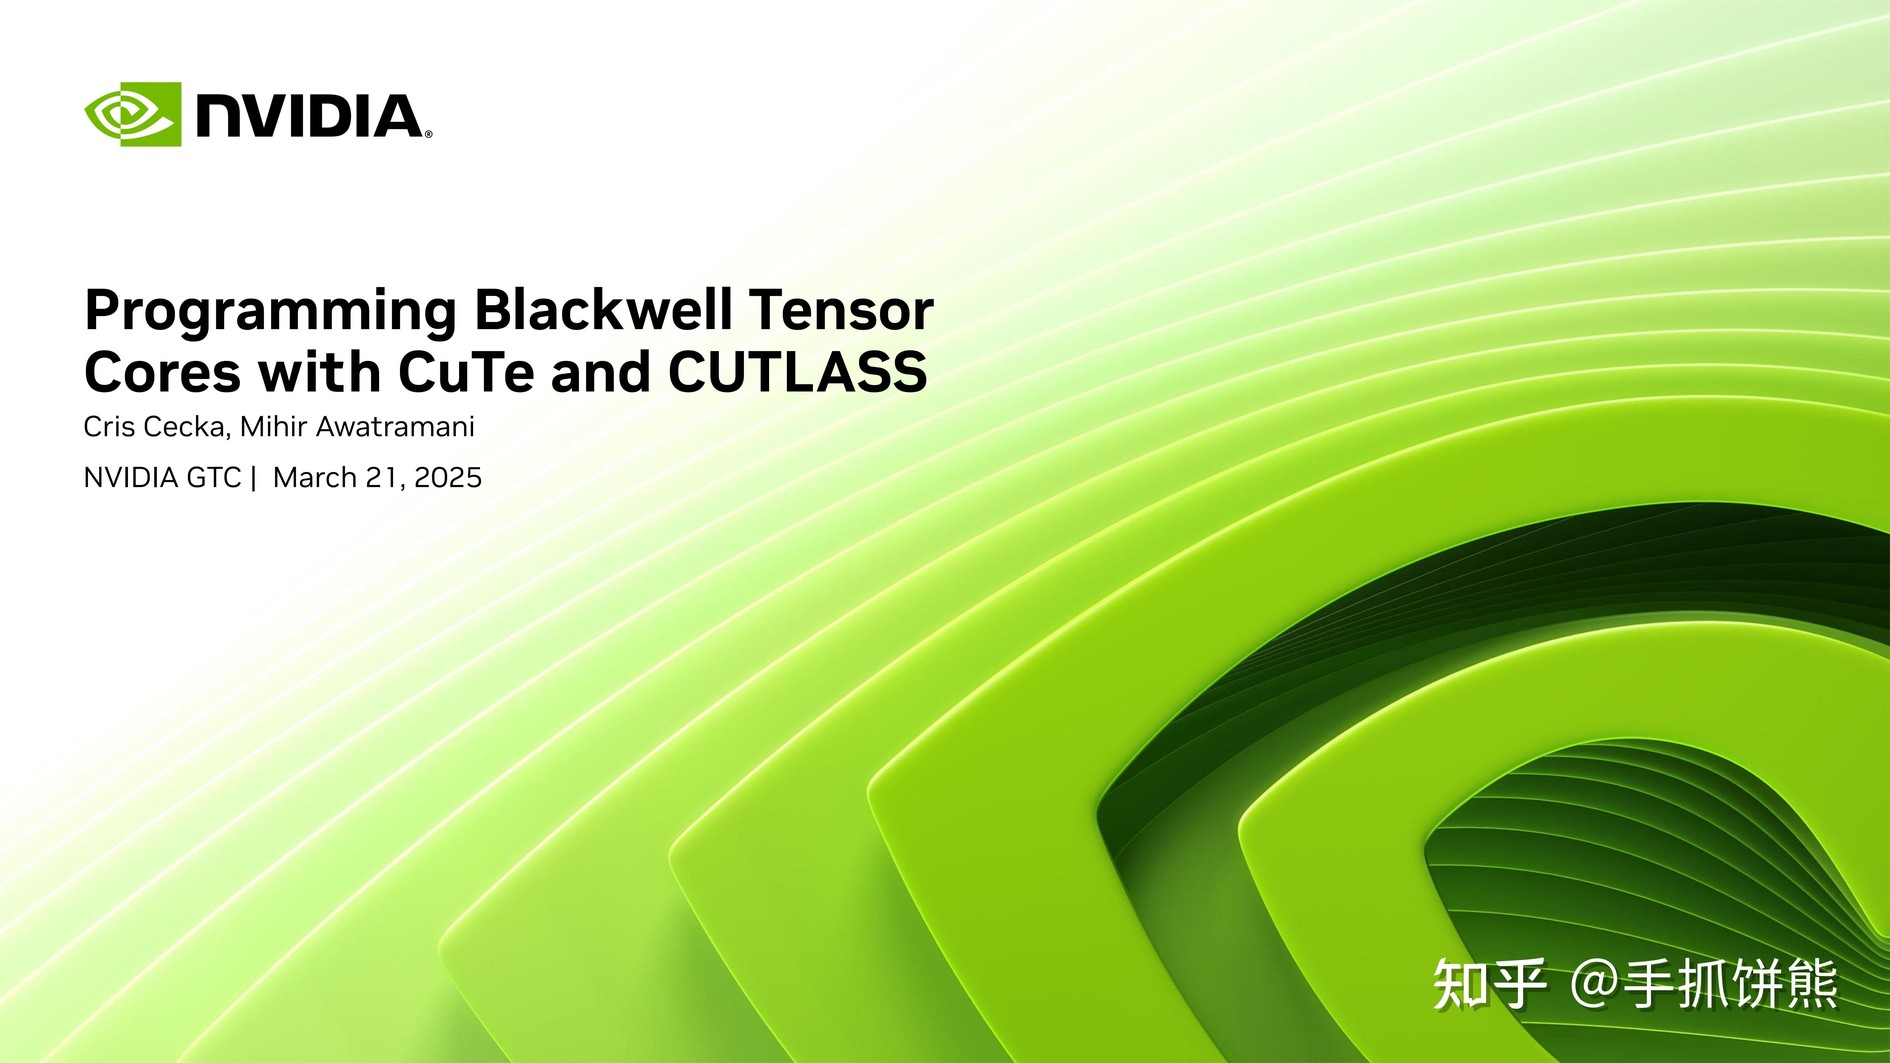
\includegraphics[width=0.9\textwidth]{figures/zhaoshangchun-01-tensor-core-programming/fig-01.jpg}
\end{figure}

这一页主要是封面部分，介绍作者和文章主题等。

\textbf{第 2 页：CUTLASS介绍}

\begin{figure}[H]\centering
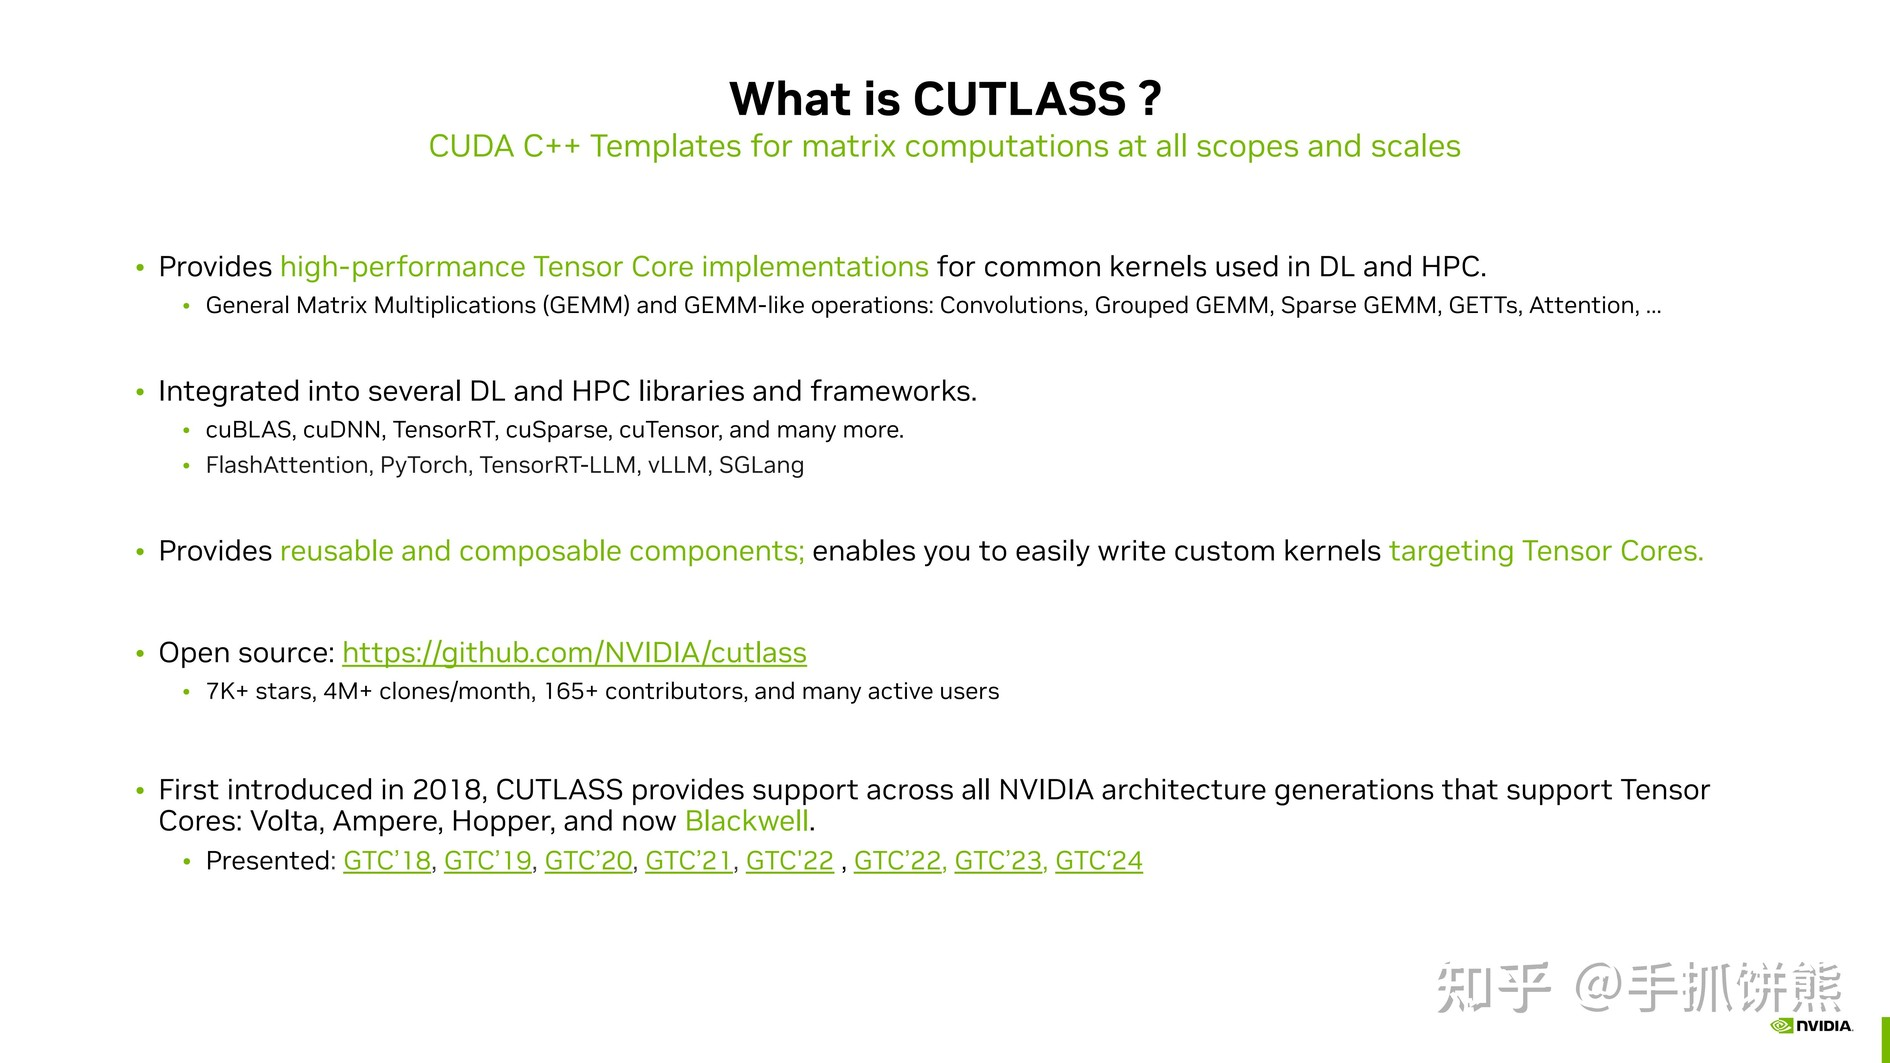
\includegraphics[width=0.9\textwidth]{figures/zhaoshangchun-01-tensor-core-programming/fig-02.jpg}
\end{figure}

CUTLASS \textbf{本质上是一个基于 C++ 模板的 CUDA 核函数库}，专门用于实现高性能的矩阵运算，特别是针对 Tensor Core 的优化。它提供了高度优化的 \texttt{GEMM} (通用矩阵乘法) 及其变种（如卷积、分组 GEMM、稀疏 GEMM 等）的实现。CUTLASS将这些复杂实现\textbf{分解为一系列可重用、可组合的模块化组件}。

CUTLASS 不仅是 NVIDIA 官方库（如 cu\allowbreak{}BLAS、cu\allowbreak{}DNN）的基石，也成为了 Py\allowbreak{}Torch、Tensor\allowbreak{}RT-LLM、Flash\allowbreak{}Attention 等业界顶级框架和项目的核心依赖。

对于算子优化工程师，CUTLASS 提供了一个强大的“乐高积木盒”，让你能基于这些高度抽象和封装的组件，快速构建针对特定场景的、接近硬件极限性能的自定义核函数，而无需从零开始手写复杂的 PTX (Parallel Thread Execution) 指令。

CUTLASS目前是开源的，且社区非常的活跃。

自 2018 年首次推出以来，CUTLASS 已经伴随 Volta、Ampere、Hopper 、Blackwell架构一路演进。

\textbf{第 3 页：本视频演讲的大纲}

\begin{figure}[H]\centering
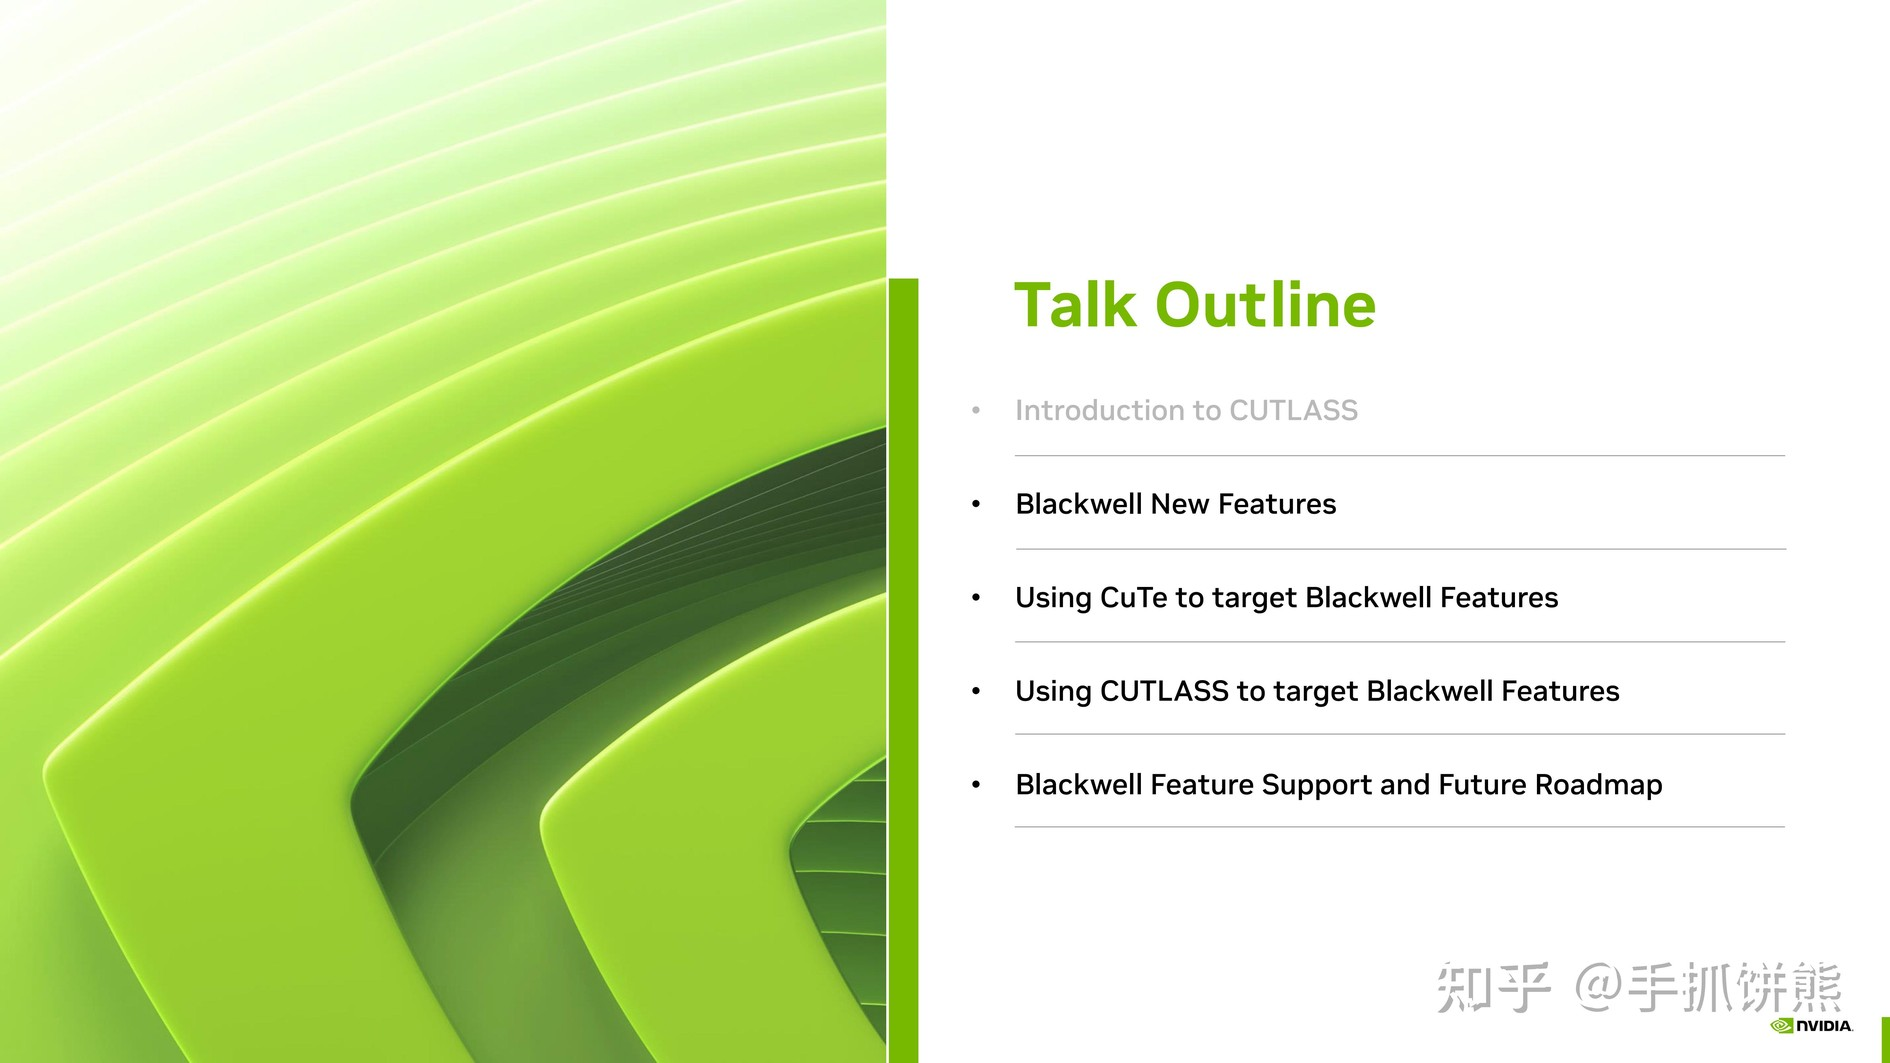
\includegraphics[width=0.9\textwidth]{figures/zhaoshangchun-01-tensor-core-programming/fig-03.jpg}
\end{figure}

这张幻灯片清晰地展示了本次演讲的大纲。

\begin{enumerate}
\item 首先简要回顾介绍一下 CUTLASS。
\item 然后介绍一下\textbf{Blackwell 架构的新特性}。
\item 从 \textbf{Cu\allowbreak{}Te} 层面，详细阐述如何利用这些新工具和库来使用Blackwell 的新功能。
\item 从 \textbf{CUTLASS} 层面，详细阐述如何利用这些新工具和库来使用Blackwell 的新功能。
\item 最后，以一个功能支持总结和未来路线图收尾。
\end{enumerate}

\section{\textbf{二、Blackwell 架构新特性}}

这一章是理解后续所有编程模型变化的基础，它系统性地介绍了 Blackwell 架构在硬件层面带来的三大核心革新：全新的\textbf{第五代 Tensor Core}、专为张量运算设计的 \textbf{Tensor Memory}(TMEM)，以及更灵活、\textbf{更高效的调度能力}。

\textbf{第 4 页：Blackwell 架构新特性概览}

\begin{figure}[H]\centering
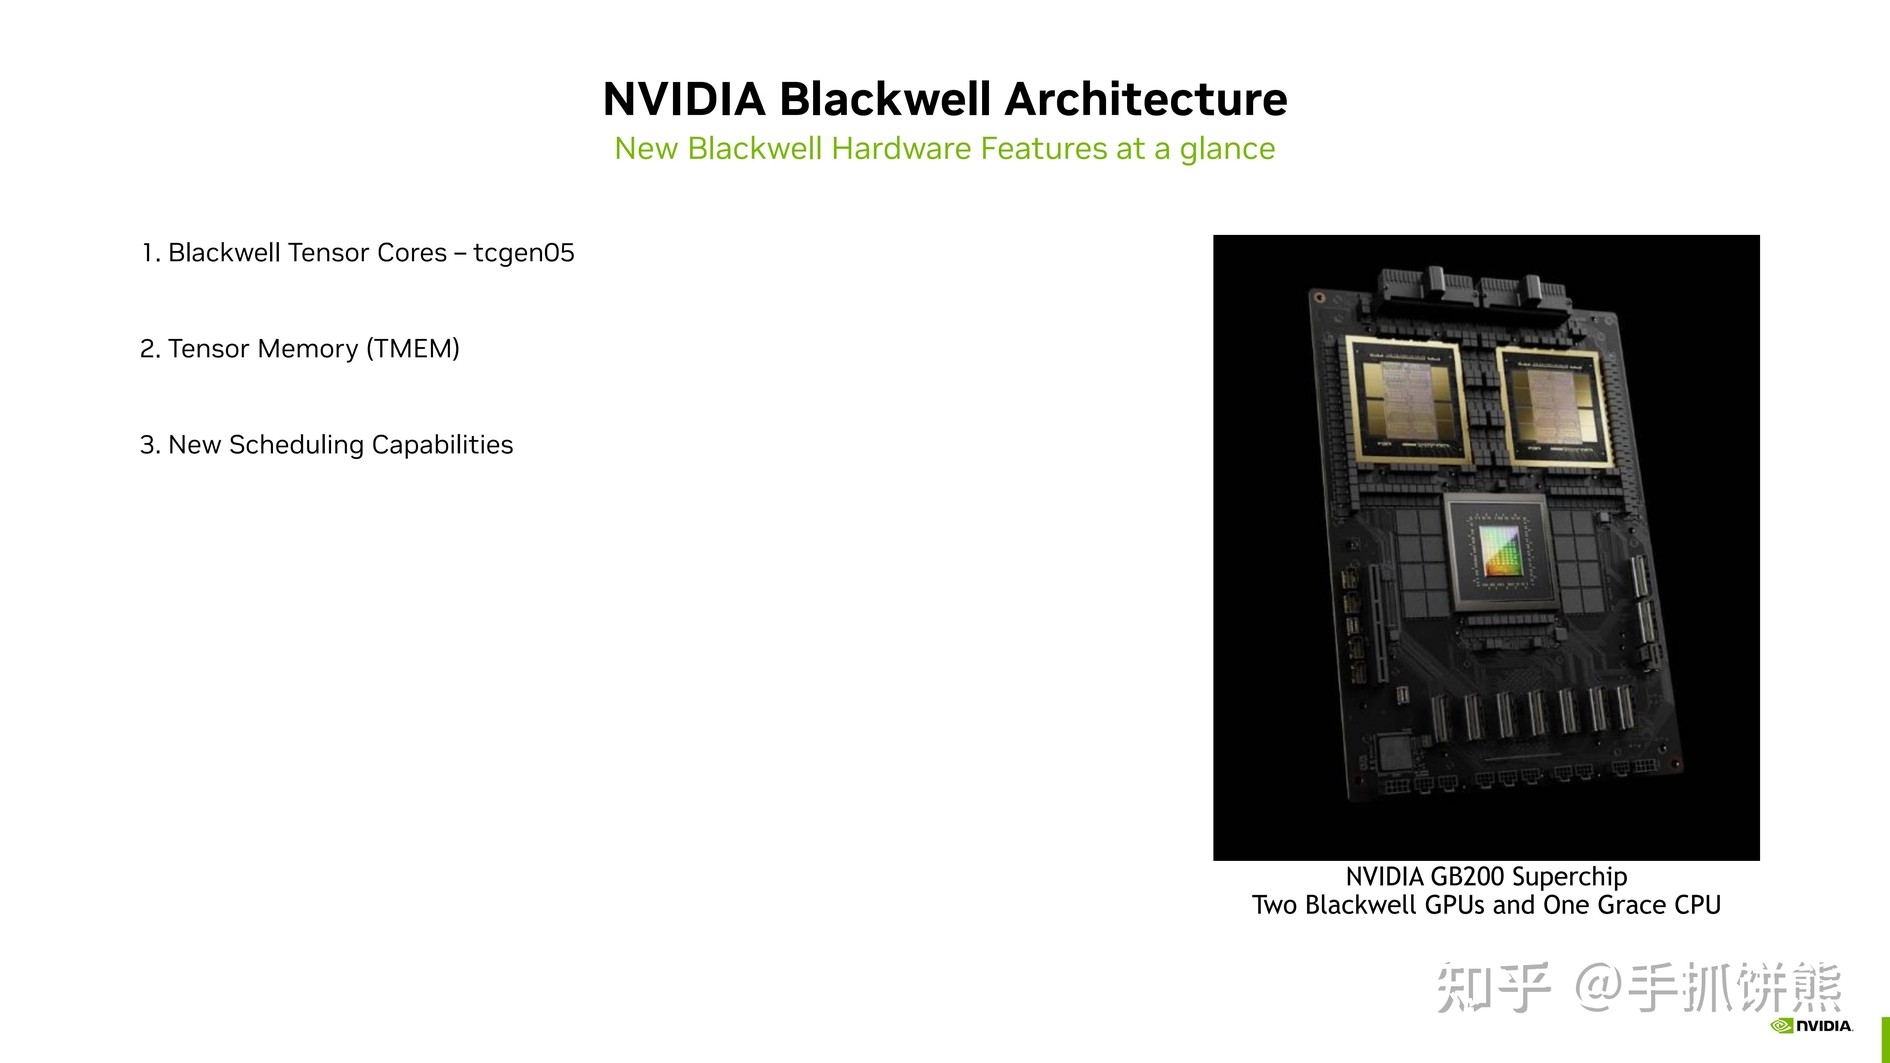
\includegraphics[width=0.9\textwidth]{figures/zhaoshangchun-01-tensor-core-programming/fig-04.jpg}
\end{figure}

这张幻灯片是对 Blackwell 架构三大核心硬件特性的高度概括。

\textbf{第一，第五代 Tensor Core (tcgen05)}，这是计算能力的核心引擎，带来了新的数据类型支持和更高的吞吐。

\textbf{第二，Tensor Memory (TMEM)}，一种新型的片上内存，专门用于服务于 Tensor Core 的输入和输出，旨在解决访存瓶颈。

\textbf{第三，新的调度能力 (New Scheduling Capabilities)}，包括对线程块簇（Thread Block Clusters）的优化和动态调度机制，旨在提升 GPU 的整体利用率和执行效率。

这三大特性共同构成了 Blackwell 性能飞跃的基石，后续的编程模型演进都将围绕它们展开。

右侧的 GB200 Superchip 图片展示了其宏伟的物理形态——两块 Blackwell GPU 与一块 Grace CPU 通过高达 900 GB/\allowbreak{}s 的 NVLink-C2\allowbreak{}C 高速互联紧密耦合。

\subsection{\textbf{第五代 Tensor Core}}

\textbf{第 5 页：从 Hopper 到 Blackwell 的 Tensor Core 演进}

\begin{figure}[H]\centering
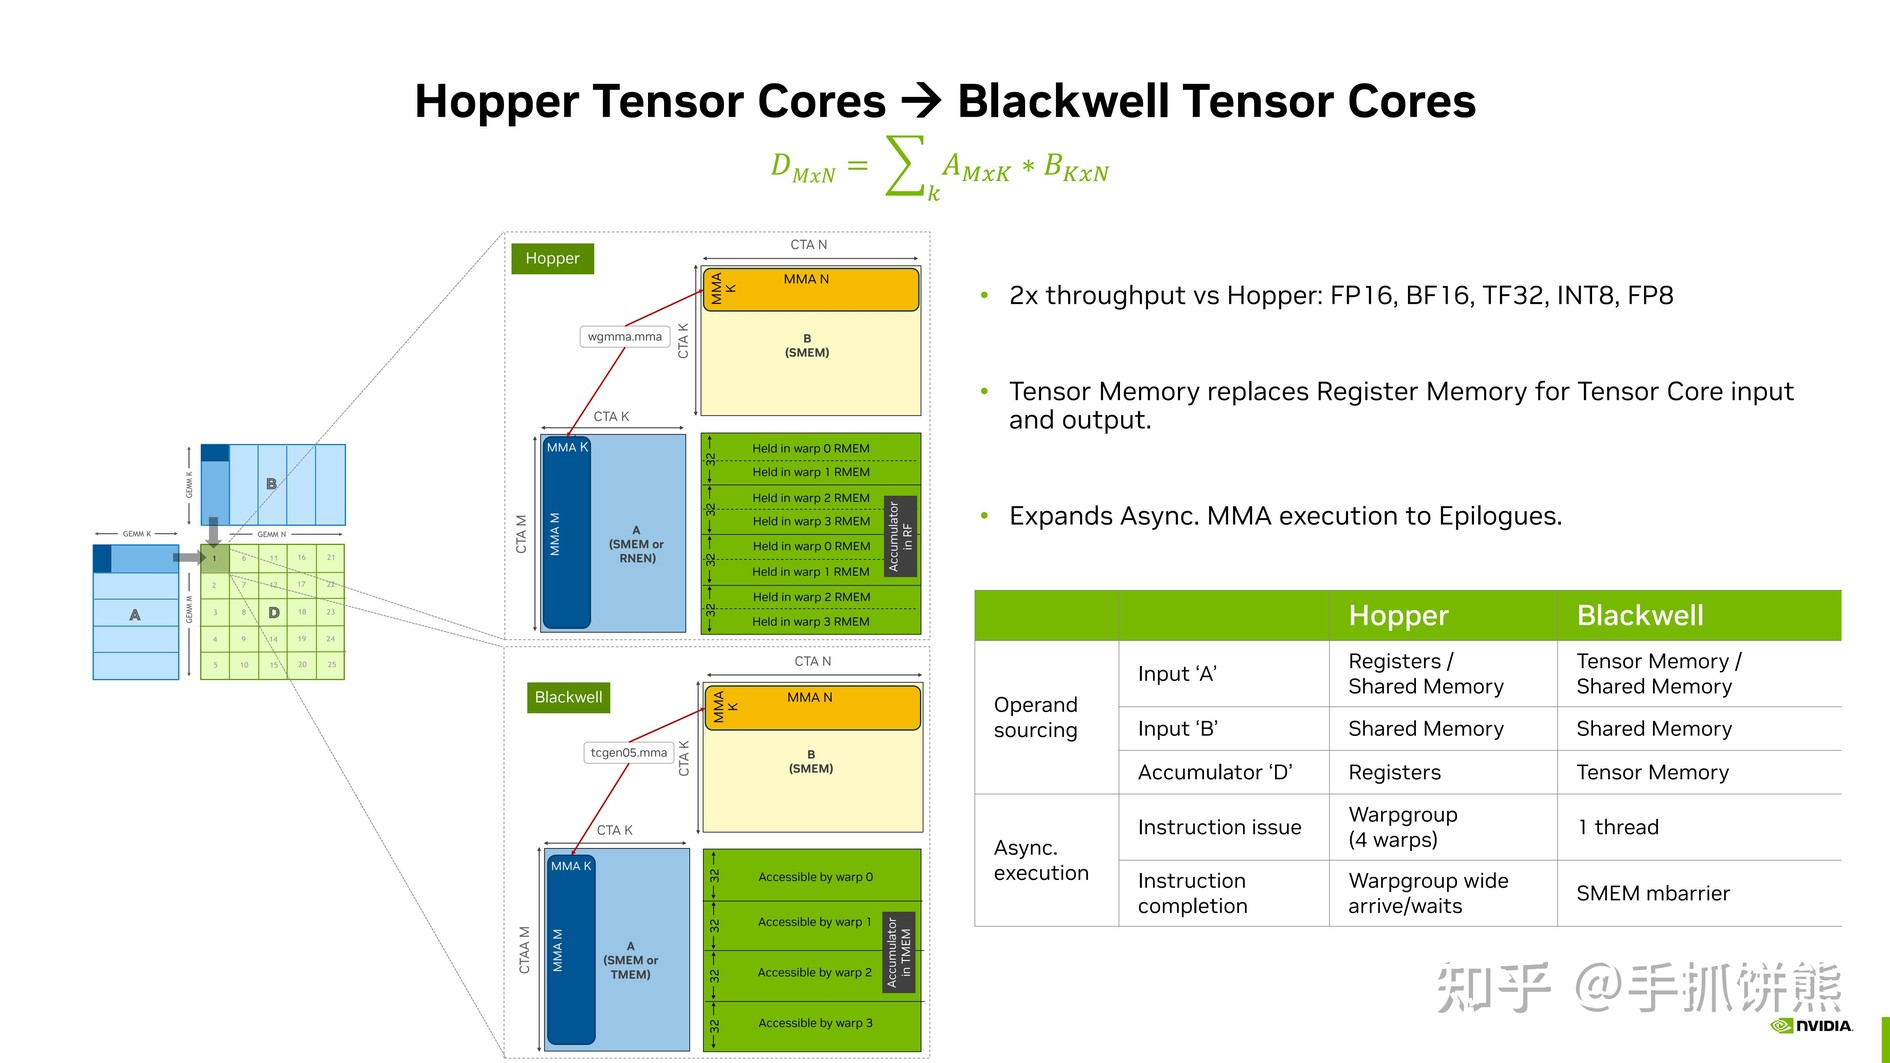
\includegraphics[width=0.9\textwidth]{figures/zhaoshangchun-01-tensor-core-programming/fig-05.jpg}
\end{figure}

这一页通过对比 Hopper 和 Blackwell 的 Tensor Core，揭示了 Blackwell \texttt{tcgen05} 的关键变化。最核心的变革在于\textbf{计算数据流的重塑}。

在 Hopper 上，MMA (Matrix Multiply-Accumulate) 指令的输入 A 矩阵可以来自寄存器（Register File）或共享内存（Shared Memory），累加结果 D 则存放在寄存器中。

而在 Blackwell 中，\textbf{输入 A 和累加结果 D 的主要存储位置都变成了新引入的 Tensor Memory (TMEM)}。这一改变意义深远，TMEM 作为一块专为张量操作设计的内存，能够更高效地暂存和流转数据，\textbf{减少对通用寄存器的压力}，为更大规模的异步计算铺平了道路。

表格中还指出了另一个关键点：\textbf{异步执行模型的扩展}。

Hopper 的异步 MMA 主要局限于计算阶段，\textbf{而 Blackwell 将其异步扩展到了 Epilogue}（收尾阶段，如结果写回、后处理等）。同时，指令的下发和同步机制也发生了变化。Hopper 的 \texttt{wgmma} (warpgroup mma) 由一个 warpgroup（4个 warp）共同执行，而 Blackwell 的 \texttt{tcgen05.\allowbreak{}mma} 则由单个线程下发，但其执行和同步可以跨越更广泛的范围（如整个 warpgroup 或 SM 级别的 mbarrier），这提供了更灵活的异步编程模型。

总而言之，Blackwell Tensor Core \textbf{通过引入 TMEM 和强化异步机制，实现了对 FP16/\allowbreak{}BF16/\allowbreak{}TF32/\allowbreak{}INT8/\allowbreak{}FP8 等数据类型翻倍的理论吞吐量}，这是其性能提升的核心来源。

\textbf{第 6 页：跨 SM 的 Tensor Core 执行}

\begin{figure}[H]\centering
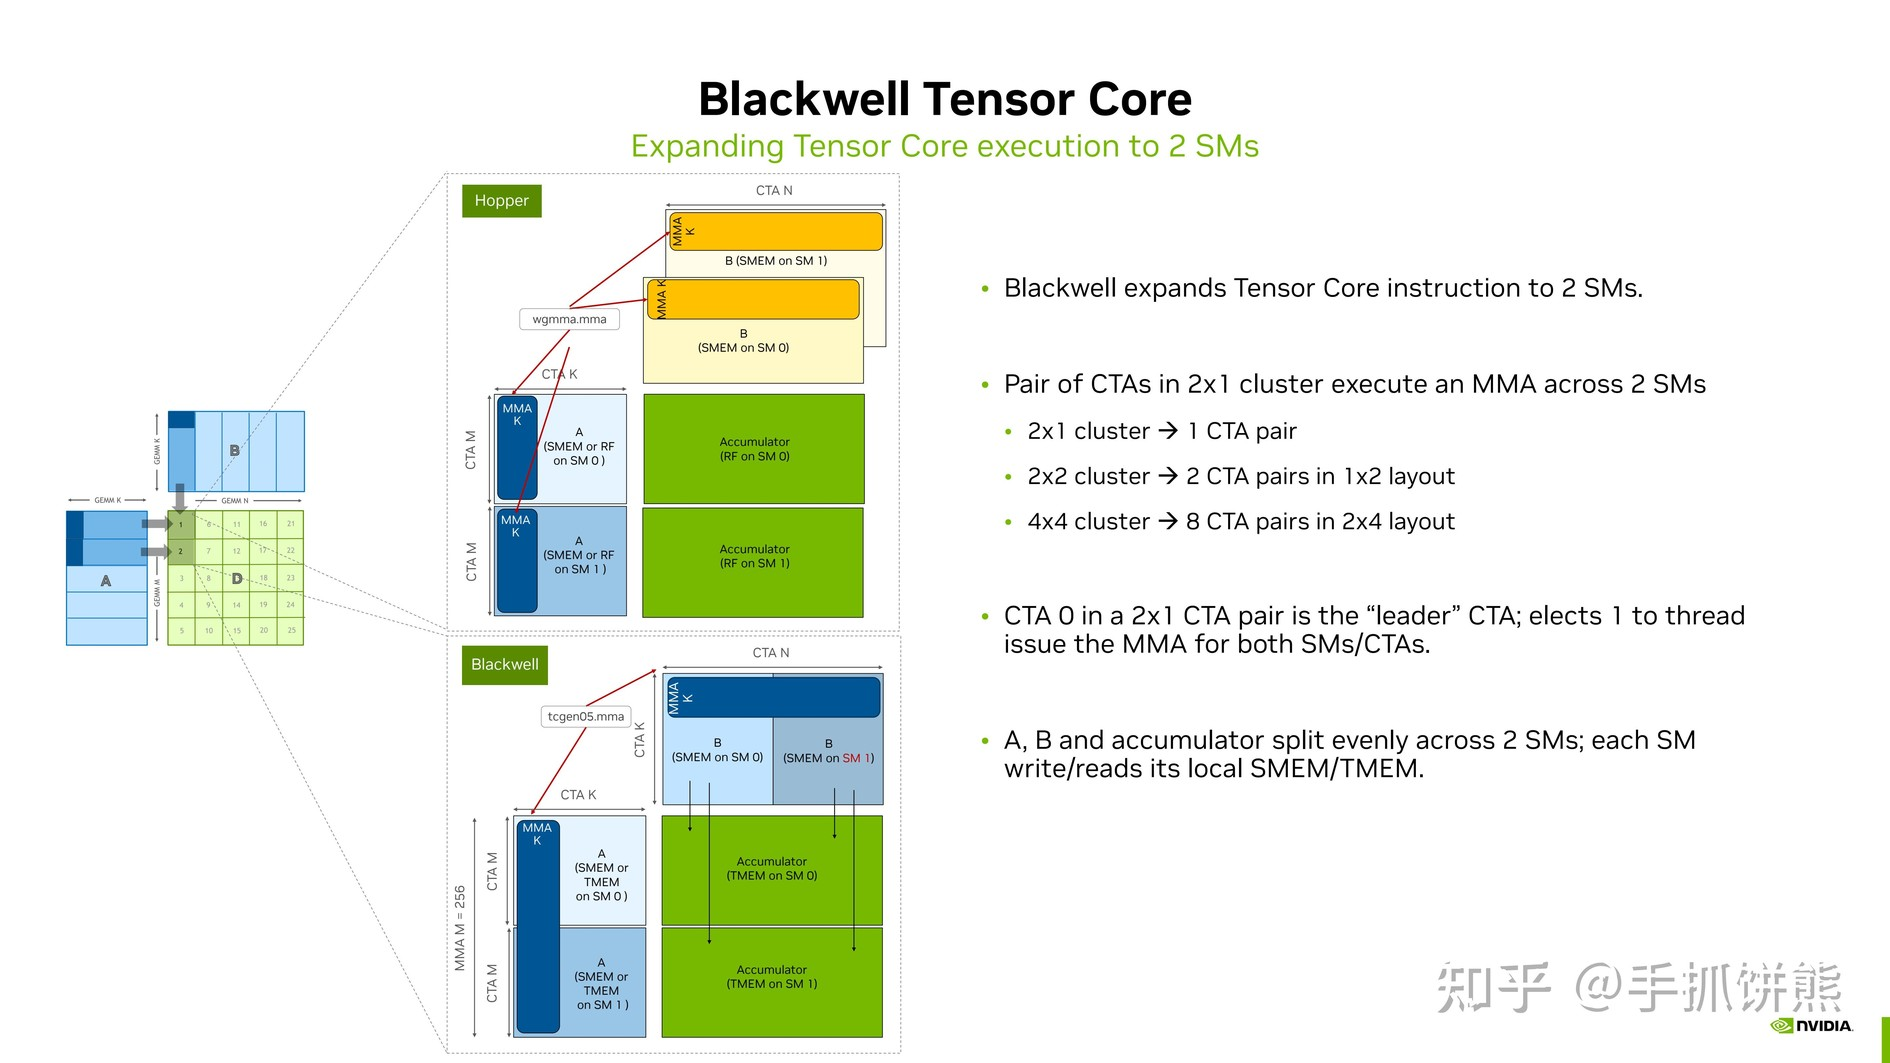
\includegraphics[width=0.9\textwidth]{figures/zhaoshangchun-01-tensor-core-programming/fig-06.jpg}
\end{figure}

这张图进一步揭示了 Blackwell 如何实现 Tensor Core 性能翻倍的秘密：\textbf{将 Tensor Core 指令的执行范围从单个 SM 扩展到了两个 SM}。在 Hopper 架构中，一个 CTA (Cooperative Thread Array) 内的 warpgroup 独立在其所在的 SM 上完成 MMA 计算。而在 Blackwell 中，引入了\textbf{跨 SM 的 MMA 执行机制}。一对位于 2x1 物理集群（Cluster）中的 CTAs 可以协同执行一个 MMA 指令。其中一个 CTA（leader CTA）里的某个线程负责下发指令，但计算任务（包括 A、B 矩阵的读取和累加器的计算）则\textbf{平均分配到两个 SM 上并行处理}。

这意味着单个 MMA 指令能够调用的计算资源和片上内存（SMEM/\allowbreak{}TMEM）都直接翻倍，\textbf{从而支撑起更大的 MMA M 维度（例如从 Hopper 的 128 扩展到 Blackwell 的 256），这是实现 2 倍吞吐量的直接原因}。这种 \textbf{2-SM-MMA} 的设计，要求编程模型必须能够感知和管理跨 SM 的数据和同步，这也是 Cu\allowbreak{}Te 和 CUTLASS 4.0 中引入\texttt{2\allowbreak{}SM}相关抽象的根本原因。开发者需要适应这种新的 CTA-Pair 协作模式，以编写出能够充分利用 Blackwell 硬件能力的核函数。

\textbf{第 7 页：新增的block-scale数据类型支持}

\begin{figure}[H]\centering
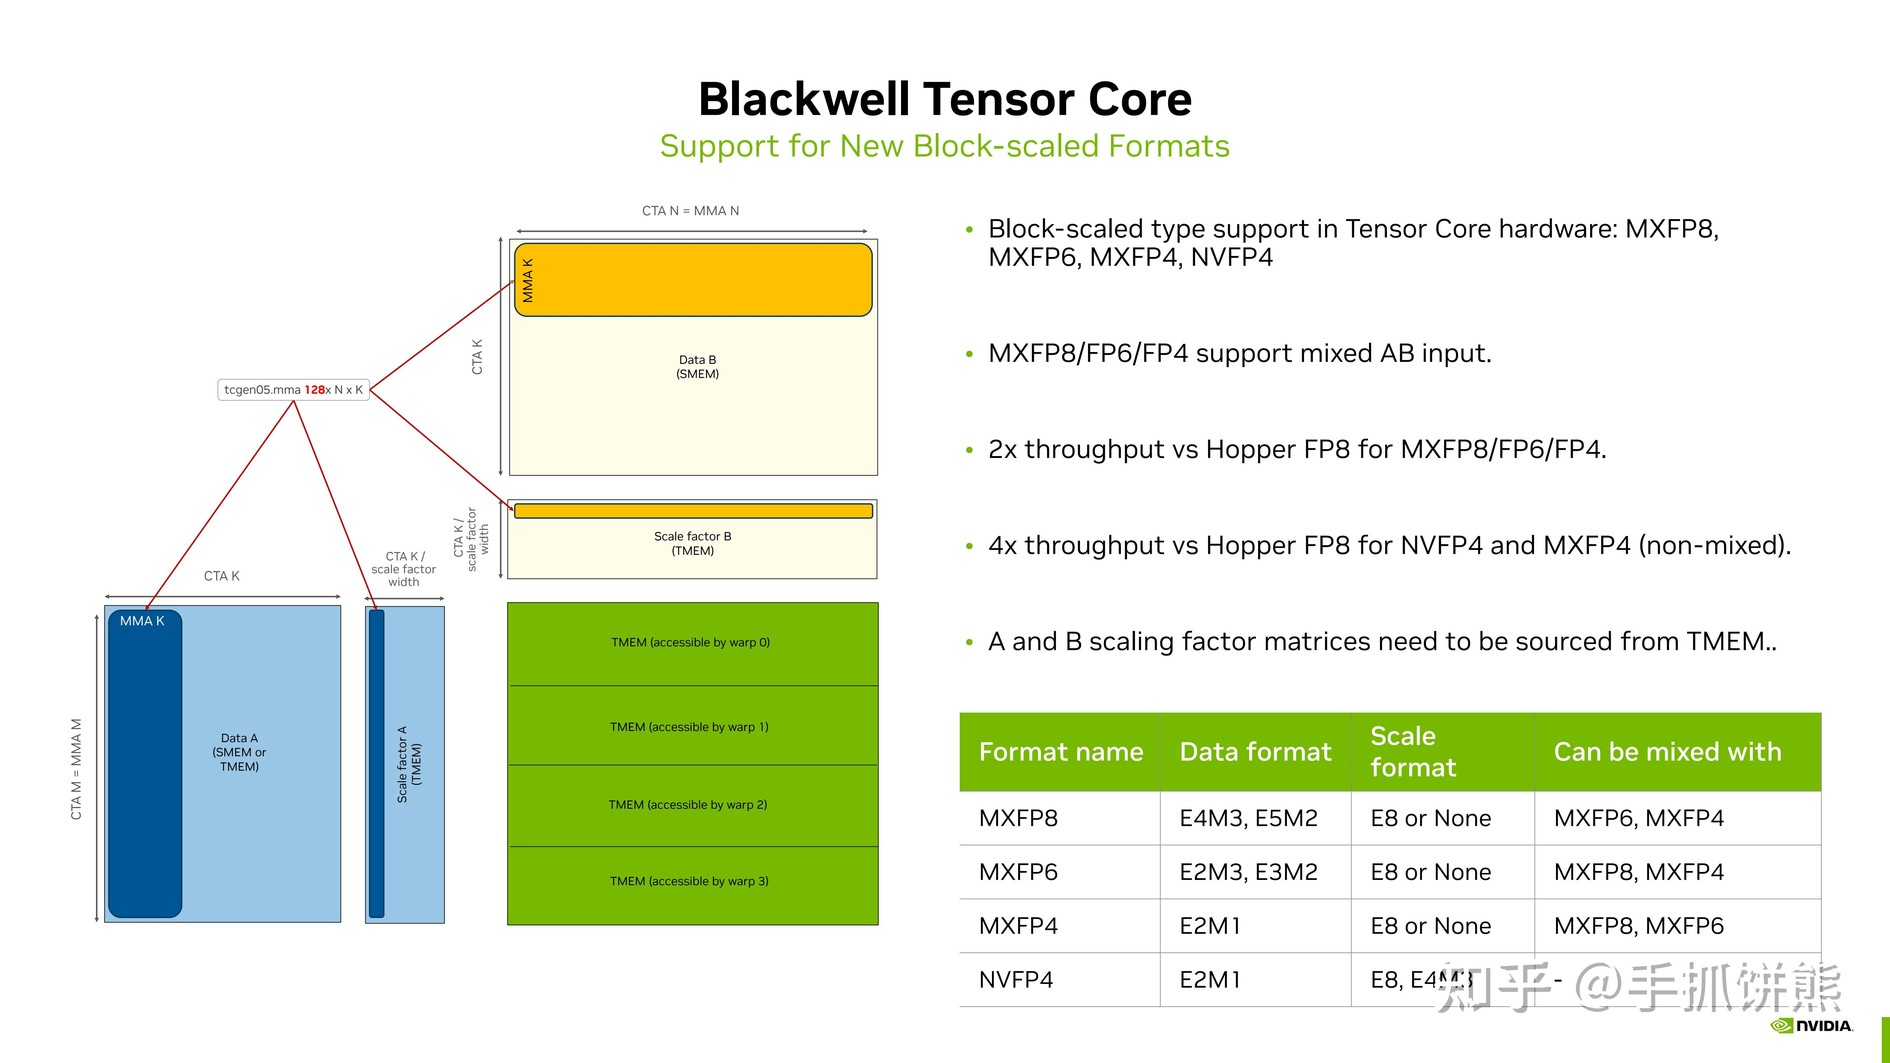
\includegraphics[width=0.9\textwidth]{figures/zhaoshangchun-01-tensor-core-programming/fig-07.jpg}
\end{figure}

Blackwell Tensor Core 的另一大亮点是\textbf{硬件原生支持了新的block-scale量化方式}，包括 MXFP8、MXFP6、MXFP4、以及 NVIDIA 的 NVFP4。这些低比特格式对于追求极致性能和压缩率的推理场景至关重要。所谓block-scale，是指一个数据块（tile）共享一个或多个缩放因子（scaling factor），从而可以用更少的比特表示更大范围的数值，这是在精度和性能之间取得平衡的关键技术。

从图中可以看到，\texttt{tcgen05.\allowbreak{}mma} 指令在计算时，除了加载数据 A 和 B，还需要从 TMEM 中加载它们各自的\textbf{缩放因子矩阵 (Scale factor A/\allowbreak{}B)}。硬件会自动处理反量化和计算过程。更具吸引力的是，Blackwell 支持\textbf{混合输入 (mixed AB input)}，例如 A 矩阵使用 MXFP8，B 矩阵使用 MXFP4，这为非对称量化等高级优化策略提供了硬件层面的支持。性能上，MXFP8/\allowbreak{}FP6/\allowbreak{}FP4 相比 Hopper FP8 实现了 \textbf{2 倍吞吐量}，而 NVFP4 和非混合的 MXFP4 更是达到了惊人的 \textbf{4 倍吞吐量}。这意味着在可接受的精度损失下，推理性能可以获得巨大提升，直接降低大模型服务的成本。

\textbf{第 8 页：Blackwell 架构新特性概览}

\begin{figure}[H]\centering
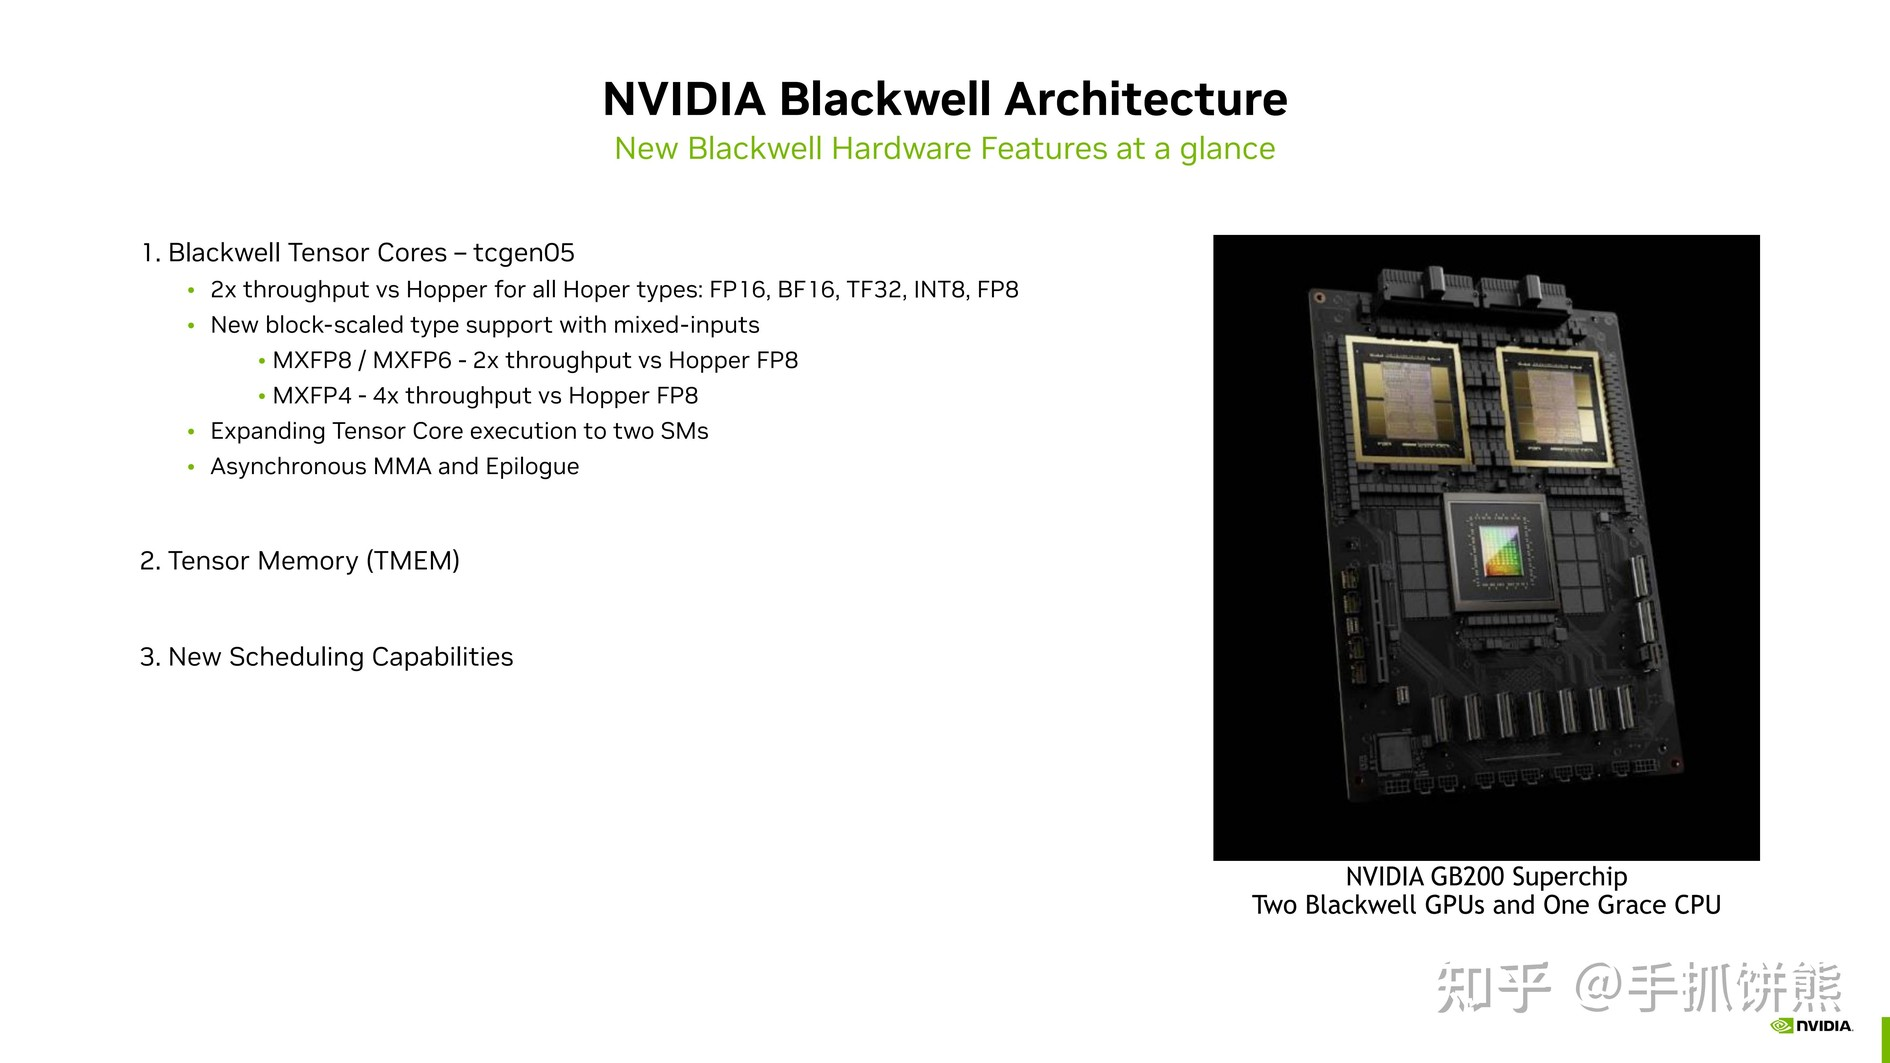
\includegraphics[width=0.9\textwidth]{figures/zhaoshangchun-01-tensor-core-programming/fig-08.jpg}
\end{figure}

这一页是对第一部分“Blackwell Tensor Cores”新特性的总结。它重申了几个关键点：

\begin{enumerate}
\item \textbf{吞吐量翻倍}：对于 Hopper 支持的所有数据类型（FP16、BF16、TF32、INT8、FP8），Blackwell 实现了 2 倍的理论性能。
\item \textbf{新的低比特格式}：引入了 MXFP8/\allowbreak{}MXFP6/\allowbreak{}MXFP4 等块缩放格式，最高可达 Hopper FP8 性能的 4 倍。
\item \textbf{跨 SM 执行}：Tensor Core 计算可以跨越两个 SM，这是性能翻倍的关键物理基础。
\item \textbf{全异步编程模型}：异步能力从计算扩展到了 Epilogue。
\end{enumerate}

\subsection{\textbf{Tensor Memory (TMEM)}}

\textbf{第 9 页：Tensor Memory (TMEM) 详解}

\begin{figure}[H]\centering
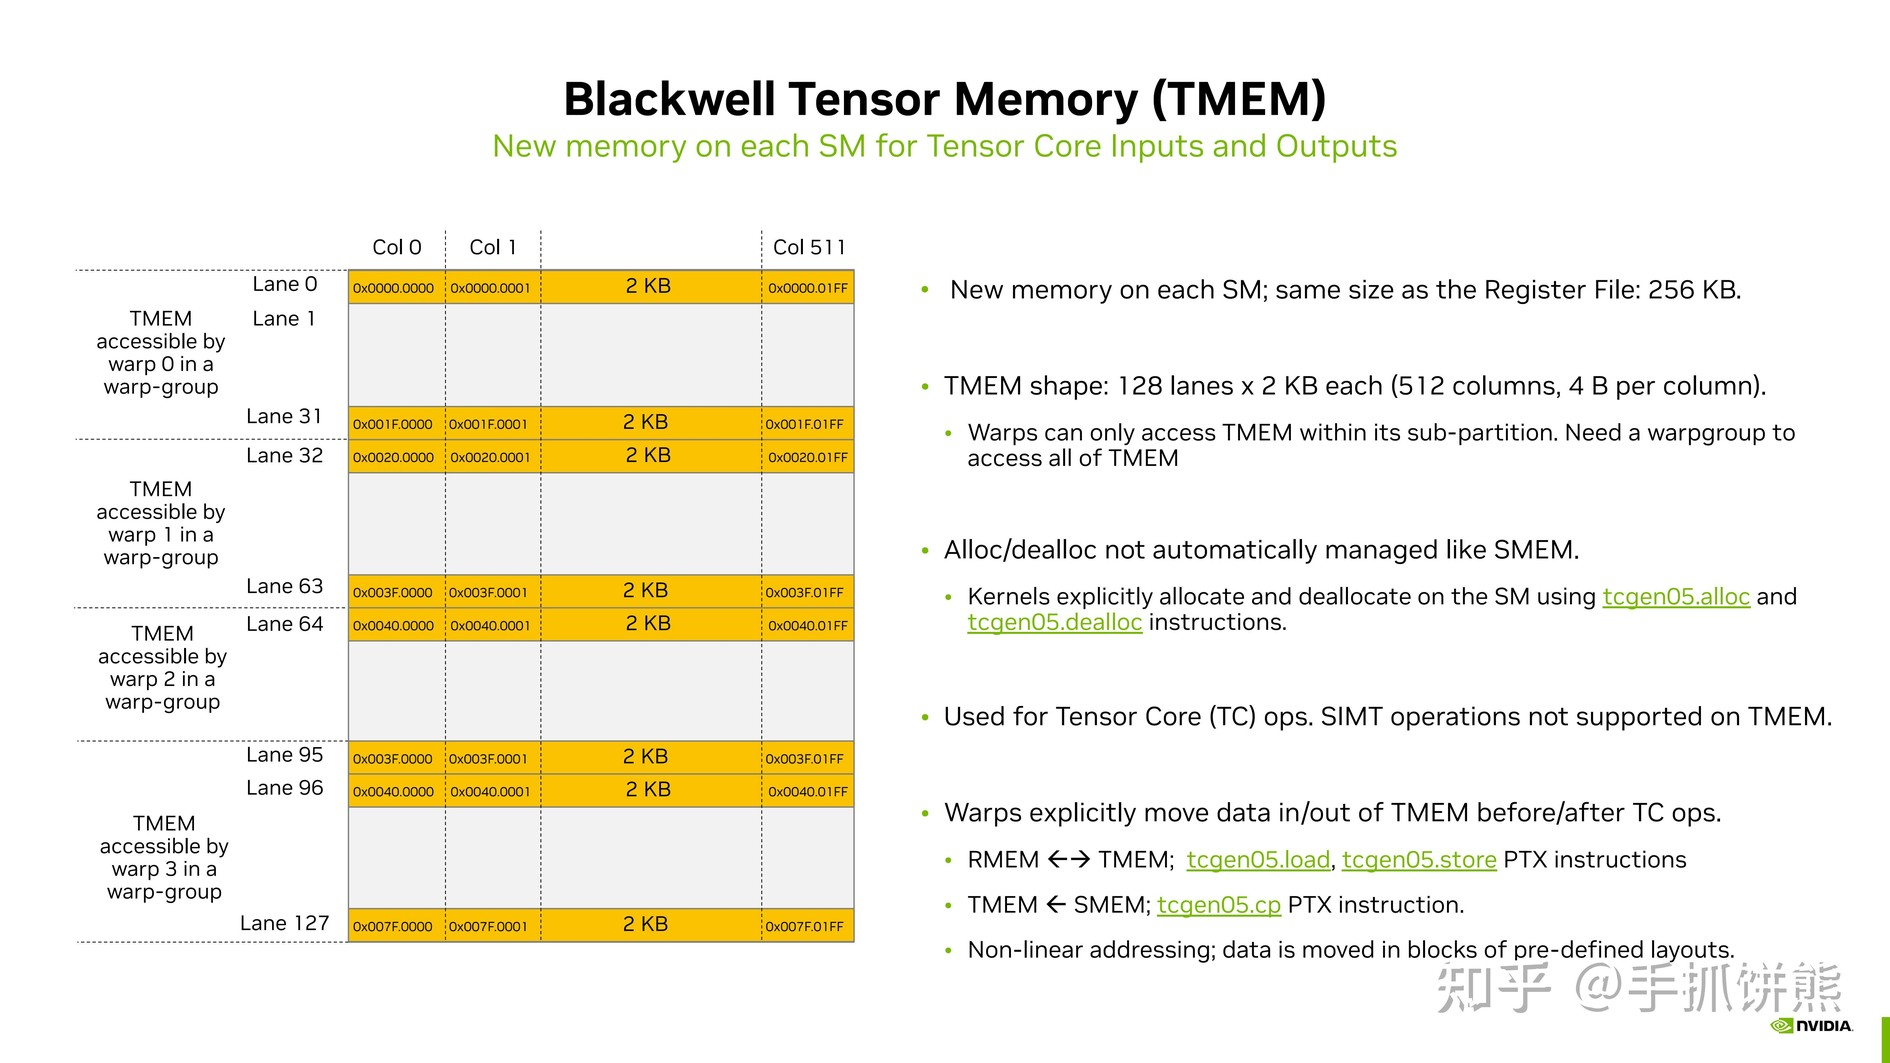
\includegraphics[width=0.9\textwidth]{figures/zhaoshangchun-01-tensor-core-programming/fig-09.jpg}
\end{figure}

这一页详细解读了 \textbf{Tensor Memory (TMEM)} 的物理结构和访问特性。

如左图所示，TMEM 是 Blackwell 每个 SM 上新增的一块 \textbf{256\allowbreak{}KB} 的片上内存，其容量与寄存器文件（Register File）相同。

它的物理结构被组织为 \textbf{128 个 lane，每个 lane 2\allowbreak{}KB}，总共 512 列（每列 4\allowbreak{}B）。一个关键的访问限制是：\textbf{一个 warpgroup（由 4 个 warp 组成）内的每个 warp 只能访问其对应的 32 个 lane}。这意味着单个 warp 无法访问整个 TMEM，必须由整个 warpgroup 协同才能完全利用。

与 SMEM (Shared Memory) 的自动管理不同，TMEM 的生命周期需要\textbf{由内核显式管理}。开发者需要使用新的 PTX 指令 \texttt{tcgen05.\allowbreak{}alloc} 和 \texttt{tcgen05.\allowbreak{}dealloc} 来手动分配和释放 TMEM 空间。

\textbf{TMEM 仅供 Tensor Core 操作使用，不支持通用的 SIMT (Single Instruction, Multiple Threads) 指令}。

数据必须通过特定的 PTX 指令在 TMEM 与寄存器（\texttt{tcgen05.\allowbreak{}load/\allowbreak{}store}）或 SMEM（\texttt{tcgen05.\allowbreak{}cp}）之间进行搬运，并且这些搬运操作基于预定义的块布局（block of pre-defined layouts），而非线性的字节地址。这增加了编程复杂度，但其目的是将张量数据从通用内存中解耦，形成专用高速通道，最大化 Tensor Core 利用率。

\textbf{第 10 页：Blackwell 架构新特性概览（再次更新）}

\begin{figure}[H]\centering
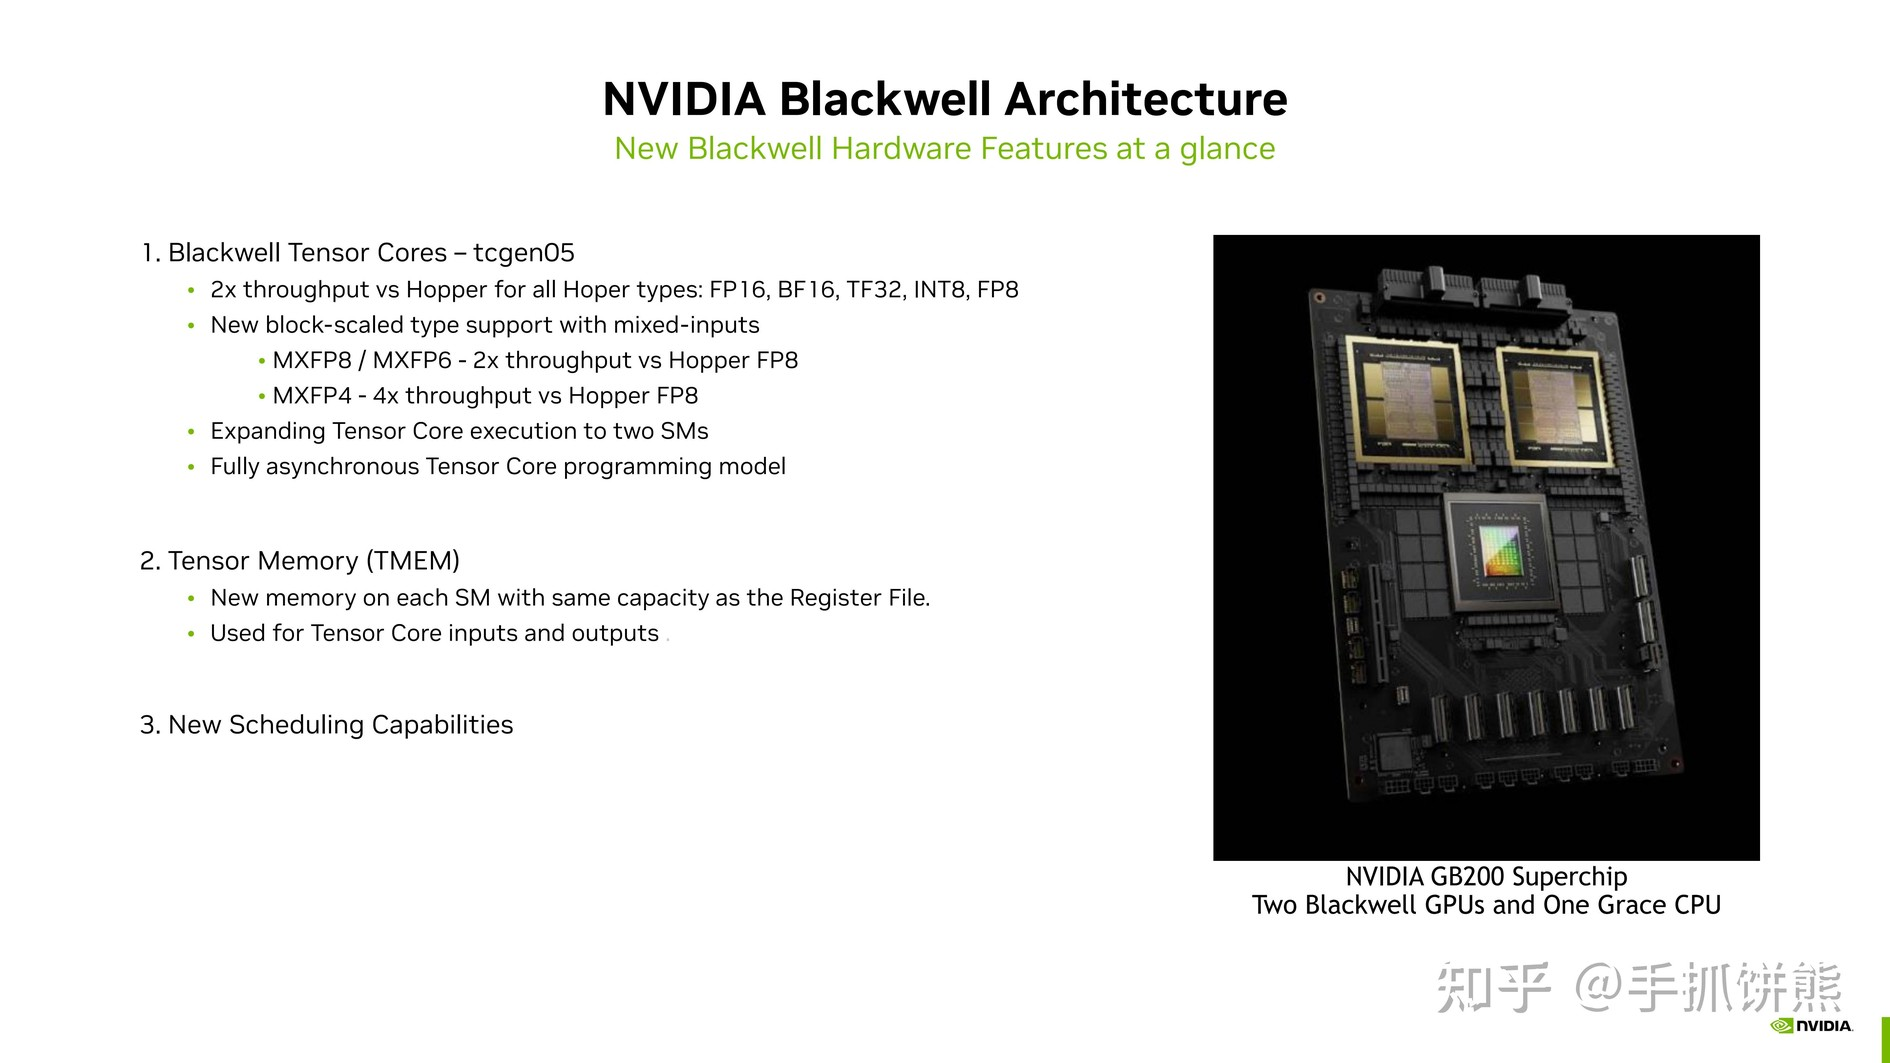
\includegraphics[width=0.9\textwidth]{figures/zhaoshangchun-01-tensor-core-programming/fig-10.jpg}
\end{figure}

这页在之前的总结上，加入了对 TMEM 的描述。此时，应该对 Blackwell 的两大硬件革新——\textbf{第五代 Tensor Core 和 TMEM 有了清晰的认识}。这一页再次强调，TMEM 是一块与寄存器文件容量相同的新增片上内存，其核心用途是\textbf{作为 Tensor Core 的输入和输出暂存区}。

\subsection{新的调度能力}

\textbf{第 11 页：首选线程块簇（Preferred Thread Block Clusters）}

\begin{figure}[H]\centering
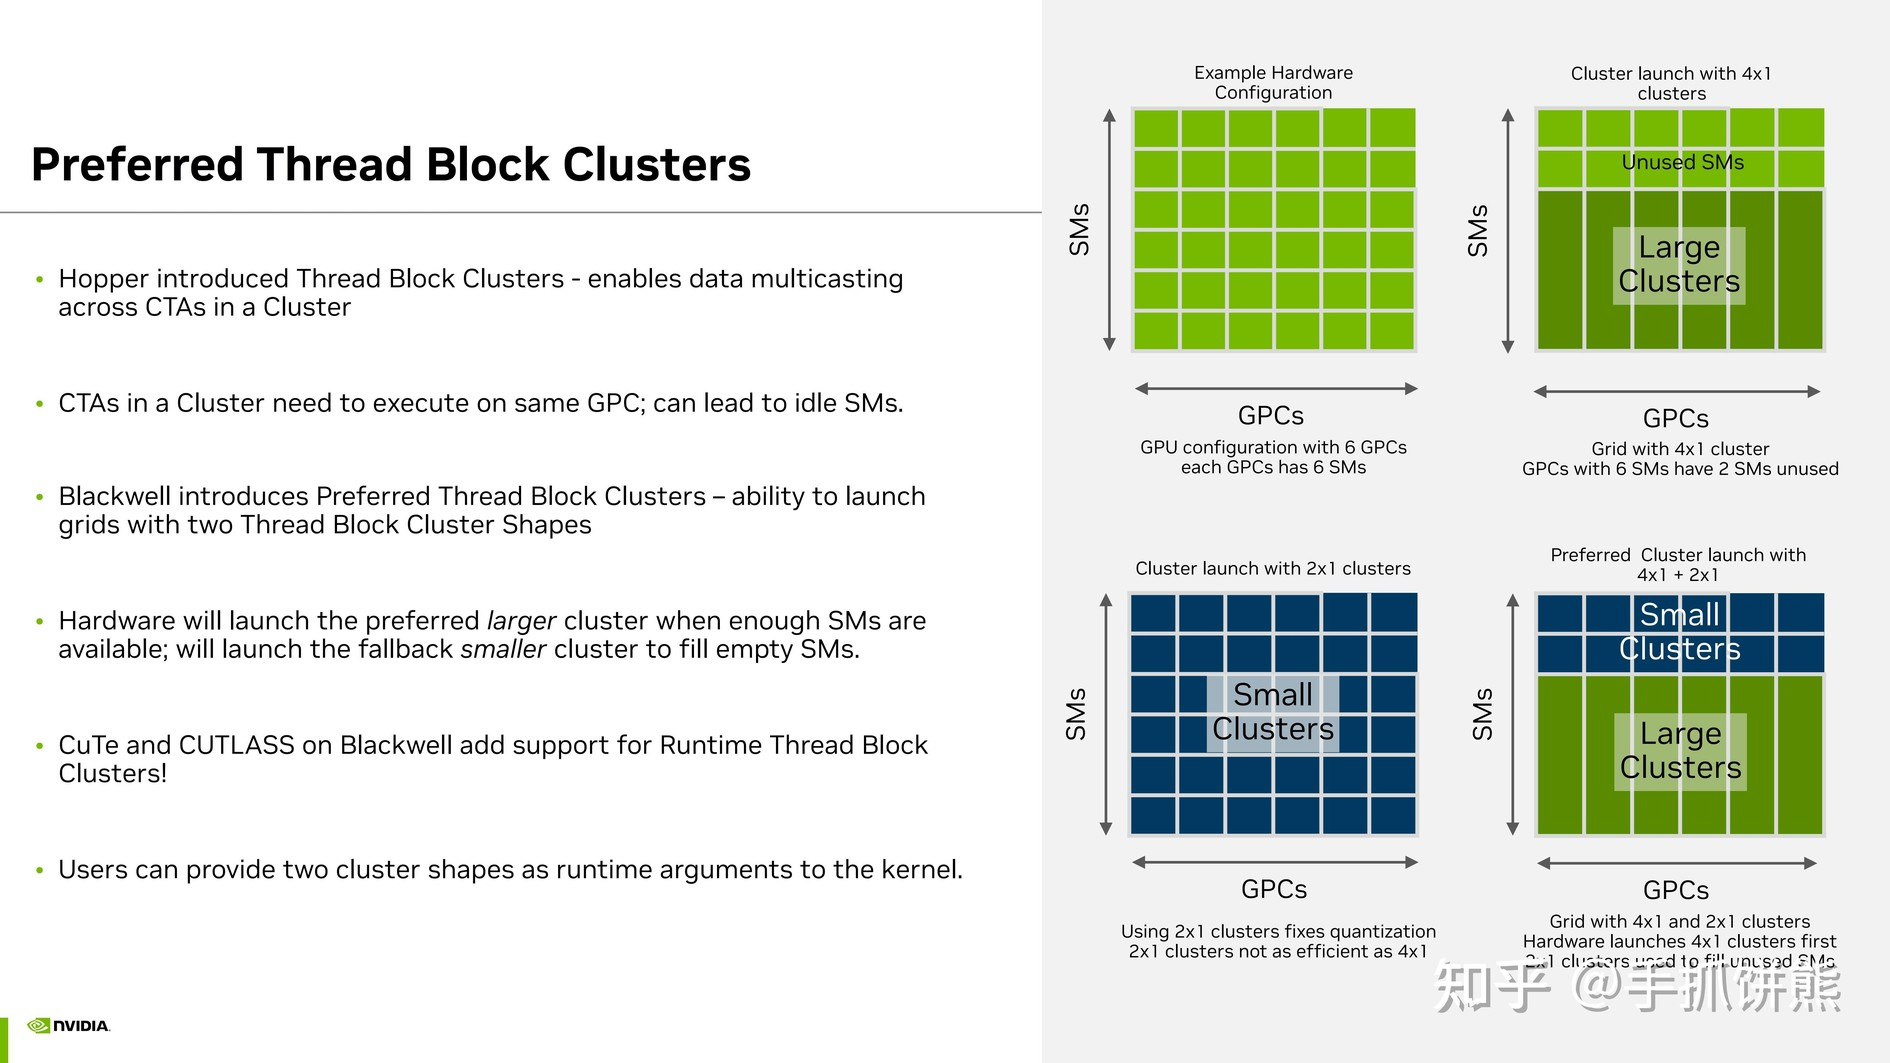
\includegraphics[width=0.9\textwidth]{figures/zhaoshangchun-01-tensor-core-programming/fig-11.jpg}
\end{figure}

这一页介绍了 Blackwell 在调度层面的第一个重要改进：\textbf{首选线程块簇 (Preferred Thread Block Clusters)}。

Hopper 架构引入了线程块簇（Cluster）的概念，允许一个 Cluster 内的多个 CTAs 协同工作并共享数据。但 Hopper 的静态 Cluster 调度存在一个问题：如果一个 Grid 被划分为固定大小的 Cluster（例如 4x1），而硬件的 GPC (Graphics Processing Cluster) 拥有的 SM 数量不是 Cluster 大小的整数倍（如图中每个 GPC 有 6 个 SM），就会导致 \textbf{SM 碎片化和闲置}。如图所示，启动 4x1 的 Cluster 会让每个 GPC 浪费 2 个 SM。

Blackwell 对此提出的解决方案是\textbf{允许一个 Grid 同时使用两种 Cluster Shape}：一个“首选”的较大尺寸（如 4x1）和一个“备用”的较小尺寸（如 2x1）。硬件调度器会\textbf{优先使用大尺寸的 Cluster 来填充大部分 SM，然后用小尺寸的 Cluster 去“填缝”}，从而最大限度地利用所有可用的 SM 资源。更妙的是，CUTLASS on Blackwell 支持\textbf{运行时指定 Cluster Shapes}，让开发者可以根据具体的 GPU 型号和问题规模，在内核启动时动态传入最佳的 Cluster 组合，进一步提升了性能的可移植性和优化灵活性。

\textbf{第 12 页：静态分块调度的问题}

\begin{figure}[H]\centering
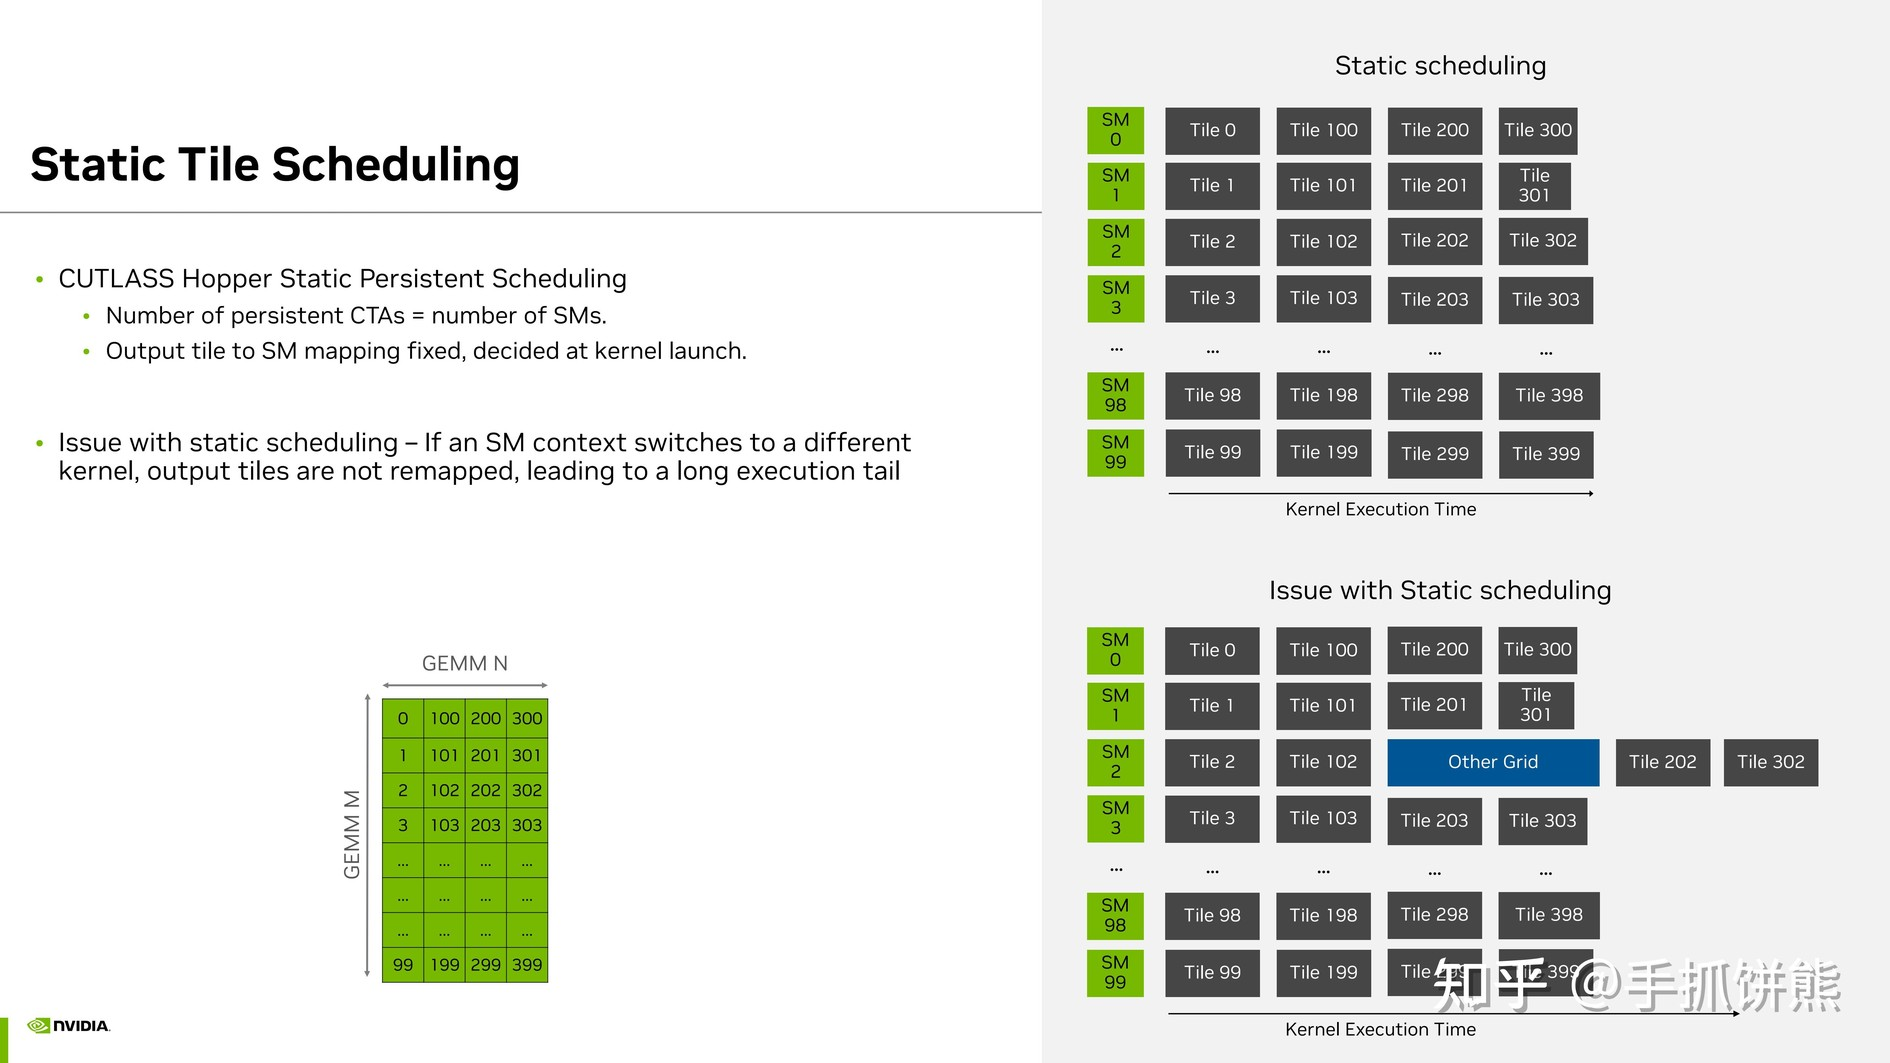
\includegraphics[width=0.9\textwidth]{figures/zhaoshangchun-01-tensor-core-programming/fig-12.jpg}
\end{figure}

此页直观地展示了 Hopper 上\textbf{静态持久调度 (Static Persistent Scheduling)} 的一个潜在缺陷。在持久化内核（persistent kernel，常用于 GEMM 等计算密集型任务）中，为了减少启动开销，通常会启动与 \textbf{SM 数量相等的持久化 CTA}。每个 CTA 负责处理输出矩阵的一部分 tiles（分块）。在静态调度模式下，\textbf{输出 tile 到 SM 的映射关系在内核启动时就固定了}。例如，SM 0 负责处理 tile 0, 100, 200...，SM 1 负责处理 tile 1, 101, 201...。

这种静态映射在理想情况下工作良好。但如果某个 SM（如图中的 SM 1）在执行过程中被操作系统或其他 CUDA grid \textbf{抢占}（context switch），它就需要先完成其他任务才能回来继续处理自己的 tile。由于其他 SM 并不会“帮助”被抢占的 SM，这会导致\textbf{严重的负载不均和长尾效应}。如图右侧所示，当其他 SM 都已完成工作进入空闲时，SM 1 还在“补作业”，整个 Grid 的执行时间被这根“长尾”严重拖慢，导致 GPU 整体利用率下降。

\textbf{第 13 页：动态分块调度}

\begin{figure}[H]\centering
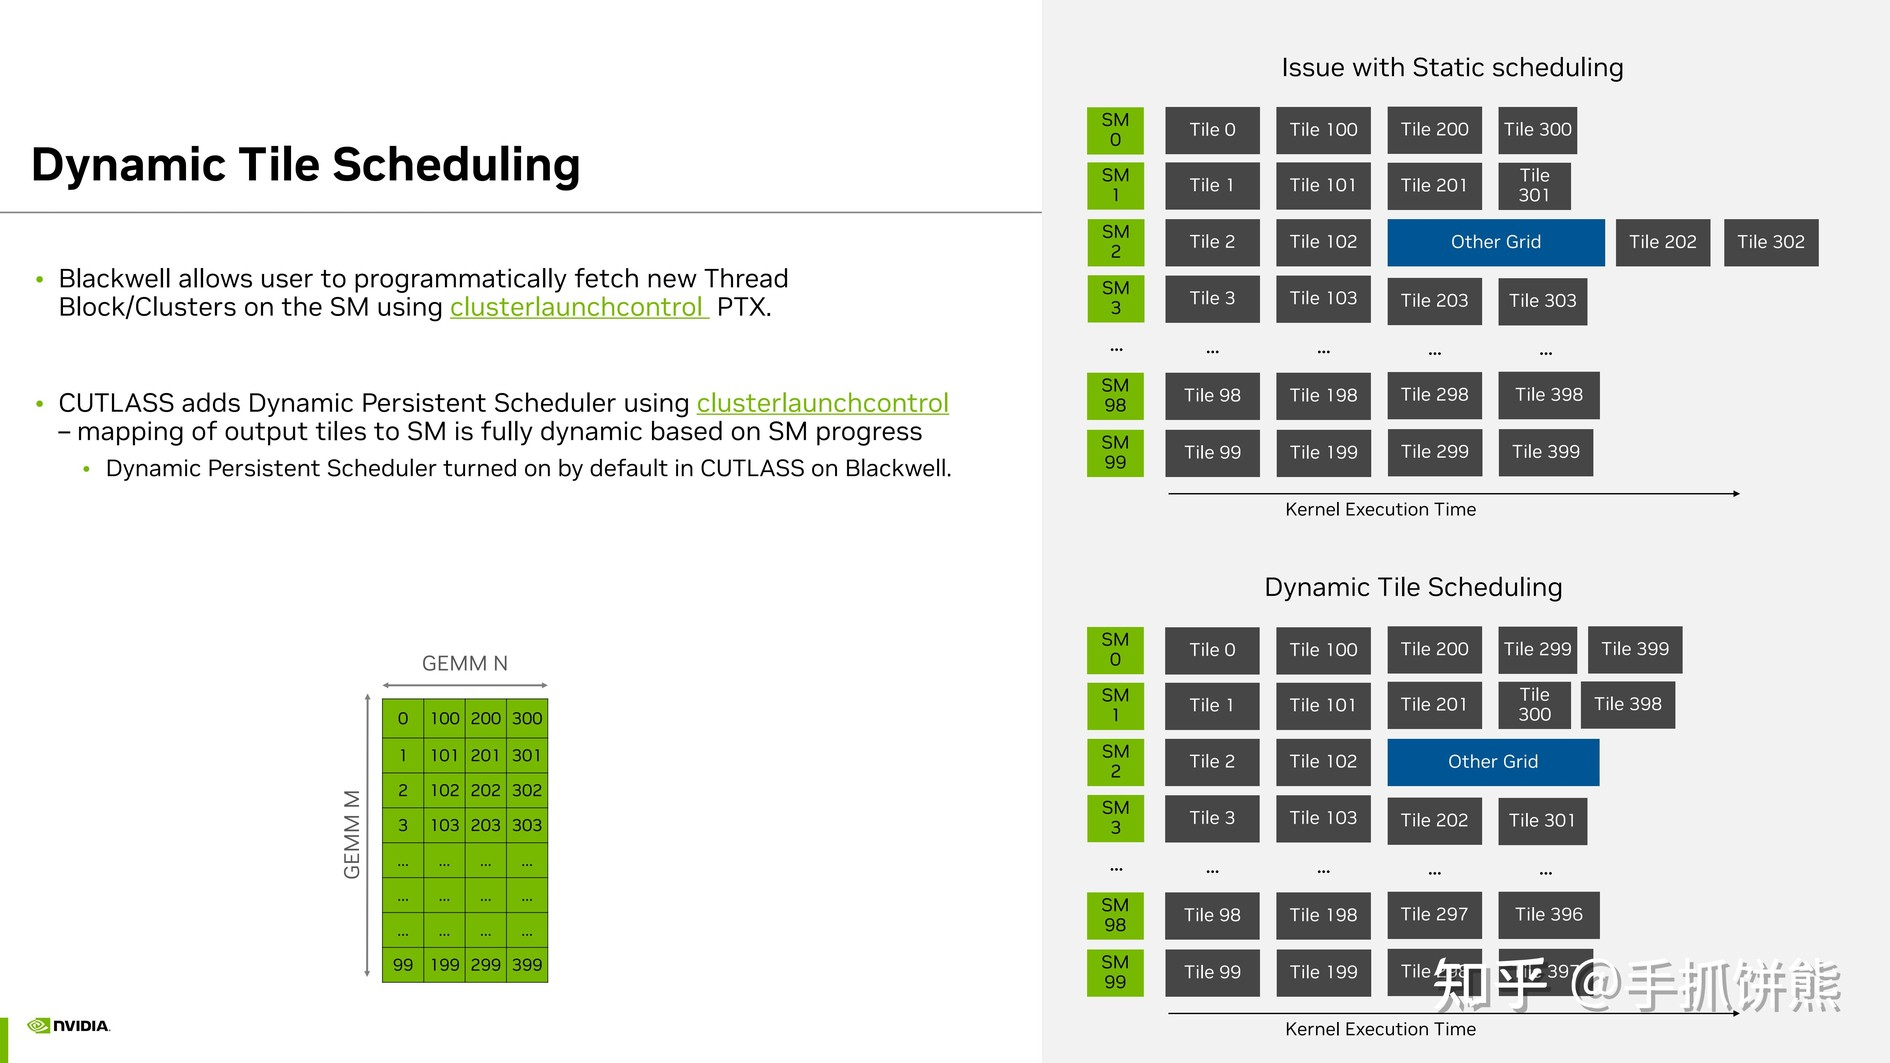
\includegraphics[width=0.9\textwidth]{figures/zhaoshangchun-01-tensor-core-programming/fig-13.jpg}
\end{figure}

针对静态调度的痛点，Blackwell 引入了\textbf{动态分块调度 (Dynamic Tile Scheduling)}。这得益于一个新的 PTX 指令 \texttt{clusterlaunchcontrol} (CLC)，它允许 SM 在运行时\textbf{主动向硬件请求新的工作单元}（Thread Block 或 Cluster）。基于此，CUTLASS 在 Blackwell 上实现了一个\textbf{动态持久调度器}（Dynamic Persistent Scheduler），并将其作为默认选项。

在这种新模式下，\textbf{输出 tile 与 SM 之间的映射不再是固定的}。任何一个 SM 在完成当前 tile 的计算后，都会\textbf{立即向调度器请求下一个尚未被处理的 tile}。如图右侧所示，即使 SM 1 被抢占，它回来后也只是像其他 SM 一样去请求新的任务。原来分配给它的 tile 201 和 301 可能会被其他空闲的 SM（如 SM 99）“认领”并完成。这种“能者多劳”的动态认领机制，\textbf{极大地平滑了因抢占或工作负载不均导致的长尾问题}，确保了所有 SM 都能持续保持忙碌，从而显著提升了 GPU 在复杂、多任务环境下的实际利用率和性能稳定性。

\textbf{第 14 页：Blackwell 架构新特性最终总结}

\begin{figure}[H]\centering
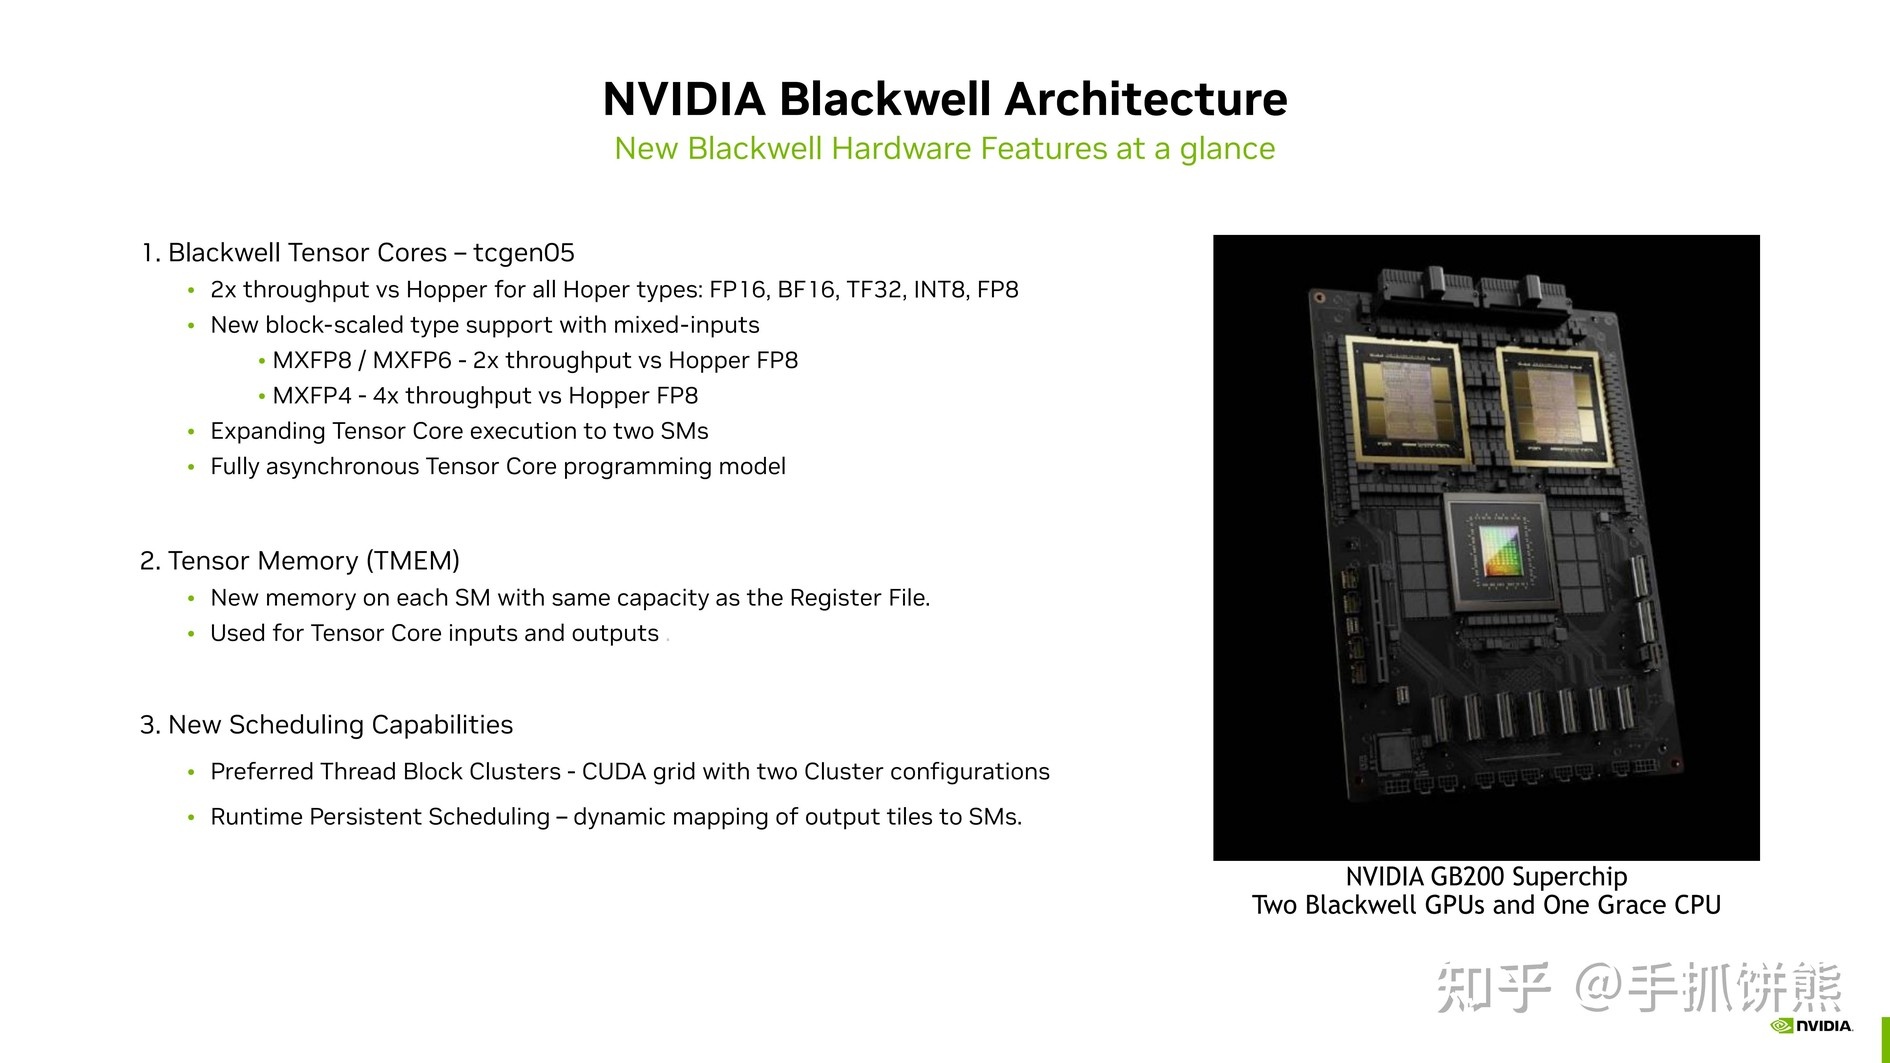
\includegraphics[width=0.9\textwidth]{figures/zhaoshangchun-01-tensor-core-programming/fig-14.jpg}
\end{figure}

这张总结性的幻灯片，将 Blackwell 架构的三大核心革新完整地串联了起来：

\begin{enumerate}
\item \textbf{第五代 Tensor Core (tcgen05)}：通过 2-SM-MMA、新低比特格式和全异步模型，实现了算力的巨大飞跃。
\item \textbf{Tensor Memory (TMEM)}：作为专用的片上张量内存，为 Tensor Core 提供了高速数据通道，是实现高性能计算的关键支撑。
\item \textbf{新的调度能力}：通过“首选线程块簇”和“动态持久调度”，解决了硬件资源碎片化和长尾效应问题，提升了 GPU 的实际利用率和鲁棒性。
\end{enumerate}

至此，我们对 Blackwell有了全面的了解。

\section{\textbf{三、使用 CuTe 驾驭 Blackwell 新特性}}

在了解了 Blackwell 新硬件特性之后，下一个核心问题是：我们如何在代码中利用它们？本章将聚焦于 \textbf{Cu\allowbreak{}Te}——CUTLASS 3.x 引入的底层张量抽象库。Cu\allowbreak{}Te 扮演着硬件与上层 CUTLASS 逻辑之间的桥梁，它将复杂的硬件指令、内存层级和线程协作模式，抽象为一套基于 C++ 模板的、富有表现力的“张量语言”。本章将通过一系列代码示例，展示 Cu\allowbreak{}Te 如何逐一解锁 Blackwell 的核心能力。

\subsection{\textbf{CuTe 核心抽象与 MMA 编程}}

本小节将介绍 Cu\allowbreak{}Te 的基石——MMA Atom 和 Tiled\allowbreak{}MMA，并通过一个完整的 GEMM 示例，展示如何用这些抽象来构建一个在 Blackwell 上运行的计算核心。

\textbf{第 15-16 页：CUTE 章节目录}

\begin{figure}[H]\centering
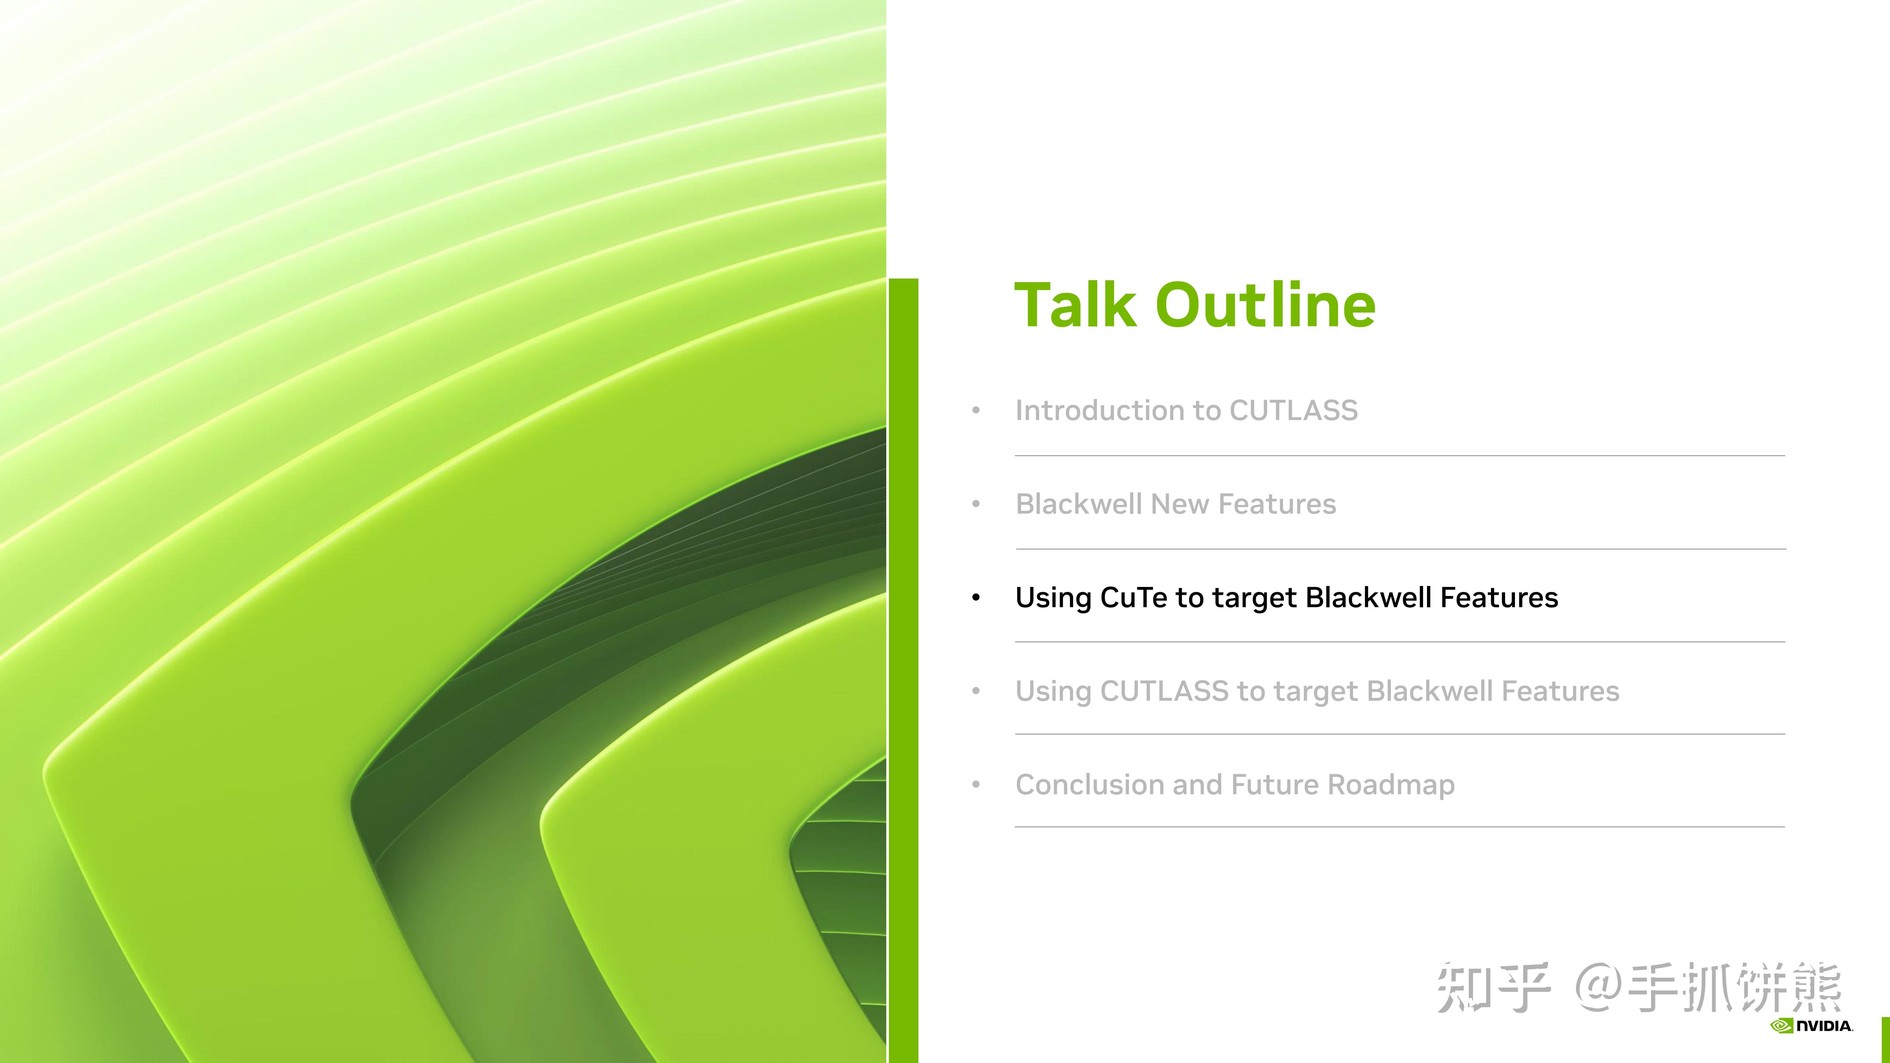
\includegraphics[width=0.9\textwidth]{figures/zhaoshangchun-01-tensor-core-programming/fig-15.jpg}
\end{figure}

\begin{figure}[H]\centering
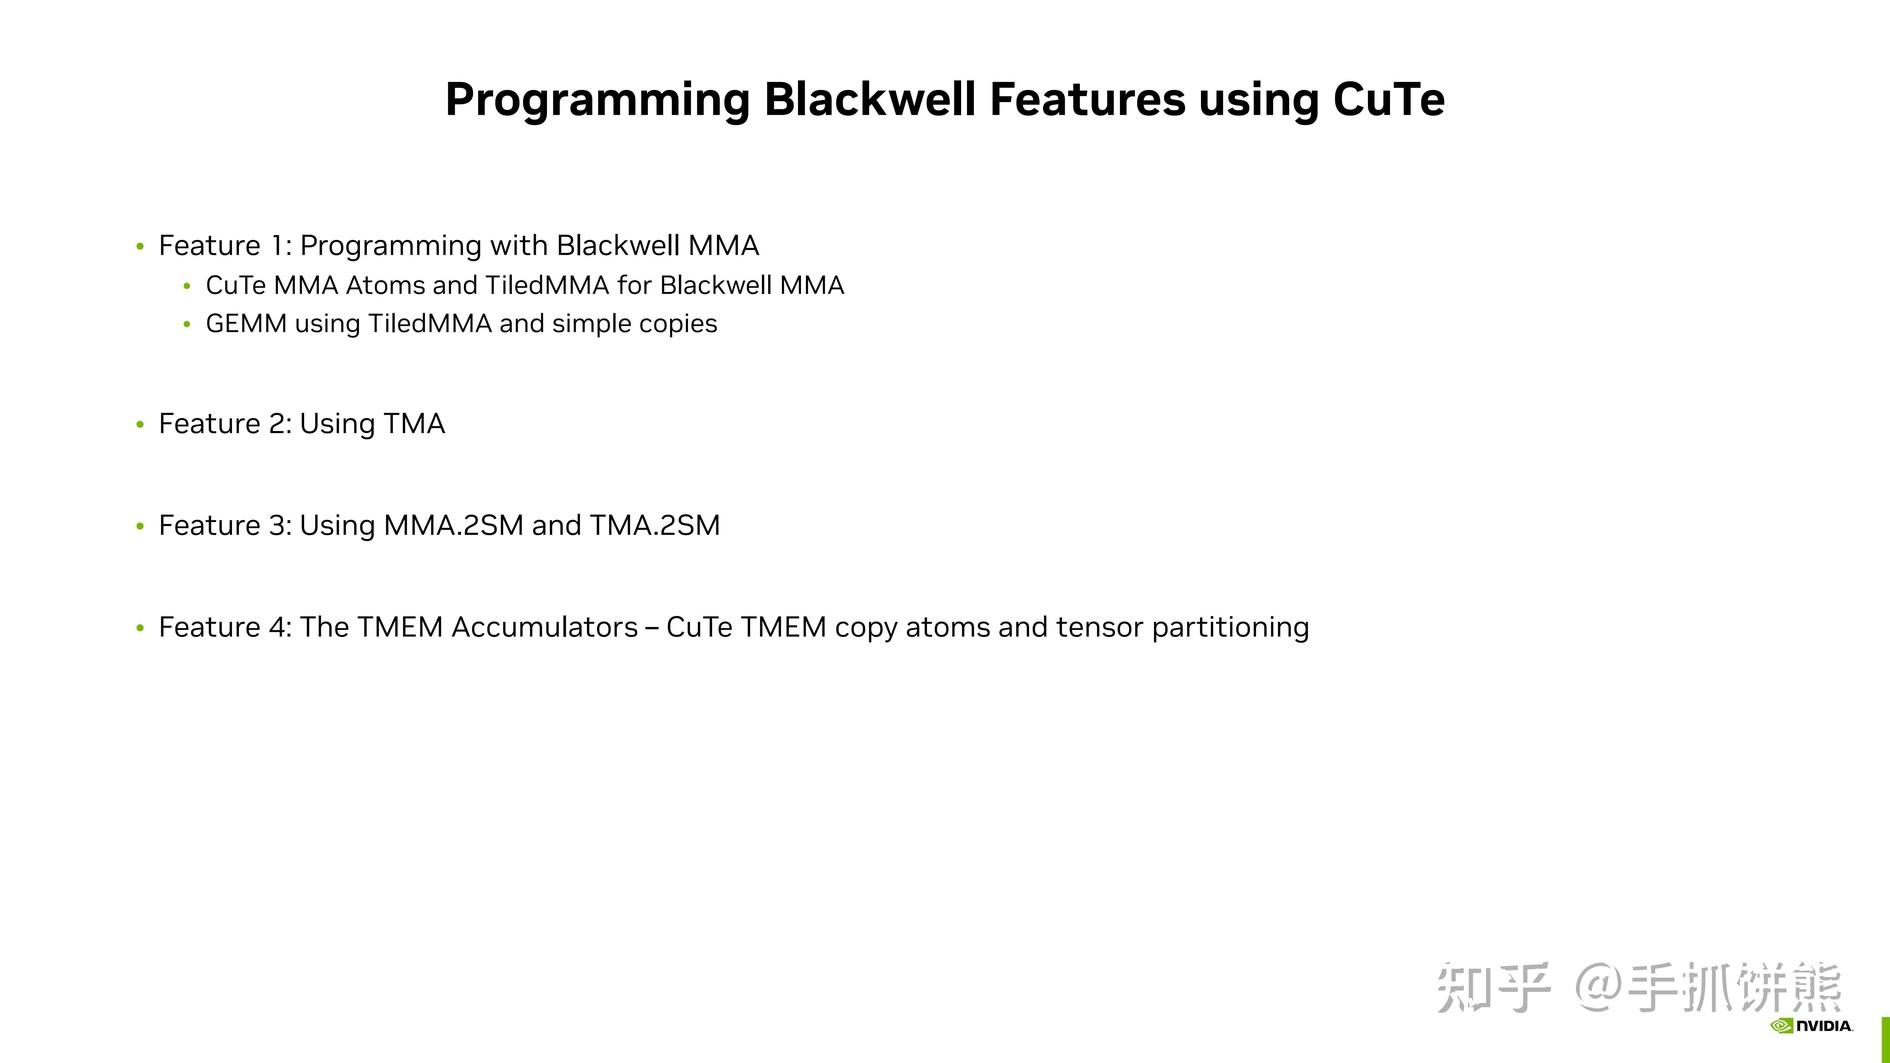
\includegraphics[width=0.9\textwidth]{figures/zhaoshangchun-01-tensor-core-programming/fig-16.jpg}
\end{figure}

这几页明确了本章的讨论重点，即使用 Cu\allowbreak{}Te 编程 Blackwell 的四个关键特性：

\begin{enumerate}
\item \textbf{编程 Blackwell MMA}：如何使用 Cu\allowbreak{}Te 的 MMA Atom 和 Tiled\allowbreak{}MMA 抽象来调用新的 \texttt{tcgen05.\allowbreak{}mma} 指令。
\item \textbf{使用 TMA}：如何利用 Cu\allowbreak{}Te 的抽象来发起异步内存传输。
\item \textbf{使用 MMA.2\allowbreak{}SM 和 TMA.2\allowbreak{}SM}：如何编程跨 SM 的 MMA 计算和数据加载。
\item \textbf{TMEM 累加器}：如何通过 Cu\allowbreak{}Te 的 TMEM copy atom 和张量分区来管理和操作位于 TMEM 中的累加器。
\end{enumerate}

这个目录清晰描述了本章的学习路径，从最基本的 MMA 计算开始，逐步引入异步数据加载、跨 SM 协作，最后到处理计算结果，覆盖了编写一个完整高性能核函数的全过程。

\textbf{第 17 页：使用 Cu\allowbreak{}Te 编程 Blackwell 特性（Tensor Core MMA部分）}

\begin{figure}[H]\centering
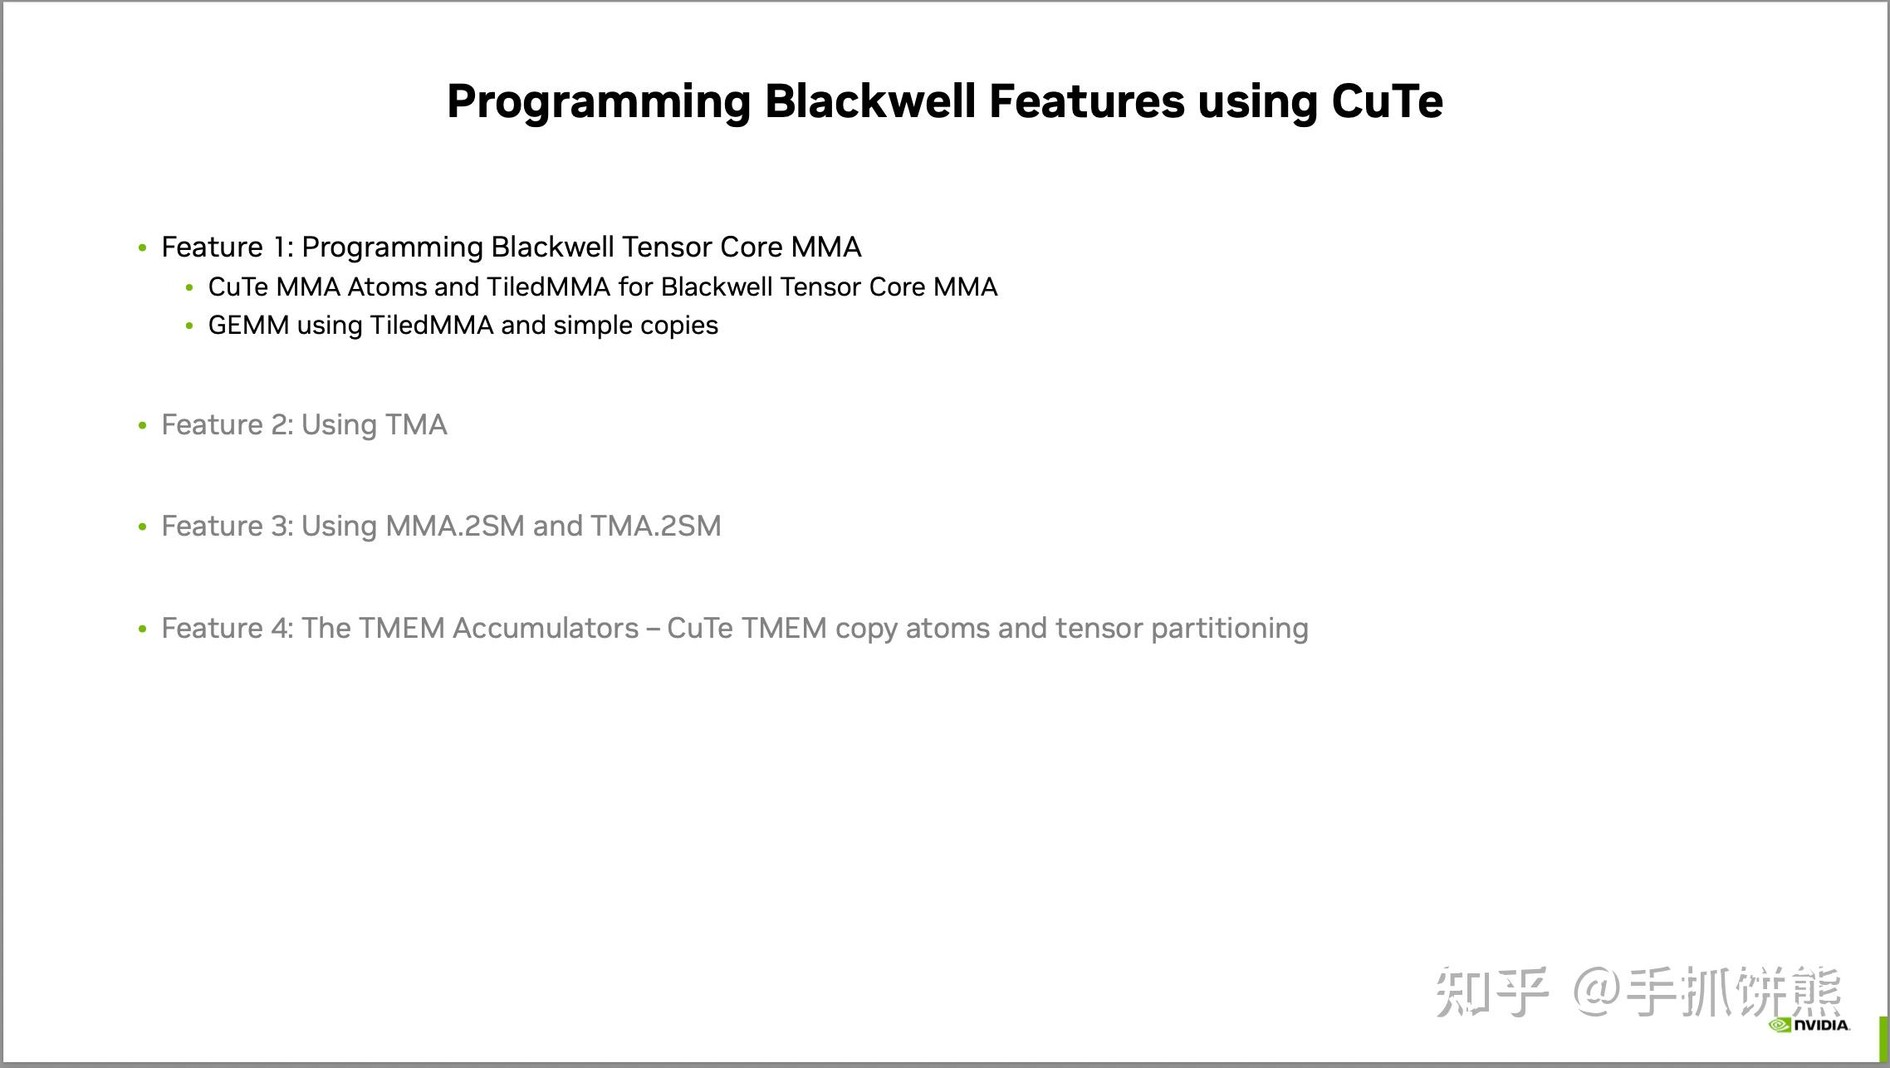
\includegraphics[width=0.9\textwidth]{figures/zhaoshangchun-01-tensor-core-programming/fig-17.jpg}
\end{figure}

从本页开始，随后 18-20 页，开始CUTE MMA和Tiled\allowbreak{}MMA的介绍。

\textbf{第 18：Cu\allowbreak{}Te MMA抽象}

\begin{figure}[H]\centering
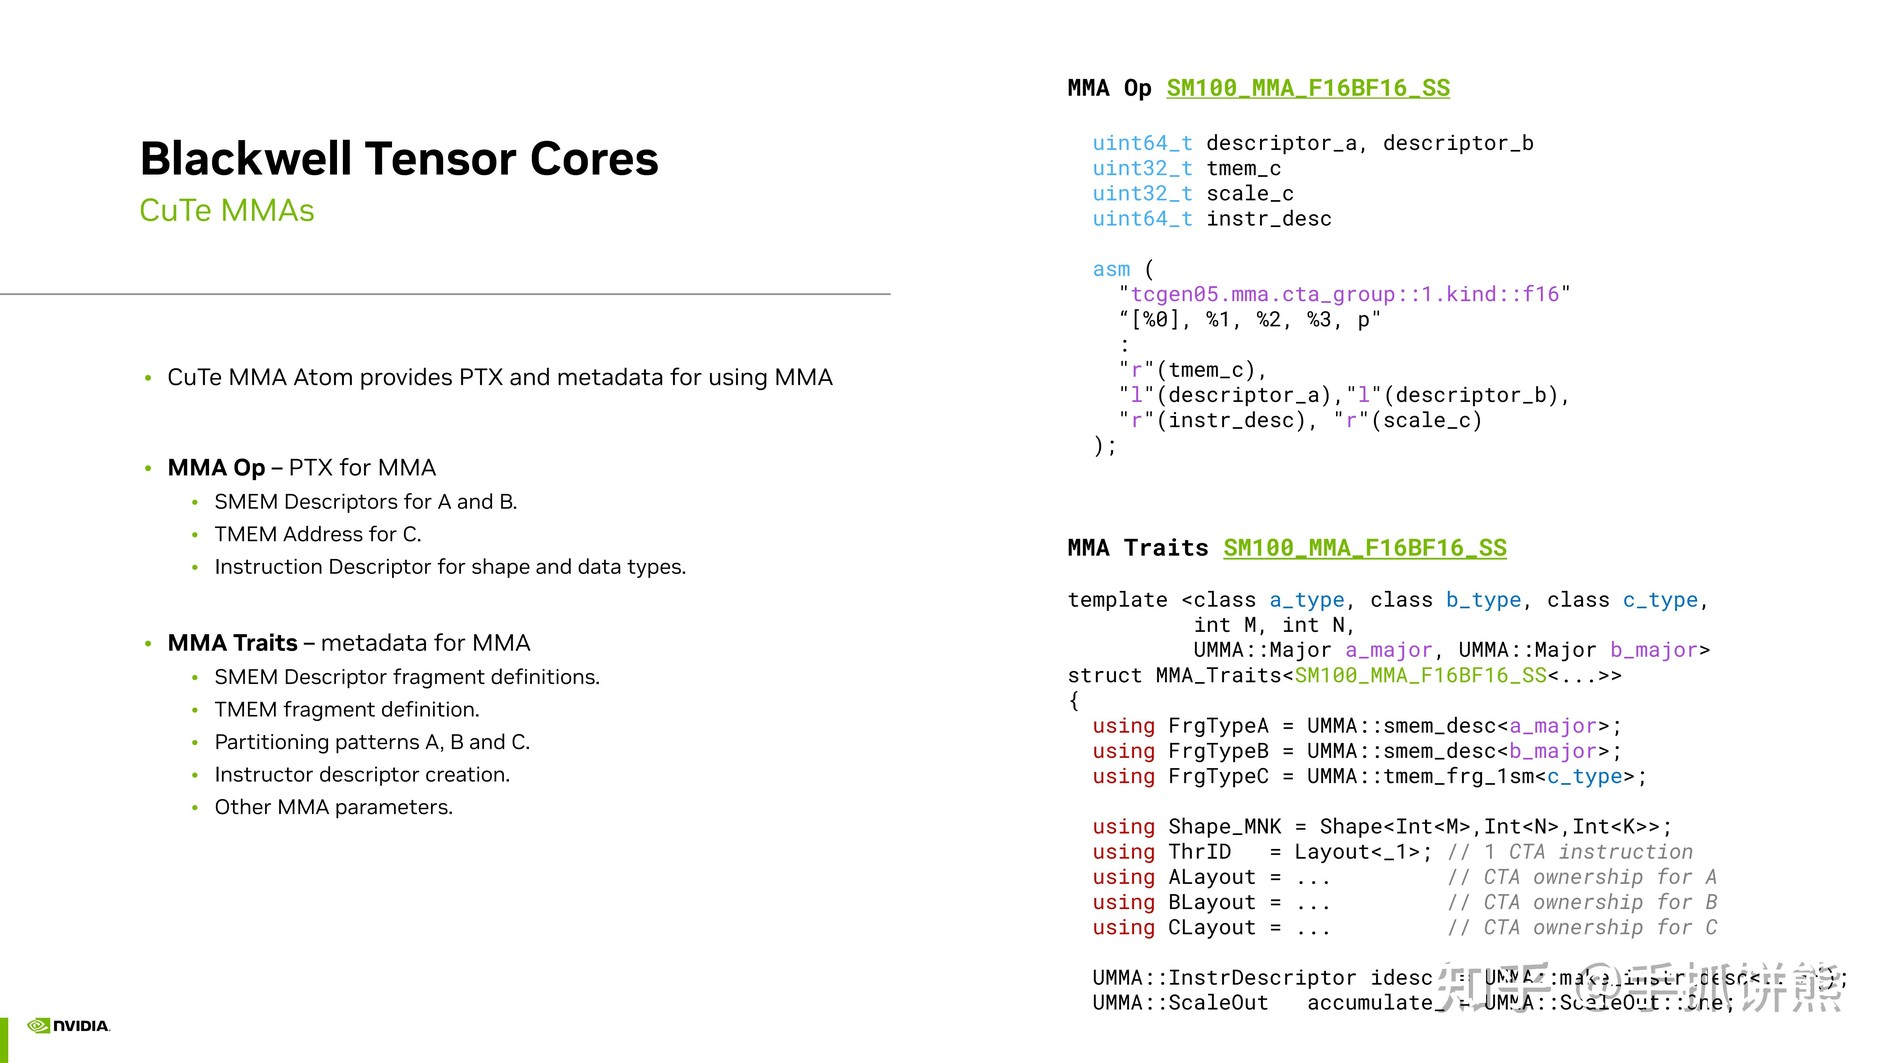
\includegraphics[width=0.9\textwidth]{figures/zhaoshangchun-01-tensor-core-programming/fig-18.jpg}
\end{figure}

第18页介绍了 Cu\allowbreak{}Te 对 MMA 指令的核心抽象：

\textbf{MMA Atom}。一个 MMA Atom 包含两部分：\textbf{MMA Op}，这是一个内联 PTX 汇编的封装，Blackwell架构直接对应硬件的 tcgen05.mma 指令，负责执行实际的计算；

\textbf{MMA Traits}，这是一个 C++ 模板元编程结构，包含了与该 MMA 指令相关的所有“元数据”，如数据分片定义、分区模式等。

\textbf{第 19 页：Blackwell和Hopper的MMA区别}

\begin{figure}[H]\centering
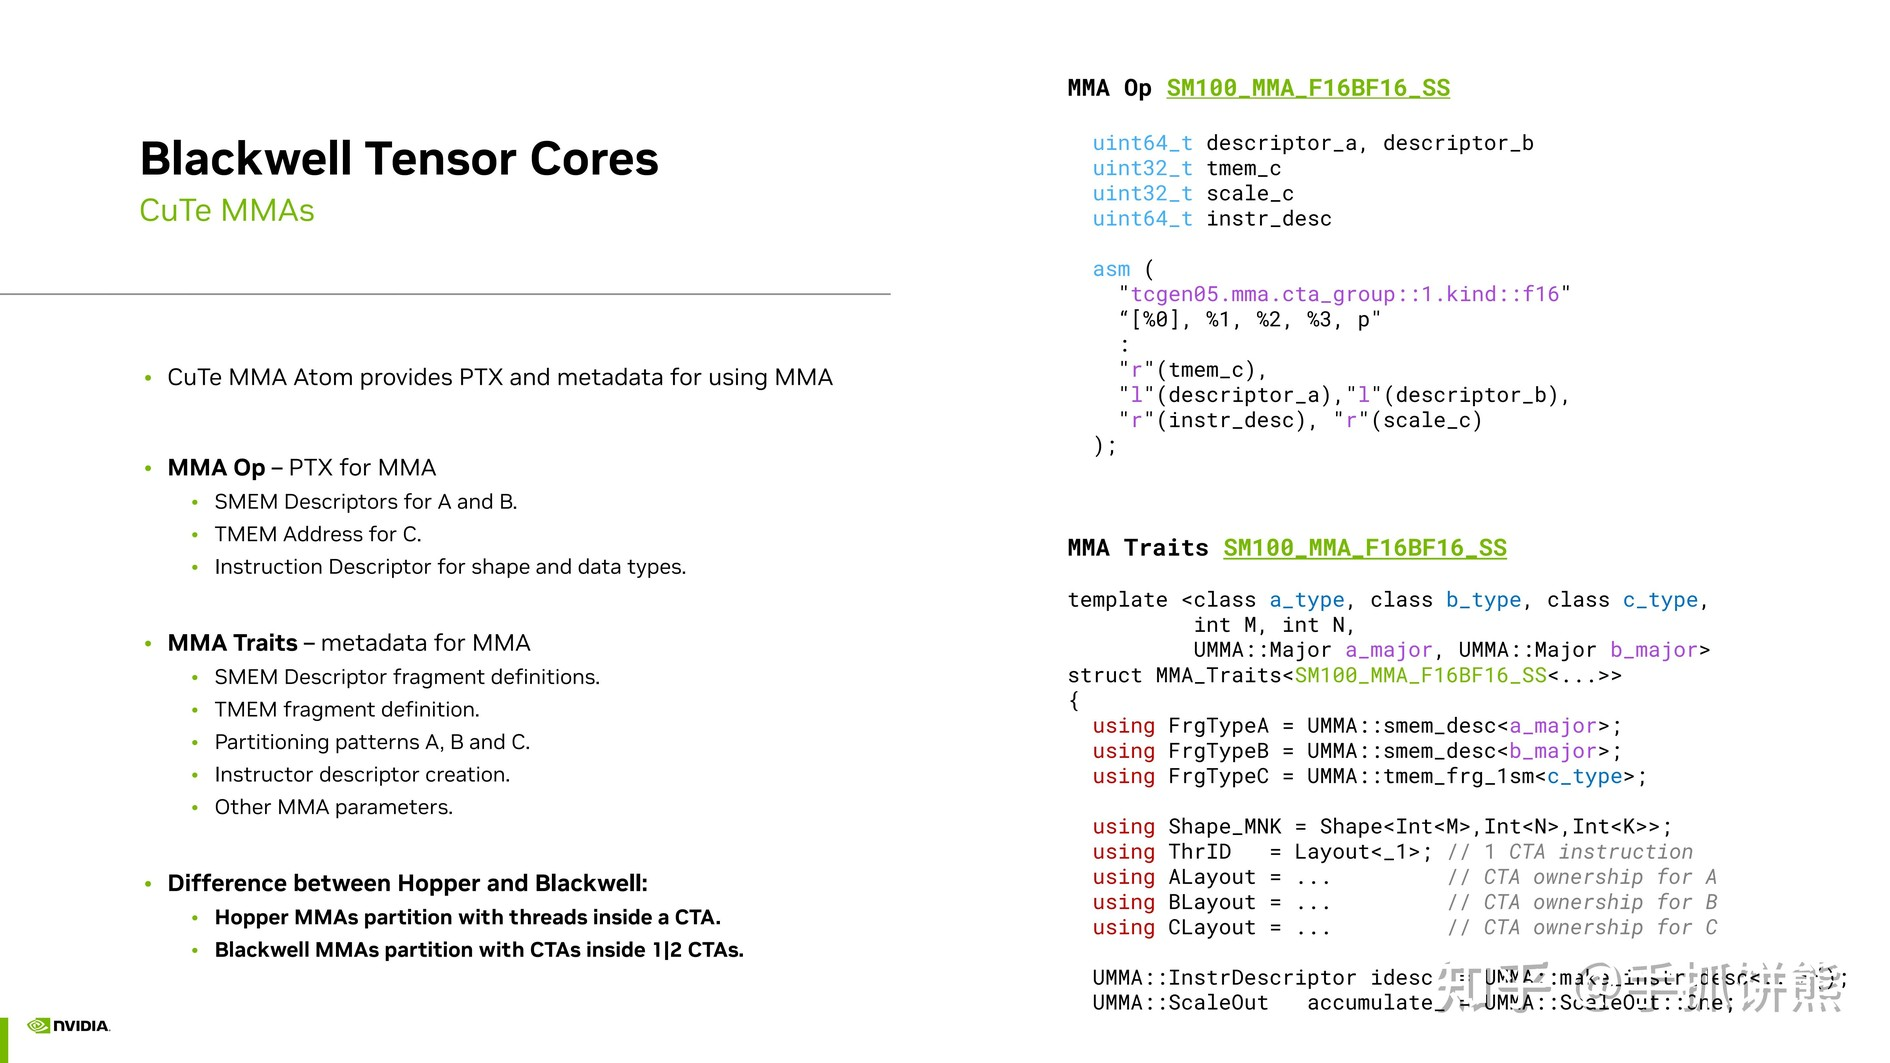
\includegraphics[width=0.9\textwidth]{figures/zhaoshangchun-01-tensor-core-programming/fig-19.jpg}
\end{figure}

第 19 页特别指出了 Blackwell MMA 与 Hopper 的一个\textbf{根本性区别}：Hopper 的 MMA 是在\textbf{一个 CTA 内部的线程之间}进行划分和协作的；而 Blackwell 的 MMA 则是在\textbf{一个或两个 CTA 之间}进行划分和协作。这个变化直接体现在 \texttt{MMA Traits} 的 \texttt{Thr\allowbreak{}ID} 定义上，它决定了指令的协作粒度。这种从 \texttt{thread-cooperative} 到 \texttt{CTA-cooperative} 的转变，是理解 Blackwell 编程模型演进的关键，它要求我们在更高的“集体”层面来思考和组织计算。

\textbf{第 20 页：Blackwell Tiled\allowbreak{}MMA}

\begin{figure}[H]\centering
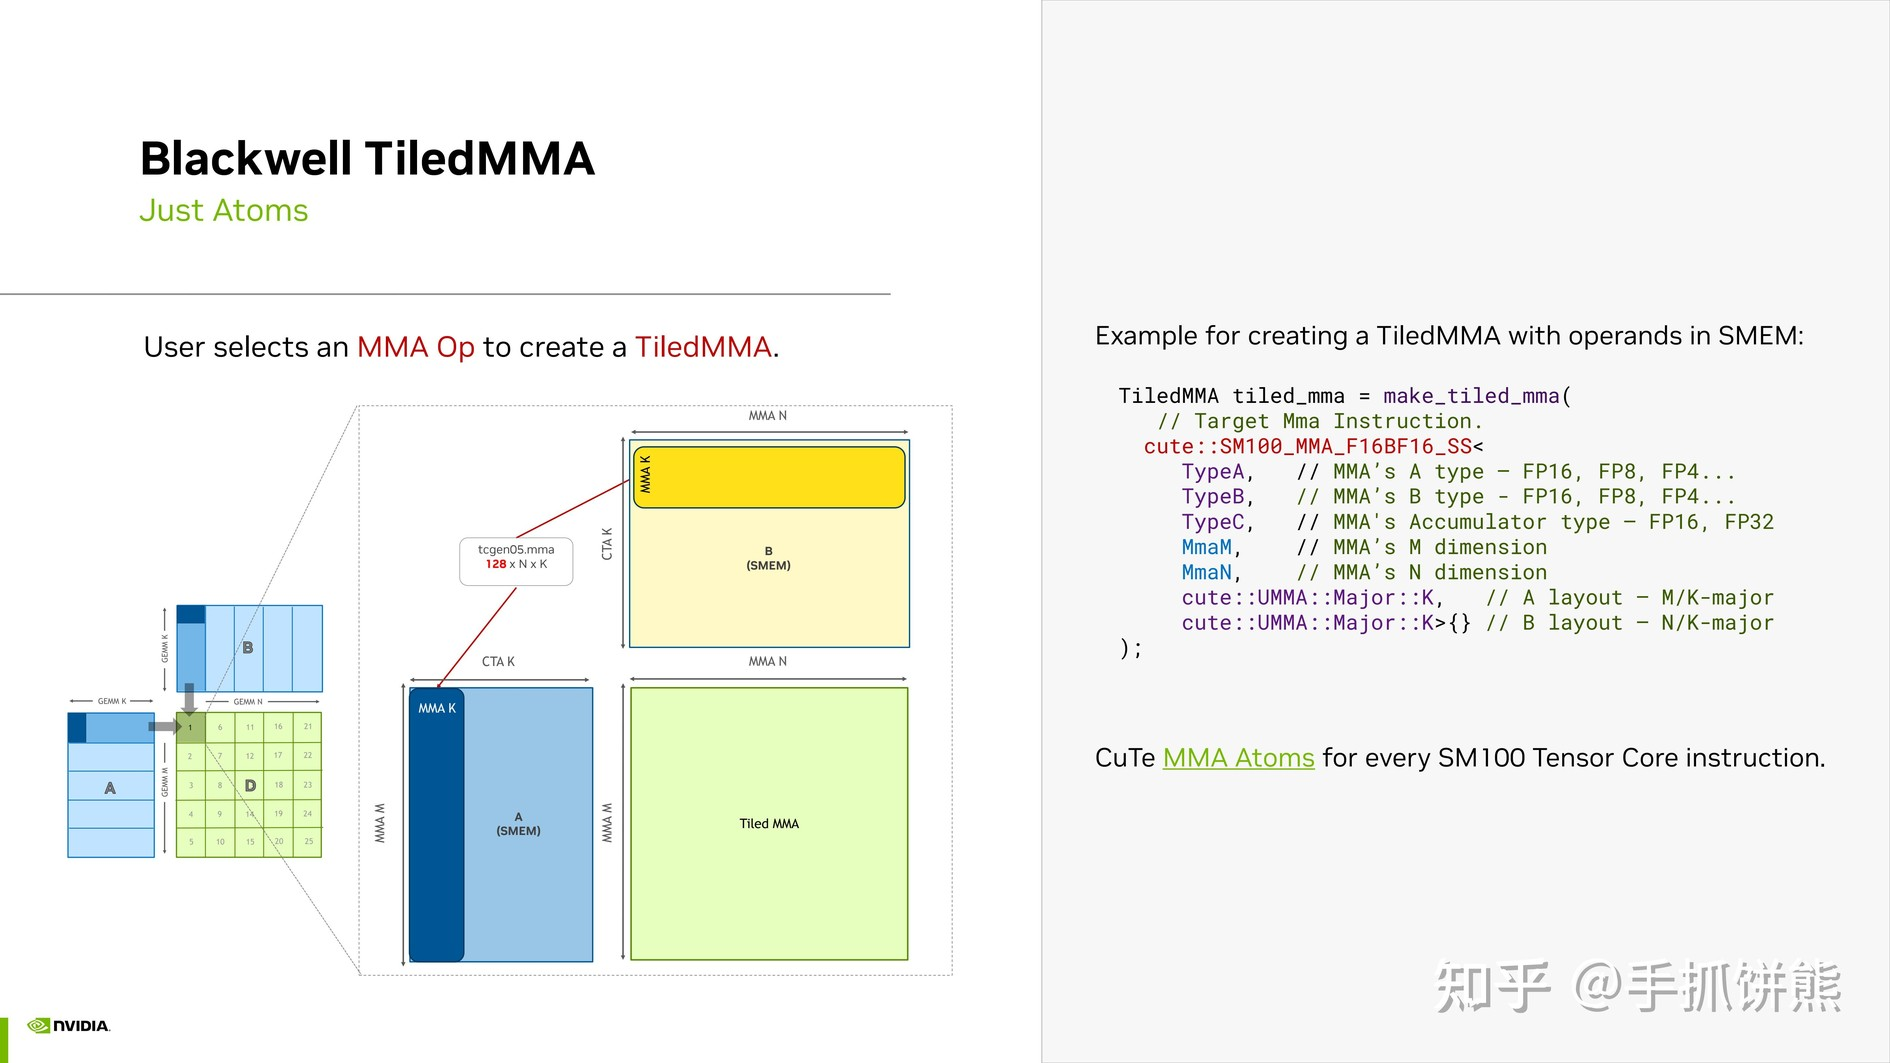
\includegraphics[width=0.9\textwidth]{figures/zhaoshangchun-01-tensor-core-programming/fig-20.jpg}
\end{figure}

在 \texttt{MMA Atom} 这一最底层的抽象之上，Cu\allowbreak{}Te 构建了 \textbf{Tiled\allowbreak{}MMA}。Tiled\allowbreak{}MMA 是一个更高层次的抽象，它将一个具体的 \texttt{MMA Atom} 在一个更大的 tile（分块）上进行“平铺”（tiling）。如图所示，一个大的 CTA tile 是由多个小的 \texttt{MMA Atom} tile 构成的。\texttt{make\_\allowbreak{}tiled\_\allowbreak{}mma} 工厂函数允许开发者通过指定目标 MMA 指令、数据类型、MMA 形状等，来方便地构建一个 Tiled\allowbreak{}MMA 对象。

Tiled\allowbreak{}MMA 将程序员从繁琐的循环和地址计算中解放出来。开发者只需要定义好宏观的计算任务（在一个大的 tile 上的 GEMM），Tiled\allowbreak{}MMA 就会自动处理如何将其分解为硬件支持的微观 MMA 指令序列。这是 Cu\allowbreak{}Te 实现“硬件无关性”和“代码可重用性”的核心机制，也是我们能够高效编写复杂核函数的基础。

\subsection{\textbf{Blackwell MMA GEMM 示例}}

\textbf{第 21-28 页，描述了一个完整的 Blackwell MMA GEMM 示例，}这一系列幻灯片通过一个名为 \texttt{01\_\allowbreak{}mma\_\allowbreak{}sm100.\allowbreak{}cu} 的示例，一步步地展示了如何使用 Cu\allowbreak{}Te 的组件从零开始构建一个在 Blackwell 上运行的 GEMM 核函数。

\textbf{第 21 页：定义全局内存张量 (Global Memory Tensors)}

\begin{figure}[H]\centering
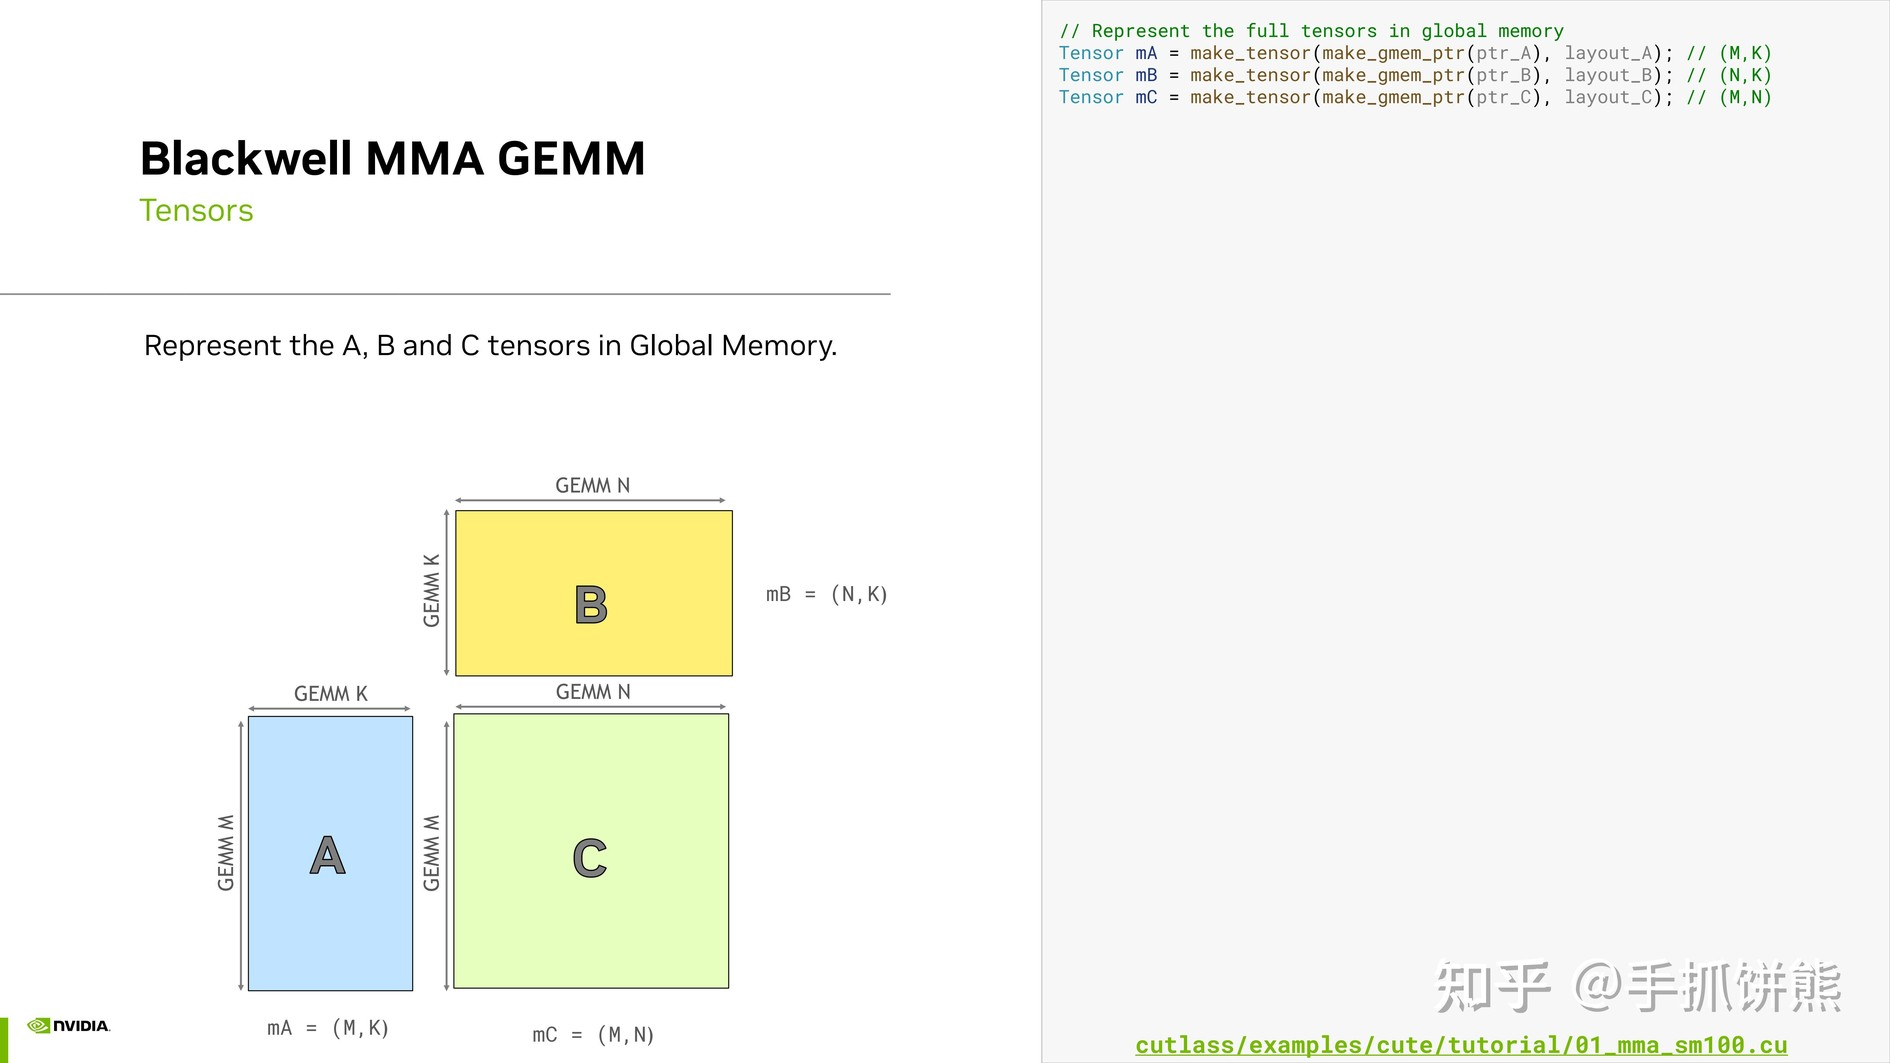
\includegraphics[width=0.9\textwidth]{figures/zhaoshangchun-01-tensor-core-programming/fig-21.jpg}
\end{figure}

Cu\allowbreak{}Te 使用 \texttt{make\_\allowbreak{}tensor} 函数，传入一个指向全局内存的指针和描述其形状与步长的 \texttt{layout}，来创建一个 \texttt{Tensor} 对象。这是对原始内存的第一次抽象。

\textbf{第 22-23 页：创建 MMA 分块视图 (MMA Tiler)}

\begin{figure}[H]\centering
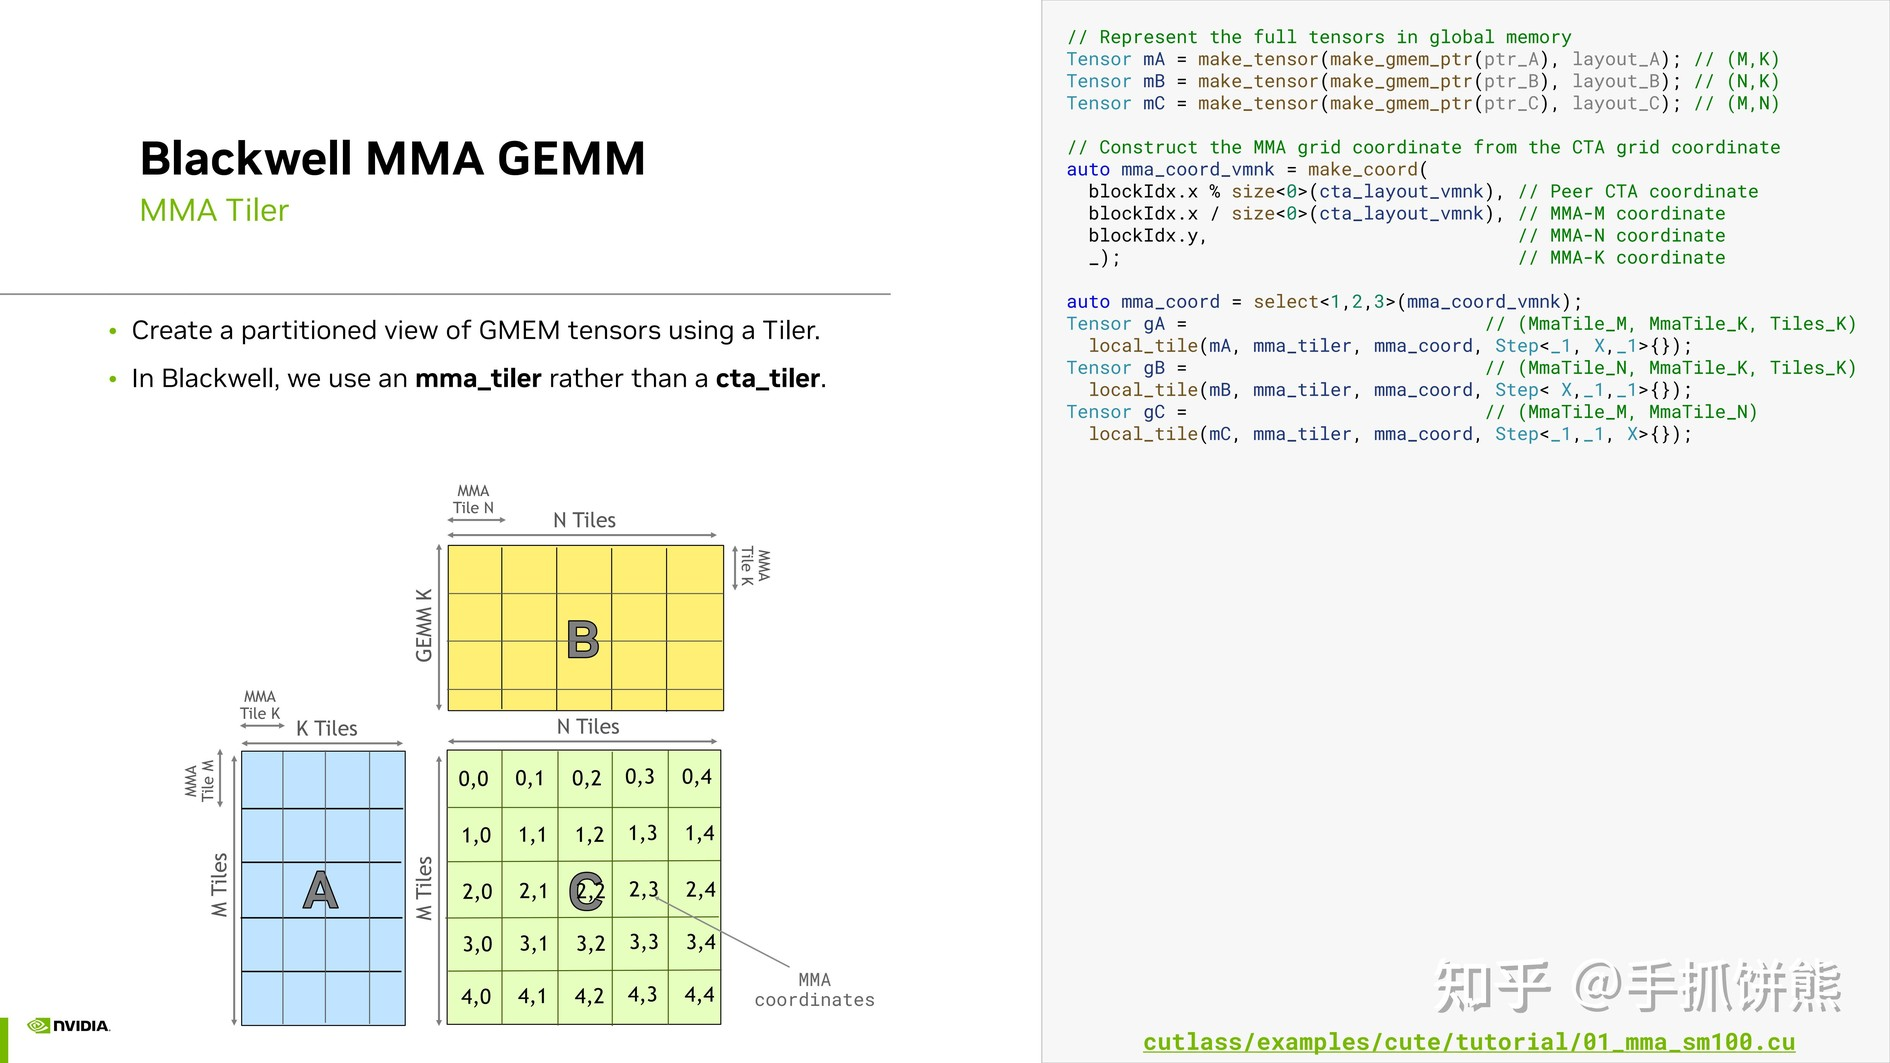
\includegraphics[width=0.9\textwidth]{figures/zhaoshangchun-01-tensor-core-programming/fig-22.jpg}
\end{figure}

\begin{figure}[H]\centering
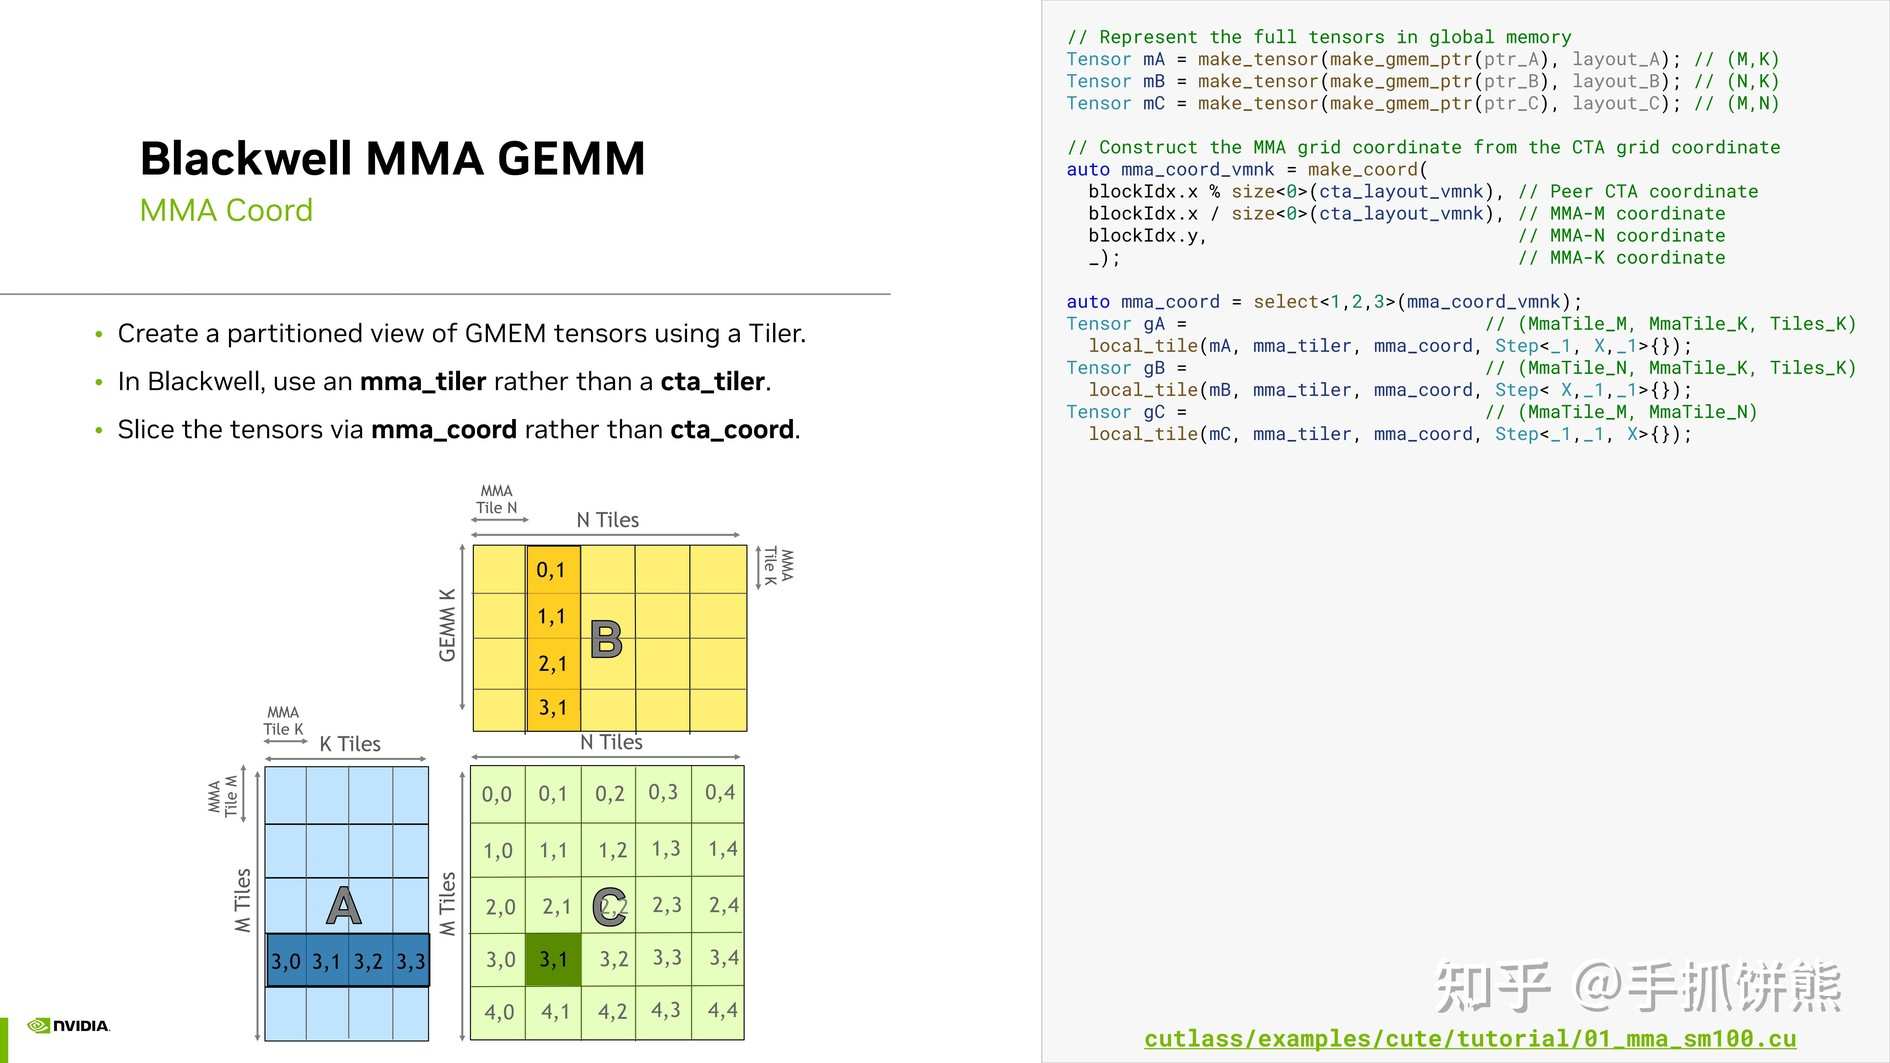
\includegraphics[width=0.9\textwidth]{figures/zhaoshangchun-01-tensor-core-programming/fig-23.jpg}
\end{figure}

与 Hopper 中基于 \texttt{cta\_\allowbreak{}tiler} 的做法不同，Blackwell 的编程模型引入了 \texttt{mma\_\allowbreak{}tiler}。\texttt{mma\_\allowbreak{}tiler} 负责将整个 GEMM 问题划分为一系列 MMA-tile。然后，通过 \texttt{local\_\allowbreak{}tile} 函数，并传入当前 CTA 对应的 \texttt{mma\_\allowbreak{}coord}，我们可以得到一个\textbf{只关注当前 MMA-tile 的局部张量视图}。这里的关键转变是，调度的基本单元从 CTA-tile 变成了 MMA-tile，这与 \textbf{Blackwell 的跨 SM 执行能力紧密相关}。

\textbf{第 24 页：在 MMA-tile 内部进行分区 (MMA Partitioning)}

\begin{figure}[H]\centering
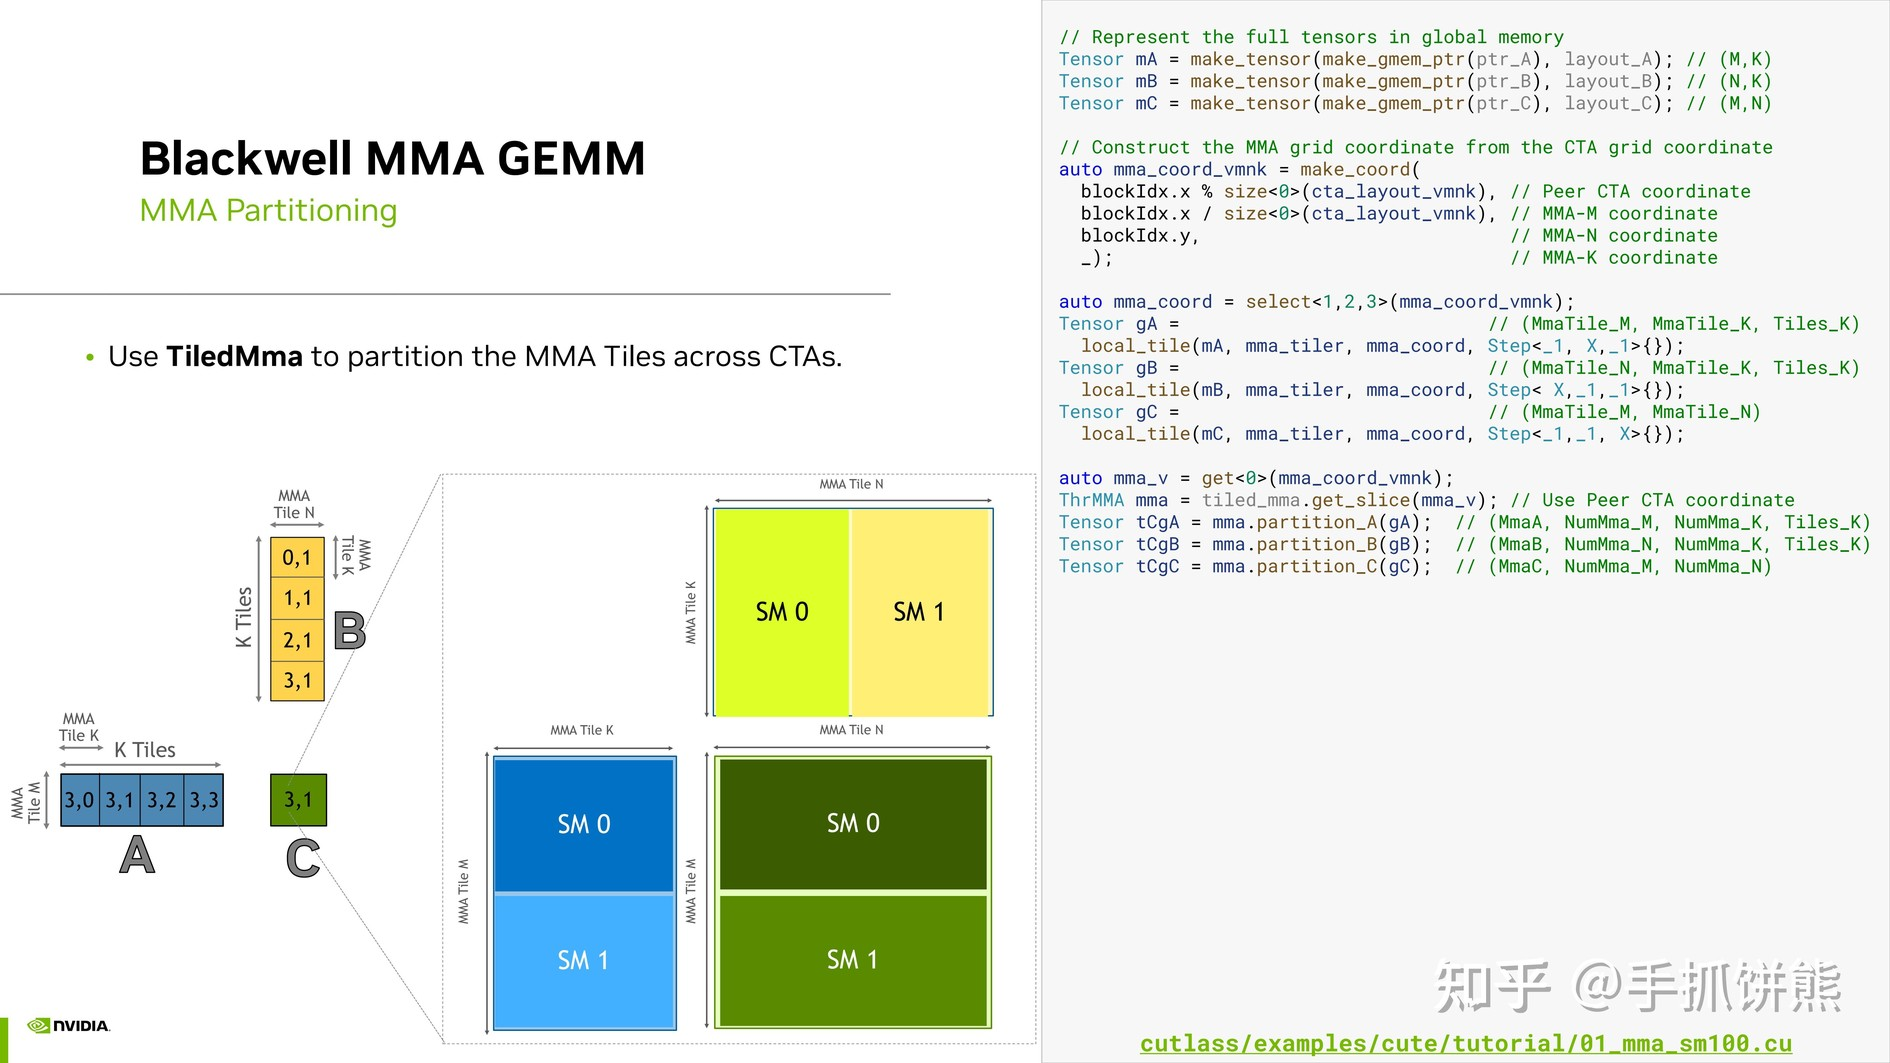
\includegraphics[width=0.9\textwidth]{figures/zhaoshangchun-01-tensor-core-programming/fig-24.jpg}
\end{figure}

获取了 MMA-tile 的视图后，下一步是利用 \texttt{Tiled\allowbreak{}MMA} 对象对其进行\textbf{分区}。\texttt{t\allowbreak{}i\allowbreak{}l\allowbreak{}e\allowbreak{}d\allowbreak{}\_\allowbreak{}m\allowbreak{}m\allowbreak{}a\allowbreak{}.\allowbreak{}g\allowbreak{}e\allowbreak{}t\allowbreak{}\_\allowbreak{}s\allowbreak{}l\allowbreak{}i\allowbreak{}c\allowbreak{}e\allowbreak{}(\allowbreak{}m\allowbreak{}m\allowbreak{}a\allowbreak{}\_\allowbreak{}v\allowbreak{})} 会根据当前 CTA 在一个 2-SM-MMA pair 中的角色返回对应的 \texttt{Thr\allowbreak{}MMA} 对象。然后，调用 \texttt{mma.\allowbreak{}partition\_\allowbreak{}A/\allowbreak{}B/\allowbreak{}C}，将 MMA-tile 视图进一步划分为当前 CTA \textbf{本地负责}的部分。如图右下角所示，原本一个完整的 \texttt{Mma\allowbreak{}Tile} 被均匀地划分到了 SM 0 和 SM 1 上。

\textbf{第 25 页：定义和分配共享内存 (SMEM)}

\begin{figure}[H]\centering
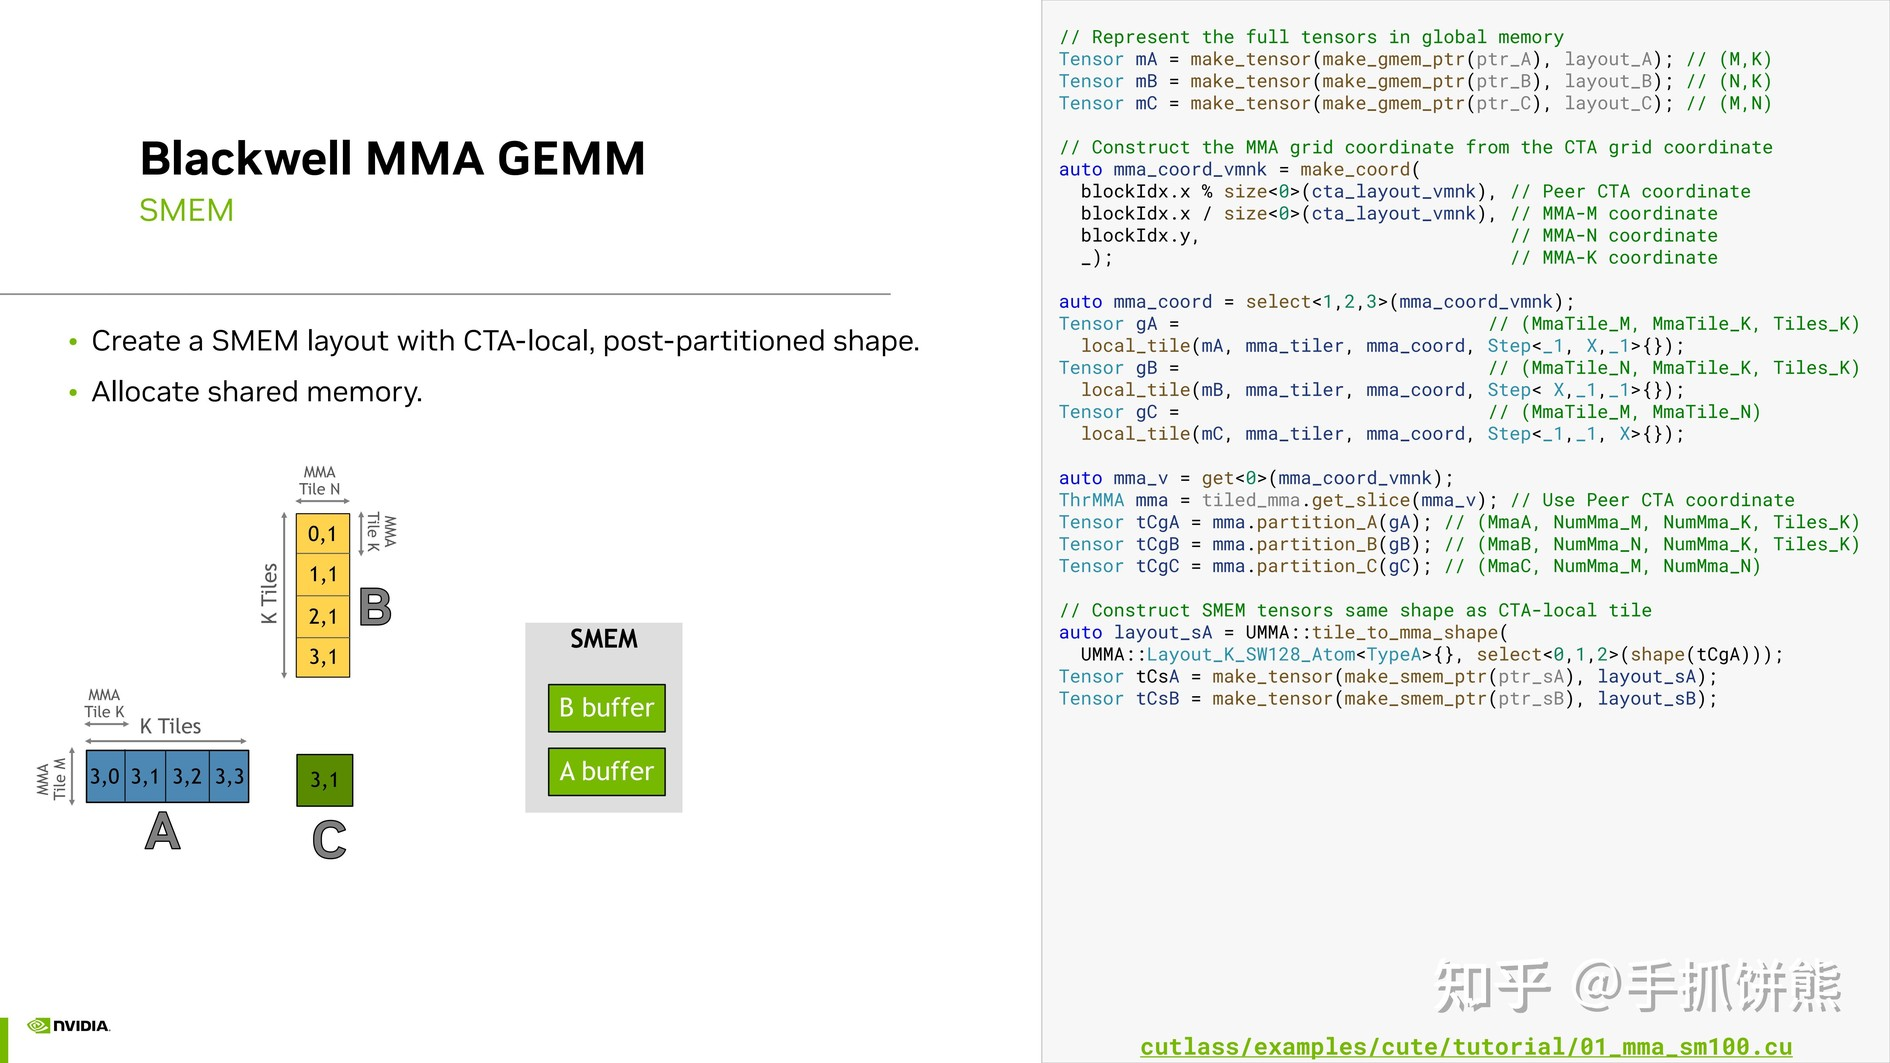
\includegraphics[width=0.9\textwidth]{figures/zhaoshangchun-01-tensor-core-programming/fig-25.jpg}
\end{figure}

有了 CTA 本地的数据视图，我们就可以为其在 SMEM 中分配缓冲区了。Cu\allowbreak{}Te 提供了 \texttt{UMMA::\allowbreak{}tile\_\allowbreak{}to\_\allowbreak{}mma\_\allowbreak{}shape} 等工具函数来帮助我们创建符合 MMA 指令要求的、经过优化的 SMEM 布局，以减少 bank conflict。然后，使用 \texttt{make\_\allowbreak{}tensor} 和 \texttt{make\_\allowbreak{}smem\_\allowbreak{}ptr} 即可创建 SMEM 张量。

\textbf{第 26 页：创建 MMA 片段 (Fragments)}

\begin{figure}[H]\centering
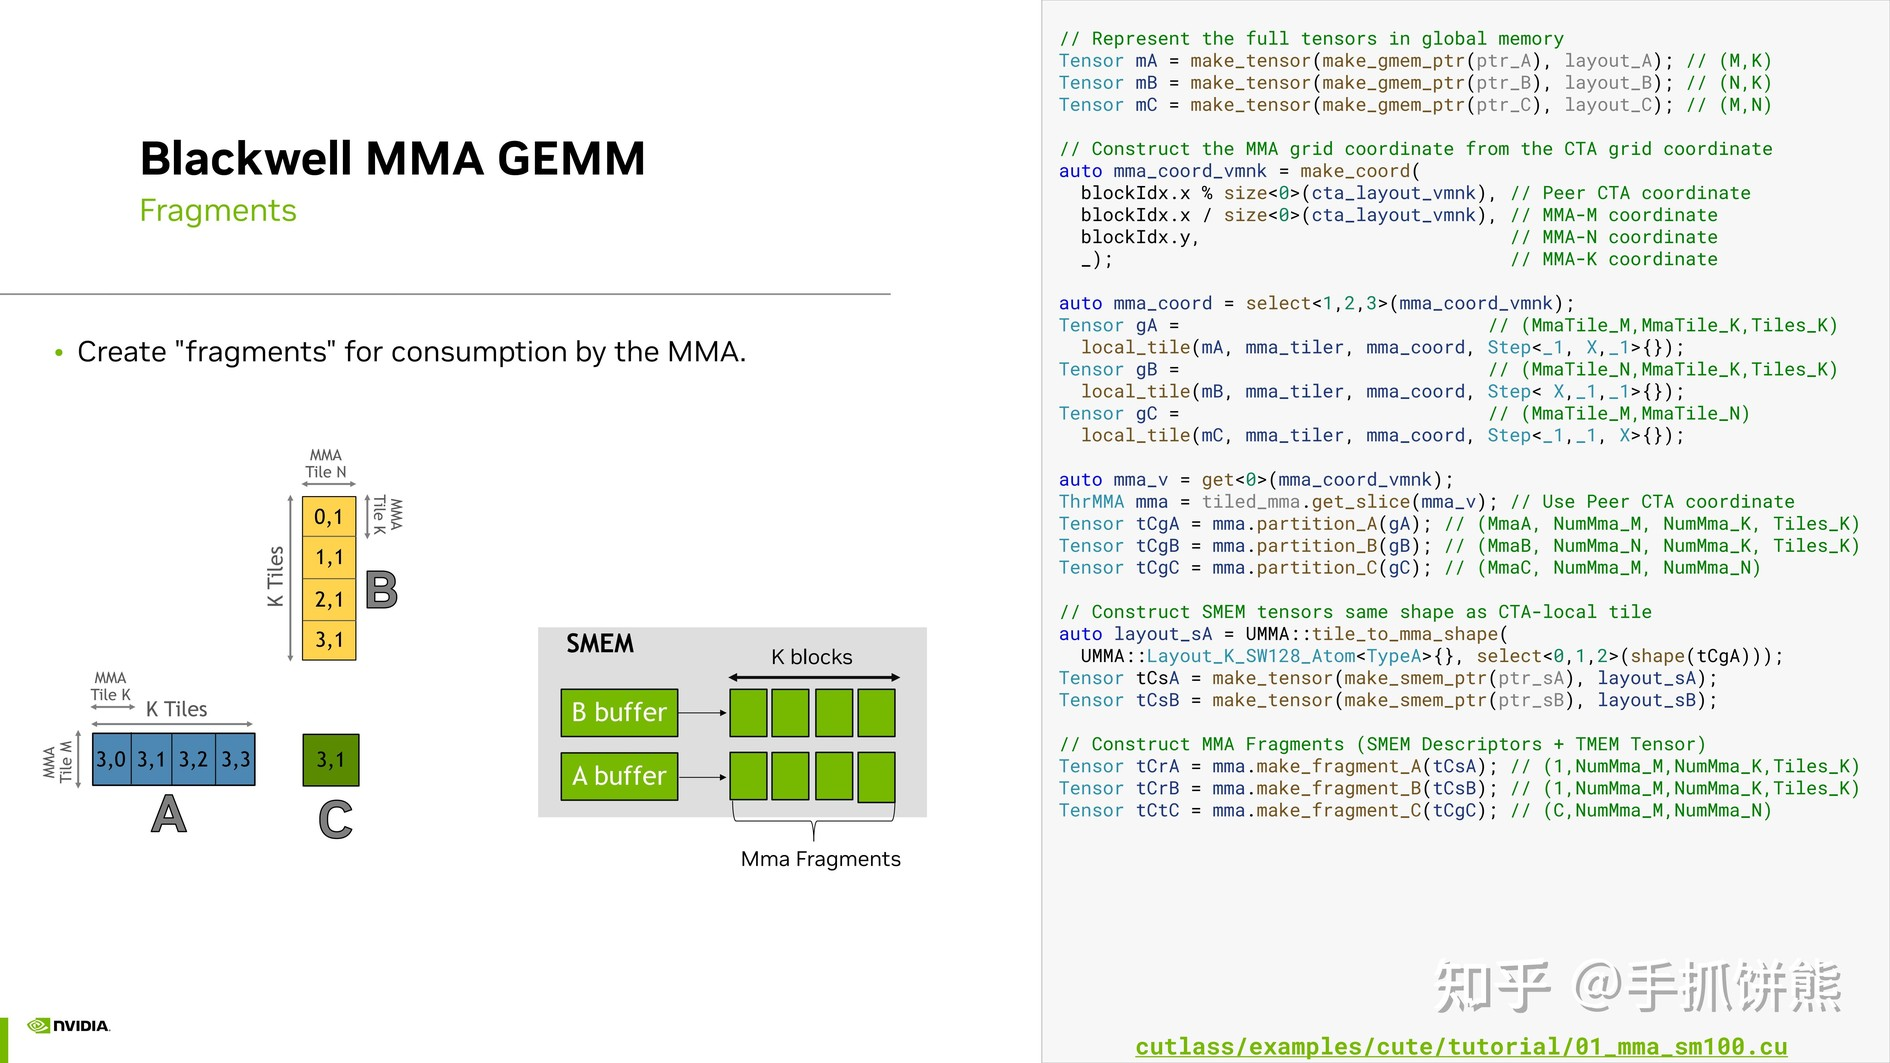
\includegraphics[width=0.9\textwidth]{figures/zhaoshangchun-01-tensor-core-programming/fig-26.jpg}
\end{figure}

“Fragment”是 Cu\allowbreak{}Te 中一个非常重要的概念，它代表了\textbf{一次 MMA 指令能够直接消费的数据单元}。调用 \texttt{mma.\allowbreak{}make\_\allowbreak{}fragment\_\allowbreak{}A/\allowbreak{}B/\allowbreak{}C} 会生成这些 fragments。对于输入 A 和 B，fragment 本质上是一个封装了 SMEM 地址的\textbf{描述符}。对于输出 C，由于它直接存在于 TMEM 中，fragment 就是一个指向 TMEM 的\textbf{张量对象}。

\textbf{第 27 页：从 GMEM 拷贝到 SMEM}

\begin{figure}[H]\centering
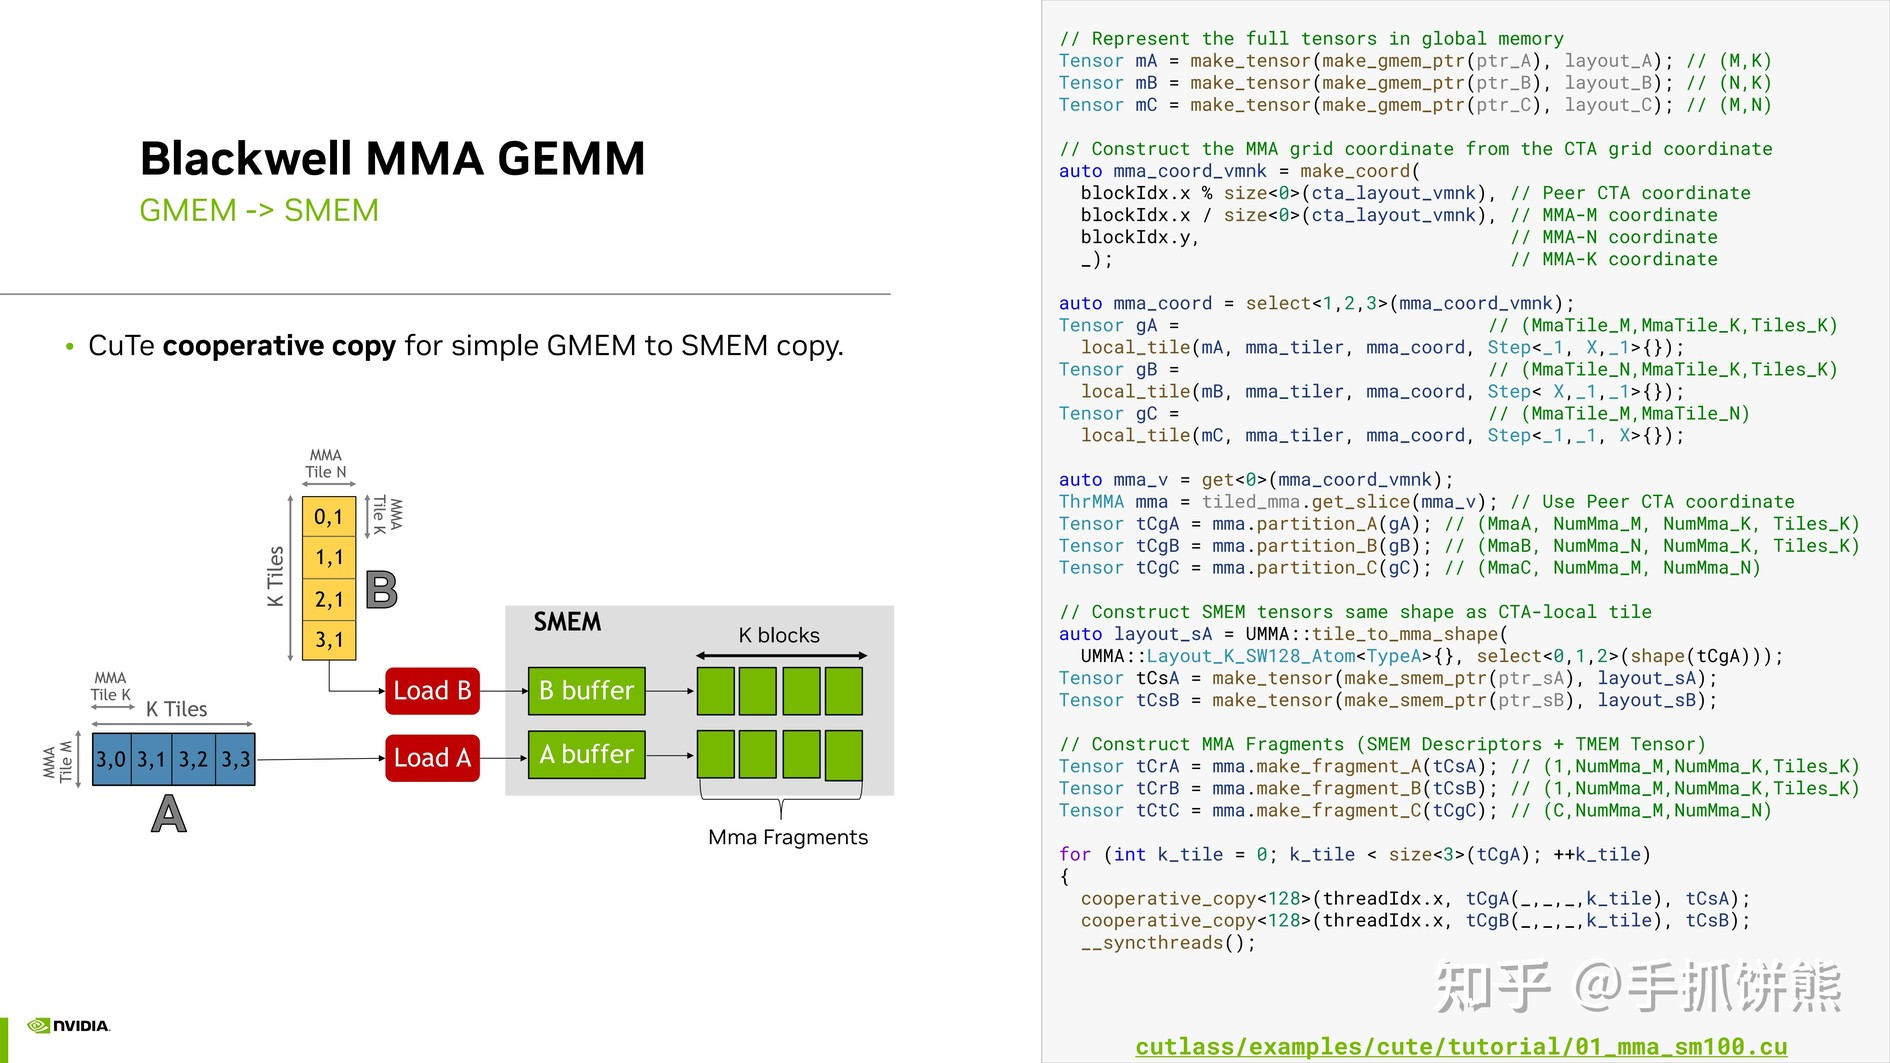
\includegraphics[width=0.9\textwidth]{figures/zhaoshangchun-01-tensor-core-programming/fig-27.jpg}
\end{figure}

在计算开始前，我们需要将 GMEM 中的数据搬运到 SMEM 中。这里使用了 \texttt{cooperative\_\allowbreak{}copy}，这是一个 CTA 内部所有线程协同工作的数据搬运原语。通过在一个 k-tile 循环中不断地拷贝数据，我们实现了经典的 mainloop 结构。\texttt{\_\allowbreak{}\_\allowbreak{}syncthreads()} 保证了在 SMEM 数据准备好之前，计算不会开始。

\textbf{第 28 页：执行 GEMM 计算}

\begin{figure}[H]\centering
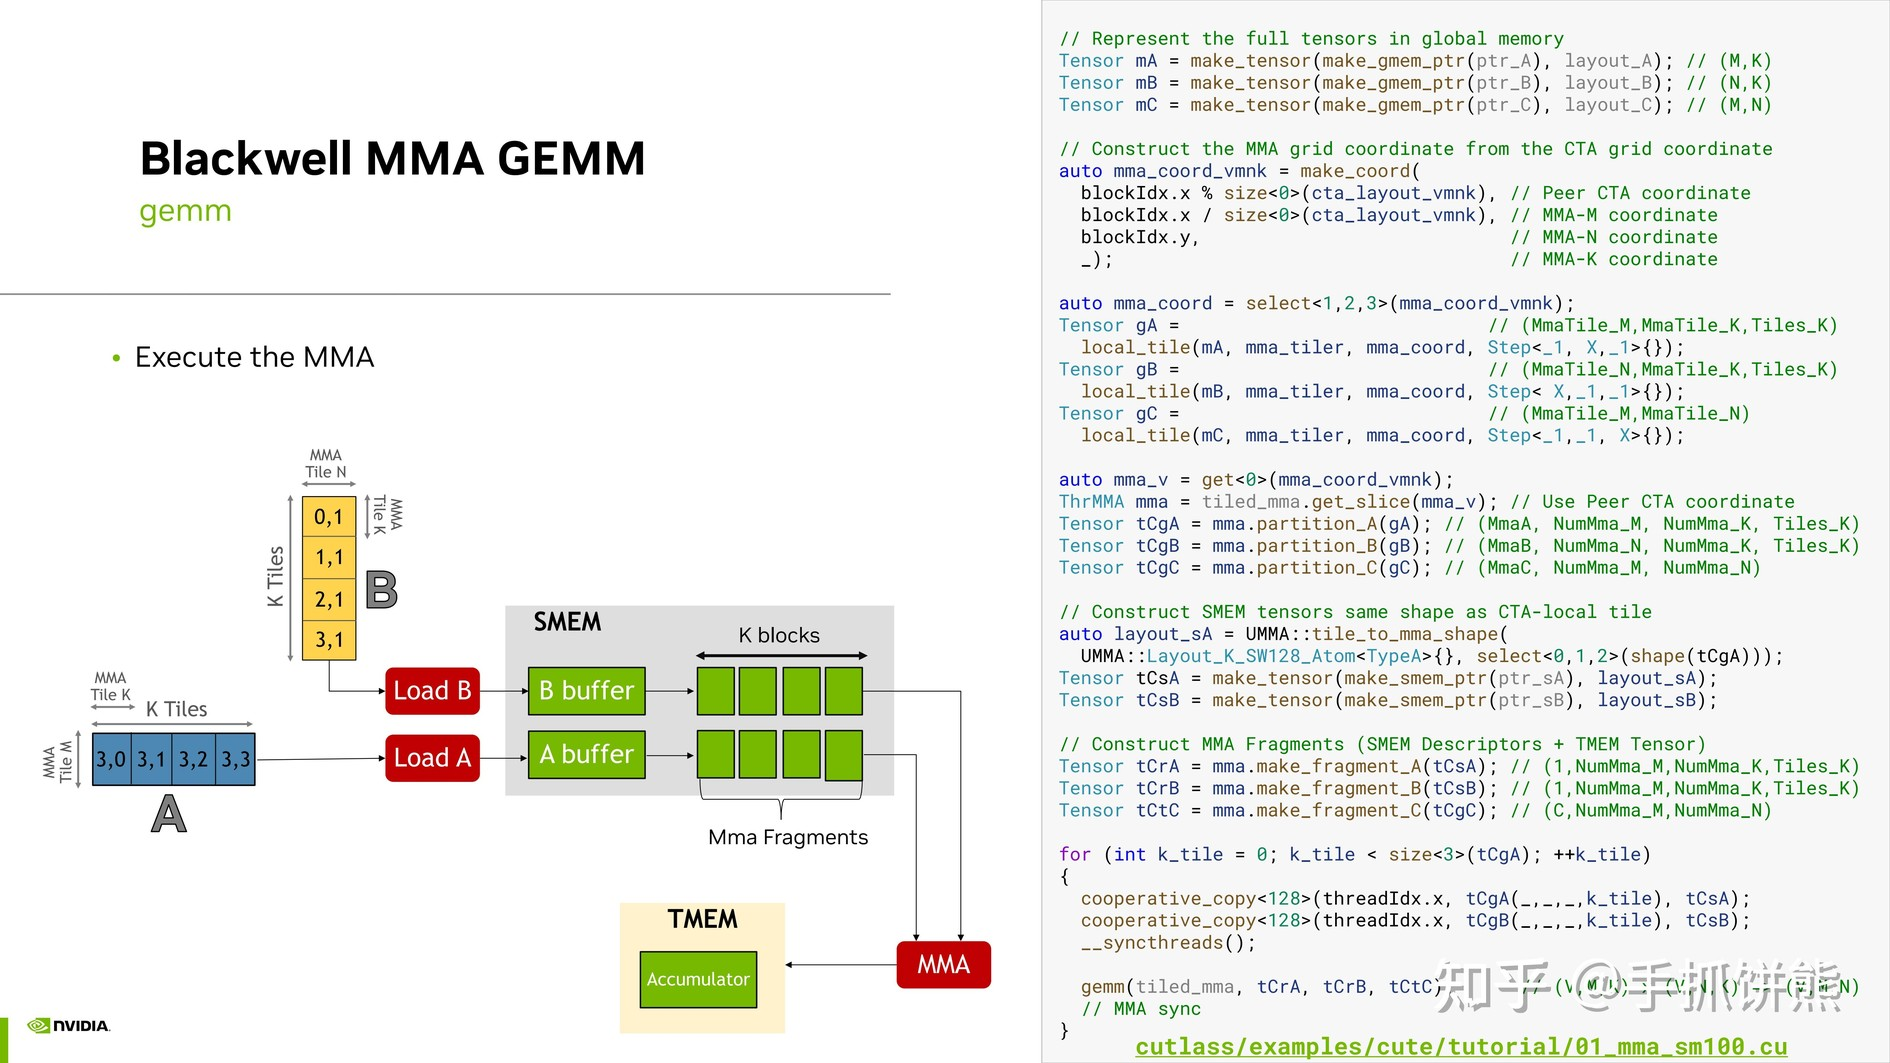
\includegraphics[width=0.9\textwidth]{figures/zhaoshangchun-01-tensor-core-programming/fig-28.jpg}
\end{figure}

万事俱备，只需调用 \texttt{g\allowbreak{}e\allowbreak{}m\allowbreak{}m\allowbreak{}(\allowbreak{}t\allowbreak{}i\allowbreak{}l\allowbreak{}e\allowbreak{}d\allowbreak{}\_\allowbreak{}m\allowbreak{}m\allowbreak{}a\allowbreak{},\allowbreak{} \allowbreak{}t\allowbreak{}C\allowbreak{}r\allowbreak{}A\allowbreak{},\allowbreak{} \allowbreak{}t\allowbreak{}C\allowbreak{}r\allowbreak{}B\allowbreak{},\allowbreak{} \allowbreak{}t\allowbreak{}C\allowbreak{}t\allowbreak{}C\allowbreak{})} 即可。这个函数会自动在 k-tile 循环的每次迭代中，下发 \texttt{tcgen05.\allowbreak{}mma} 指令，使用 \texttt{t\allowbreak{}Cr\allowbreak{}A} 和 \texttt{t\allowbreak{}Cr\allowbreak{}B}（SMEM 描述符）作为输入，将结果累加到 \texttt{t\allowbreak{}Ct\allowbreak{}C}（TMEM 累加器）中。这个完整的例子展示了 Cu\allowbreak{}Te 如何通过一系列富有表现力的、可组合的抽象，将一个复杂的 GEMM 计算任务分解为清晰的逻辑步骤。

\subsection{\textbf{异步数据加载与跨 SM 协作}}

本页开始将引入更高级的 Cu\allowbreak{}Te 特性，包括使用 TMA 实现数据加载与计算的流水线，以及如何编程跨 SM 的 MMA 和 TMA 操作，以充分挖掘 Blackwell 的硬件潜力。

\textbf{第 29 页：章节议程过渡}

\begin{figure}[H]\centering
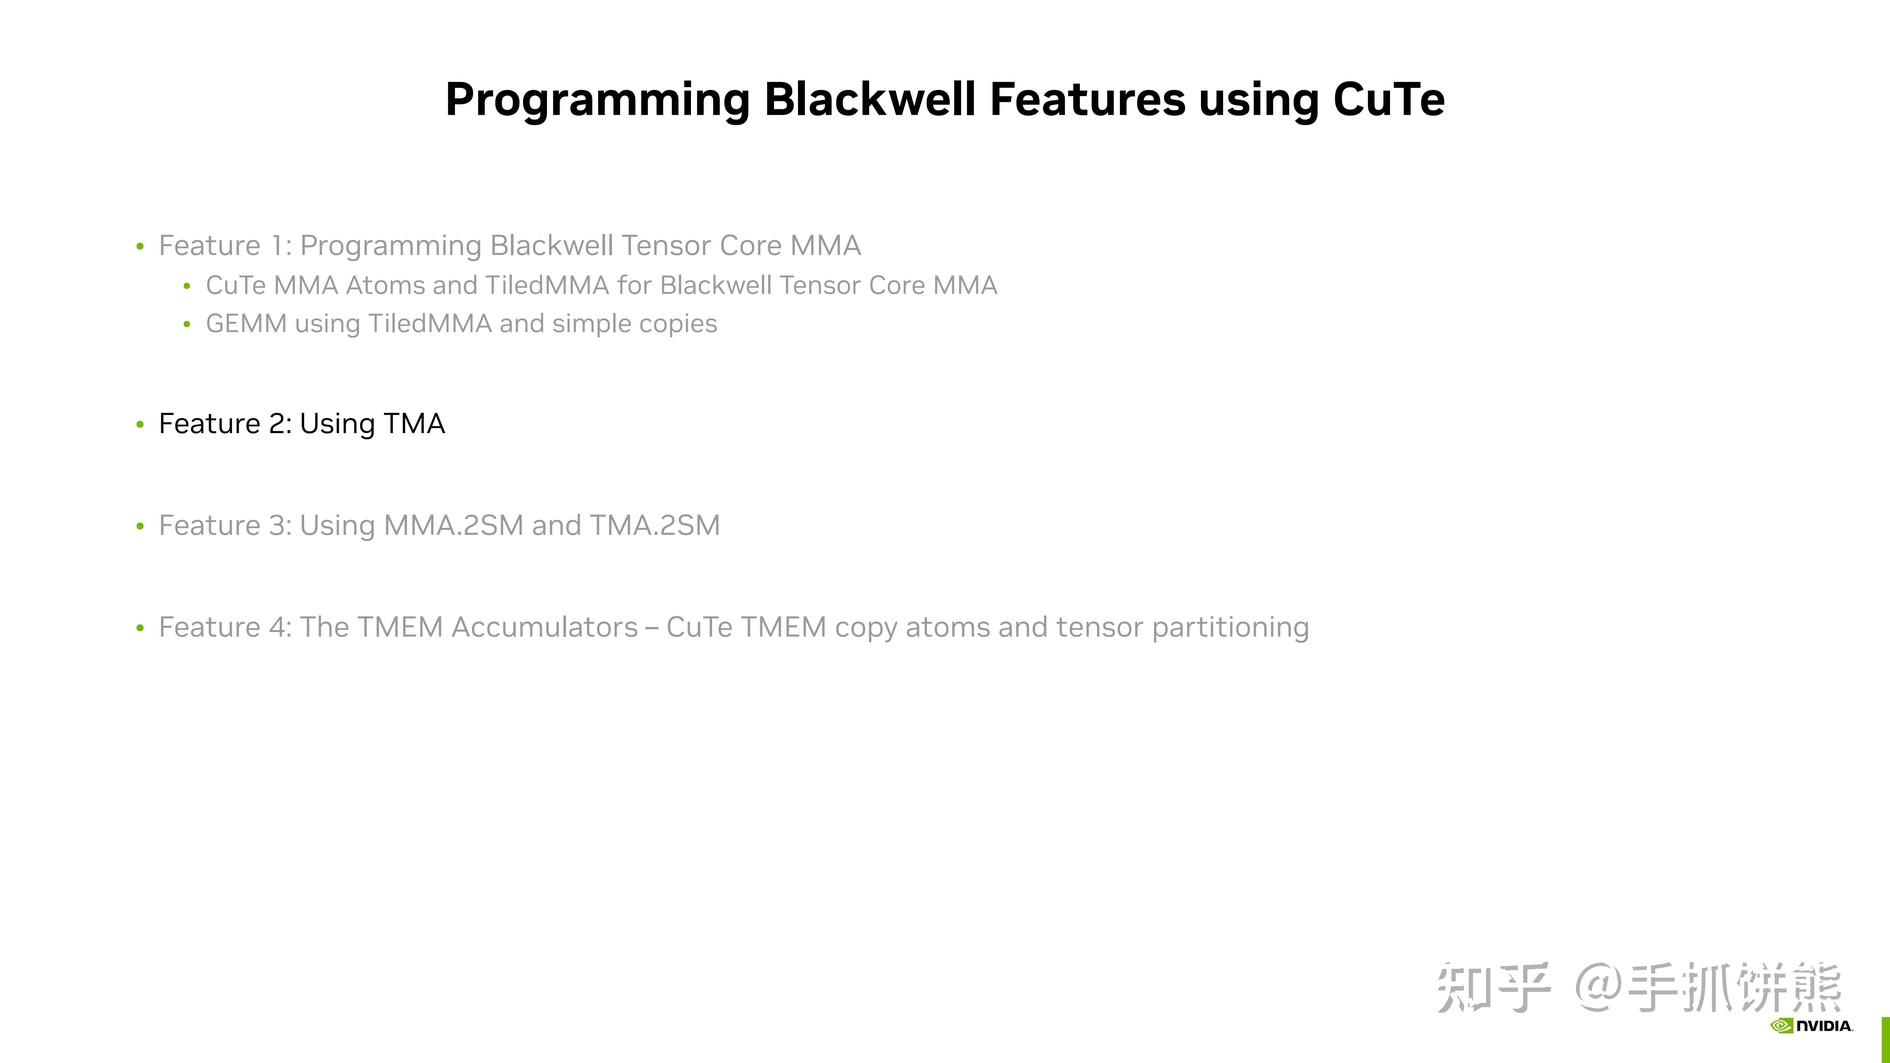
\includegraphics[width=0.9\textwidth]{figures/zhaoshangchun-01-tensor-core-programming/fig-29.jpg}
\end{figure}

本页开始进入异步数据加载部分。前面的 \texttt{cooperative\_\allowbreak{}copy} 是同步操作，会阻塞计算。而 TMA (Tensor Memory Access) 作为 Blackwell 的硬件加速器，允许我们在计算进行的同时，在后台异步地从全局内存预取下一个数据块，从而隐藏访存延迟。

掌握 TMA 是实现高性能核函数的关键一步。它要求我们以流水线（pipeline）的思维来组织代码，将数据流和计算流解耦。接下来，我们将看到 Cu\allowbreak{}Te 是如何帮助我们轻松实现这一点的。

\textbf{第 30 页：TMA Atom}

\begin{figure}[H]\centering
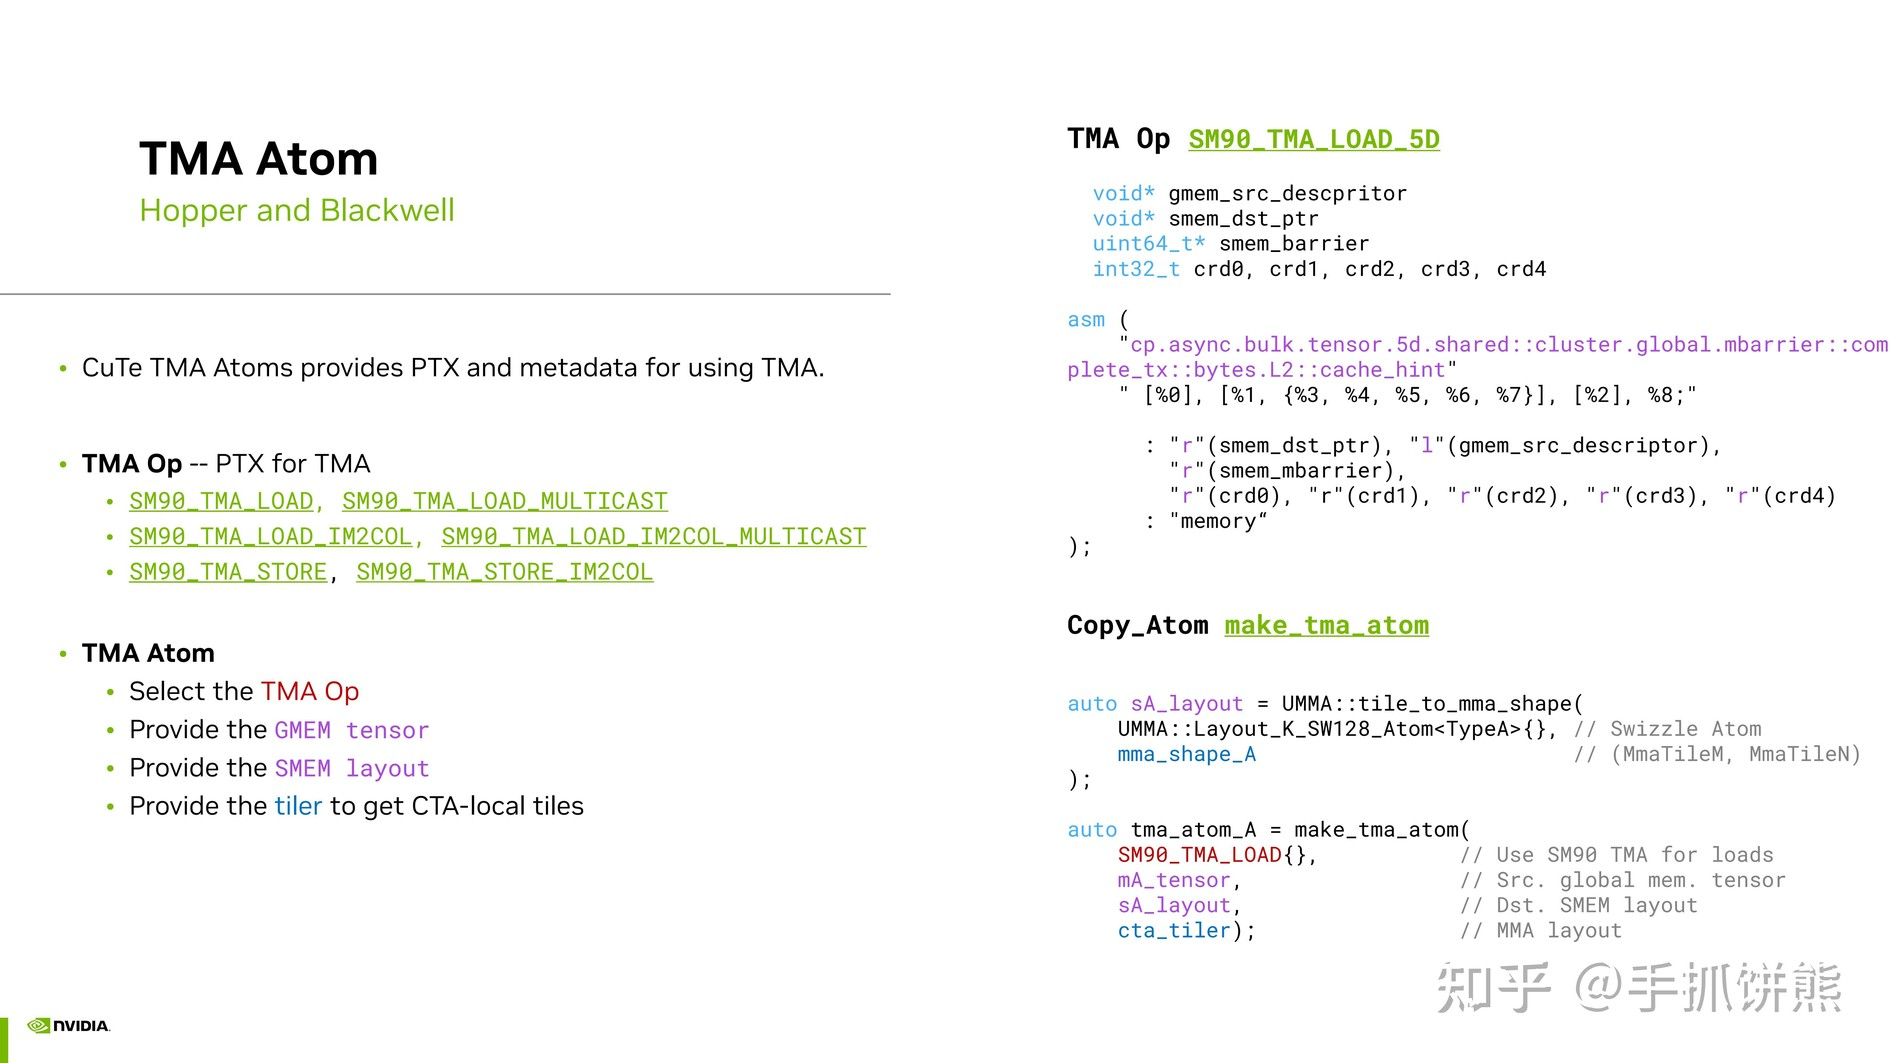
\includegraphics[width=0.9\textwidth]{figures/zhaoshangchun-01-tensor-core-programming/fig-30.jpg}
\end{figure}

与 \texttt{MMA Atom} 类似，\texttt{TMA Atom} 是对硬件 \texttt{cp.\allowbreak{}async.\allowbreak{}bulk.\allowbreak{}tensor} 系列指令的封装。它包含了一个 \texttt{TMA Op}（PTX 汇编封装）和一系列用于描述拷贝操作的元数据，如源和目标的内存空间、数据布局等。\texttt{make\_\allowbreak{}tma\_\allowbreak{}atom} 工厂函数将一个 GMEM 张量、一个 SMEM 布局和一个 tiler 绑定在一起，创建一个 \texttt{Copy\_\allowbreak{}Atom}。

这个 \texttt{Copy\_\allowbreak{}Atom} 不仅仅是一个简单的函数，它是一个包含了完整“拷贝知识”的对象。它知道如何计算地址，如何处理边界条件，以及如何与硬件的 TMA 单元交互。这种高度的封装使得上层代码可以以一种声明式的方式来描述数据搬运任务，而无需关心底层的实现细节。

\textbf{第 31-33 页：在 GEMM 中使用 TMA}

\begin{figure}[H]\centering
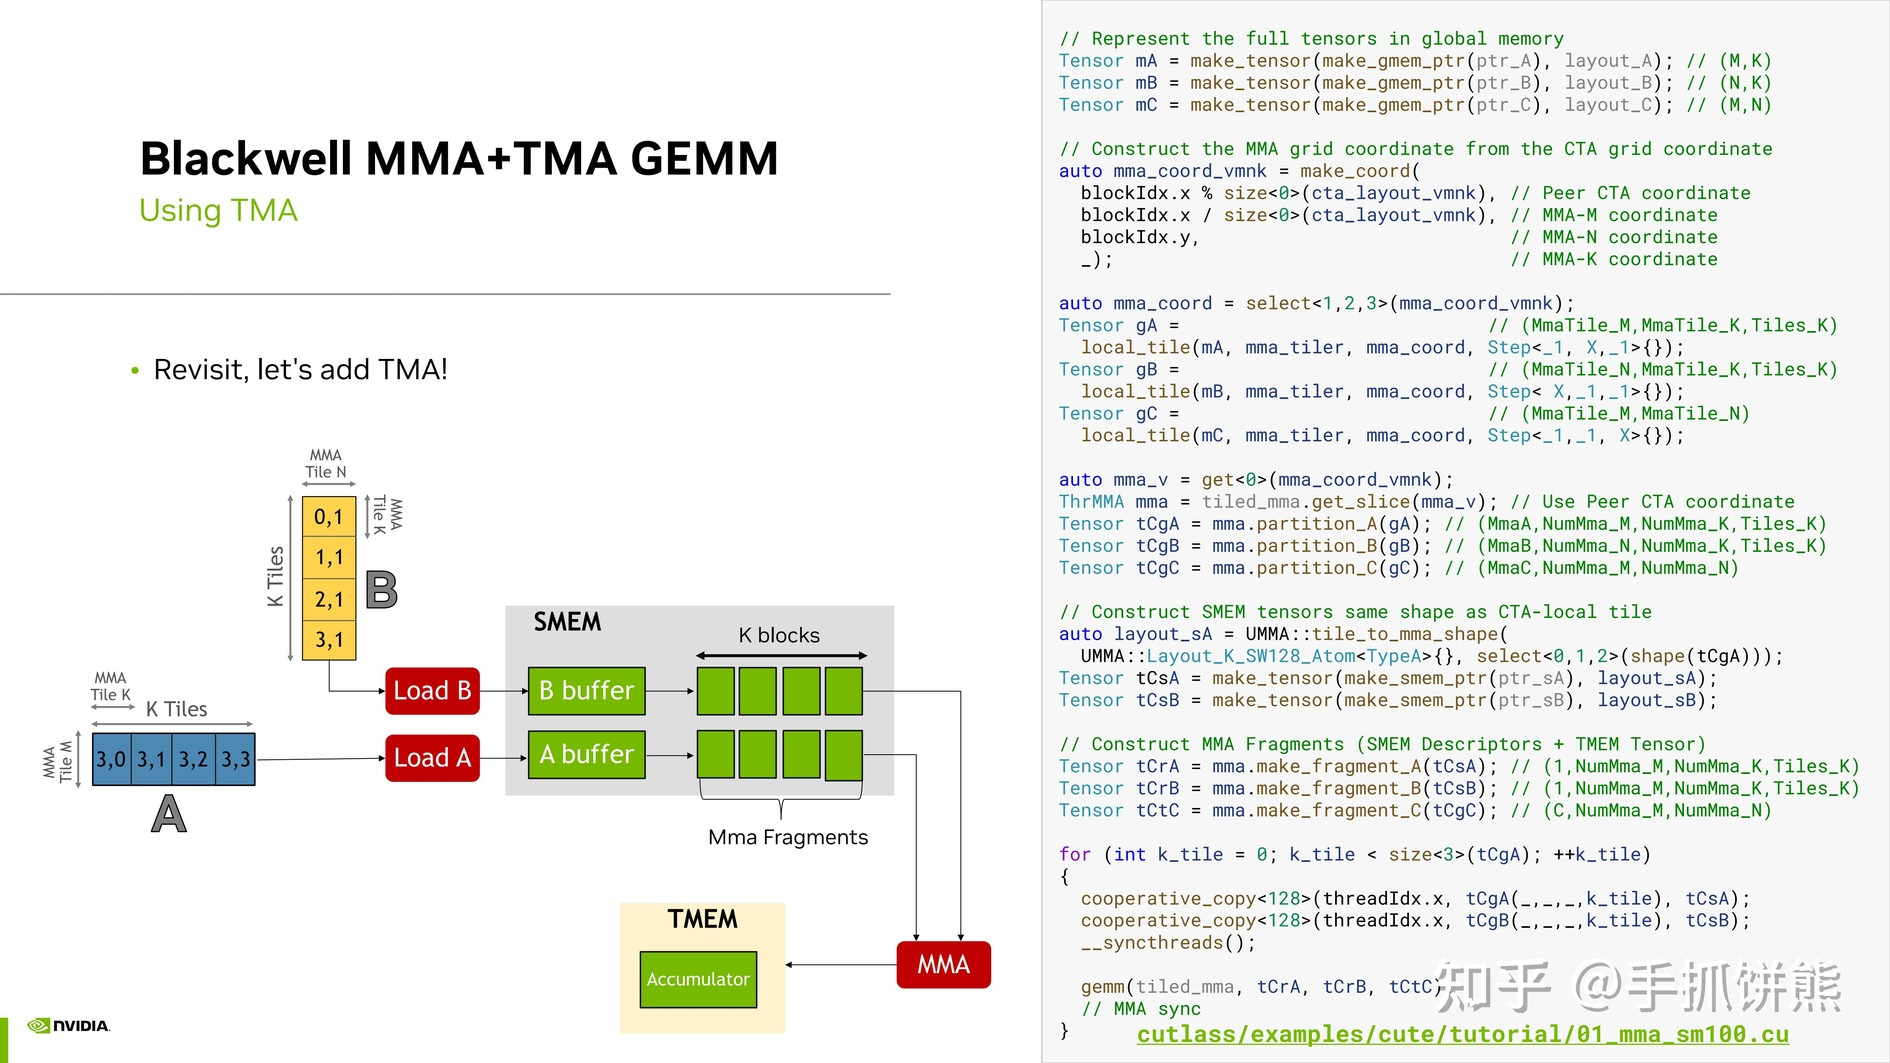
\includegraphics[width=0.9\textwidth]{figures/zhaoshangchun-01-tensor-core-programming/fig-31.jpg}
\end{figure}

\begin{figure}[H]\centering
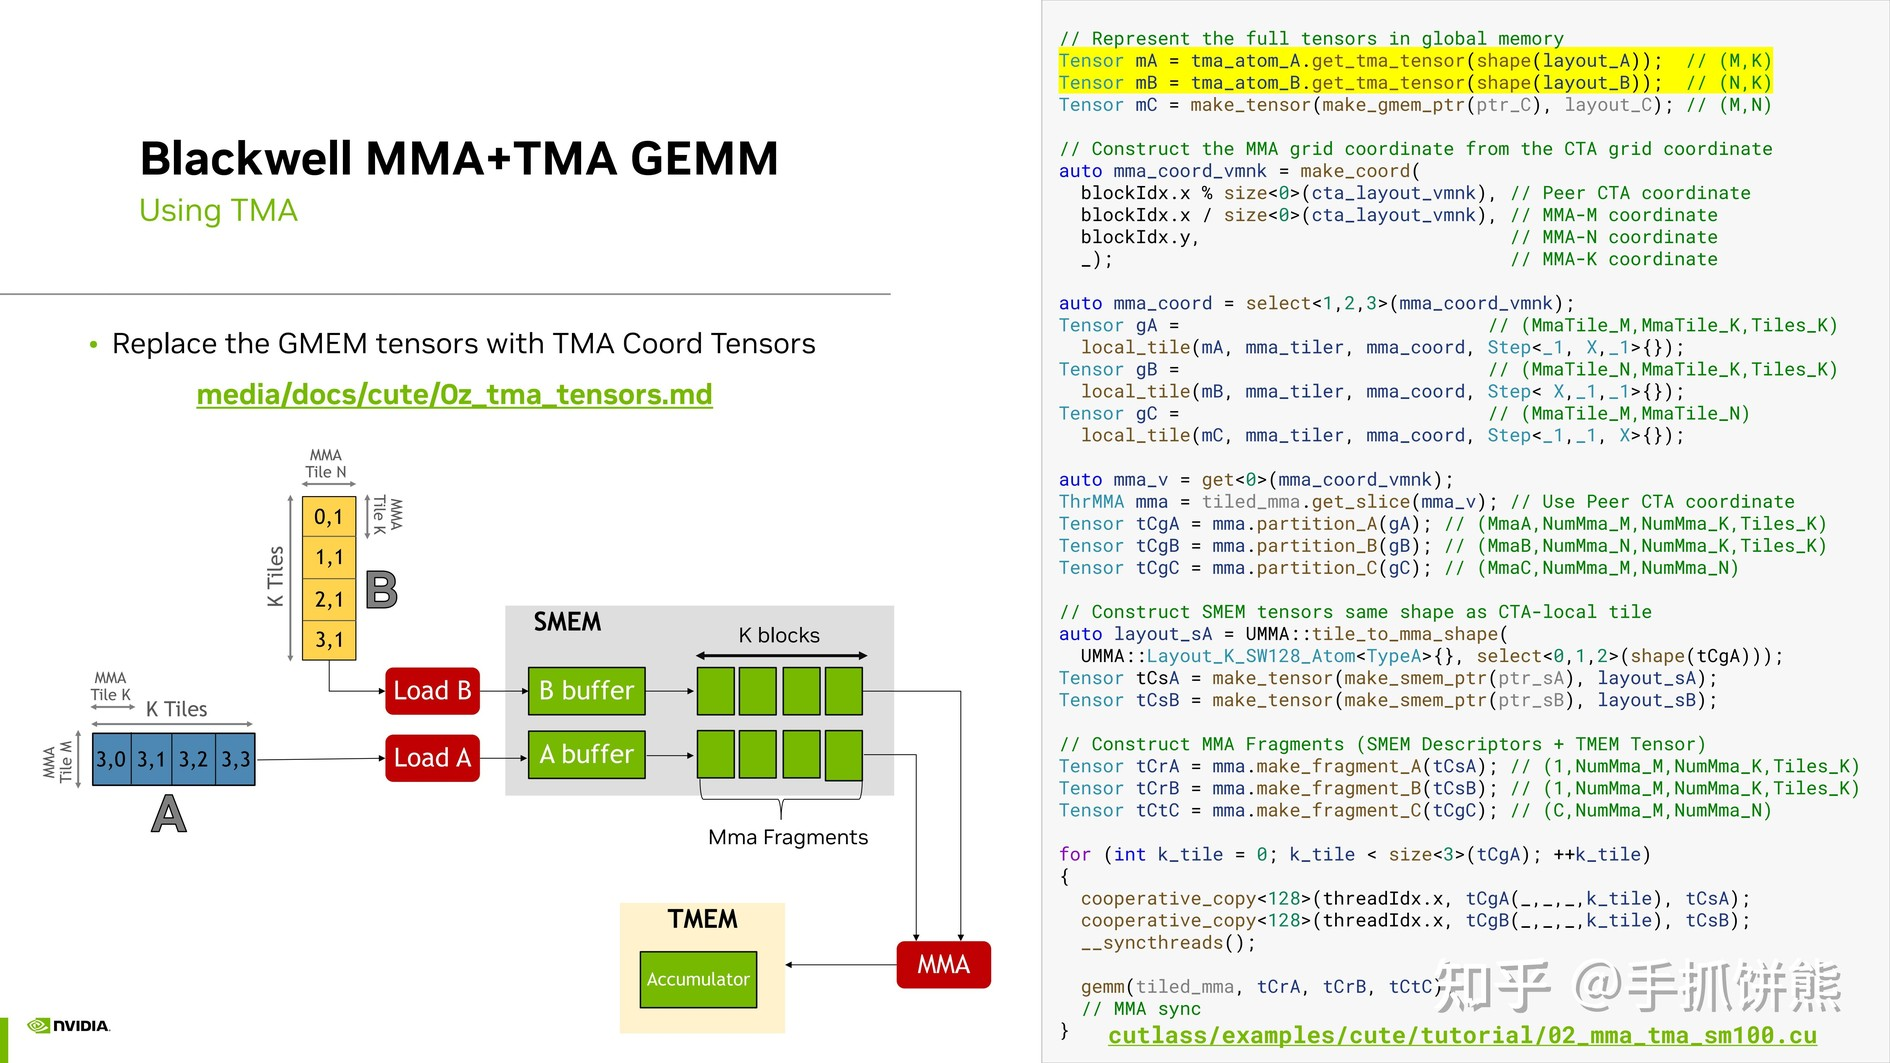
\includegraphics[width=0.9\textwidth]{figures/zhaoshangchun-01-tensor-core-programming/fig-32.jpg}
\end{figure}

\begin{figure}[H]\centering
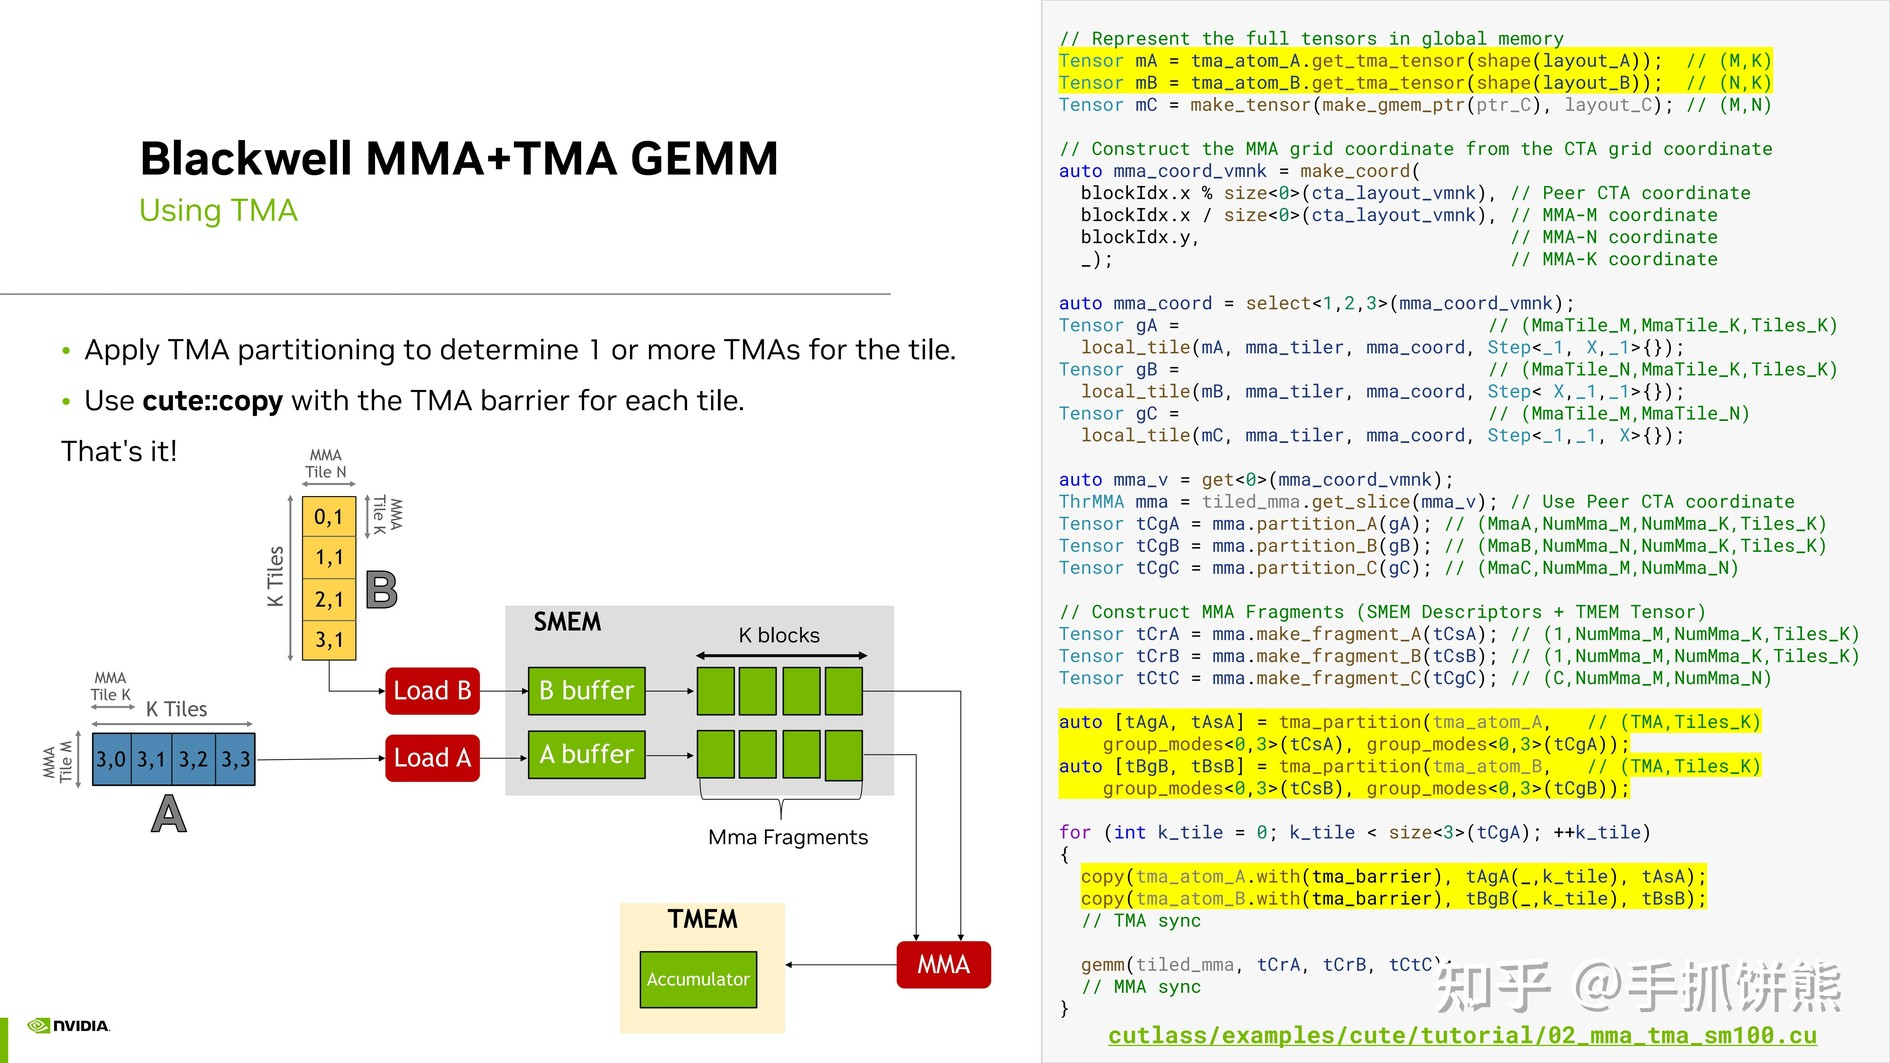
\includegraphics[width=0.9\textwidth]{figures/zhaoshangchun-01-tensor-core-programming/fig-33.jpg}
\end{figure}

将 \textbf{\texttt{cooperative\_\allowbreak{}copy} 替换为 TMA} 的过程非常直观。首先（第 32 页），将原始的 GMEM 张量替换为由 \texttt{tma\_\allowbreak{}atom} 生成的 TMA 坐标张量，其指针实际上是 TMA 描述符。然后（第 33 页），使用 \texttt{tma\_\allowbreak{}partition} 函数将整个拷贝任务划分为一系列小的 TMA 操作。最后（第 33 页），在主循环中，用 \texttt{c\allowbreak{}o\allowbreak{}p\allowbreak{}y\allowbreak{}(\allowbreak{}t\allowbreak{}m\allowbreak{}a\allowbreak{}\_\allowbreak{}a\allowbreak{}t\allowbreak{}o\allowbreak{}m\allowbreak{}\_\allowbreak{}A\allowbreak{}.\allowbreak{}w\allowbreak{}i\allowbreak{}t\allowbreak{}h\allowbreak{}(\allowbreak{}t\allowbreak{}m\allowbreak{}a\allowbreak{}\_\allowbreak{}b\allowbreak{}a\allowbreak{}r\allowbreak{}r\allowbreak{}i\allowbreak{}e\allowbreak{}r\allowbreak{})\allowbreak{},\allowbreak{} \allowbreak{}.\allowbreak{}.\allowbreak{}.\allowbreak{})} 来发起异步拷贝，并使用 \texttt{tma\_\allowbreak{}barrier} 对象进行同步。

TMA 的引入使得\textbf{数据加载（GMEM->SMEM）和计算（MMA）可以深度重叠（pipeline）}，从而隐藏访存延迟。这是现代 GPU 高性能计算的基石。Cu\allowbreak{}Te 将复杂的 TMA 描述符创建、地址计算和同步管理都封装在了 \texttt{TMA Atom} 和 \texttt{copy} 函数中，极大地简化了异步编程的复杂性，让开发者可以更专注于算法逻辑本身。

\subsection{MMA.2SM and TMA.2SM 及示例}

\textbf{第 34 页：章节议程}

\begin{figure}[H]\centering
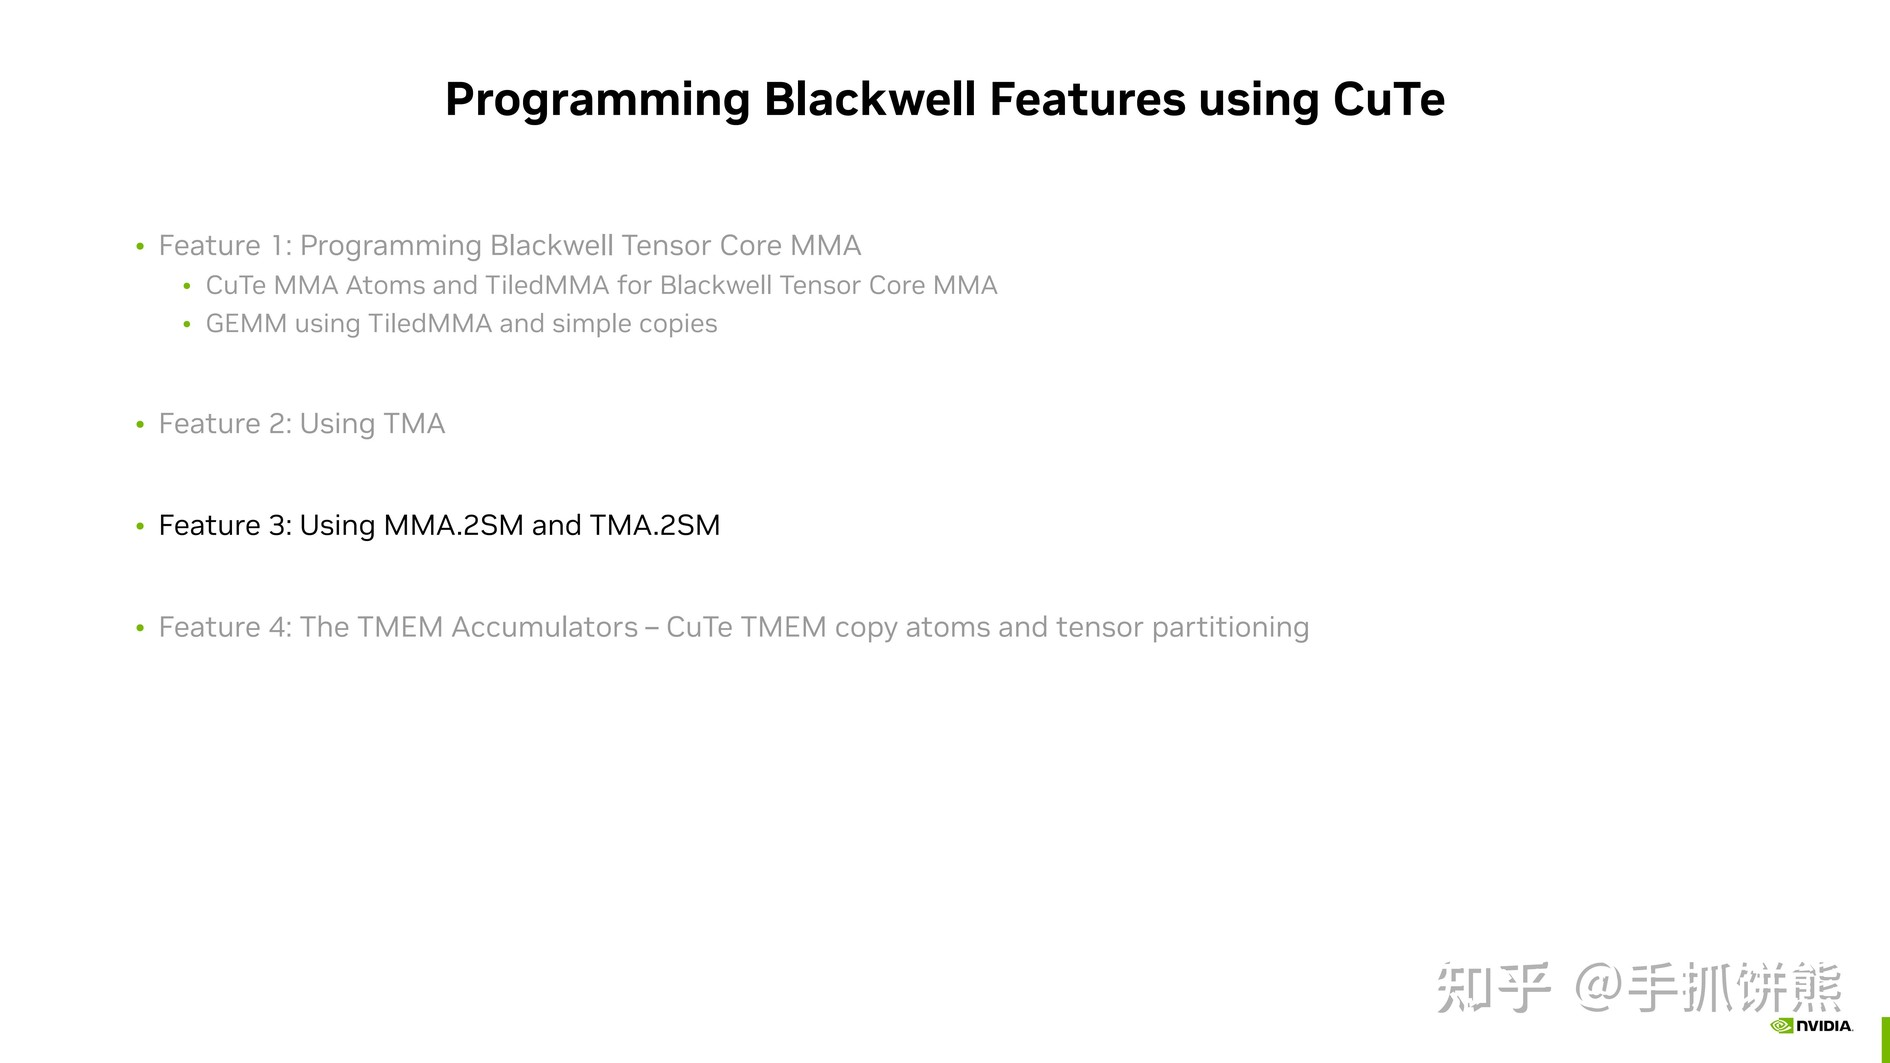
\includegraphics[width=0.9\textwidth]{figures/zhaoshangchun-01-tensor-core-programming/fig-34.jpg}
\end{figure}

这页开始Feature 3: Using MMA.2\allowbreak{}SM and TMA.2\allowbreak{}SM，从本页开始将要接触 Blackwell 架构的跨 SM 协作。前面的示例都是在单个 SM 内完成的，而 Blackwell 允许成对的 CTA 跨越两个 SM 进行协作，从而将计算和访存能力直接翻倍。

这不仅仅是性能的提升，更是编程模型的范式转变。开发者需要开始思考如何在 CTA-pair 的粒度上进行数据划分、任务分配和同步。幸运的是，Cu\allowbreak{}Te 再次提供了强大的抽象。

\textbf{第 35 页：Cu\allowbreak{}Te MMA Atoms}

\begin{figure}[H]\centering
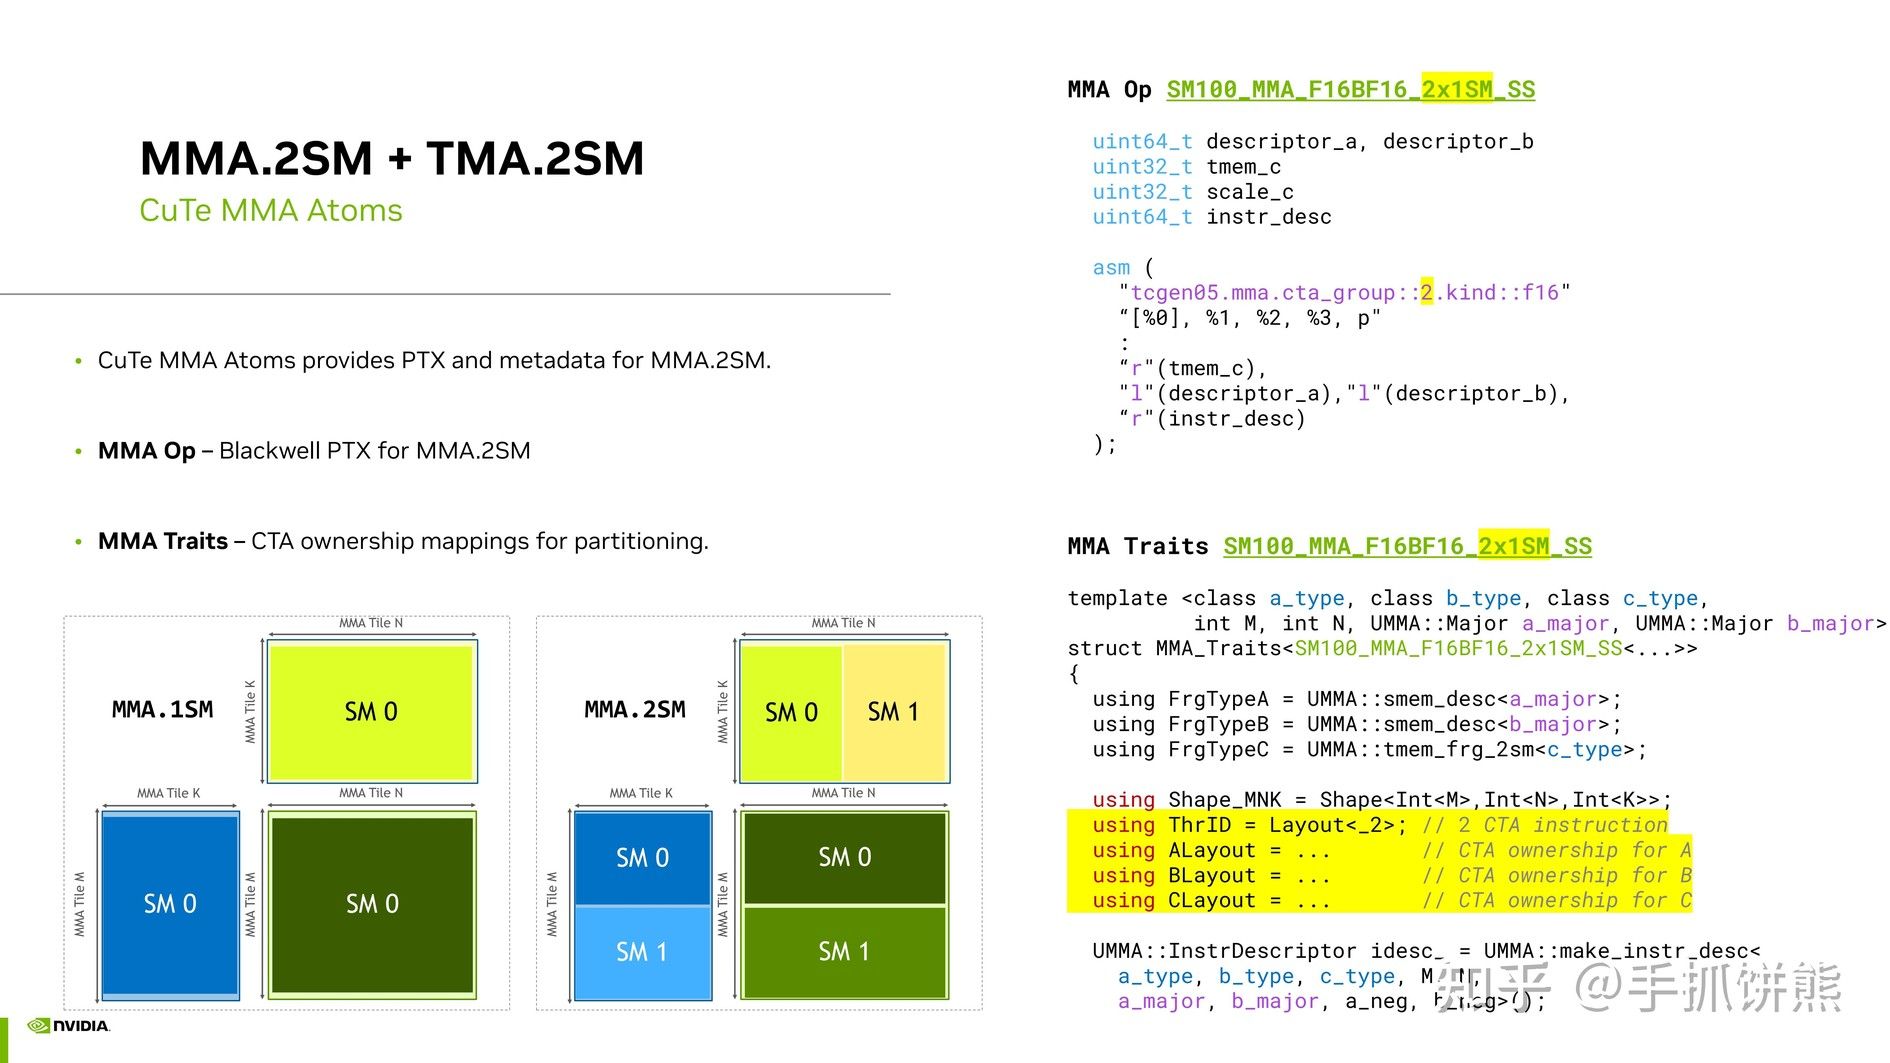
\includegraphics[width=0.9\textwidth]{figures/zhaoshangchun-01-tensor-core-programming/fig-35.jpg}
\end{figure}

这一页深入剖析了 Cu\allowbreak{}Te 如何通过 \texttt{MMA Atoms} 来抽象和使用 Blackwell 的 \texttt{MMA.\allowbreak{}2\allowbreak{}SM} 特性，即单个 MMA 操作横跨两个 SM 进行。这是 Blackwell 架构实现更高计算密度和效率的关键。

图示清晰地对比了 \texttt{MMA.\allowbreak{}1\allowbreak{}SM} 和 \texttt{MMA.\allowbreak{}2\allowbreak{}SM} 的区别。在 \texttt{MMA.\allowbreak{}1\allowbreak{}SM}（Hopper 及之前）模式下，一个 MMA tile 的计算完全由单个 SM 内的资源完成。而在 \texttt{MMA.\allowbreak{}2\allowbreak{}SM} 模式下，\textbf{一个逻辑上的 MMA tile 被物理地拆分到两个 SM 上}。如图所示，矩阵 A 的 M-K tile 和矩阵 B 的 K-N tile 的一部分位于 SM0，另一部分位于 SM1。这意味着两个 SM 上的 CTA 需要协同工作，共享输入数据并共同完成一次矩阵乘法。这种模式的\textbf{核心优势在于能够处理更大规模的 MMA tile}，从而摊薄控制开销、提高计算访存比，并更好地利用每个 SM 的计算资源。

为了在软件层面支持这种硬件行为，Cu\allowbreak{}Te 提供了 \texttt{MMA\_\allowbreak{}Traits} 和 \texttt{MMA Op} 两个核心抽象。\texttt{MMA Op} 直接对应底层的 PTX 指令，例如 \texttt{t\allowbreak{}c\allowbreak{}g\allowbreak{}e\allowbreak{}n\allowbreak{}0\allowbreak{}5\allowbreak{}.\allowbreak{}m\allowbreak{}m\allowbreak{}a\allowbreak{}.\allowbreak{}c\allowbreak{}t\allowbreak{}a\allowbreak{}\_\allowbreak{}g\allowbreak{}r\allowbreak{}o\allowbreak{}u\allowbreak{}p\allowbreak{}:\allowbreak{}:\allowbreak{}2\allowbreak{}.\allowbreak{}k\allowbreak{}i\allowbreak{}n\allowbreak{}d\allowbreak{}:\allowbreak{}:\allowbreak{}f\allowbreak{}1\allowbreak{}6}。这里的 \texttt{cta\_\allowbreak{}group::\allowbreak{}2} 明确指示了这是一个需要 \textbf{2 个 CTA 协作}完成的 MMA 操作。

\texttt{MMA\_\allowbreak{}Traits} 则是一个元编程工具，它定义了 \texttt{MMA.\allowbreak{}2\allowbreak{}SM} 操作所需的\textbf{元数据和布局信息}。\texttt{F\allowbreak{}r\allowbreak{}g\allowbreak{}T\allowbreak{}y\allowbreak{}p\allowbreak{}e\allowbreak{}C\allowbreak{} \allowbreak{}=\allowbreak{} \allowbreak{}U\allowbreak{}M\allowbreak{}M\allowbreak{}A\allowbreak{}:\allowbreak{}:\allowbreak{}t\allowbreak{}m\allowbreak{}e\allowbreak{}m\allowbreak{}\_\allowbreak{}f\allowbreak{}r\allowbreak{}g\allowbreak{}\_\allowbreak{}2\allowbreak{}s\allowbreak{}m\allowbreak{}<\allowbreak{}c\allowbreak{}\_\allowbreak{}t\allowbreak{}y\allowbreak{}p\allowbreak{}e\allowbreak{}>} 表明累加结果 C 的分片（fragment）将存储在跨两个 SM 的 TMEM 中。\texttt{Thr\allowbreak{}ID = Layout<\_\allowbreak{}2>} 则再次确认了这是一个 2-CTA 协作的指令。\texttt{ALayout}, \texttt{BLayout}, \texttt{CLayout} 定义了 A、B、C 张量在 CTA 组内的\textbf{数据归属（ownership）}，即哪个 CTA 负责提供和计算哪部分数据。\texttt{UMMA::\allowbreak{}make\_\allowbreak{}instr\_\allowbreak{}desc} 则根据模板参数生成 MMA 指令所需的描述符，将高层 C++ 类型信息编译成硬件可识别的格式。

\texttt{MMA.\allowbreak{}2\allowbreak{}SM} 的引入对性能有巨大影响，但编程复杂度也相应增加。开发者需要精确管理两个 CTA 之间的数据共享、同步以及计算任务的划分。Cu\allowbreak{}Te 的价值在于\textbf{将这些复杂的硬件细节封装在高层、可组合的 C++ 模板中}。通过使用 \texttt{MMA\_\allowbreak{}Traits}，开发者可以声明式地定义一个 \texttt{2x1\allowbreak{}SM} 的 MMA 策略，而 Cu\allowbreak{}Te 的编译期机制会自动处理数据分区、线程映射和指令生成。这使得开发者能够以接近于单 SM 编程的思维模式，来利用跨 SM 计算的强大能力，从而在不牺牲可维护性的前提下，充分压榨 Blackwell 硬件的性能潜力。\texttt{tmem\_\allowbreak{}frg\_\allowbreak{}2sm} 的使用也暗示了累加器现在可以安放在 TMEM 中，这大大缓解了寄存器压力，为更复杂的算子融合提供了宝贵的寄存器资源。

\textbf{第 36 页：Cu\allowbreak{}Te Copy Atoms}

\begin{figure}[H]\centering
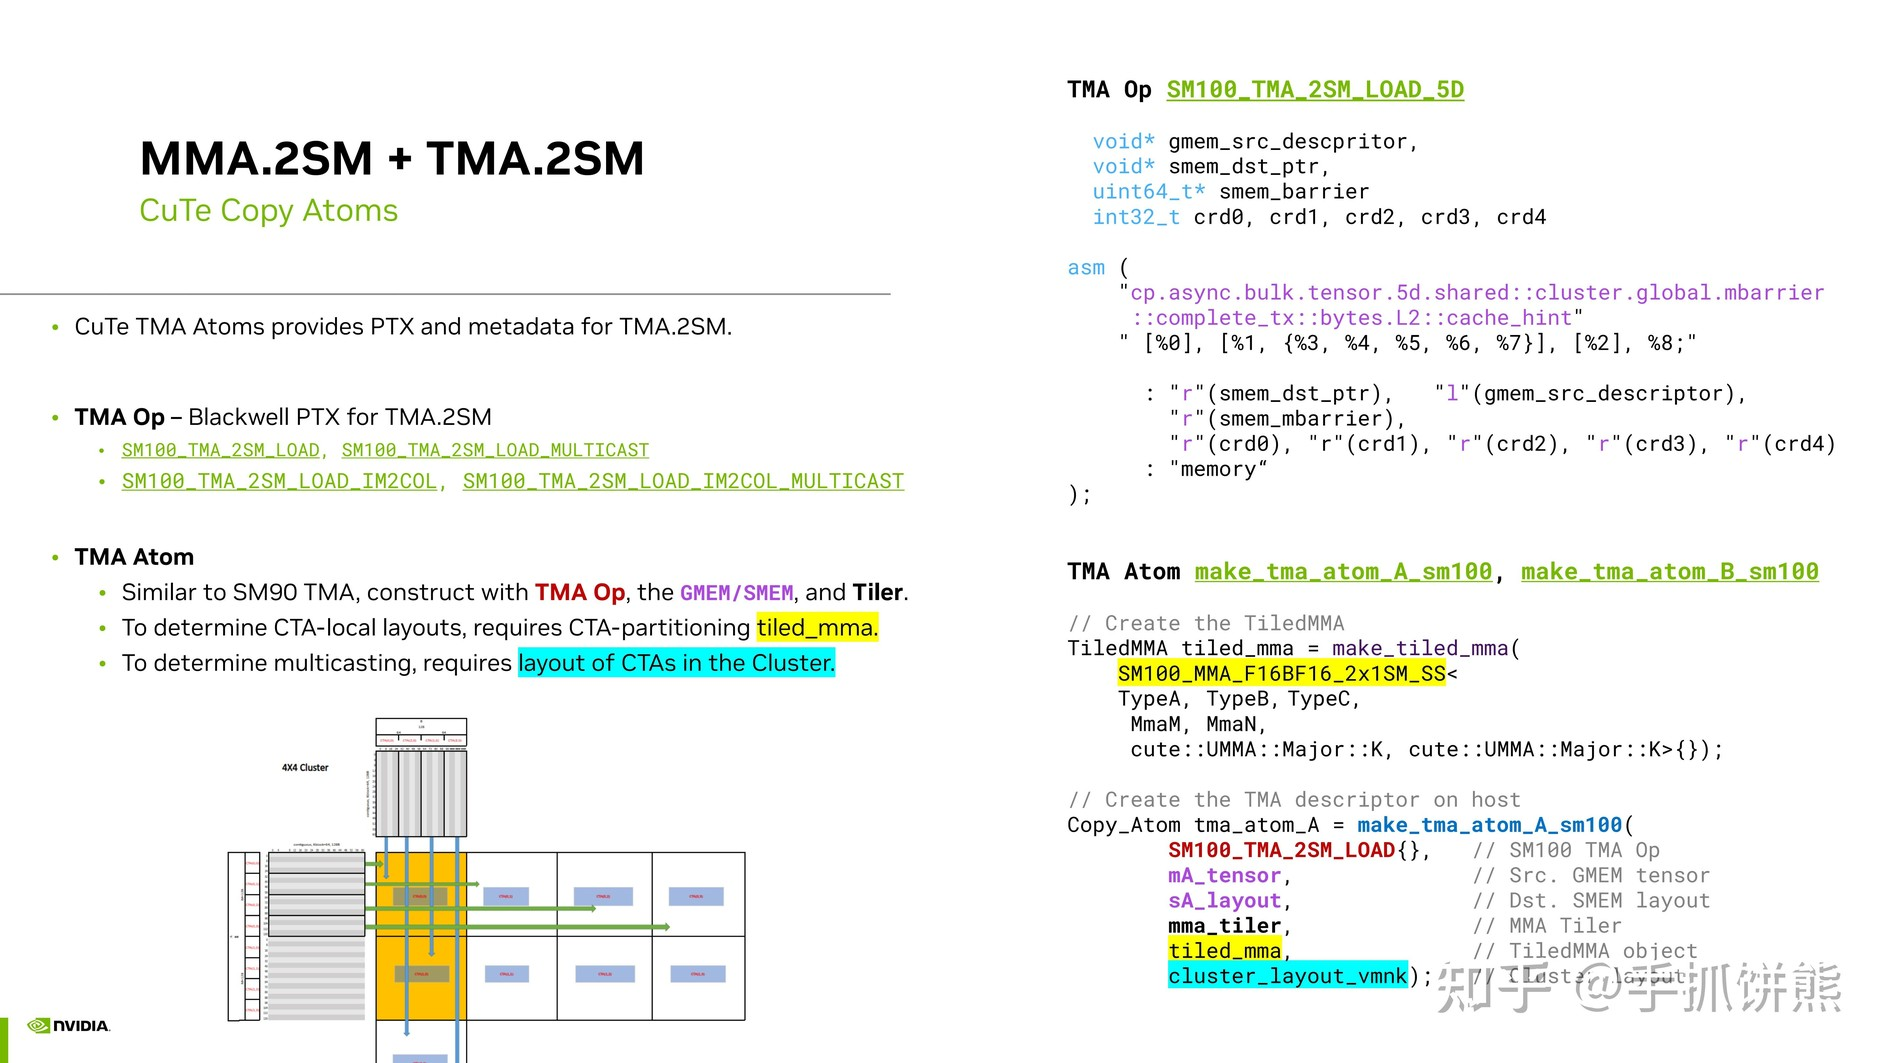
\includegraphics[width=0.9\textwidth]{figures/zhaoshangchun-01-tensor-core-programming/fig-36.jpg}
\end{figure}

继 \texttt{MMA.\allowbreak{}2\allowbreak{}SM} 之后，这一页展示了 Cu\allowbreak{}Te 如何通过 \texttt{Copy Atoms} 来编程 \texttt{TMA.\allowbreak{}2\allowbreak{}SM}，即\textbf{横跨两个 SM 的 Tensor Memory Accelerator 数据加载}。这与 \texttt{MMA.\allowbreak{}2\allowbreak{}SM} 相辅相成，共同构成了 Blackwell 大规模并行计算的基础。

\texttt{c\allowbreak{}p\allowbreak{}.\allowbreak{}a\allowbreak{}s\allowbreak{}y\allowbreak{}n\allowbreak{}c\allowbreak{}.\allowbreak{}b\allowbreak{}u\allowbreak{}l\allowbreak{}k\allowbreak{}.\allowbreak{}t\allowbreak{}e\allowbreak{}n\allowbreak{}s\allowbreak{}o\allowbreak{}r\allowbreak{}.\allowbreak{}5\allowbreak{}d\allowbreak{}.\allowbreak{}s\allowbreak{}h\allowbreak{}a\allowbreak{}r\allowbreak{}e\allowbreak{}d\allowbreak{}:\allowbreak{}:\allowbreak{}c\allowbreak{}l\allowbreak{}u\allowbreak{}s\allowbreak{}t\allowbreak{}e\allowbreak{}r\allowbreak{}.\allowbreak{}g\allowbreak{}l\allowbreak{}o\allowbreak{}b\allowbreak{}a\allowbreak{}l\allowbreak{}.\allowbreak{}m\allowbreak{}b\allowbreak{}a\allowbreak{}r\allowbreak{}r\allowbreak{}i\allowbreak{}e\allowbreak{}r} 这条新的 PTX 指令。我们来逐段解析这个指令的含义：

\begin{itemize}
\item \texttt{cp.\allowbreak{}async.\allowbreak{}bulk}：表示这是一次\textbf{异步、批量}的数据拷贝操作，CPU（这里指 SM 中的控制单元）发出指令后可以继续执行其他任务，无需等待拷贝完成。
\item \texttt{tensor.\allowbreak{}5d}：说明 TMA 现在支持高达 \textbf{5\allowbreak{}D 的张量描述符}，可以描述非常复杂的数据布局（如 \texttt{NHWCD} 格式的卷积数据），而无需在软件层面进行繁琐的地址计算。
\item \texttt{shared::\allowbreak{}cluster}：目标地址是 SMEM，并且这个拷贝是在一个 \textbf{CTA Cluster} 的上下文中执行的。这意味着加载的数据可以被 Cluster 内的多个 CTA 共享（multicast），极大地减少了从全局内存（GMEM）读取的次数。
\item \texttt{global.\allowbreak{}mbarrier}：使用 \texttt{mbarrier} 对象进行同步。\texttt{mbarrier} 是 Hopper 引入的、在 SMEM 中分配的屏障对象，用于管理异步操作的依赖关系。CPU 可以通过 \texttt{mbarrier} 来等待 TMA 操作完成。
\end{itemize}

Cu\allowbreak{}Te 将这些复杂的 PTX 指令封装在 \texttt{TMA Atom} 中。\texttt{make\_\allowbreak{}tma\_\allowbreak{}atom\_\allowbreak{}A\_\allowbreak{}sm100} 工厂函数展示了如何创建一个 TMA 加载操作。它需要几个关键输入：

\begin{enumerate}
\item \texttt{SM100\_\allowbreak{}TMA\_\allowbreak{}2\allowbreak{}SM\_\allowbreak{}LOAD\{\}}：一个操作类型，指明使用 Blackwell 架构的 \texttt{TMA.\allowbreak{}2\allowbreak{}SM} 加载功能。CUTLASS 还提供了 \texttt{\_\allowbreak{}MULTICAST} 和 \texttt{\_\allowbreak{}IM2\allowbreak{}COL} 等变体，分别用于广播加载和卷积中的 \texttt{im2col} 操作。
\item \texttt{m\allowbreak{}A\_\allowbreak{}tensor}：源张量，位于 GMEM。
\item \texttt{s\allowbreak{}A\_\allowbreak{}layout}：目标张量在 SMEM 中的布局。
\item \texttt{mma\_\allowbreak{}tiler} 和 \texttt{tiled\_\allowbreak{}mma}：这两个对象描述了\textbf{计算（MMA）}是如何对问题进行切分的。TMA 需要知道计算侧的 tile 布局，才能以最优的方式从 GMEM 中抓取数据并放置到 SMEM 中，保证后续的 MMA 操作能高效读取。
\item \texttt{cluster\_\allowbreak{}layout\_\allowbreak{}vmnk}：CTA Cluster 的布局。TMA 需要这个信息来判断是否以及如何执行 \texttt{multicast}。
\end{enumerate}

开发者首先定义好 \texttt{Tiled\allowbreak{}MMA}（计算如何进行），然后将这个计算模式“告知”TMA Atom。TMA Atom 会根据计算的需求，自动生成最优的数据加载指令。特别是“To determine CTA-local layouts, requires CTA-partitioning tiled\_\allowbreak{}mma”这句话，点明了数据布局的决定权在于计算本身。这与传统的手写 CUDA 核中，开发者需要同时手动管理加载地址和计算逻辑相比，\textbf{极大地简化了高性能 GEMM 内核的开发}，降低了出错的可能性，并使得代码更容易适应不同的矩阵尺寸和硬件配置。

\textbf{第 37 页：Blackwell GEMM 示例代码解析 - 坐标、分片与流水线}

\begin{figure}[H]\centering
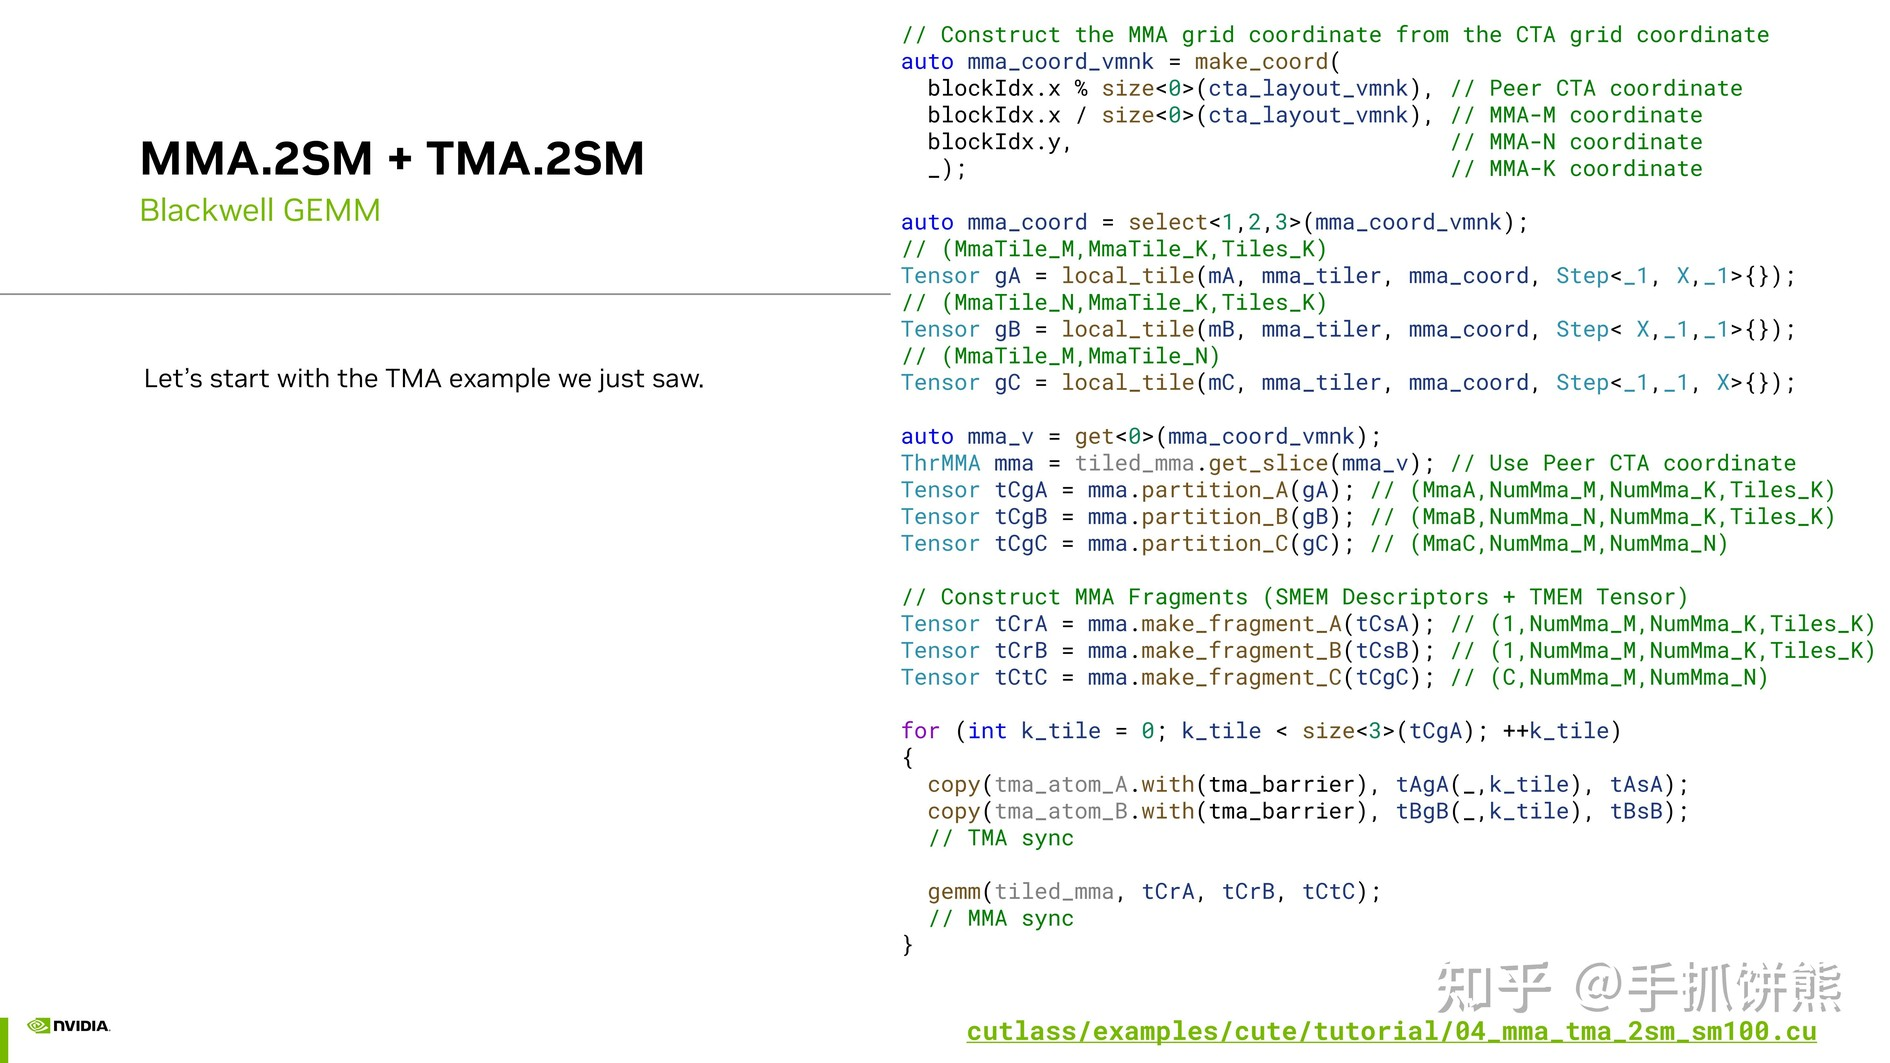
\includegraphics[width=0.9\textwidth]{figures/zhaoshangchun-01-tensor-core-programming/fig-37.jpg}
\end{figure}

这一页开始通过一个具体的代码示例 \texttt{04\_\allowbreak{}mma\_\allowbreak{}tma\_\allowbreak{}2sm\_\allowbreak{}sm100.\allowbreak{}cu}，展示如何将前面介绍的 \texttt{Tiled\allowbreak{}MMA} 和 \texttt{TMA Atom} 组合起来，实现一个完整的、利用 \texttt{MMA.\allowbreak{}2\allowbreak{}SM} 和 \texttt{TMA.\allowbreak{}2\allowbreak{}SM} 的 GEMM 内核。

代码的第一部分是\textbf{坐标计算和张量视图的构建}。\texttt{mma\_\allowbreak{}coord\_\allowbreak{}vmnk} 的计算是理解 \texttt{2\allowbreak{}SM} 模型的关键。\texttt{block\allowbreak{}Idx.\allowbreak{}x} 被用来计算两个维度的坐标：\texttt{Peer CTA coordinate} 和 \texttt{MMA-M coordinate}。

\begin{itemize}
\item \texttt{Peer CTA coordinate}（\texttt{get<0>(mma\_\allowbreak{}coord\_\allowbreak{}vmnk)}）：值为 0 或 1，用于标识当前 CTA 在一个 2-CTA 组中是“leader”（0）还是“follower”（1）。
\item \texttt{MMA-M coordinate}：表示当前 CTA 组在整个 GEMM 问题的 M 维度上负责哪一个 tile。这种设计意味着，\textbf{\texttt{block\allowbreak{}Idx.\allowbreak{}x} 的连续两个值（例如 0 和 1）会映射到同一个 M、N tile，但分属不同的 Peer CTA}。\texttt{m\allowbreak{}m\allowbreak{}a\allowbreak{}\_\allowbreak{}v\allowbreak{} \allowbreak{}=\allowbreak{} \allowbreak{}g\allowbreak{}e\allowbreak{}t\allowbreak{}<\allowbreak{}0\allowbreak{}>\allowbreak{}(\allowbreak{}m\allowbreak{}m\allowbreak{}a\allowbreak{}\_\allowbreak{}c\allowbreak{}o\allowbreak{}o\allowbreak{}r\allowbreak{}d\allowbreak{}\_\allowbreak{}v\allowbreak{}m\allowbreak{}n\allowbreak{}k\allowbreak{})} 抽取出这个 Peer ID，并在 \texttt{t\allowbreak{}i\allowbreak{}l\allowbreak{}e\allowbreak{}d\allowbreak{}\_\allowbreak{}m\allowbreak{}m\allowbreak{}a\allowbreak{}.\allowbreak{}g\allowbreak{}e\allowbreak{}t\allowbreak{}\_\allowbreak{}s\allowbreak{}l\allowbreak{}i\allowbreak{}c\allowbreak{}e\allowbreak{}(\allowbreak{}m\allowbreak{}m\allowbreak{}a\allowbreak{}\_\allowbreak{}v\allowbreak{})} 中使用，以此来获取当前 CTA 在这个 2-CTA 组中应该承担的角色和数据分片。
\end{itemize}

接下来，代码通过 \texttt{local\_\allowbreak{}tile} 和 \texttt{partition\_\allowbreak{}A/\allowbreak{}B/\allowbreak{}C} 函数，将全局张量（\texttt{m\allowbreak{}A}, \texttt{m\allowbreak{}B}, \texttt{m\allowbreak{}C}）层层剖分，最终得到每个线程所需处理的数据分片。

\begin{itemize}
\item \texttt{local\_\allowbreak{}tile}：根据 \texttt{mma\_\allowbreak{}coord} 从全局张量中切出当前 CTA 组负责的 tile。
\item \texttt{mma.\allowbreak{}partition\_\allowbreak{}A/\allowbreak{}B/\allowbreak{}C}：\texttt{Thr\allowbreak{}MMA} 对象（\texttt{tiled\_\allowbreak{}mma} 的一个 slice）的核心功能，它根据当前线程在 CTA 内的 ID 和 Peer CTA ID，将 CTA 组的 tile 进一步划分为每个线程负责的\textbf{物理数据块}。
\item \texttt{mma.\allowbreak{}make\_\allowbreak{}fragment\_\allowbreak{}A/\allowbreak{}B/\allowbreak{}C}：这一步是 Cu\allowbreak{}Te 抽象的精髓。它并不直接创建数据，而是创建\textbf{描述符（descriptor）}。\texttt{t\allowbreak{}Cr\allowbreak{}A} 和 \texttt{t\allowbreak{}Cr\allowbreak{}B} 是 SMEM 描述符，指向 SMEM 中的数据。\texttt{t\allowbreak{}Ct\allowbreak{}C} 则是 TMEM 张量，代表了累加结果在 TMEM 中的布局。
\end{itemize}

最后是主循环 \texttt{for (int k\_\allowbreak{}tile = .\allowbreak{}.\allowbreak{}.\allowbreak{})}，它完美地展示了\textbf{经典的 GEMM 流水线（pipeline）}。

\begin{itemize}
\item \texttt{c\allowbreak{}o\allowbreak{}p\allowbreak{}y\allowbreak{}(\allowbreak{}t\allowbreak{}m\allowbreak{}a\allowbreak{}\_\allowbreak{}a\allowbreak{}t\allowbreak{}o\allowbreak{}m\allowbreak{}\_\allowbreak{}A\allowbreak{}.\allowbreak{}w\allowbreak{}i\allowbreak{}t\allowbreak{}h\allowbreak{}(\allowbreak{}t\allowbreak{}m\allowbreak{}a\allowbreak{}\_\allowbreak{}b\allowbreak{}a\allowbreak{}r\allowbreak{}r\allowbreak{}i\allowbreak{}e\allowbreak{}r\allowbreak{})\allowbreak{},\allowbreak{} \allowbreak{}.\allowbreak{}.\allowbreak{}.\allowbreak{})}：发出异步 TMA 加载指令，将 GMEM 中的 A 矩阵的一个 K-tile 拷贝到 SMEM。\texttt{.\allowbreak{}with(tma\_\allowbreak{}barrier)} 将这个操作与一个 \texttt{mbarrier} 关联起来。
\item \texttt{/\allowbreak{}/\allowbreak{} TMA sync}：在这里，内核会等待 \texttt{mbarrier}，确保数据已经到达 SMEM。
\item \texttt{g\allowbreak{}e\allowbreak{}m\allowbreak{}m\allowbreak{}(\allowbreak{}t\allowbreak{}i\allowbreak{}l\allowbreak{}e\allowbreak{}d\allowbreak{}\_\allowbreak{}m\allowbreak{}m\allowbreak{}a\allowbreak{},\allowbreak{} \allowbreak{}t\allowbreak{}C\allowbreak{}r\allowbreak{}A\allowbreak{},\allowbreak{} \allowbreak{}t\allowbreak{}C\allowbreak{}r\allowbreak{}B\allowbreak{},\allowbreak{} \allowbreak{}t\allowbreak{}C\allowbreak{}t\allowbreak{}C\allowbreak{})}：在数据准备好后，调用 \texttt{gemm} 函数执行 MMA 计算。
\item \texttt{/\allowbreak{}/\allowbreak{} MMA sync}：等待 MMA 计算完成。通过双缓冲（或多缓冲）技术，数据加载（\texttt{copy}）和计算（\texttt{gemm}）可以高度重叠：当一个 K-tile 正在计算时，下一个 K-tile 已经在被异步加载。这就是高性能 GEMM 内核隐藏访存延迟的核心机制。
\end{itemize}

\textbf{第 38 页：Blackwell GEMM 示例代码解析 - 2\allowbreak{}SM Tiling}

\begin{figure}[H]\centering
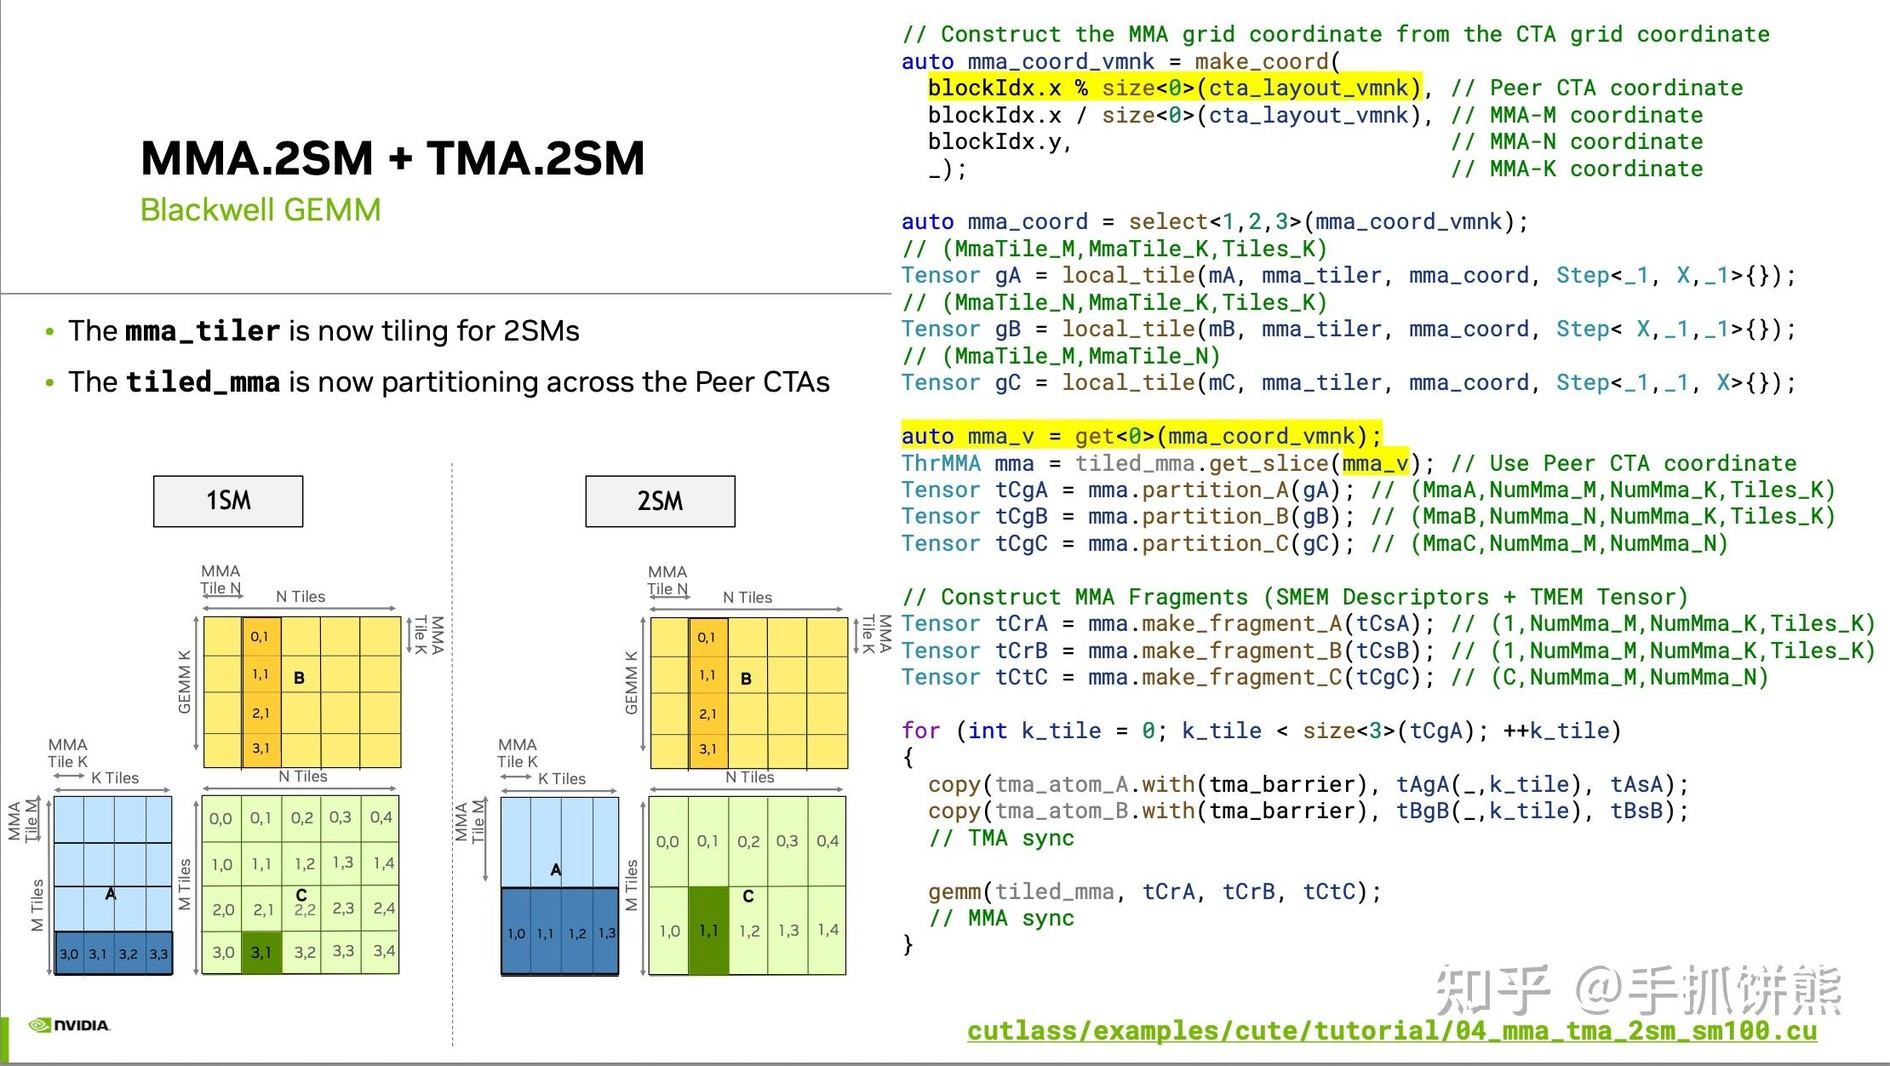
\includegraphics[width=0.9\textwidth]{figures/zhaoshangchun-01-tensor-core-programming/fig-38.jpg}
\end{figure}

这一页通过图示，进一步阐明了 \texttt{MMA.\allowbreak{}2\allowbreak{}SM} 模式下\textbf{计算任务的切分（Tiling）逻辑}，并将它与传统的 \texttt{1\allowbreak{}SM} 模式进行了对比。这对于理解 \texttt{2\allowbreak{}SM} 模式的性能优势来源至关重要。

右侧的图示是本页的核心。上半部分的 “1\allowbreak{}SM” 图展示了传统 GEMM 的切分方式：整个 GEMM 问题被划分为一个个独立的 tile（例如 \texttt{3,\allowbreak{}1}），每个 tile 由一个 CTA（或一个 SM）独立完成。这种方式简单直观，但当单个 tile 的尺寸受到 SMEM 或寄存器容量限制时，计算的并行粒度也相应受限。

下半部分的 “2\allowbreak{}SM” 图则展示了新的切分范式。在这里，\textbf{两个物理上相邻的 tile（例如 \texttt{0,\allowbreak{}1} 和 \texttt{1,\allowbreak{}1}）在逻辑上被组合成一个更大的 MMA tile}。这个更大的 tile 由一个 2-CTA 组共同负责。从 M 维度上看，这个 MMA tile 的高度是单个 SM tile 的两倍。图中的 \texttt{MMA Tile M} 箭头横跨了两个原始 tile，清晰地表明了这一点。这种设计的直接好处是\textbf{增大了单次 MMA 操作的规模}。更大的 MMA 操作意味着更高的计算访存比，因为启动一次计算所需处理的数据量更多，而控制开销（指令分发、同步等）可以被更好地摊销。

代码层面，这种变化体现在 \texttt{mma\_\allowbreak{}tiler} 和 \texttt{tiled\_\allowbreak{}mma} 的配置上。如注释所说，\texttt{T\allowbreak{}h\allowbreak{}e\allowbreak{} \allowbreak{}m\allowbreak{}m\allowbreak{}a\allowbreak{}\_\allowbreak{}t\allowbreak{}i\allowbreak{}l\allowbreak{}e\allowbreak{}r\allowbreak{} \allowbreak{}i\allowbreak{}s\allowbreak{} \allowbreak{}n\allowbreak{}o\allowbreak{}w\allowbreak{} \allowbreak{}t\allowbreak{}i\allowbreak{}l\allowbreak{}i\allowbreak{}n\allowbreak{}g\allowbreak{} \allowbreak{}f\allowbreak{}o\allowbreak{}r\allowbreak{} \allowbreak{}2\allowbreak{}S\allowbreak{}M\allowbreak{}s}，这意味着 \texttt{mma\_\allowbreak{}tiler} 在定义 tile 划分时，其 M 维度的步长（stride）会是单个 SM tile 的两倍。相应地，\texttt{T\allowbreak{}h\allowbreak{}e\allowbreak{} \allowbreak{}t\allowbreak{}i\allowbreak{}l\allowbreak{}e\allowbreak{}d\allowbreak{}\_\allowbreak{}m\allowbreak{}m\allowbreak{}a\allowbreak{} \allowbreak{}i\allowbreak{}s\allowbreak{} \allowbreak{}n\allowbreak{}o\allowbreak{}w\allowbreak{} \allowbreak{}p\allowbreak{}a\allowbreak{}r\allowbreak{}t\allowbreak{}i\allowbreak{}t\allowbreak{}i\allowbreak{}o\allowbreak{}n\allowbreak{}i\allowbreak{}n\allowbreak{}g\allowbreak{} \allowbreak{}a\allowbreak{}c\allowbreak{}r\allowbreak{}o\allowbreak{}s\allowbreak{}s\allowbreak{} \allowbreak{}t\allowbreak{}h\allowbreak{}e\allowbreak{} \allowbreak{}P\allowbreak{}e\allowbreak{}e\allowbreak{}r\allowbreak{} \allowbreak{}C\allowbreak{}T\allowbreak{}A\allowbreak{}s}，\texttt{tiled\_\allowbreak{}mma} 对象内部的逻辑会处理这种跨 CTA 的数据和计算划分。当 \texttt{get\_\allowbreak{}slice(0)} 和 \texttt{get\_\allowbreak{}slice(1)} 分别被调用时，它会返回对应 leader CTA 和 follower CTA 各自的计算任务视图。

\texttt{MMA.\allowbreak{}2\allowbreak{}SM} 模式的引入是 Blackwell 架构追求更高算术强度（arithmetic intensity）的体现。通过硬件支持，它打破了单个 SM 资源的限制，允许开发者定义出更大、更高效的计算粒度。这对于那些\textbf{计算密集型（compute-bound）}的 GEMM 问题尤其有利。然而，这也要求开发者（或如 Cu\allowbreak{}Te 这样的库）必须精确地管理跨 SM 的协作。例如，两个 CTA 需要通过 SMEM 或 L1/\allowbreak{}L2 缓存共享部分输入数据（如矩阵 B 的 tile），并最终将各自的累加结果合并（或直接写入到分布式的 TMEM 中）。Cu\allowbreak{}Te 的 \texttt{Tiled\allowbreak{}MMA} 正是为此而设计，它将这些复杂的协同细节抽象化，使得上层代码依然保持相对简洁。

\textbf{第 39 页：Blackwell GEMM 示例代码解析 - Leader CTA 与数据流}

\begin{figure}[H]\centering
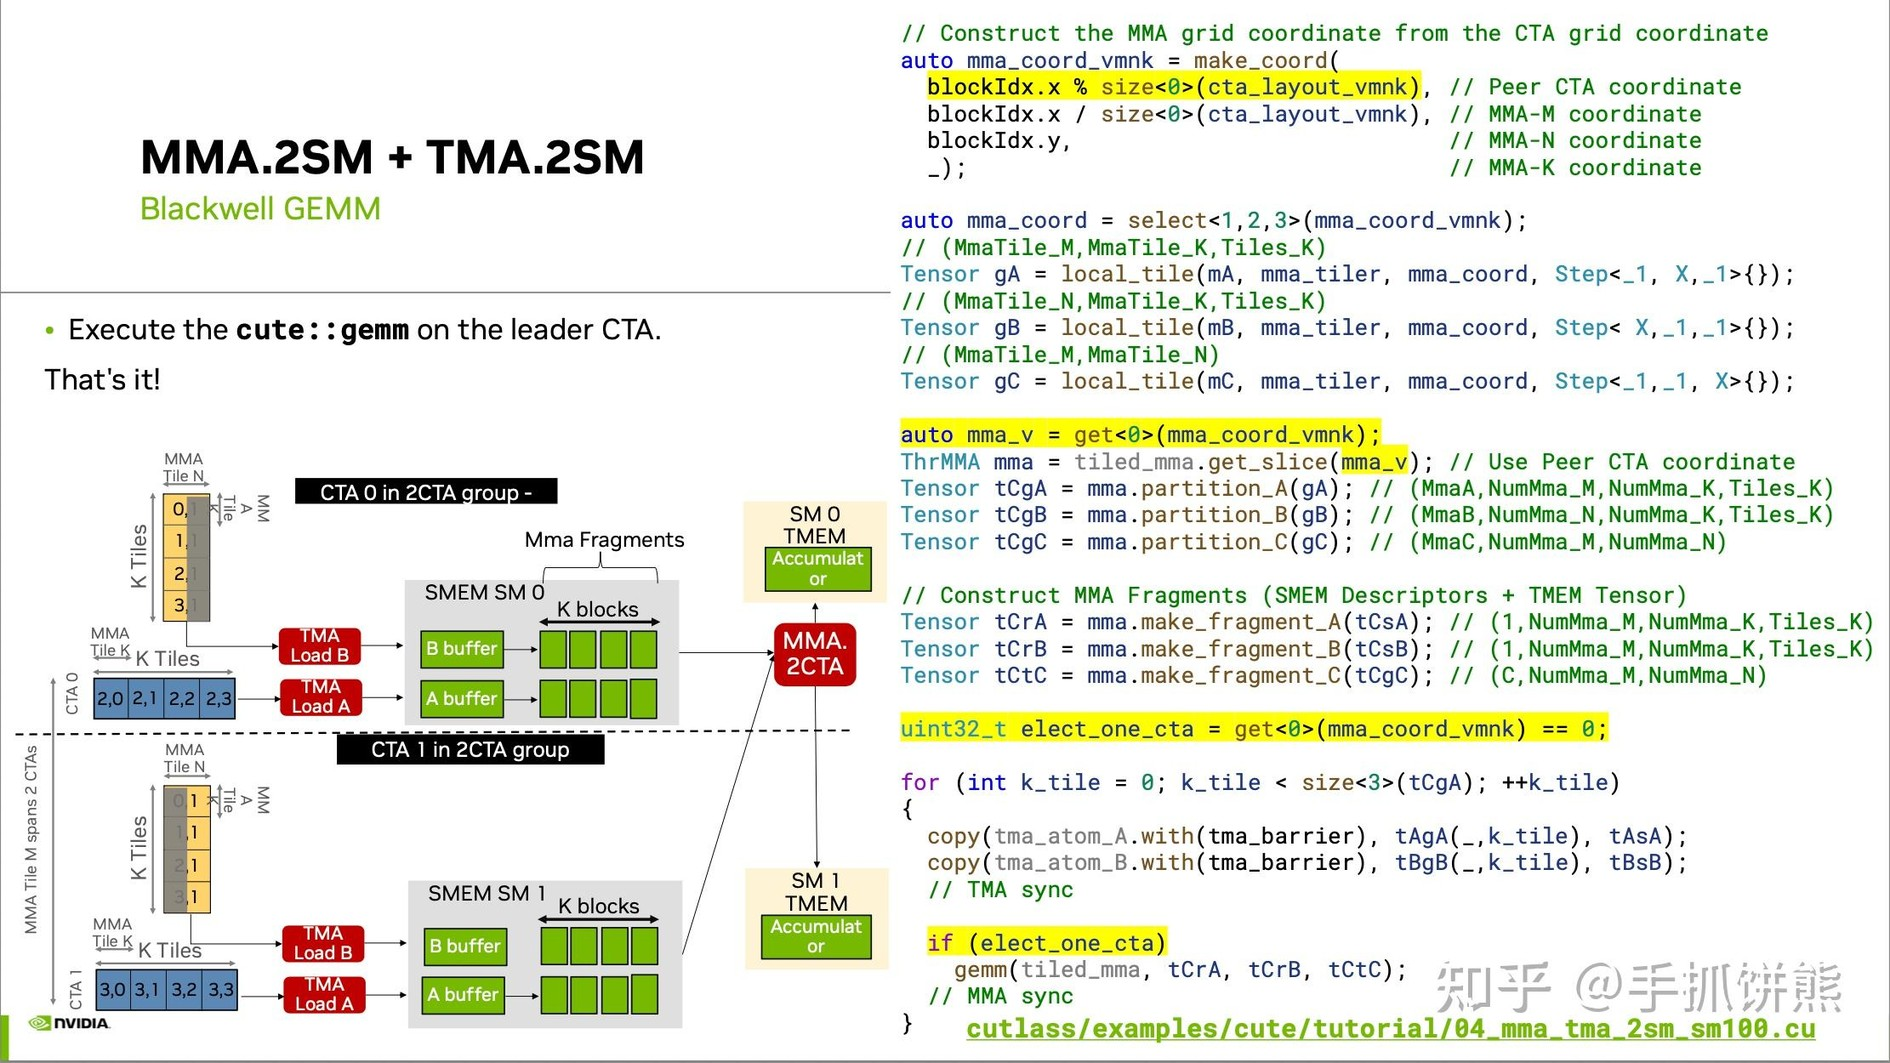
\includegraphics[width=0.9\textwidth]{figures/zhaoshangchun-01-tensor-core-programming/fig-39.jpg}
\end{figure}

这是 \texttt{MMA.\allowbreak{}2\allowbreak{}SM} 示例代码分析的最后一部分，揭示了 2-CTA 组中\textbf{如何通过选举“Leader CTA”来避免重复计算}，并给出了一个 \texttt{2\allowbreak{}SM} 模式下完整的数据流示意图。

代码中最核心的改动是增加了 \texttt{if (elect\_\allowbreak{}one\_\allowbreak{}cta)} 这个条件判断。\texttt{elect\_\allowbreak{}one\_\allowbreak{}cta} 变量通过 \texttt{g\allowbreak{}e\allowbreak{}t\allowbreak{}<\allowbreak{}0\allowbreak{}>\allowbreak{}(\allowbreak{}m\allowbreak{}m\allowbreak{}a\allowbreak{}\_\allowbreak{}c\allowbreak{}o\allowbreak{}o\allowbreak{}r\allowbreak{}d\allowbreak{}\_\allowbreak{}v\allowbreak{}m\allowbreak{}n\allowbreak{}k\allowbreak{})\allowbreak{} \allowbreak{}=\allowbreak{}=\allowbreak{} \allowbreak{}0} 来判断当前 CTA 是否为 2-CTA 组中的 leader（Peer ID 为 0）。只有 leader CTA 才会执行 \texttt{gemm(.\allowbreak{}.\allowbreak{}.\allowbreak{})} 函数。这看似奇怪——为什么两个 CTA 协作，却只有一个在工作？答案在于 \texttt{gemm} 函数内部的 \texttt{Tiled\allowbreak{}MMA} 对象已经封装了 \texttt{MMA.\allowbreak{}2\allowbreak{}SM} 的逻辑。当 leader CTA 调用 \texttt{gemm} 时，它发出的 \texttt{t\allowbreak{}c\allowbreak{}g\allowbreak{}e\allowbreak{}n\allowbreak{}0\allowbreak{}5\allowbreak{}.\allowbreak{}m\allowbreak{}m\allowbreak{}a\allowbreak{}.\allowbreak{}c\allowbreak{}t\allowbreak{}a\allowbreak{}\_\allowbreak{}g\allowbreak{}r\allowbreak{}o\allowbreak{}u\allowbreak{}p\allowbreak{}:\allowbreak{}:\allowbreak{}2\allowbreak{}.\allowbreak{}*} PTX 指令\textbf{会自动触发其伙伴 CTA（follower）上的 Tensor Core 协同进行计算}。因此，这个 \texttt{if} 语句的真正作用是\textbf{防止 follower CTA 也独立地发出相同的 MMA 指令，从而导致计算被重复执行两次}。这是一种高效的命令分发机制，由一个 leader 统一调度，两个 SM 共同执行。

右侧的图示生动地描绘了 \texttt{MMA.\allowbreak{}2\allowbreak{}SM} 模式下的完整数据流：

\begin{enumerate}
\item \textbf{数据加载 (TMA)}：CTA 0 和 CTA 1（分别位于 SM0 和 SM1）都参与数据加载。它们通过 TMA 从 GMEM 中读取各自负责的 A 矩阵和 B 矩阵的 tile，并存入各自的 SMEM 中（\texttt{A buffer}, \texttt{B buffer}）。注意，B 矩阵的 tile 对于 M 维度的两个部分是共享的，因此两个 CTA 可能会加载相同的 B tile，或者通过 cluster 广播来共享。
\item \textbf{计算分片 (MMA Fragments)}：两个 CTA 根据 \texttt{Tiled\allowbreak{}MMA} 的分区策略，从 SMEM 中构建出 MMA 指令所需的输入分片（\texttt{Mma Fragments}）。
\item \textbf{协同计算 (MMA.2\allowbreak{}CTA)}：Leader CTA (CTA 0) 发出 \texttt{gemm} 指令。该指令驱动 SM0 和 SM1 上的 Tensor Core 同时开始工作。如图所示，\texttt{MMA Tile M} 的计算任务被分给了两个 SM，它们共同完成一次大的矩阵乘法累加。
\item \textbf{结果存储 (TMEM Accumulator)}：计算结果（累加值 C）被直接写入到分布在两个 SM 上的 TMEM 中。\texttt{TMEM Accumulator} 图示表明，结果 C 的一部分位于 SM0 的 TMEM，另一部分位于 SM1 的 TMEM。
\end{enumerate}

在 Hopper 中，CTA 之间虽然可以通过 cluster 共享数据，但计算本身是严格限制在 SM 内部的。而在 Blackwell 中，\textbf{计算本身也可以跨 SM 协作}，形成了 \texttt{TMA.\allowbreak{}2\allowbreak{}SM} (数据) + \texttt{MMA.\allowbreak{}2\allowbreak{}SM} (计算) 的双重协作模式。这种模式的工程影响是巨大的：它允许 CUTLASS 定义出两倍于以往的 M-tile 规模，极大地提升了算术强度和数据重用率，从而在不显著增加 SMEM 或寄存器压力的情况下，实现了更高的 GEMM 性能。同时，将累加器放在 TMEM 中，为后续复杂的 Epilogue 操作（如多层神经网络的激活、归一化等融合）释放了宝贵的寄存器资源，使得端到端的算子性能更上一层楼。

\subsection{\textbf{TMEM}累加器}

从第 40-49 页：主要介绍处理 TMEM 累加器和 Epilogue。在计算完成之后，累加器结果位于 TMEM 中。如何将其取出并写回到 GMEM，就是 Epilogue 阶段的核心任务。

\textbf{第 41 页：Blackwell TMEM and PTX}

\begin{figure}[H]\centering
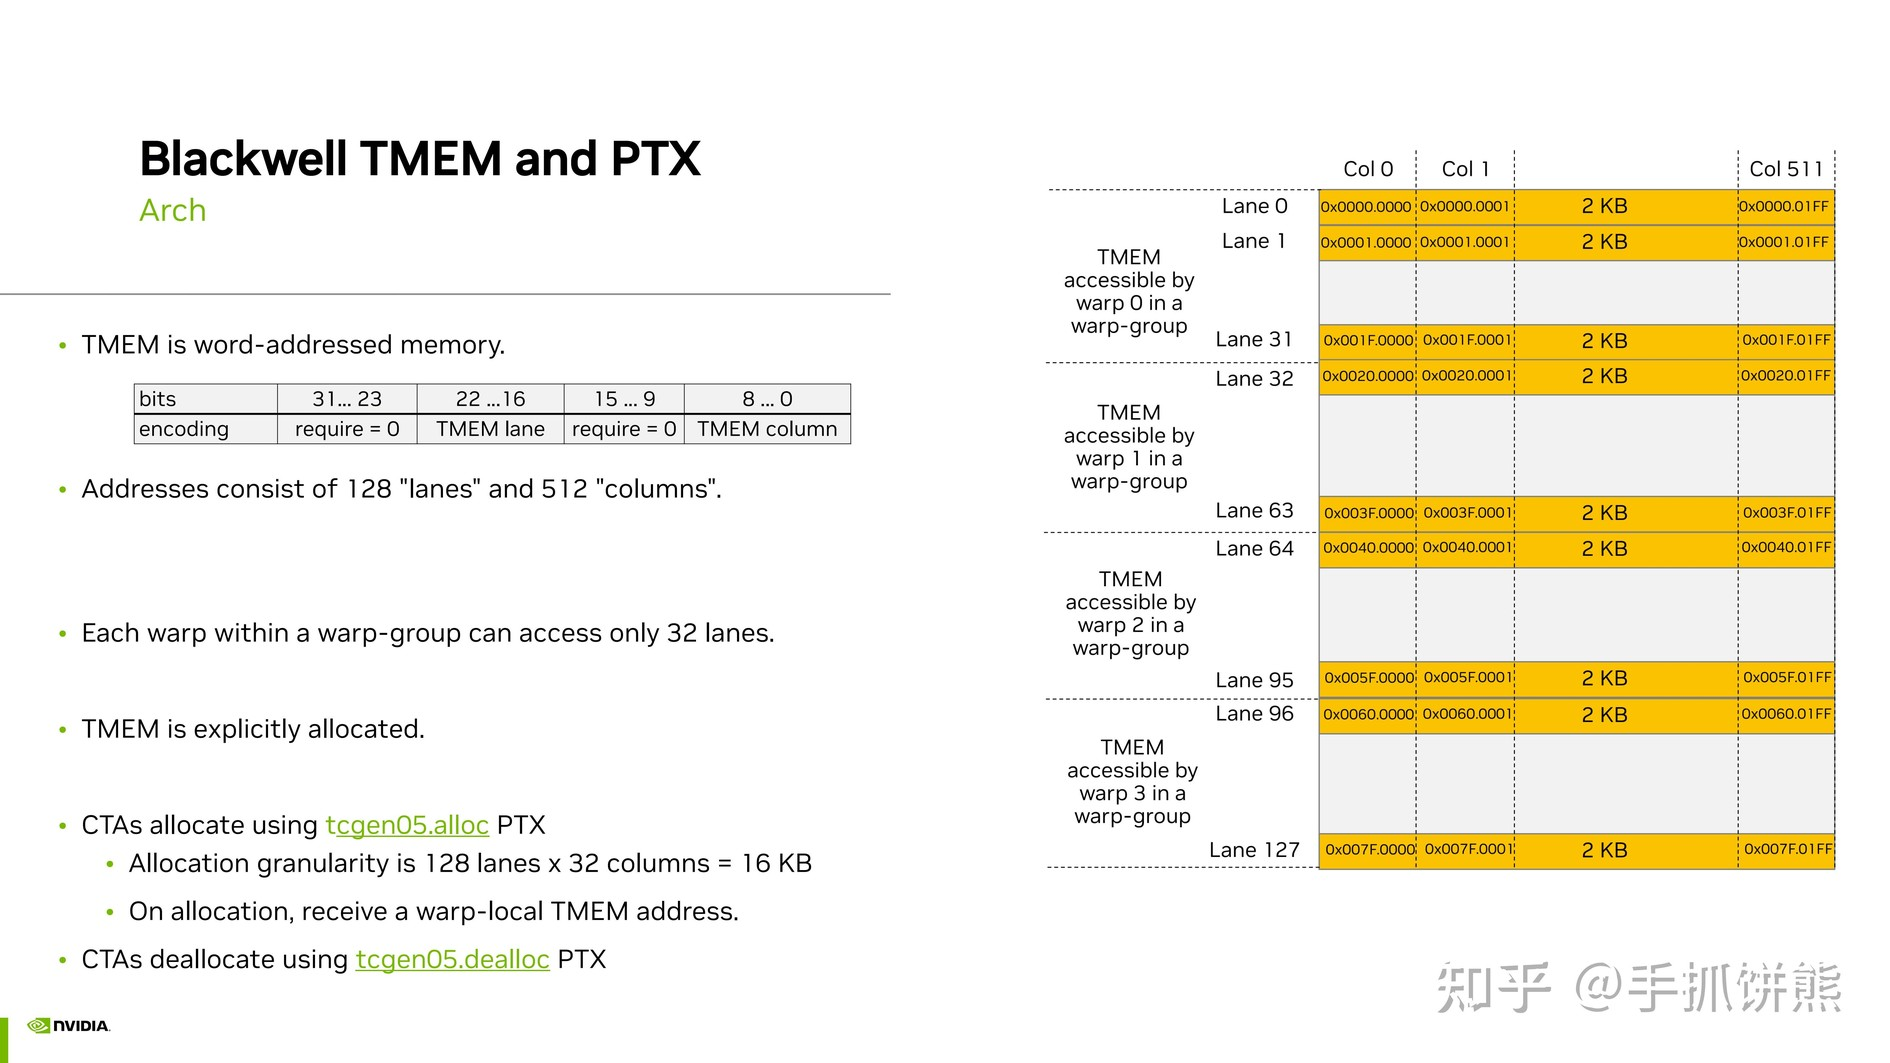
\includegraphics[width=0.9\textwidth]{figures/zhaoshangchun-01-tensor-core-programming/fig-40.jpg}
\end{figure}

这一页深入 TMEM 的寻址和分配细节：

\begin{itemize}
\item \textbf{寻址方式}：TMEM 是“字寻址（word-addressed）”的，地址由 128 个 \texttt{lane} 和 512 个 \texttt{column} 组成。一个 warpgroup（4个 warp）可以访问所有 lane，而单个 warp 只能访问 32 个 lane。
\item \textbf{分配/\allowbreak{}释放}：需要使用 \texttt{tcgen05.\allowbreak{}alloc} 和 \texttt{tcgen05.\allowbreak{}dealloc} PTX 指令进行显式管理。分配的粒度是 16 KB（128 lanes x 32 columns）。
\item \textbf{warp-local 地址}：\texttt{alloc} 指令返回的是一个 warp-local 的地址，这意味着不同 warp 获取的地址值可能不同，但它们指向同一个分配的 TMEM 块。
\end{itemize}

TMEM 的这些底层细节决定了它的使用方式和编程模型的复杂性。

\begin{itemize}
\item \textbf{非传统内存}：TMEM 不是我们熟悉的线性地址空间。它的地址编码 (\texttt{lane}, \texttt{column}) 意味着我们不能用简单的指针算术来访问数据。必须使用专门的指令和预定义的布局。
\item \textbf{手动内存管理的回归}：在高级语言中，我们已经习惯了自动内存管理。但在追求极致性能的 GPU 内核编程中，手动管理 TMEM 这样的关键资源是必要的。这要求开发者对内核的生命周期有精确的控制。
\item \textbf{集合操作的必要性}：由于地址是 warp-local 的，且单个 warp 无法访问全部 TMEM，所有对 TMEM 的操作都必须是 warpgroup 范围内的集体操作。这再次强调了在 Blackwell 编程中，\texttt{warpgroup} 是基本的操作单元。
\end{itemize}

\textbf{第 42 页：Blackwell TMEM Tensors and Ops}

\begin{figure}[H]\centering
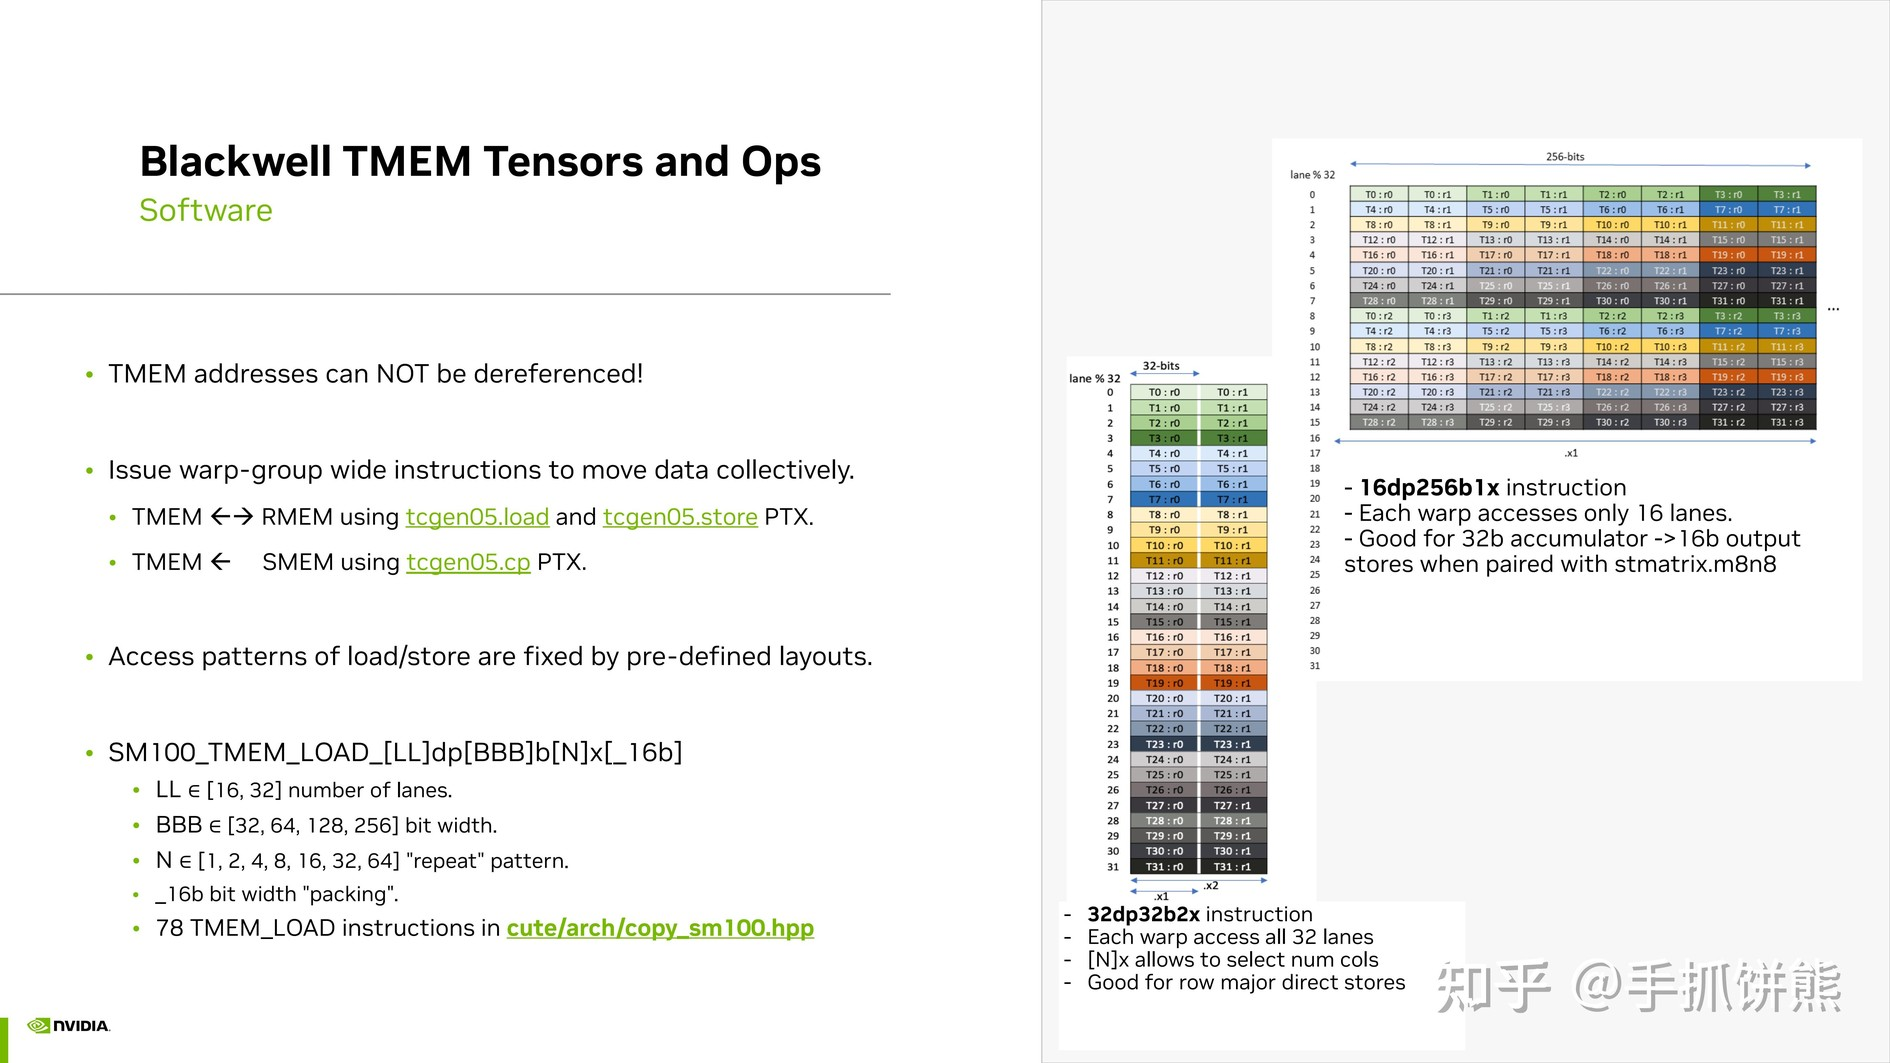
\includegraphics[width=0.9\textwidth]{figures/zhaoshangchun-01-tensor-core-programming/fig-41.jpg}
\end{figure}

\begin{itemize}
\item \textbf{TMEM 地址不可解引用}：这是一个核心限制！你不能像 C 语言中那样对一个 TMEM 地址指针做 \texttt{*ptr} 操作。
\item \textbf{数据移动指令}：
\item \texttt{TMEM ↔ RMEM} (寄存器)：使用 \texttt{tcgen05.\allowbreak{}load} 和 \texttt{tcgen05.\allowbreak{}store}。
\item \texttt{TMEM ↔ SMEM} (共享内存)：使用 \texttt{tcgen05.\allowbreak{}cp}。
\item \textbf{固定的访问模式}：这些 \texttt{load}/\allowbreak{}\texttt{store} 指令的访问模式是固定的，由硬件预先定义。例如 \texttt{S\allowbreak{}M\allowbreak{}1\allowbreak{}0\allowbreak{}0\allowbreak{}\_\allowbreak{}T\allowbreak{}M\allowbreak{}E\allowbreak{}M\allowbreak{}\_\allowbreak{}L\allowbreak{}O\allowbreak{}A\allowbreak{}D\allowbreak{}\_\allowbreak{}[\allowbreak{}L\allowbreak{}L\allowbreak{}]\allowbreak{}d\allowbreak{}p\allowbreak{}[\allowbreak{}B\allowbreak{}B\allowbreak{}B\allowbreak{}]\allowbreak{}b\allowbreak{}[\allowbreak{}N\allowbreak{}]\allowbreak{}x}，其中 \texttt{LL} 是 lane 数，\texttt{BBB} 是位宽，\texttt{N} 是重复次数。Cu\allowbreak{}Te 在 \texttt{cute/\allowbreak{}arch/\allowbreak{}copy\_\allowbreak{}sm100.\allowbreak{}hpp} 中为这些指令提供了抽象。
\end{itemize}

TMEM 的这种“黑盒”特性，使得直接使用它变得异常困难。

\begin{itemize}
\item \textbf{编程范式的转变}：我们必须放弃“指针-解引用”的思维定式，转向一种基于“指令-布局”的声明式编程范式。我们能做的，是选择一个合适的 \texttt{load}/\allowbreak{}\texttt{store} 指令（它隐含了一种访问布局），然后让硬件去执行它。
\item \textbf{布局（Layout）是关键}：因为访问模式是固定的，所以成功的关键在于，如何组织 TMEM 中的数据布局，使其能够匹配某个 \texttt{load}/\allowbreak{}\texttt{store} 指令的模式。这就是 Cu\allowbreak{}Te 的 \texttt{Layout} 和 \texttt{Tensor} 抽象发挥巨大价值的地方。
\item \textbf{指令选择的艺术}：幻灯片中举了两个例子：\texttt{32dp32b2x} 指令适合行主序的直接存储；而 \texttt{16dp256b1x} 适合将 32 位的累加器结果转换成 16 位输出。选择哪条指令，取决于你的 Epilogue 需要做什么。这是一个需要经验和实验的调优过程。
\end{itemize}

\textbf{第 43 页：TMEM Tensor 和 Tiled\allowbreak{}Copy}

\begin{figure}[H]\centering
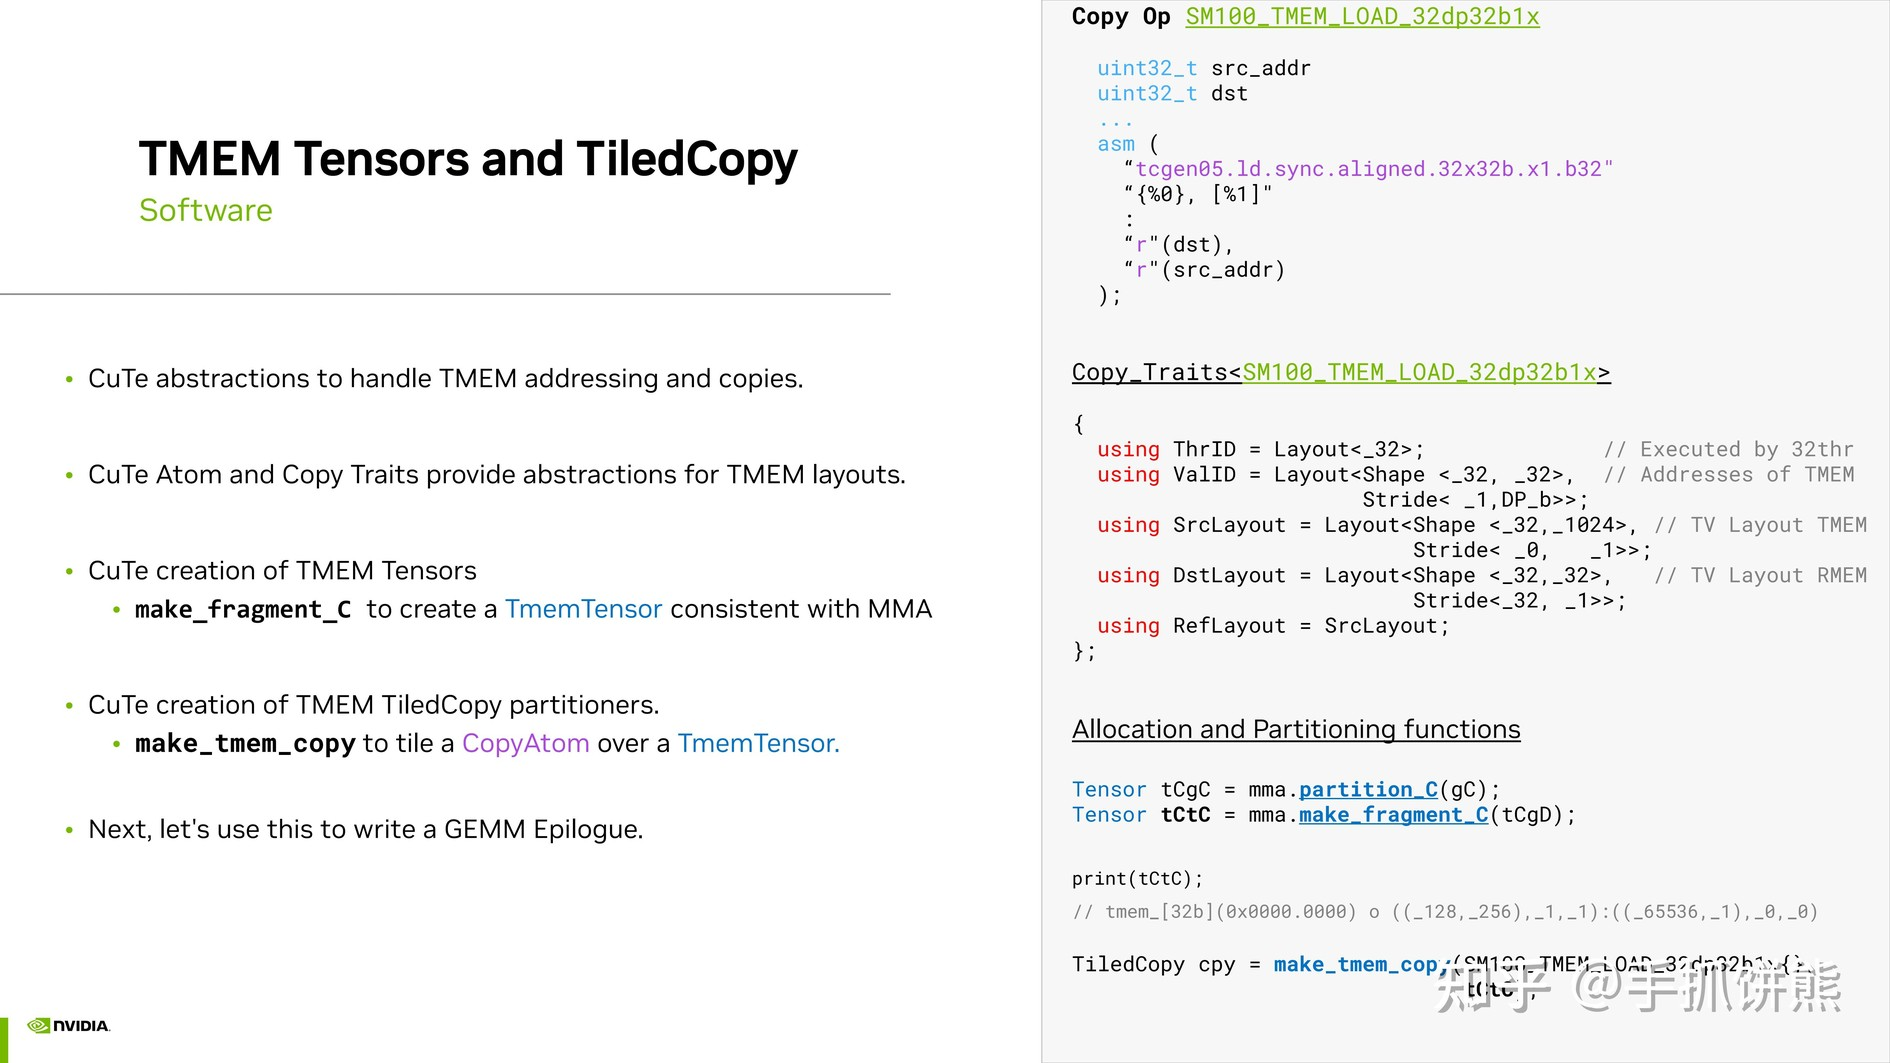
\includegraphics[width=0.9\textwidth]{figures/zhaoshangchun-01-tensor-core-programming/fig-42.jpg}
\end{figure}

\begin{itemize}
\item \textbf{Cu\allowbreak{}Te 的抽象}：Cu\allowbreak{}Te 提供了 \texttt{Atom}, \texttt{Copy\_\allowbreak{}Traits}, \texttt{Tiled\allowbreak{}Copy} 等一系列抽象来封装 TMEM 的复杂性。
\item \textbf{\texttt{make\_\allowbreak{}fragment\_\allowbreak{}C}}：这个函数不仅为 MMA 准备 C 的片段，它创建的 \texttt{t\allowbreak{}Ct\allowbreak{}C} 本身就是一个 \texttt{Tmem\allowbreak{}Tensor}，其布局与 MMA 的输出布局完全匹配。
\item \textbf{\texttt{make\_\allowbreak{}tmem\_\allowbreak{}copy}}：这是一个新的工厂函数，它接收一个 TMEM 的 \texttt{Copy\allowbreak{}Atom}（例如 \texttt{S\allowbreak{}M\allowbreak{}1\allowbreak{}0\allowbreak{}0\allowbreak{}\_\allowbreak{}T\allowbreak{}M\allowbreak{}E\allowbreak{}M\allowbreak{}\_\allowbreak{}L\allowbreak{}O\allowbreak{}A\allowbreak{}D\allowbreak{}\_\allowbreak{}3\allowbreak{}2\allowbreak{}d\allowbreak{}p\allowbreak{}3\allowbreak{}2\allowbreak{}b\allowbreak{}1\allowbreak{}x}）和一个 \texttt{Tmem\allowbreak{}Tensor} (\texttt{t\allowbreak{}Ct\allowbreak{}C})，然后创建一个 \texttt{Tiled\allowbreak{}Copy} 对象。这个 \texttt{Tiled\allowbreak{}Copy} 对象知道如何将 \texttt{Copy\allowbreak{}Atom} 平铺到整个 \texttt{Tmem\allowbreak{}Tensor} 上，以实现完整的数据拷贝。
\end{itemize}

Cu\allowbreak{}Te 在这里扮演了“翻译官”的角色，将程序员的“意图”翻译成硬件能听懂的“指令”。

\begin{itemize}
\item \textbf{从 \texttt{Tensor} 到 \texttt{Tensor} 的拷贝}：通过 \texttt{Tiled\allowbreak{}Copy}，开发者可以像操作普通 \texttt{Tensor} 一样，发起一个从 TMEM \texttt{Tensor} 到 RMEM \texttt{Tensor} 或 SMEM \texttt{Tensor} 的拷贝，而无需关心底层的 \texttt{lane}, \texttt{column} 寻址和 PTX 指令。
\item \textbf{自动化布局匹配}：\texttt{make\_\allowbreak{}tmem\_\allowbreak{}copy} 的过程实际上是在解决一个匹配问题：如何用 \texttt{Copy\allowbreak{}Atom} 定义的小块拷贝模式，去完整地、不重不漏地覆盖 \texttt{Tmem\allowbreak{}Tensor} 定义的大块数据。Cu\allowbreak{}Te 的 \texttt{Tiled\allowbreak{}Copy} 算法会自动解决这个问题。
\item \textbf{Epilogue 的构建块}：\texttt{Tiled\allowbreak{}Copy} 是构建 Blackwell 高性能 Epilogue 的核心构件。通过组合不同的 \texttt{Tiled\allowbreak{}Copy}，我们可以实现从 TMEM 加载数据，在 RMEM 中进行各种计算（如激活函数、类型转换），然后写回到 GMEM 的复杂流水线。
\end{itemize}

\subsection{完整的 TMEM Epilogue 流程}

从44-49页是一个连贯的示例，展示了如何为之前的 GEMM 内核添加一个 Epilogue，将 TMEM 中的累加结果写回全局内存。

\textbf{第 44 页：TMEM Epilogue - 问题与分区总览}

\begin{figure}[H]\centering
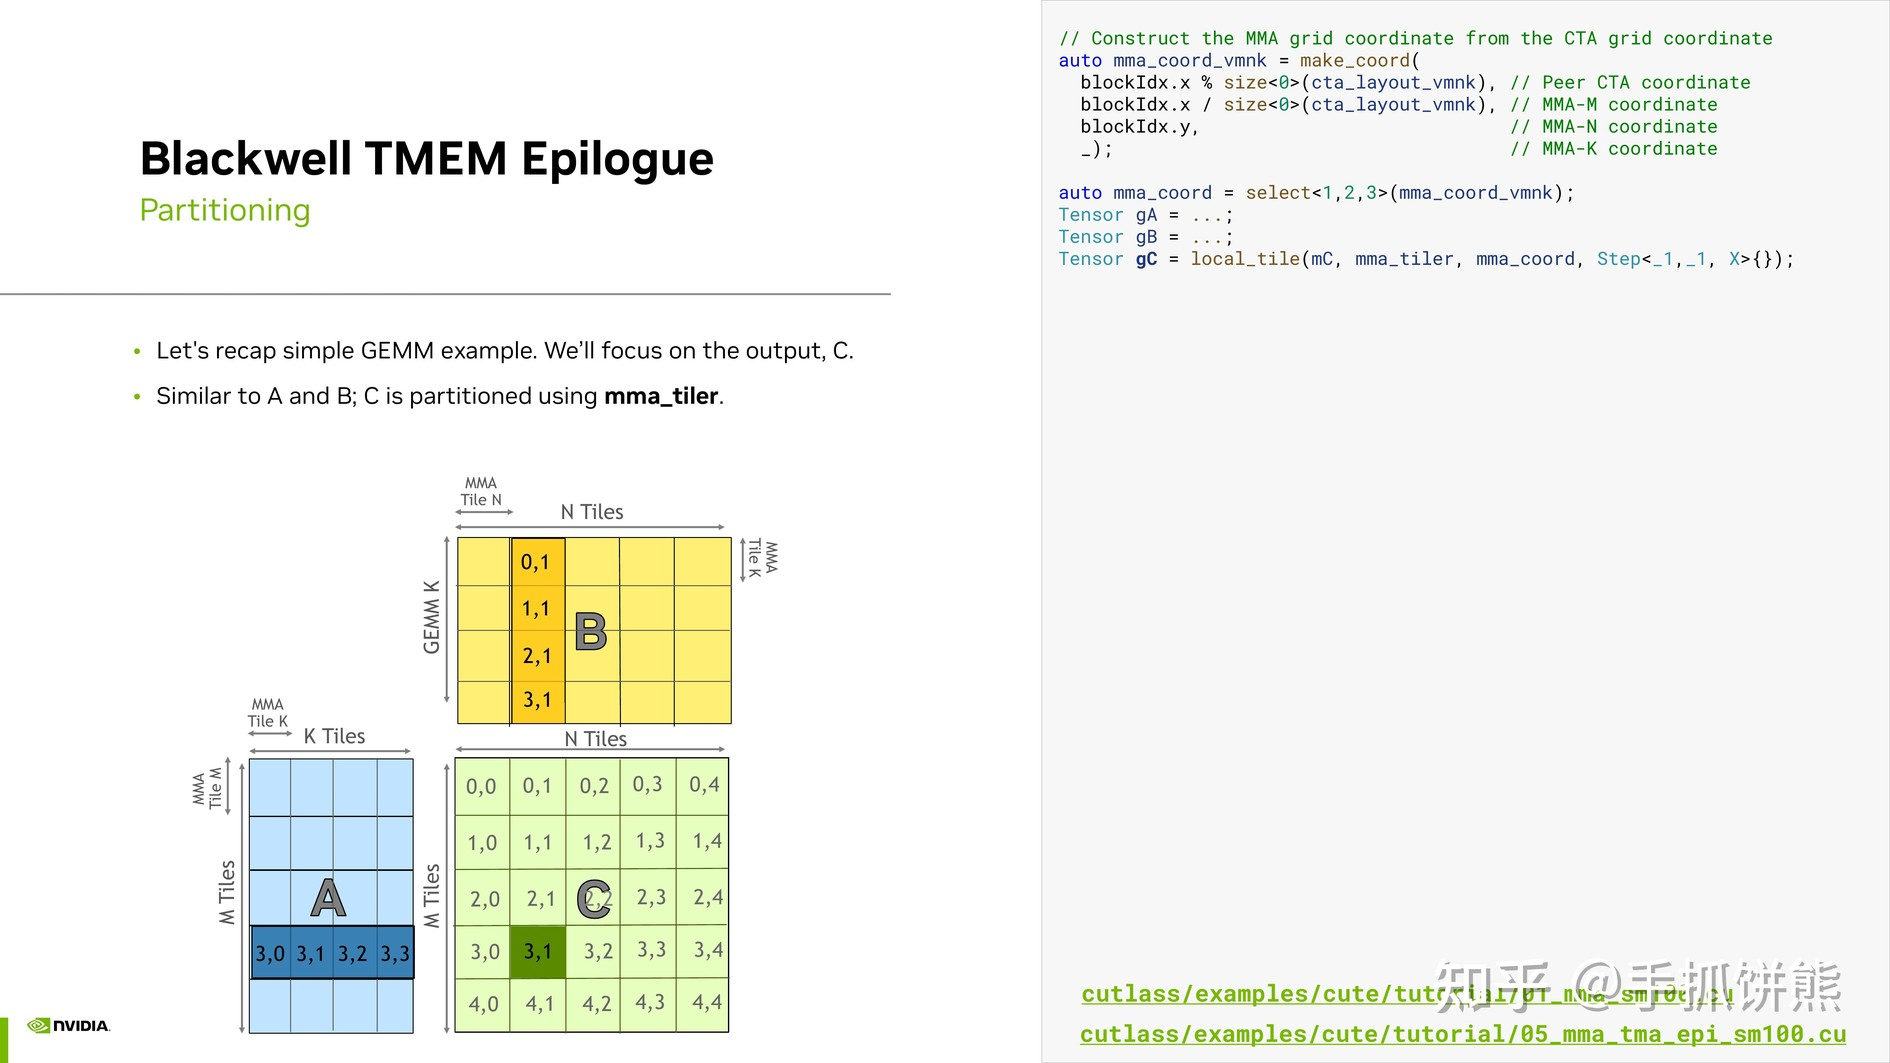
\includegraphics[width=0.9\textwidth]{figures/zhaoshangchun-01-tensor-core-programming/fig-43.jpg}
\end{figure}

这张幻灯片开启了对 Blackwell 架构下 \textbf{TMEM Epilogue} 的讨论。Epilogue 是指在 GEMM 主循环计算完成后，处理累加结果（矩阵 C）并写回全局内存（Global Memory）的阶段。在 Blackwell 中，由于累加器（Accumulator）可以直接存在于新引入的 TMEM 中，因此 Epilogue 的流程也发生了深刻变化。

首先，幻灯片回顾了 CUTLASS/\allowbreak{}Cu\allowbreak{}Te 中对矩阵进行分区的基本思想。与输入矩阵 A 和 B 类似，\textbf{输出矩阵 C 也被 \texttt{mma\_\allowbreak{}tiler} 在逻辑上划分为一个个小的 Tile}。每个 Tile 由一个或一组 Cooperative Thread Array (CTA) 负责计算和写回。这种分区是后续所有计算和数据移动的基础，它定义了问题的粒度。

代码部分展示了如何从 \texttt{block\allowbreak{}Idx}（CTA 在 Grid 中的坐标）计算出 \texttt{mma\_\allowbreak{}coord\_\allowbreak{}vmnk}。这是一个四维坐标，\textbf{精确地定义了当前 CTA 在整个 GEMM 问题中的位置}：

\begin{itemize}
\item \texttt{Peer CTA coordinate}：在同一个 2\allowbreak{}SM (Streaming Multiprocessor) MMA (Matrix Multiply-Accumulate) 指令组中的伙伴 CTA 索引。
\item \texttt{MMA-M coordinate}：在 M 维度上的 Tile 索引。
\item \texttt{MMA-N coordinate}：在 N 维度上的 Tile 索引。
\item \texttt{MMA-K coordinate}：在 K 维度上的 Tile 索引（在 Epilogue 中通常不使用）。通过 \texttt{select<1,\allowbreak{}2,\allowbreak{}3>}，我们提取出与 MMA 计算直接相关的 M 和 N 维度坐标，用于后续通过 \texttt{local\_\allowbreak{}tile} 从全局 C 矩阵（\texttt{m\allowbreak{}C}）中切分出当前 CTA 需要负责的逻辑分区 \texttt{g\allowbreak{}C}。这一步是连接宏观问题与微观计算的桥梁。
\end{itemize}

\textbf{第 45 页：TMEM Epilogue - CTA 本地视图与 TMEM 张量创建}

\begin{figure}[H]\centering
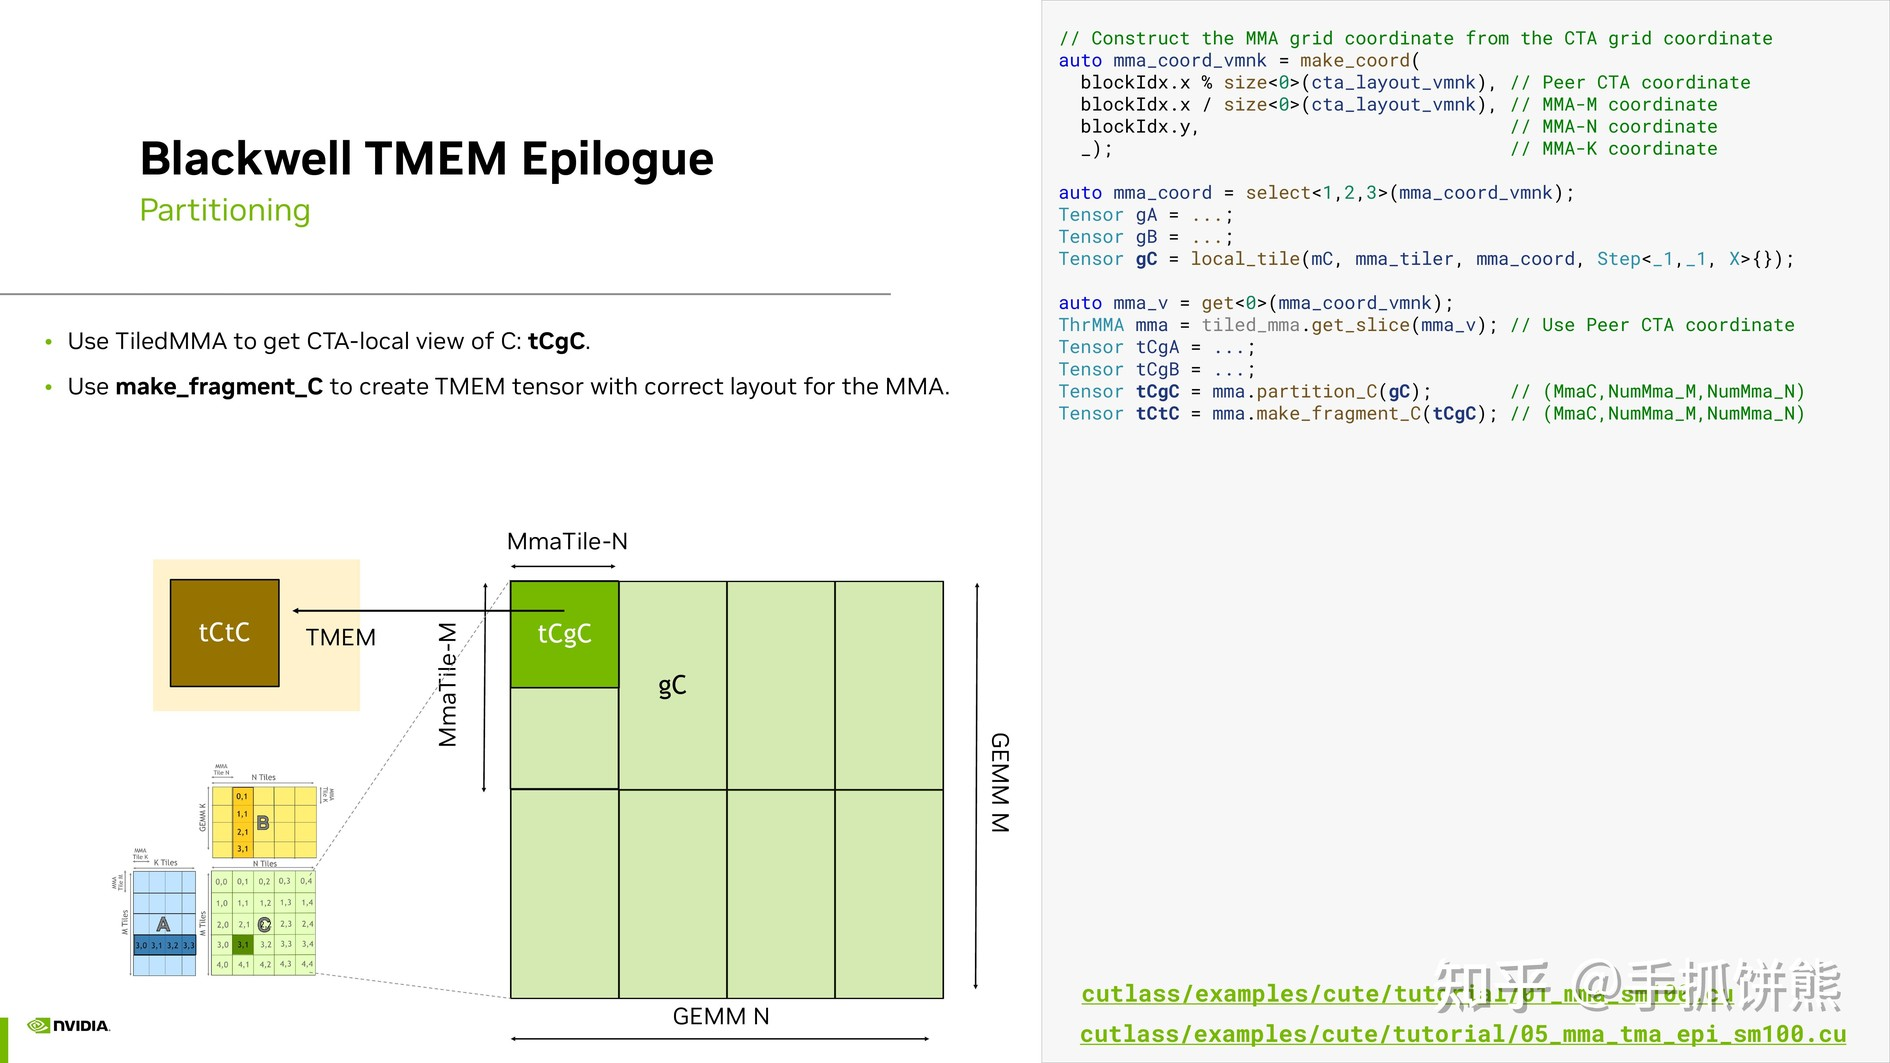
\includegraphics[width=0.9\textwidth]{figures/zhaoshangchun-01-tensor-core-programming/fig-44.jpg}
\end{figure}

在确定了全局分区 \texttt{g\allowbreak{}C} 后，第 45 页展示了如何将其进一步细化，并最终映射到 TMEM 上。这是 Epilogue 真正进入硬件抽象层的第一步。

代码中的 \texttt{t\allowbreak{}i\allowbreak{}l\allowbreak{}e\allowbreak{}d\allowbreak{}\_\allowbreak{}m\allowbreak{}m\allowbreak{}a\allowbreak{}.\allowbreak{}g\allowbreak{}e\allowbreak{}t\allowbreak{}\_\allowbreak{}s\allowbreak{}l\allowbreak{}i\allowbreak{}c\allowbreak{}e\allowbreak{}(\allowbreak{}m\allowbreak{}m\allowbreak{}a\allowbreak{}\_\allowbreak{}v\allowbreak{})} 是关键。这里的 \texttt{mma\_\allowbreak{}v} 是指 \texttt{Peer CTA coordinate}，它告诉 \texttt{Tiled\allowbreak{}MMA} 对象当前是哪个 CTA 在工作。\texttt{get\_\allowbreak{}slice} 返回一个 \texttt{Thr\allowbreak{}MMA} 对象，它封装了单个 CTA 在多 CTA 协作（如 2\allowbreak{}SM-MMA）中所扮演的角色和所需的数据视图。接着，\texttt{mma.\allowbreak{}partition\_\allowbreak{}C(g\allowbreak{}C)} 将全局分区 \texttt{g\allowbreak{}C} 转换为 \textbf{CTA 的本地视图 \texttt{t\allowbreak{}Cg\allowbreak{}C}}。\texttt{t\allowbreak{}Cg\allowbreak{}C} 仍然指向全局内存，但其布局和元数据已经根据当前 CTA 的视角进行了调整。

最重要的一步是 \texttt{m\allowbreak{}m\allowbreak{}a\allowbreak{}.\allowbreak{}m\allowbreak{}a\allowbreak{}k\allowbreak{}e\allowbreak{}\_\allowbreak{}f\allowbreak{}r\allowbreak{}a\allowbreak{}g\allowbreak{}m\allowbreak{}e\allowbreak{}n\allowbreak{}t\allowbreak{}\_\allowbreak{}C\allowbreak{}(\allowbreak{}t\allowbreak{}C\allowbreak{}g\allowbreak{}C\allowbreak{})}，它创建了 \textbf{TMEM 张量 \texttt{t\allowbreak{}Ct\allowbreak{}C}}。这一步并不涉及实际的数据拷贝，而是\textbf{在逻辑上创建了一个位于 TMEM 中的 Tensor 对象}，该对象的布局（Layout）被精心设计，以完美匹配后续 MMA 指令的累加操作。\texttt{t\allowbreak{}Ct\allowbreak{}C} 代表了最终 GEMM 计算结果在 TMEM 中的“容器”。与 Hopper 及更早架构将累加结果放在寄存器（RMEM）中不同，Blackwell \textbf{直接将 TMEM 作为累加器的主要存储位置}，这极大地增加了累加器的容量，减少了寄存器压力，为更大规模的 MMA Tile 和更复杂的 Epilogue 融合操作提供了可能。

\textbf{第 46 页：TMEM Epilogue - 作为累加器的 TMEM}

\begin{figure}[H]\centering
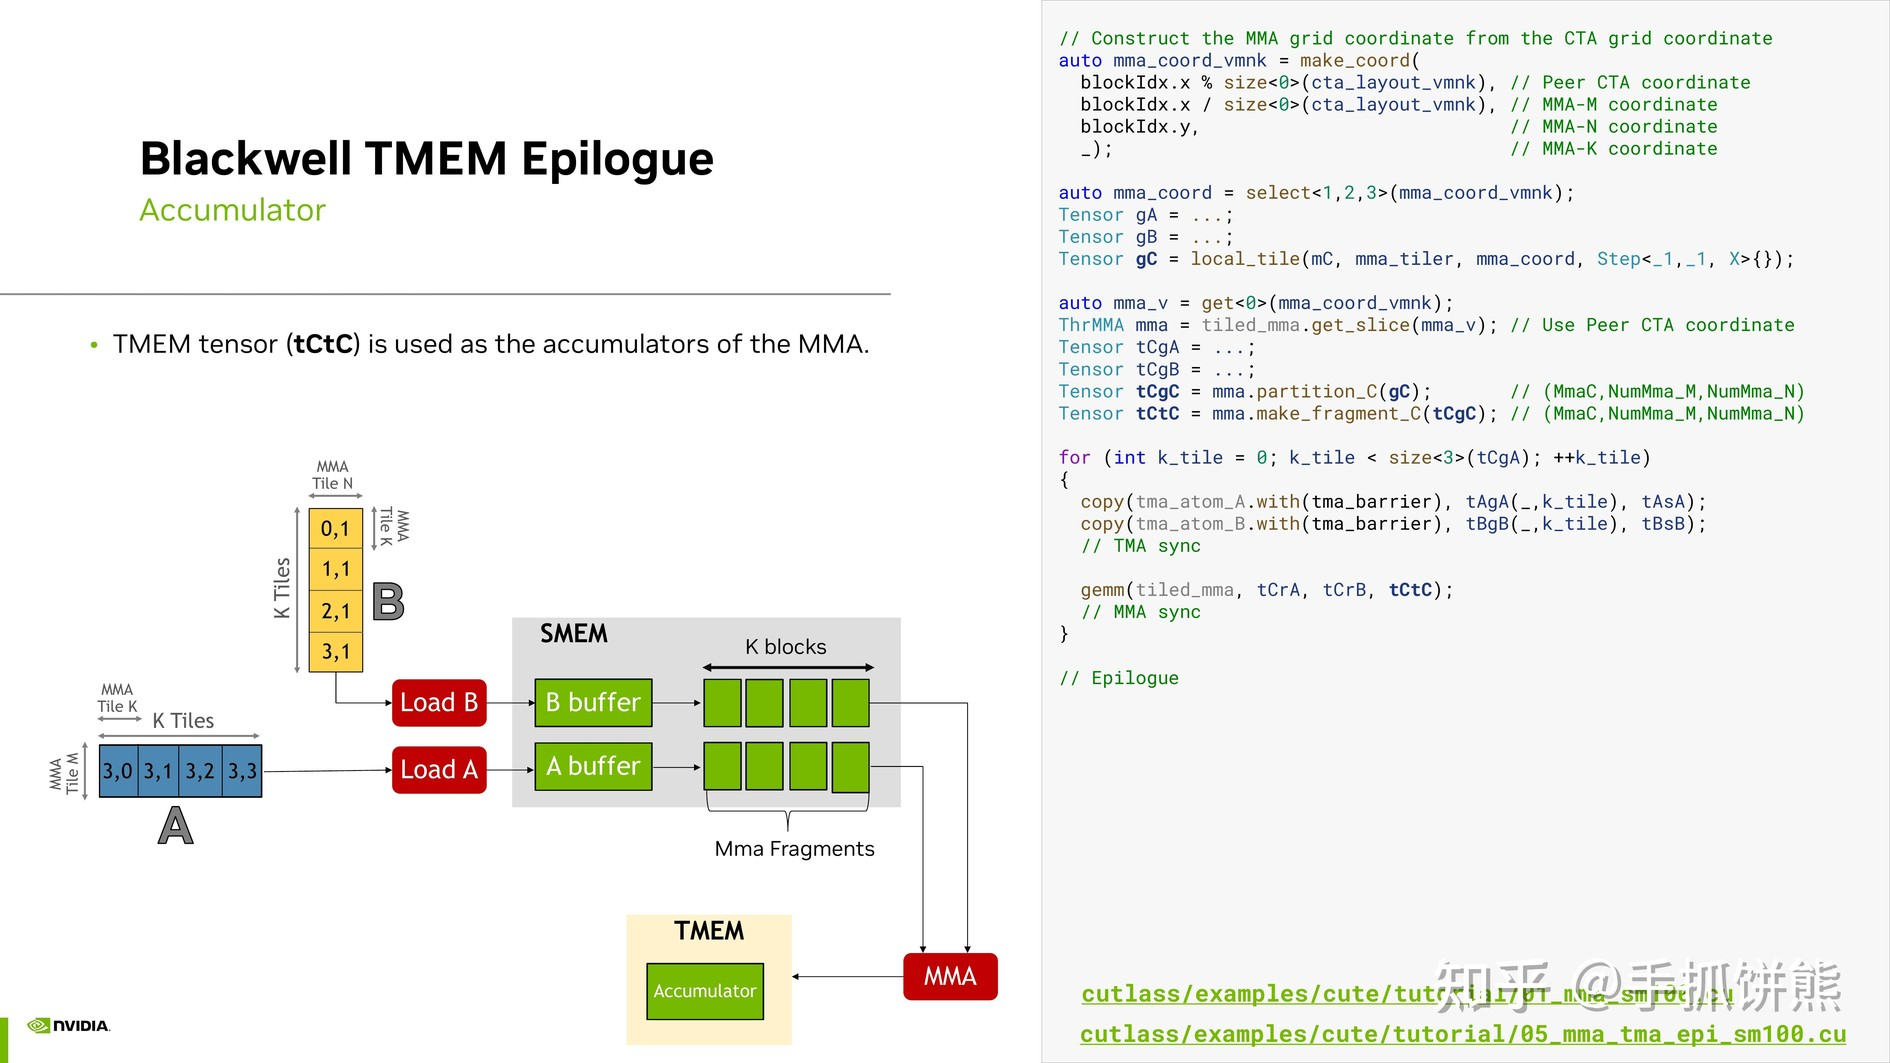
\includegraphics[width=0.9\textwidth]{figures/zhaoshangchun-01-tensor-core-programming/fig-45.jpg}
\end{figure}

第 46 页的图示和代码清晰地揭示了 \texttt{t\allowbreak{}Ct\allowbreak{}C} 的核心作用：\textbf{它在 \texttt{gemm} 主循环中直接作为累加器使用}。

在 \texttt{for} 循环内部，\texttt{g\allowbreak{}e\allowbreak{}m\allowbreak{}m\allowbreak{}(\allowbreak{}t\allowbreak{}i\allowbreak{}l\allowbreak{}e\allowbreak{}d\allowbreak{}\_\allowbreak{}m\allowbreak{}m\allowbreak{}a\allowbreak{},\allowbreak{} \allowbreak{}t\allowbreak{}C\allowbreak{}r\allowbreak{}A\allowbreak{},\allowbreak{} \allowbreak{}t\allowbreak{}C\allowbreak{}r\allowbreak{}B\allowbreak{},\allowbreak{} \allowbreak{}t\allowbreak{}C\allowbreak{}t\allowbreak{}C\allowbreak{})} 函数调用执行了核心的矩阵乘加运算。这里的 \texttt{t\allowbreak{}Cr\allowbreak{}A} 和 \texttt{t\allowbreak{}Cr\allowbreak{}B} 是分别来自 SMEM 的 A 和 B 矩阵的分片（Fragment），而 \texttt{t\allowbreak{}Ct\allowbreak{}C} 则是那个在 TMEM 中的累加器张量。每一轮 K 循环，\texttt{tcgen05.\allowbreak{}mma} 指令都会从 SMEM 中读取 A 和 B 的数据，与 \texttt{t\allowbreak{}Ct\allowbreak{}C} 中的当前值进行累加，并将新结果写回 \texttt{t\allowbreak{}Ct\allowbreak{}C}。

图示非常直观地展示了这个数据流：

\begin{enumerate}
\item \textbf{数据加载}：通过 \texttt{copy(tma\_\allowbreak{}atom.\allowbreak{}.\allowbreak{}.\allowbreak{})}，Tensor Memory Access (TMA) 单元异步地将 A 和 B 的 Tile 从全局内存搬运到 SMEM 中，形成 \texttt{A buffer} 和 \texttt{B buffer}。
\item \textbf{计算}：\texttt{gemm} 函数（底层是 MMA 指令）消费 SMEM 中的数据。
\item \textbf{累加}：计算结果被直接累加到 \textbf{TMEM Accumulator} (\texttt{t\allowbreak{}Ct\allowbreak{}C}) 中。
\end{enumerate}

这个流程与 Hopper 的关键区别在于，Hopper 的累加器位于寄存器（RMEM）中。虽然寄存器访问延迟极低，但容量非常有限，这限制了 \texttt{MMA Tile} 的大小和 Epilogue 的灵活性。将累加器移至 \textbf{256\allowbreak{}KB 的 TMEM}，意味着 \textbf{kernel 设计者可以采用更大的 CTA Tile 尺寸}，从而提升计算强度、减少访存开销，并且有更充裕的片上空间来融合复杂的 Epilogue 操作（如多重激活函数、多路输出等），而无需担心耗尽寄存器资源。\texttt{TMA sync} 和 \texttt{MMA sync} 的存在也暗示了这是一个高度流水化的异步过程，加载、计算可以深度重叠。

\textbf{第 47 页：TMEM Epilogue - Epilogue 第一步：创建 Tiled\allowbreak{}Copy}

\begin{figure}[H]\centering
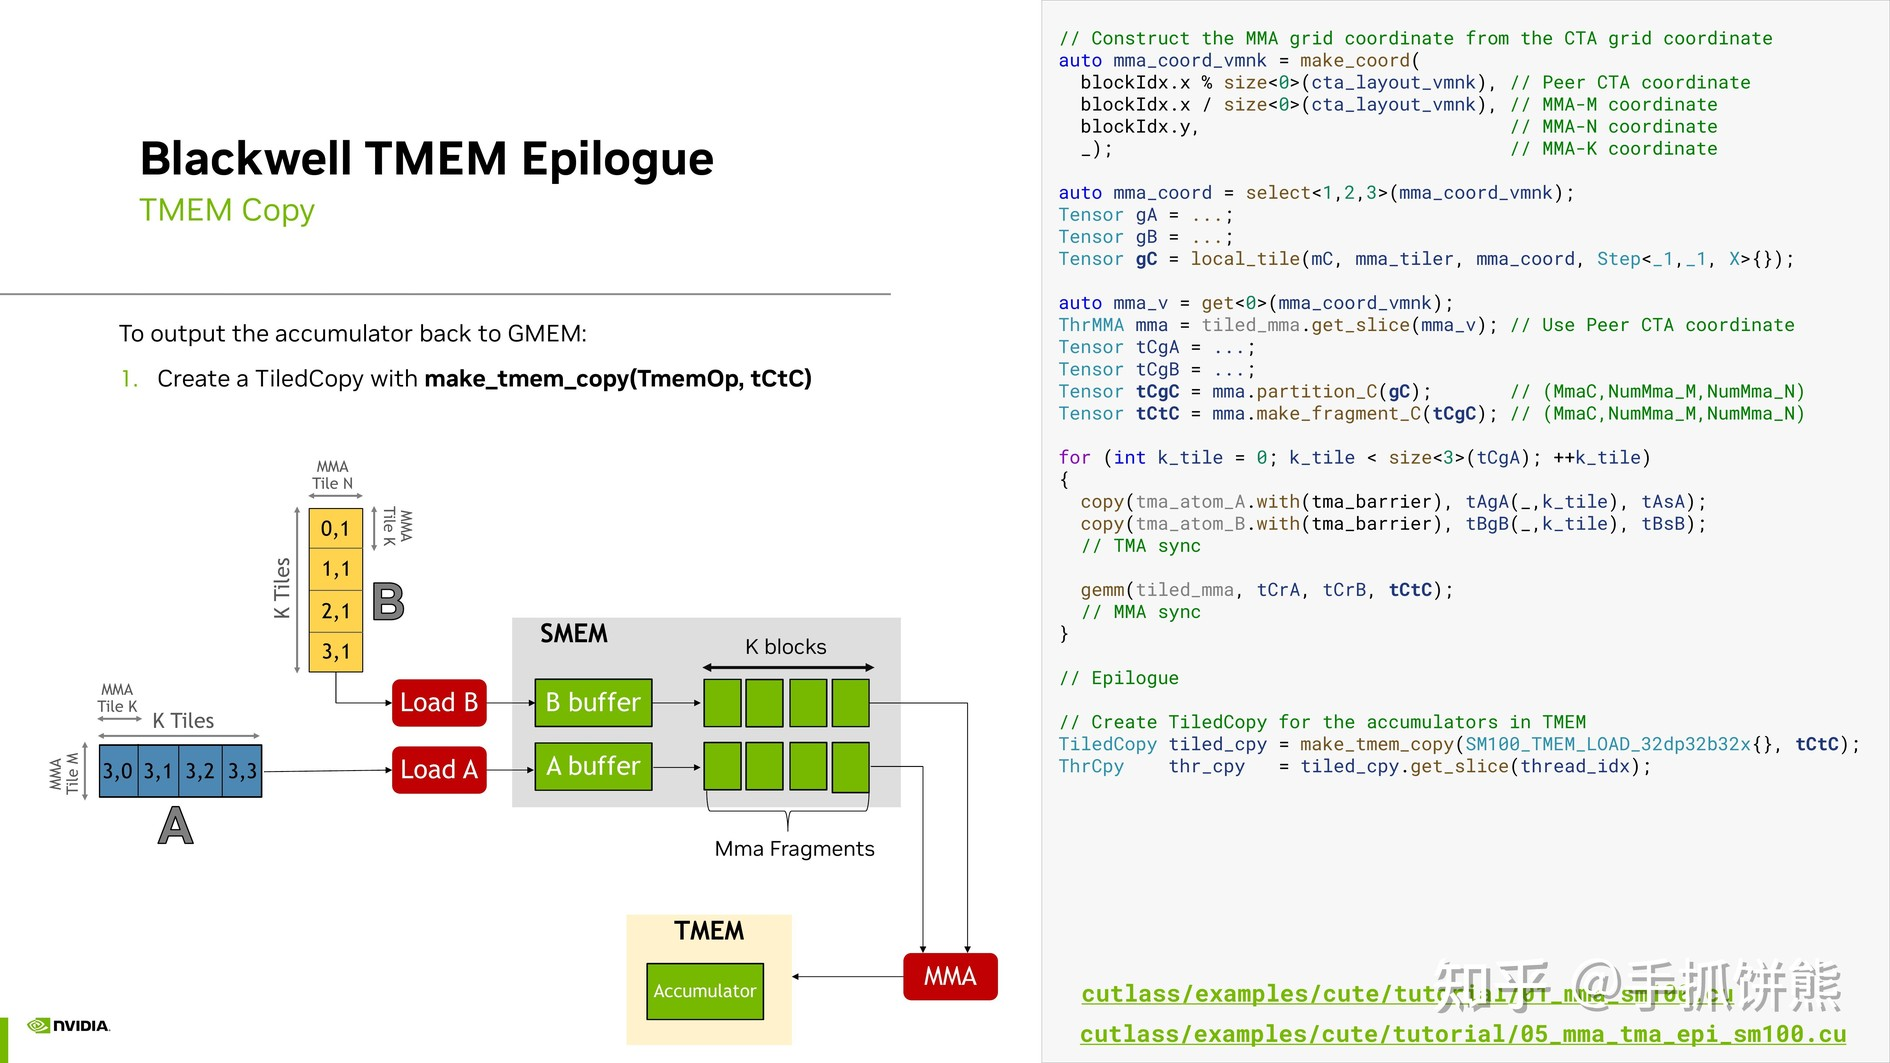
\includegraphics[width=0.9\textwidth]{figures/zhaoshangchun-01-tensor-core-programming/fig-46.jpg}
\end{figure}

GEMM 主循环结束后，累加结果完整地存放在 TMEM 中的 \texttt{t\allowbreak{}Ct\allowbreak{}C} 张量里。现在，Epilogue 的任务就是将这些结果写回全局内存。第 47 页介绍了这个过程的第一步：\textbf{为 TMEM 中的累加器创建一个 \texttt{Tiled\allowbreak{}Copy} 对象}。

\begin{lstlisting}[language=C++]
TiledCopy tiled_cpy = make_tmem_copy(SM100_TMEM_LOAD_32dp32b32x{}, tCtC);
\end{lstlisting}

上述代码是核心。这里的 \texttt{make\_\allowbreak{}tmem\_\allowbreak{}copy} 是一个工厂函数，它接收一个 \textbf{TMEM Copy Atom} (\texttt{S\allowbreak{}M\allowbreak{}1\allowbreak{}0\allowbreak{}0\allowbreak{}\_\allowbreak{}T\allowbreak{}M\allowbreak{}E\allowbreak{}M\allowbreak{}\_\allowbreak{}L\allowbreak{}O\allowbreak{}A\allowbreak{}D\allowbreak{}\_\allowbreak{}3\allowbreak{}2\allowbreak{}d\allowbreak{}p\allowbreak{}3\allowbreak{}2\allowbreak{}b\allowbreak{}3\allowbreak{}2\allowbreak{}x\allowbreak{}\{\allowbreak{}\}}) 和源张量 \texttt{t\allowbreak{}Ct\allowbreak{}C}，然后构造出一个 \texttt{Tiled\allowbreak{}Copy} 对象。这个 \texttt{Tiled\allowbreak{}Copy} 对象 \texttt{tiled\_\allowbreak{}cpy} 封装了从 TMEM 读取数据所需的全部信息，包括：

\begin{itemize}
\item \textbf{操作类型}：由 \texttt{SM100\_\allowbreak{}TMEM\_\allowbreak{}LOAD.\allowbreak{}.\allowbreak{}.\allowbreak{}} 定义，它代表了底层的 \texttt{tcgen05.\allowbreak{}load} PTX 指令变体。这个指令专门用于将数据从 TMEM 搬运到寄存器（RMEM）。\texttt{32dp32b32x} 可能表示每次操作处理的数据块大小、对齐方式等硬件细节。
\item \textbf{数据布局}：它从 \texttt{t\allowbreak{}Ct\allowbreak{}C} 继承了数据的逻辑布局，知道如何在 TMEM 中定位和寻址这些累加结果。
\item \textbf{分区策略}：\texttt{Tiled\allowbreak{}Copy} 知道如何将整个 \texttt{t\allowbreak{}Ct\allowbreak{}C} 的数据块在线程（Threads）之间进行划分。
\end{itemize}

随后，\texttt{T\allowbreak{}h\allowbreak{}r\allowbreak{}C\allowbreak{}p\allowbreak{}y\allowbreak{} \allowbreak{}t\allowbreak{}h\allowbreak{}r\allowbreak{}\_\allowbreak{}c\allowbreak{}p\allowbreak{}y\allowbreak{} \allowbreak{}=\allowbreak{} \allowbreak{}t\allowbreak{}i\allowbreak{}l\allowbreak{}e\allowbreak{}d\allowbreak{}\_\allowbreak{}c\allowbreak{}p\allowbreak{}y\allowbreak{}.\allowbreak{}g\allowbreak{}e\allowbreak{}t\allowbreak{}\_\allowbreak{}s\allowbreak{}l\allowbreak{}i\allowbreak{}c\allowbreak{}e\allowbreak{}(\allowbreak{}t\allowbreak{}h\allowbreak{}r\allowbreak{}e\allowbreak{}a\allowbreak{}d\allowbreak{}\_\allowbreak{}i\allowbreak{}d\allowbreak{}x\allowbreak{})\allowbreak{};} 为每个线程获取了它自己需要负责的那一小部分拷贝任务。这一步将集体层面的拷贝操作 (\texttt{Tiled\allowbreak{}Copy}) 分解为线程层面的具体操作 (\texttt{Thr\allowbreak{}Cpy})。之所以需要专门的 TMEM Copy Atom，是因为 TMEM 的访问方式与 SMEM 或 GMEM 不同，它要求特定的块布局和对齐，必须通过专用的 \texttt{tcgen05} 指令来操作。CUTLASS 将这些硬件约束抽象为 \texttt{Tiled\allowbreak{}Copy}，极大地简化了编程。

\textbf{第 48 页：TMEM Epilogue - Epilogue 第二步：分区与 RMEM 创建}

\begin{figure}[H]\centering
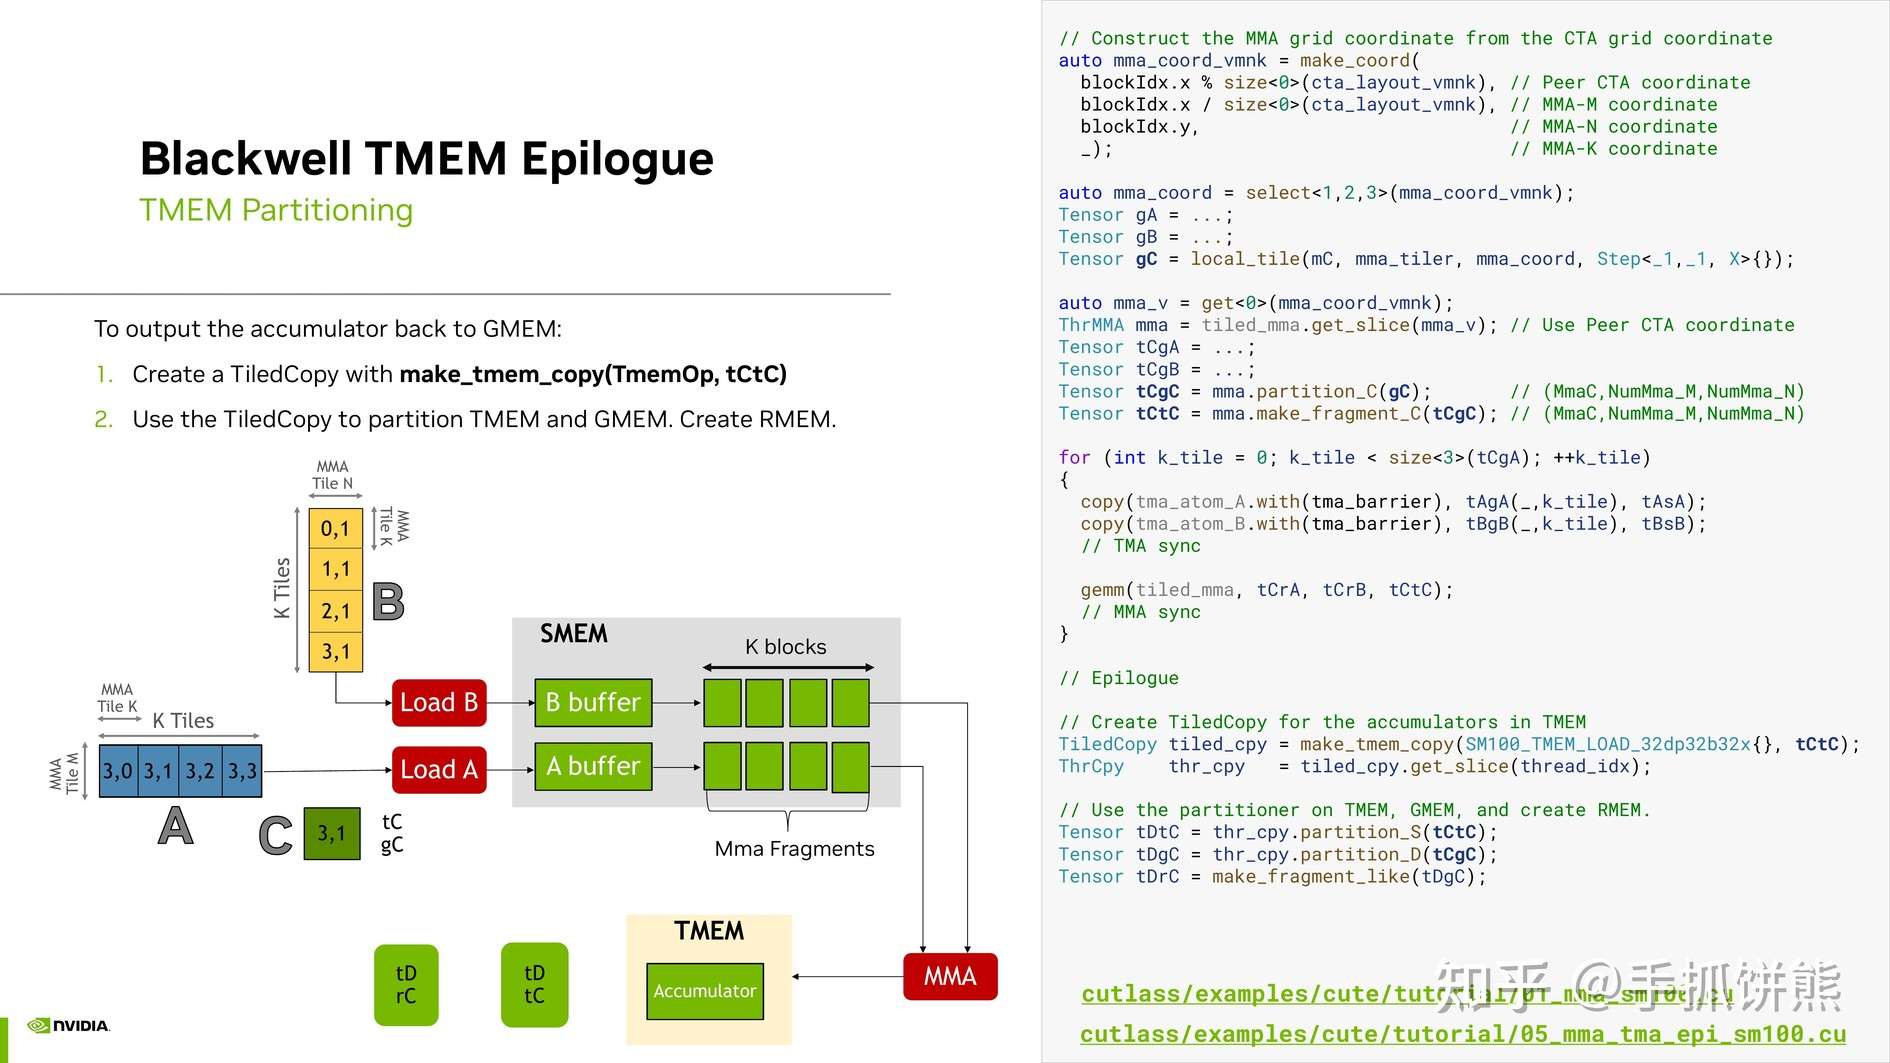
\includegraphics[width=0.9\textwidth]{figures/zhaoshangchun-01-tensor-core-programming/fig-47.jpg}
\end{figure}

创建了 \texttt{Tiled\allowbreak{}Copy} 之后，第 48 页展示了如何利用它来对不同层级的内存进行分区，并为最终的拷贝操作准备好“弹药”。

代码中连续调用了三次 \texttt{partition}：

\begin{enumerate}
\item \texttt{T\allowbreak{}e\allowbreak{}n\allowbreak{}s\allowbreak{}o\allowbreak{}r\allowbreak{} \allowbreak{}t\allowbreak{}D\allowbreak{}t\allowbreak{}C\allowbreak{} \allowbreak{}=\allowbreak{} \allowbreak{}t\allowbreak{}h\allowbreak{}r\allowbreak{}\_\allowbreak{}c\allowbreak{}p\allowbreak{}y\allowbreak{}.\allowbreak{}p\allowbreak{}a\allowbreak{}r\allowbreak{}t\allowbreak{}i\allowbreak{}t\allowbreak{}i\allowbreak{}o\allowbreak{}n\allowbreak{}\_\allowbreak{}S\allowbreak{}(\allowbreak{}t\allowbreak{}C\allowbreak{}t\allowbreak{}C\allowbreak{})\allowbreak{};}：\texttt{partition\_\allowbreak{}S} (S for Source) 使用 \texttt{thr\_\allowbreak{}cpy} 中定义的线程级分区策略，从 TMEM 张量 \texttt{t\allowbreak{}Ct\allowbreak{}C} 中为当前线程切分出它需要负责的\textbf{源数据分区 \texttt{t\allowbreak{}Dt\allowbreak{}C}}。\texttt{t\allowbreak{}Dt\allowbreak{}C} 描述了当前线程需要从 TMEM 读取哪一部分数据。
\item \texttt{T\allowbreak{}e\allowbreak{}n\allowbreak{}s\allowbreak{}o\allowbreak{}r\allowbreak{} \allowbreak{}t\allowbreak{}D\allowbreak{}g\allowbreak{}C\allowbreak{} \allowbreak{}=\allowbreak{} \allowbreak{}t\allowbreak{}h\allowbreak{}r\allowbreak{}\_\allowbreak{}c\allowbreak{}p\allowbreak{}y\allowbreak{}.\allowbreak{}p\allowbreak{}a\allowbreak{}r\allowbreak{}t\allowbreak{}i\allowbreak{}t\allowbreak{}i\allowbreak{}o\allowbreak{}n\allowbreak{}\_\allowbreak{}D\allowbreak{}(\allowbreak{}t\allowbreak{}C\allowbreak{}g\allowbreak{}C\allowbreak{})\allowbreak{};}：\texttt{partition\_\allowbreak{}D} (D for Destination) 同样使用 \texttt{thr\_\allowbreak{}cpy} 的策略，从之前定义的 CTA 本地全局内存视图 \texttt{t\allowbreak{}Cg\allowbreak{}C} 中，为当前线程切分出对应的\textbf{目标数据分区 \texttt{t\allowbreak{}Dg\allowbreak{}C}}。\texttt{t\allowbreak{}Dg\allowbreak{}C} 指向全局内存中的最终写入位置。
\item \texttt{T\allowbreak{}e\allowbreak{}n\allowbreak{}s\allowbreak{}o\allowbreak{}r\allowbreak{} \allowbreak{}t\allowbreak{}D\allowbreak{}r\allowbreak{}C\allowbreak{} \allowbreak{}=\allowbreak{} \allowbreak{}m\allowbreak{}a\allowbreak{}k\allowbreak{}e\allowbreak{}\_\allowbreak{}f\allowbreak{}r\allowbreak{}a\allowbreak{}g\allowbreak{}m\allowbreak{}e\allowbreak{}n\allowbreak{}t\allowbreak{}\_\allowbreak{}l\allowbreak{}i\allowbreak{}k\allowbreak{}e\allowbreak{}(\allowbreak{}t\allowbreak{}D\allowbreak{}g\allowbreak{}C\allowbreak{})\allowbreak{};}：这一步创建了一个\textbf{寄存器内存（RMEM）片段 \texttt{t\allowbreak{}Dr\allowbreak{}C}}。\texttt{make\_\allowbreak{}fragment\_\allowbreak{}like} 确保了 \texttt{t\allowbreak{}Dr\allowbreak{}C} 在形状和逻辑布局上与目标 \texttt{t\allowbreak{}Dg\allowbreak{}C} 完全匹配，但它的实际存储介质是线程的私有寄存器。\texttt{t\allowbreak{}Dr\allowbreak{}C} 将作为数据从 TMEM 到 GMEM 的\textbf{临时中转站}。
\end{enumerate}

这三步操作的核心思想是\textbf{“一次定义，多次使用”}。由 \texttt{Tiled\allowbreak{}Copy} 统一负责分区逻辑，保证了源（TMEM）、中转站（RMEM）和目的地（GMEM）三者之间的分区在逻辑上是完全一致的，避免了手动计算地址和偏移的复杂性和易错性。图示中的 \texttt{t\allowbreak{}Dt\allowbreak{}C}, \texttt{t\allowbreak{}Dr\allowbreak{}C}, \texttt{t\allowbreak{}Dg\allowbreak{}C} 正是这三个位于不同存储层级、但逻辑上对应的分区。

\textbf{第 49 页：TMEM Epilogue - Epilogue 第三步：TMEM→RMEM→GMEM}

\begin{figure}[H]\centering
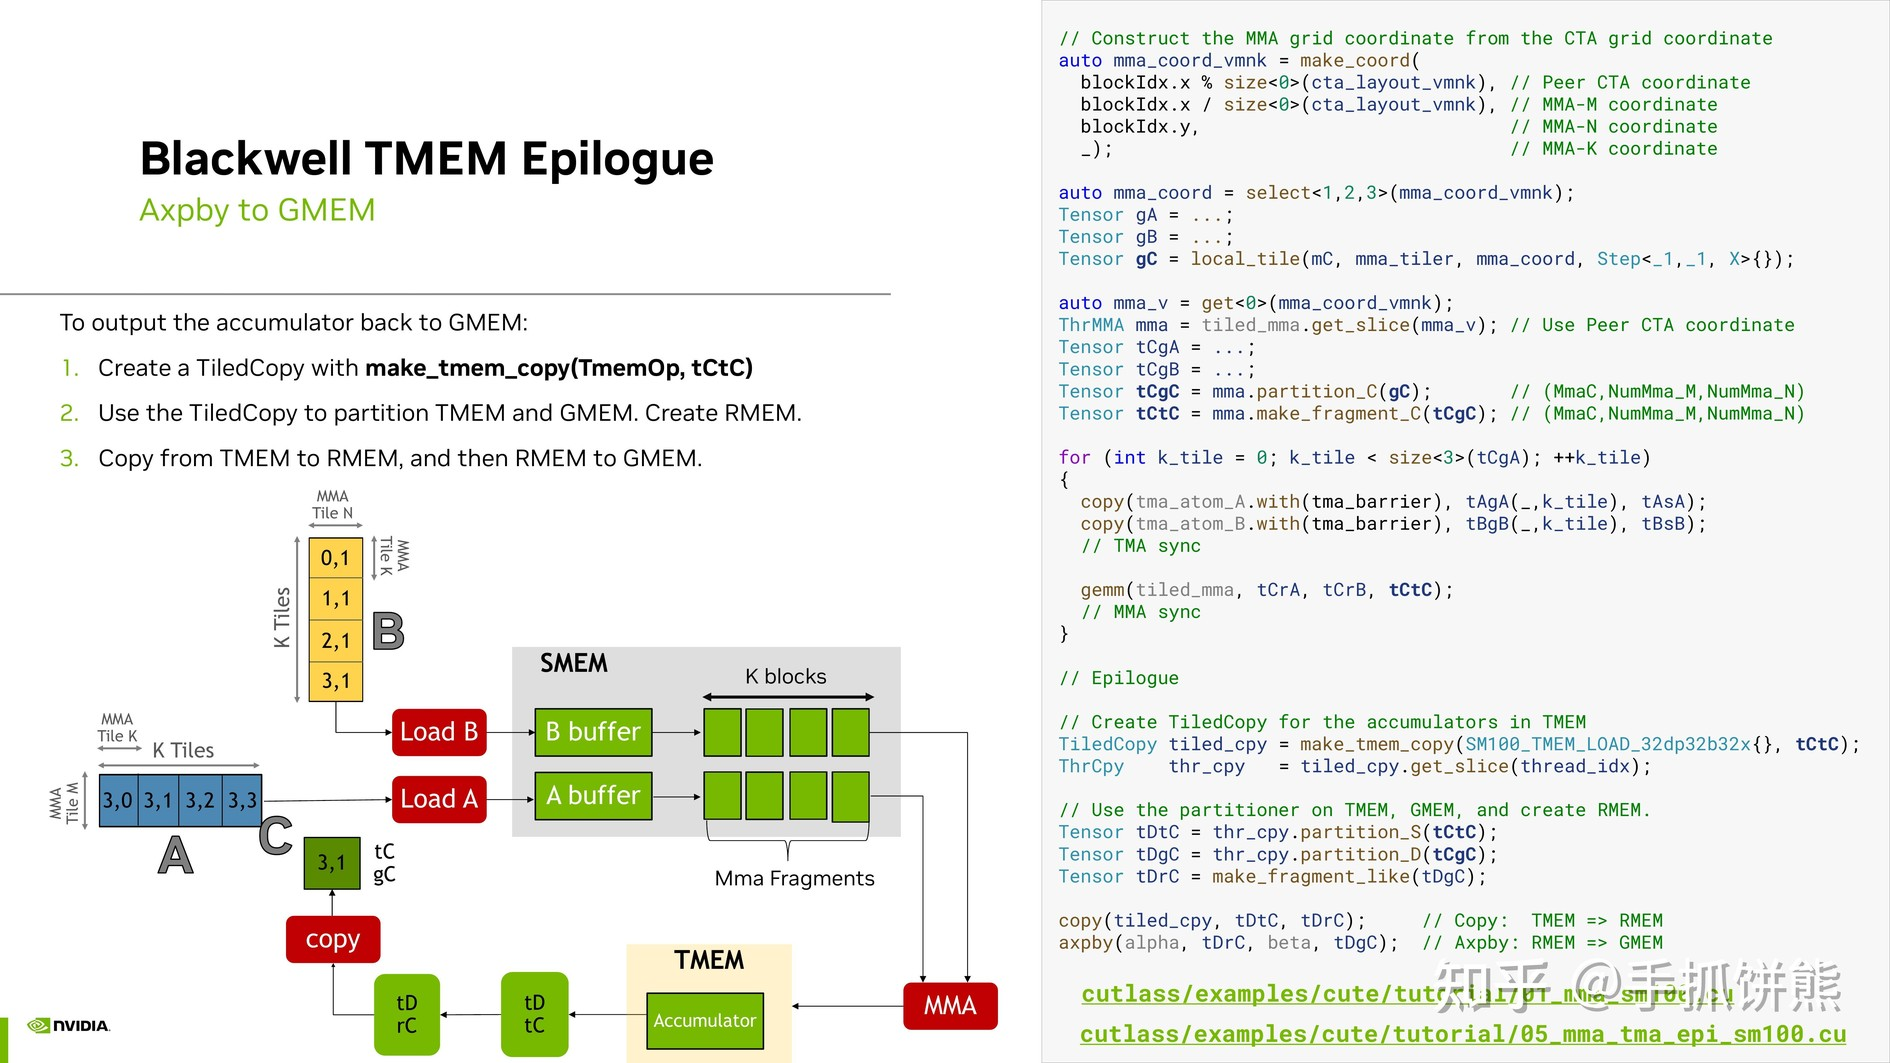
\includegraphics[width=0.9\textwidth]{figures/zhaoshangchun-01-tensor-core-programming/fig-48.jpg}
\end{figure}

万事俱备，第 49 页展示了 Epilogue 的最后一步：执行拷贝。这个过程被巧妙地分成了两个阶段。

第一阶段，\texttt{c\allowbreak{}o\allowbreak{}p\allowbreak{}y\allowbreak{}(\allowbreak{}t\allowbreak{}i\allowbreak{}l\allowbreak{}e\allowbreak{}d\allowbreak{}\_\allowbreak{}c\allowbreak{}p\allowbreak{}y\allowbreak{},\allowbreak{} \allowbreak{}t\allowbreak{}D\allowbreak{}t\allowbreak{}C\allowbreak{},\allowbreak{} \allowbreak{}t\allowbreak{}D\allowbreak{}r\allowbreak{}C\allowbreak{})\allowbreak{};} 执行了一次 \textbf{TMEM 到 RMEM 的拷贝}。

\begin{itemize}
\item \texttt{tiled\_\allowbreak{}cpy} 提供了拷贝操作的元数据和底层指令（即 \texttt{SM100\_\allowbreak{}TMEM\_\allowbreak{}LOAD}）。
\item \texttt{t\allowbreak{}Dt\allowbreak{}C} 是源，指向 TMEM 中的累加结果。
\item \texttt{t\allowbreak{}Dr\allowbreak{}C} 是目的地，是位于寄存器中的片段。执行后，每个线程负责的累加结果 Tile 就从 TMEM 被搬运到了各自的寄存器中。
\end{itemize}

第二阶段，\texttt{a\allowbreak{}x\allowbreak{}p\allowbreak{}b\allowbreak{}y\allowbreak{}(\allowbreak{}a\allowbreak{}l\allowbreak{}p\allowbreak{}h\allowbreak{}a\allowbreak{},\allowbreak{} \allowbreak{}t\allowbreak{}D\allowbreak{}r\allowbreak{}C\allowbreak{},\allowbreak{} \allowbreak{}b\allowbreak{}e\allowbreak{}t\allowbreak{}a\allowbreak{},\allowbreak{} \allowbreak{}t\allowbreak{}D\allowbreak{}g\allowbreak{}C\allowbreak{})\allowbreak{};} 完成了 \textbf{RMEM 到 GMEM 的最终写回}。

\begin{itemize}
\item \texttt{axpby} 是一个融合了线性变换和写回的函数，其语义是 \texttt{D = alpha * X + beta * D}。在这里，它代表 \texttt{G\allowbreak{}M\allowbreak{}E\allowbreak{}M\allowbreak{} \allowbreak{}=\allowbreak{} \allowbreak{}a\allowbreak{}l\allowbreak{}p\allowbreak{}h\allowbreak{}a\allowbreak{} \allowbreak{}*\allowbreak{} \allowbreak{}R\allowbreak{}M\allowbreak{}E\allowbreak{}M\allowbreak{} \allowbreak{}+\allowbreak{} \allowbreak{}b\allowbreak{}e\allowbreak{}t\allowbreak{}a\allowbreak{} \allowbreak{}*\allowbreak{} \allowbreak{}G\allowbreak{}M\allowbreak{}E\allowbreak{}M}。
\item \texttt{t\allowbreak{}Dr\allowbreak{}C} 是输入（来自 RMEM）。
\item \texttt{t\allowbreak{}Dg\allowbreak{}C} 既是输入（用于 \texttt{beta} 缩放）也是输出（最终写入的 GMEM 地址）。这个函数不仅将数据从 \texttt{t\allowbreak{}Dr\allowbreak{}C}（寄存器）写入 \texttt{t\allowbreak{}Dg\allowbreak{}C}（全局内存），还顺便完成了 \texttt{C\allowbreak{} \allowbreak{}=\allowbreak{} \allowbreak{}a\allowbreak{}l\allowbreak{}p\allowbreak{}h\allowbreak{}a\allowbreak{} \allowbreak{}*\allowbreak{} \allowbreak{}A\allowbreak{} \allowbreak{}*\allowbreak{} \allowbreak{}B\allowbreak{} \allowbreak{}+\allowbreak{} \allowbreak{}b\allowbreak{}e\allowbreak{}t\allowbreak{}a\allowbreak{} \allowbreak{}*\allowbreak{} \allowbreak{}C} 这个标准 GEMM 公式中的 \texttt{alpha} 和 \texttt{beta} 缩放与偏移操作。
\end{itemize}

\textbf{为什么分成两步？} 这种 \textbf{TMEM → RMEM → GMEM} 的两阶段 Epilogue 设计是 CUTLASS 优化的核心思想之一。将 TMEM load 和 GMEM store 分离开，使得：

\begin{enumerate}
\item \textbf{优化内存访问}：可以在 \texttt{copy} 和 \texttt{axpby} 之间插入 \texttt{\_\allowbreak{}\_\allowbreak{}syncthreads()} 或其他同步原语，确保所有线程都完成了从 TMEM 的读取，然后再一起写入 GMEM，这有助于优化缓存行为和写合并。
\item \textbf{增加融合机会}：在 RMEM 中，数据位于寄存器，可以进行非常灵活和高效的 SIMT 计算。在 \texttt{copy} 和 \texttt{axpby} 之间，可以插入任意复杂的元素级操作（如激活函数、量化/\allowbreak{}反量化等），而不会影响访存流水线。这种设计将数据移动与计算解耦，是 CUTLASS 实现高性能、可组合 Epilogue 的关键。
\end{enumerate}

\section{\textbf{四、使用 CUTLASS 驾驭 Blackwell 新特性}}

本章将展示 CUTLASS 4.0 如何将第三章中复杂的 Cu\allowbreak{}Te 编程范式，封装成高度模块化、易于组合的“Collective”组件，让开发者能够以声明式的方式，快速构建出针对 Blackwell 优化的、生产力级别的核函数。

\subsection{\textbf{CUTLASS 的声明式编程模型}}

本小节将介绍 CUTLASS 4.0 的核心设计理念——Collective 编程模型，并展示如何通过简单的“填表”方式，构建一个完整的、针对 Blackwell 优化的 GEMM 内核。

\textbf{第 50 页：章节目录过渡部分}

\begin{figure}[H]\centering
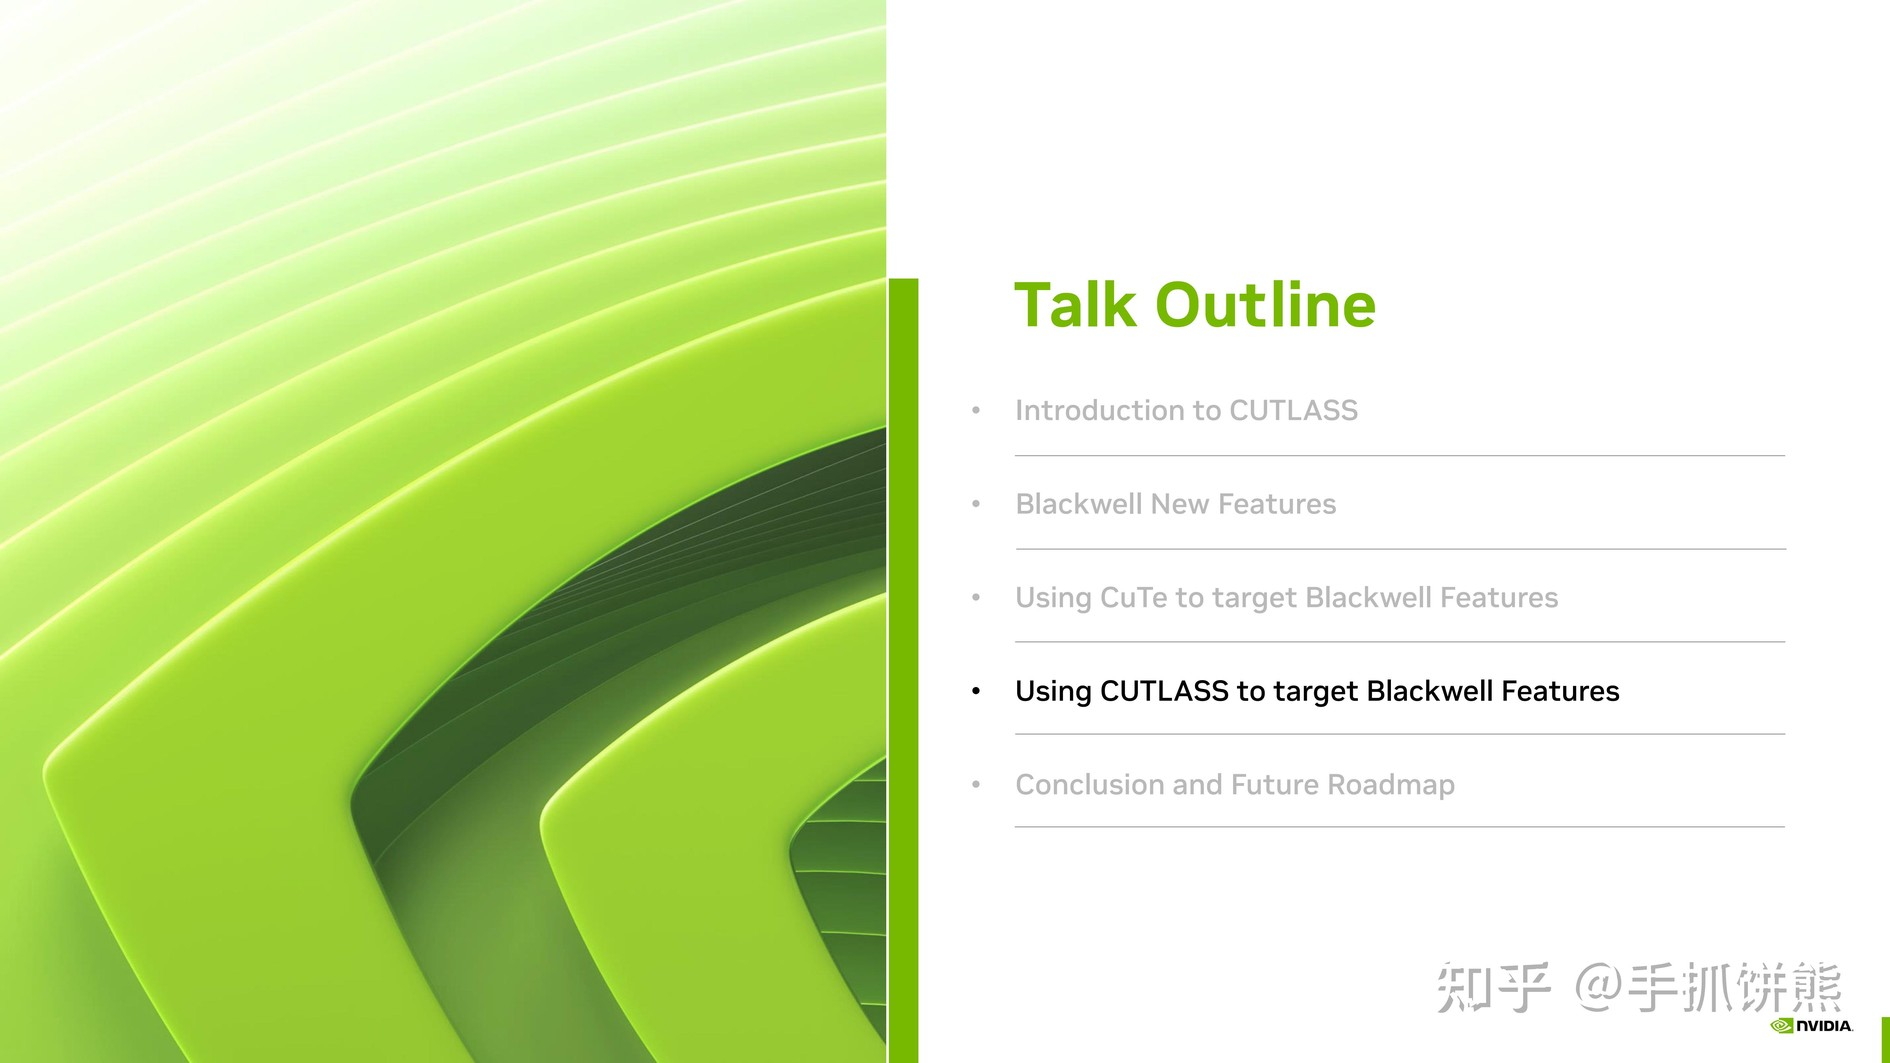
\includegraphics[width=0.9\textwidth]{figures/zhaoshangchun-01-tensor-core-programming/fig-49.jpg}
\end{figure}

从本页开始 Using CUTLASS to target Blackwell Features。前面的章节，我们学习了用 Cu\allowbreak{}Te 来使用Blackwell，从这一章开始，我们将切换到“框架开发者”的视角，看看 CUTLASS 是如何将这些底层复杂性封装起来，提供更友好、更高效的编程接口的。

这个过渡至关重要，它揭示了 NVIDIA 软件栈的分层设计哲学：Cu\allowbreak{}Te 负责提供表达能力和对硬件的终极控制，而 CUTLASS 则在此基础上负责提供生产力和易用性。

\textbf{第 51 页：CUTLASS 面临的组合爆炸问题}

\begin{figure}[H]\centering
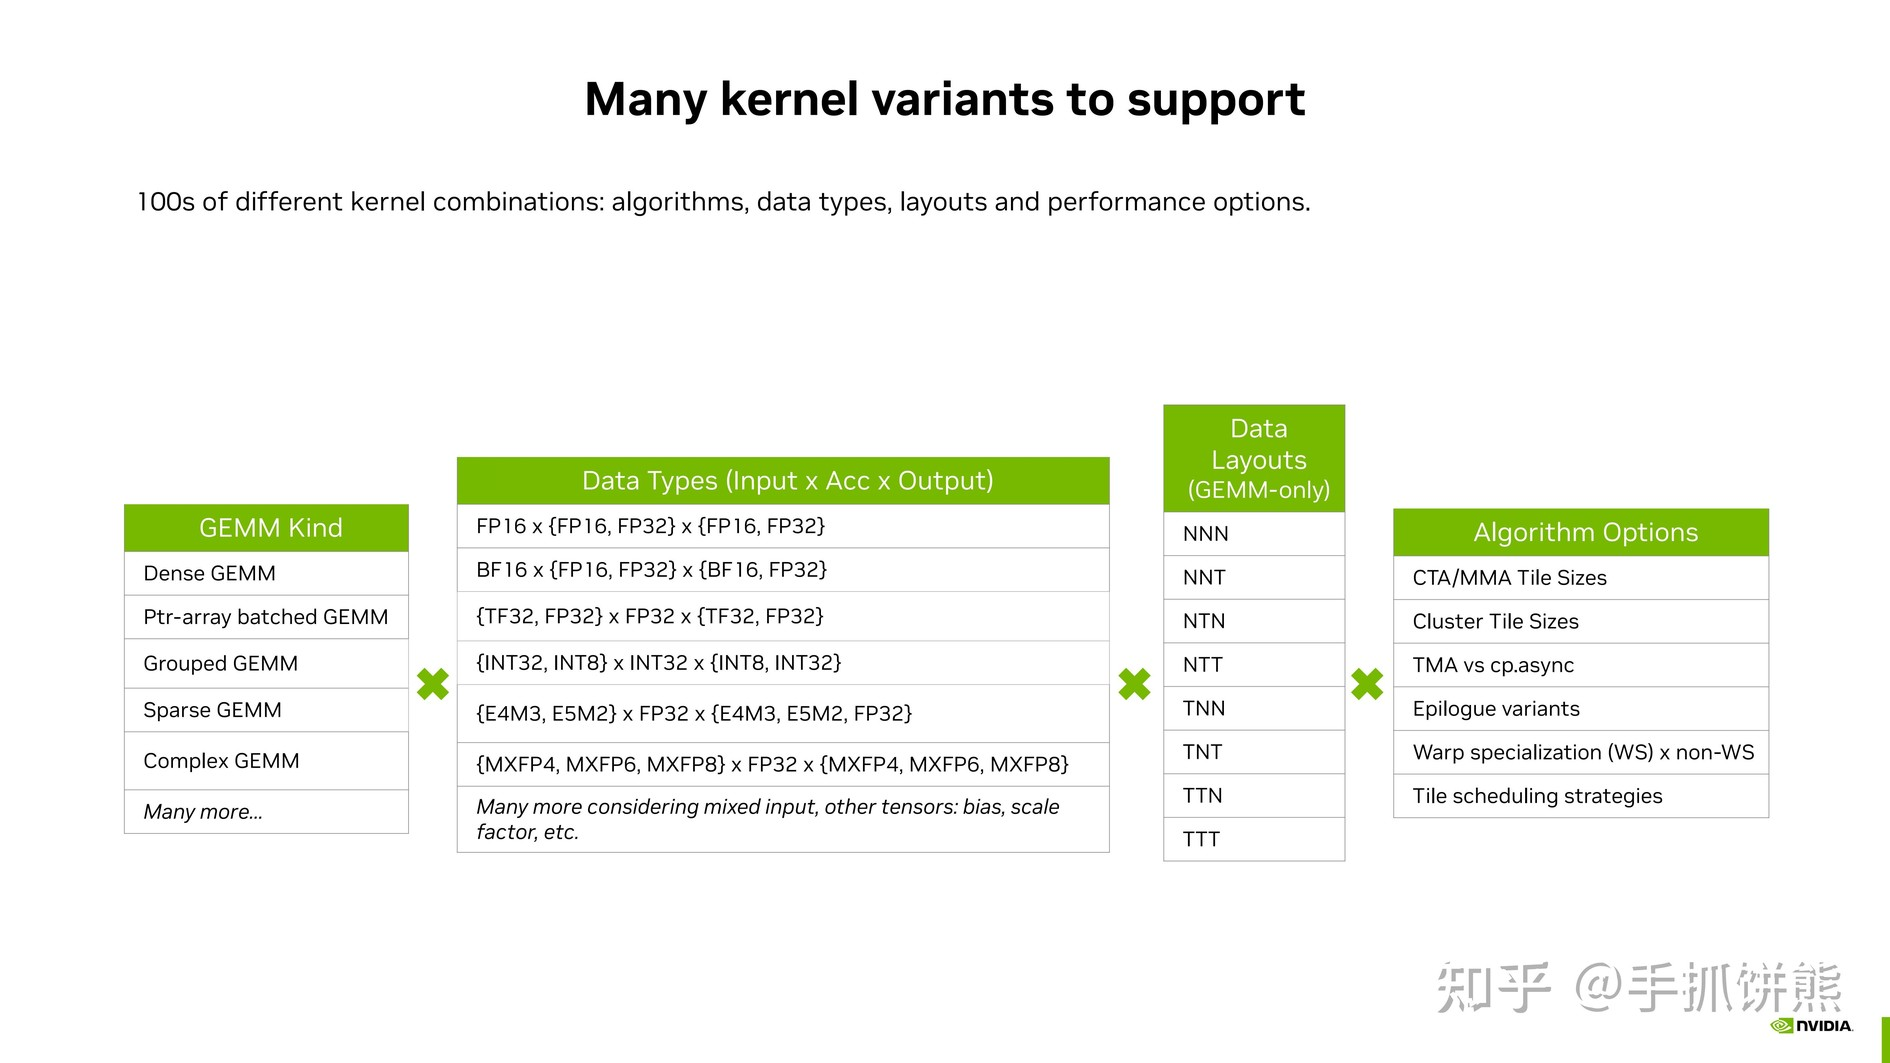
\includegraphics[width=0.9\textwidth]{figures/zhaoshangchun-01-tensor-core-programming/fig-50.jpg}
\end{figure}

这一页直观地展示了 CUTLASS 需要解决的核心挑战——\textbf{组合爆炸}。一个看似简单的 GEMM 操作，背后却隐藏着海量的变化维度：GEMM 类型、数据类型、数据布局、算法选项等等。将这些维度排列组合，会产生成百上千种不同的核函数变体。如果为每一种变体都手写一个内核，将是不可想象的维护噩梦。

CUTLASS 的核心价值就在于，通过\textbf{模板元编程和高度抽象}，提供了一套能够灵活生成所有这些变体的通用框架。它不是提供一堆固定的核函数，而是提供一套生成核函数的“工厂”。理解了这一点，就能明白为什么 CUTLASS 的代码看起来如此复杂，因为它正在解决一个本质上就非常复杂的问题。

\textbf{第 52 页：CUTLASS 3.x 的概念层级}

\begin{figure}[H]\centering
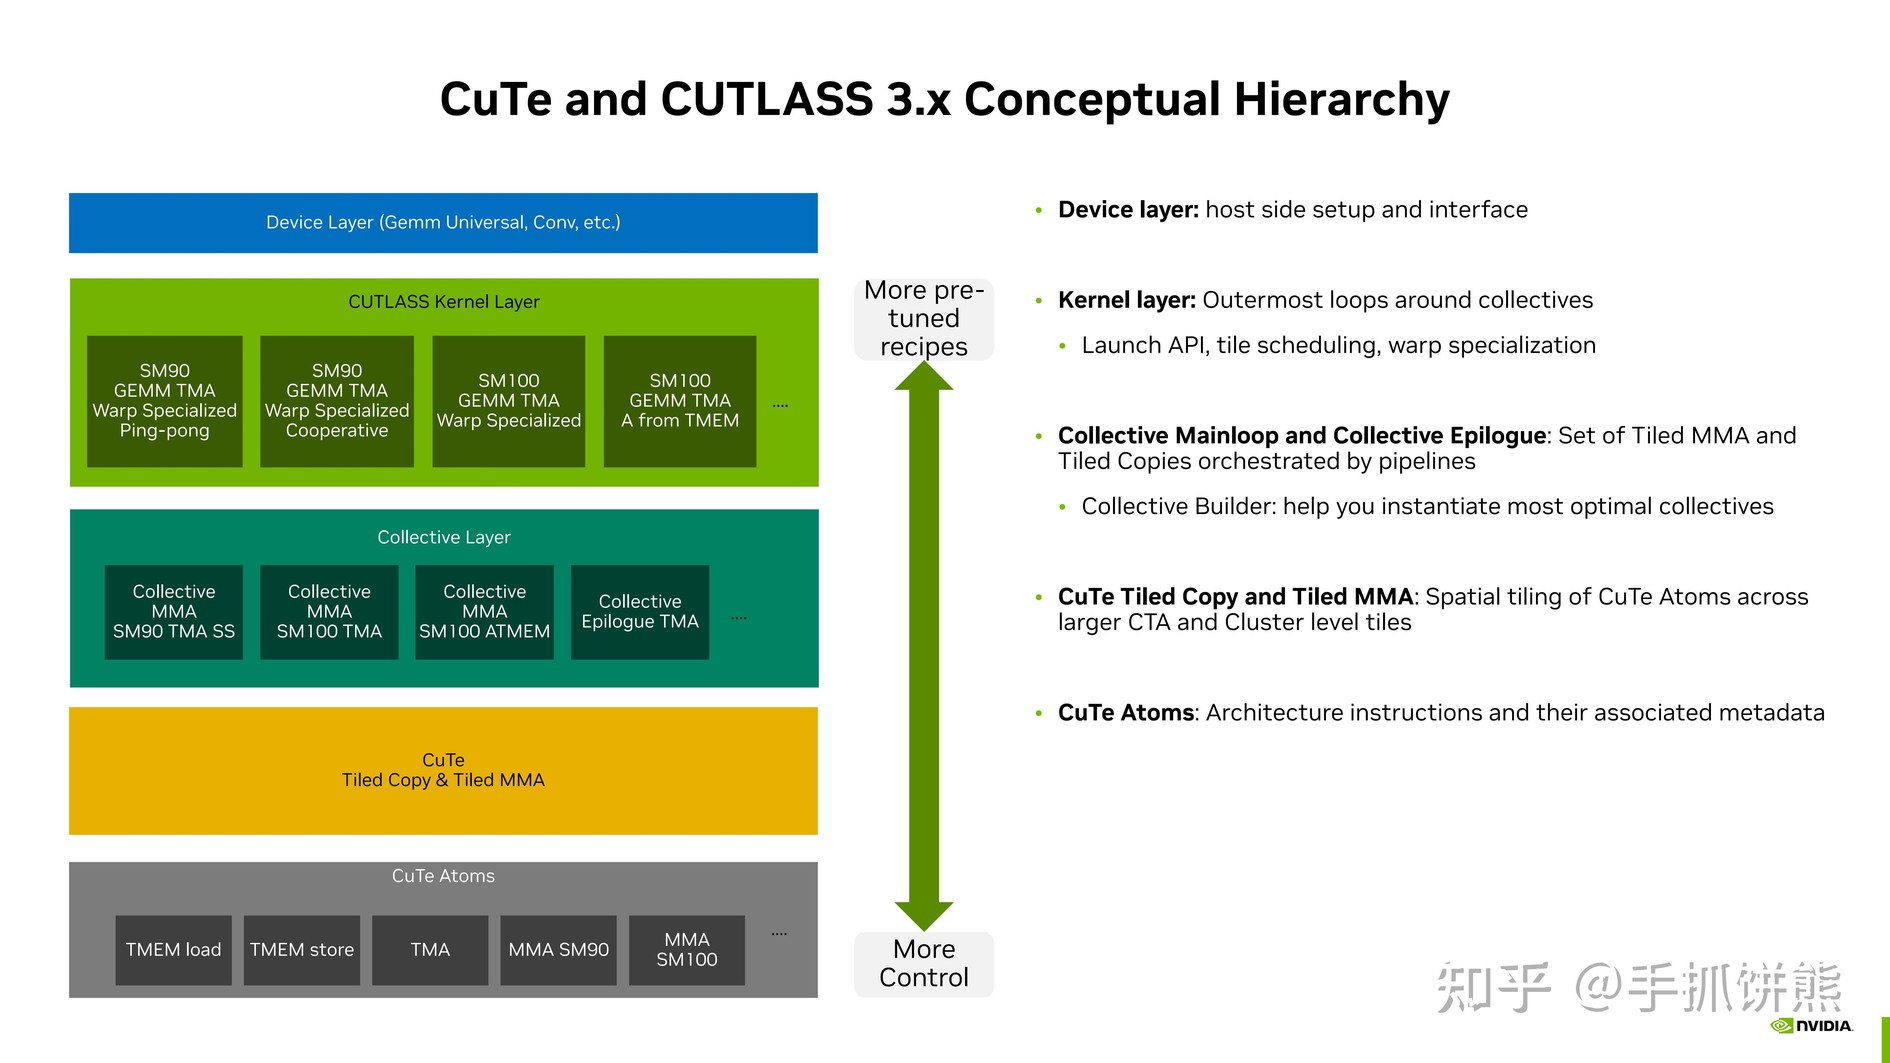
\includegraphics[width=0.9\textwidth]{figures/zhaoshangchun-01-tensor-core-programming/fig-51.jpg}
\end{figure}

这一页清晰地描绘了 CUTLASS 3.x（以及 4.0）的软件栈层次结构。自底向上，从最底层的硬件指令封装 \texttt{Cu\allowbreak{}Te Atoms}，到中间的 \texttt{C\allowbreak{}u\allowbreak{}T\allowbreak{}e\allowbreak{} \allowbreak{}T\allowbreak{}i\allowbreak{}l\allowbreak{}e\allowbreak{}d\allowbreak{} \allowbreak{}C\allowbreak{}o\allowbreak{}p\allowbreak{}y\allowbreak{} \allowbreak{}\&\allowbreak{} \allowbreak{}T\allowbreak{}i\allowbreak{}l\allowbreak{}e\allowbreak{}d\allowbreak{} \allowbreak{}M\allowbreak{}M\allowbreak{}A}，再到 \textbf{CUTLASS 4.0 的核心抽象层：Collective Layer}。\texttt{Collective Mainloop} 负责数据加载和 MMA 计算的流水线，\texttt{Collective Epilogue} 负责结果的写回和融合操作。将这两者组合，再配上一个调度策略，就构成了一个完整的 \texttt{Kernel}。

这个分层架构提供了不同层次的控制力。硬件专家可以在 Cu\allowbreak{}Te Atoms 层进行极致创新；算子开发者可以在 Collective 层自由组合预置的最优实践；而应用开发者则可以直接使用 Device 层的通用 GEMM 内核。对于大多数人来说，只需要在 \texttt{Collective Layer} 和 \texttt{Kernel Layer} 进行“声明式编程”，就能获得顶级的性能，这极大地提升了开发效率。

\subsection{CUTLASS 内核示例}

本小节从 53-57 页，讲解了CUTLASS如何实现一个kernel，整体非常的简洁。

\textbf{第 53 页：CUTLASS Kernel Example}

\begin{figure}[H]\centering
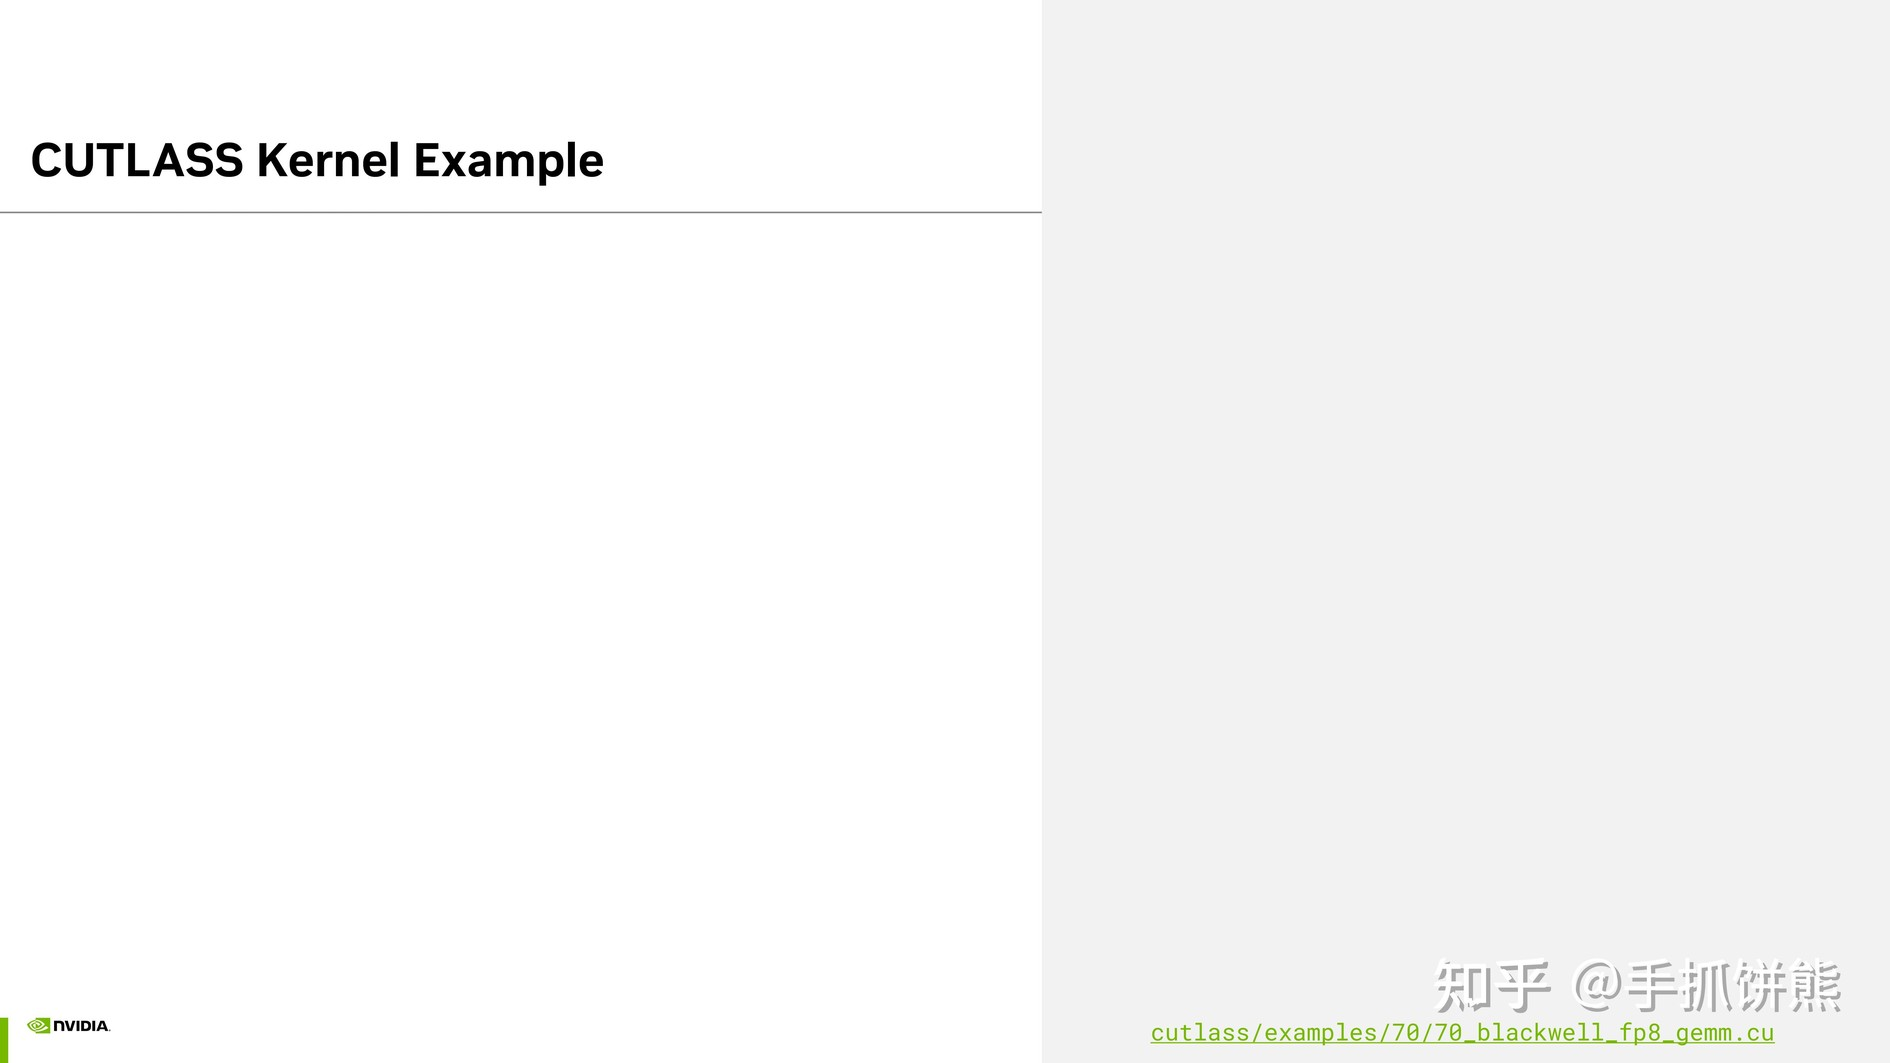
\includegraphics[width=0.9\textwidth]{figures/zhaoshangchun-01-tensor-core-programming/fig-52.jpg}
\end{figure}

这一页非常简洁，只给出了一个标题和一个文件路径\texttt{c\allowbreak{}u\allowbreak{}t\allowbreak{}l\allowbreak{}a\allowbreak{}s\allowbreak{}s\allowbreak{}/\allowbreak{}e\allowbreak{}x\allowbreak{}a\allowbreak{}m\allowbreak{}p\allowbreak{}l\allowbreak{}e\allowbreak{}s\allowbreak{}/\allowbreak{}7\allowbreak{}0\allowbreak{}\_\allowbreak{}b\allowbreak{}l\allowbreak{}a\allowbreak{}c\allowbreak{}k\allowbreak{}w\allowbreak{}e\allowbreak{}l\allowbreak{}l\allowbreak{}\_\allowbreak{}f\allowbreak{}p\allowbreak{}8\allowbreak{}\_\allowbreak{}g\allowbreak{}e\allowbreak{}m\allowbreak{}m\allowbreak{}.\allowbreak{}c\allowbreak{}u}。接下来我们将通过一个具体的例子，来展示 CUTLASS 的威力。

从文件名我们可以解读出关键信息：这个例子是关于在 \textbf{Blackwell} 架构上，使用 \textbf{FP8} 这种新的低比特数据类型，来实现 \textbf{GEMM} 运算。这几乎涵盖了 Blackwell 在计算方面所有的新特性。通过这个例子，我们将亲眼见证 CUTLASS 是如何将前面讨论的所有复杂概念（2-SM-MMA、TMEM、MXFP8、动态调度等）无缝地整合在一起的。

\textbf{第 54页：一个完整的 CUTLASS 内核示例，cutlass::\allowbreak{}gemm::\allowbreak{}collective::\allowbreak{}Collective\allowbreak{}Builder}

\begin{figure}[H]\centering
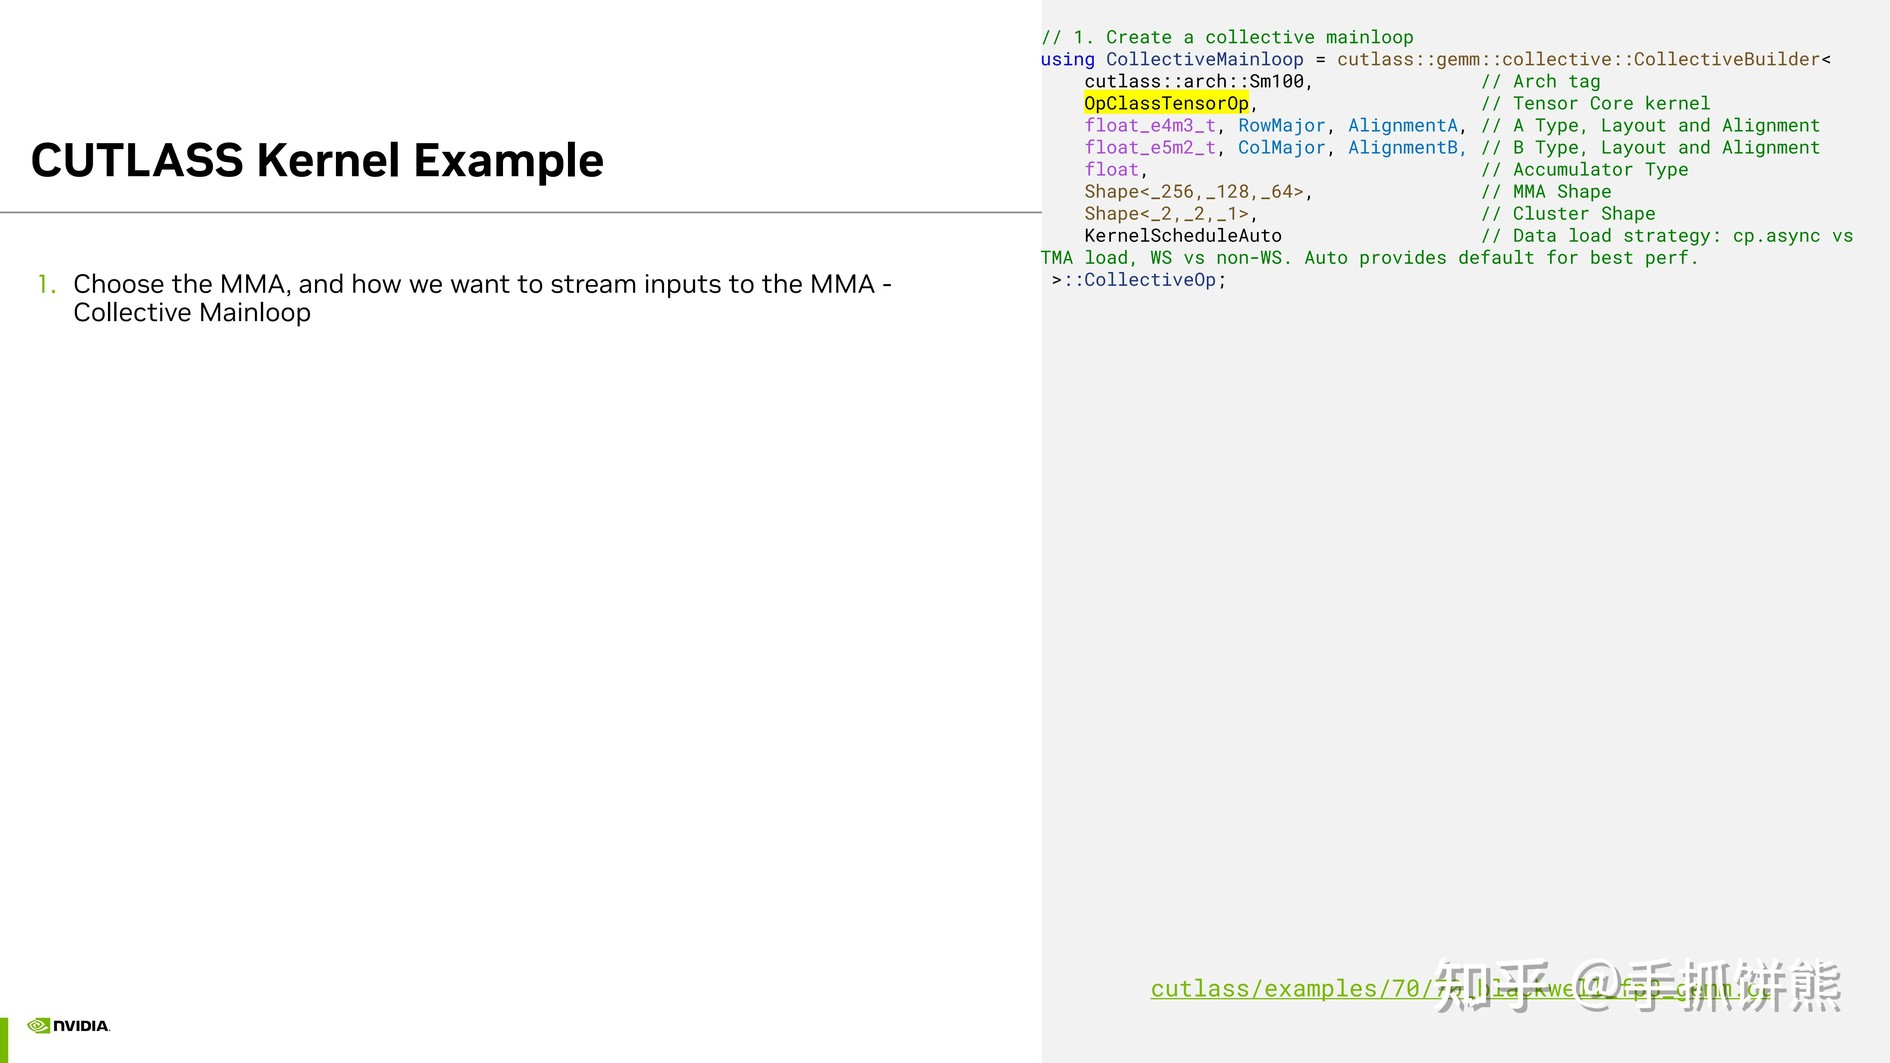
\includegraphics[width=0.9\textwidth]{figures/zhaoshangchun-01-tensor-core-programming/fig-53.jpg}
\end{figure}

\begin{itemize}
\item 使用 \texttt{c\allowbreak{}u\allowbreak{}t\allowbreak{}l\allowbreak{}a\allowbreak{}s\allowbreak{}s\allowbreak{}:\allowbreak{}:\allowbreak{}g\allowbreak{}e\allowbreak{}m\allowbreak{}m\allowbreak{}:\allowbreak{}:\allowbreak{}c\allowbreak{}o\allowbreak{}l\allowbreak{}l\allowbreak{}e\allowbreak{}c\allowbreak{}t\allowbreak{}i\allowbreak{}v\allowbreak{}e\allowbreak{}:\allowbreak{}:\allowbreak{}C\allowbreak{}o\allowbreak{}l\allowbreak{}l\allowbreak{}e\allowbreak{}c\allowbreak{}t\allowbreak{}i\allowbreak{}v\allowbreak{}e\allowbreak{}B\allowbreak{}u\allowbreak{}i\allowbreak{}l\allowbreak{}d\allowbreak{}e\allowbreak{}r}。
\item 指定模板参数：
\item \texttt{cutlass::\allowbreak{}arch::\allowbreak{}Sm100}：架构 tag，明确表示为 Blackwell。
\item \texttt{float\_\allowbreak{}e4m3\_\allowbreak{}t}, \texttt{float\_\allowbreak{}e5m2\_\allowbreak{}t}：输入 A 和 B 的数据类型（FP8 的两种变体）。
\item \texttt{Shape<\_\allowbreak{}256,\allowbreak{}\_\allowbreak{}128,\allowbreak{}\_\allowbreak{}64>}：\textbf{MMA Shape} (M, N, K)。
\item \texttt{Shape<\_\allowbreak{}2,\allowbreak{}\_\allowbreak{}2,\allowbreak{}\_\allowbreak{}1>}：\textbf{Cluster Shape}。
\item \texttt{Kernel\allowbreak{}Schedule\allowbreak{}Auto}：让 CUTLASS 自动选择数据加载策略（TMA, WS 等）。
\end{itemize}

\textbf{第 55 页：一个完整的 CUTLASS 内核示例，创建 \texttt{Collective\allowbreak{}Epilogue}}

\begin{figure}[H]\centering
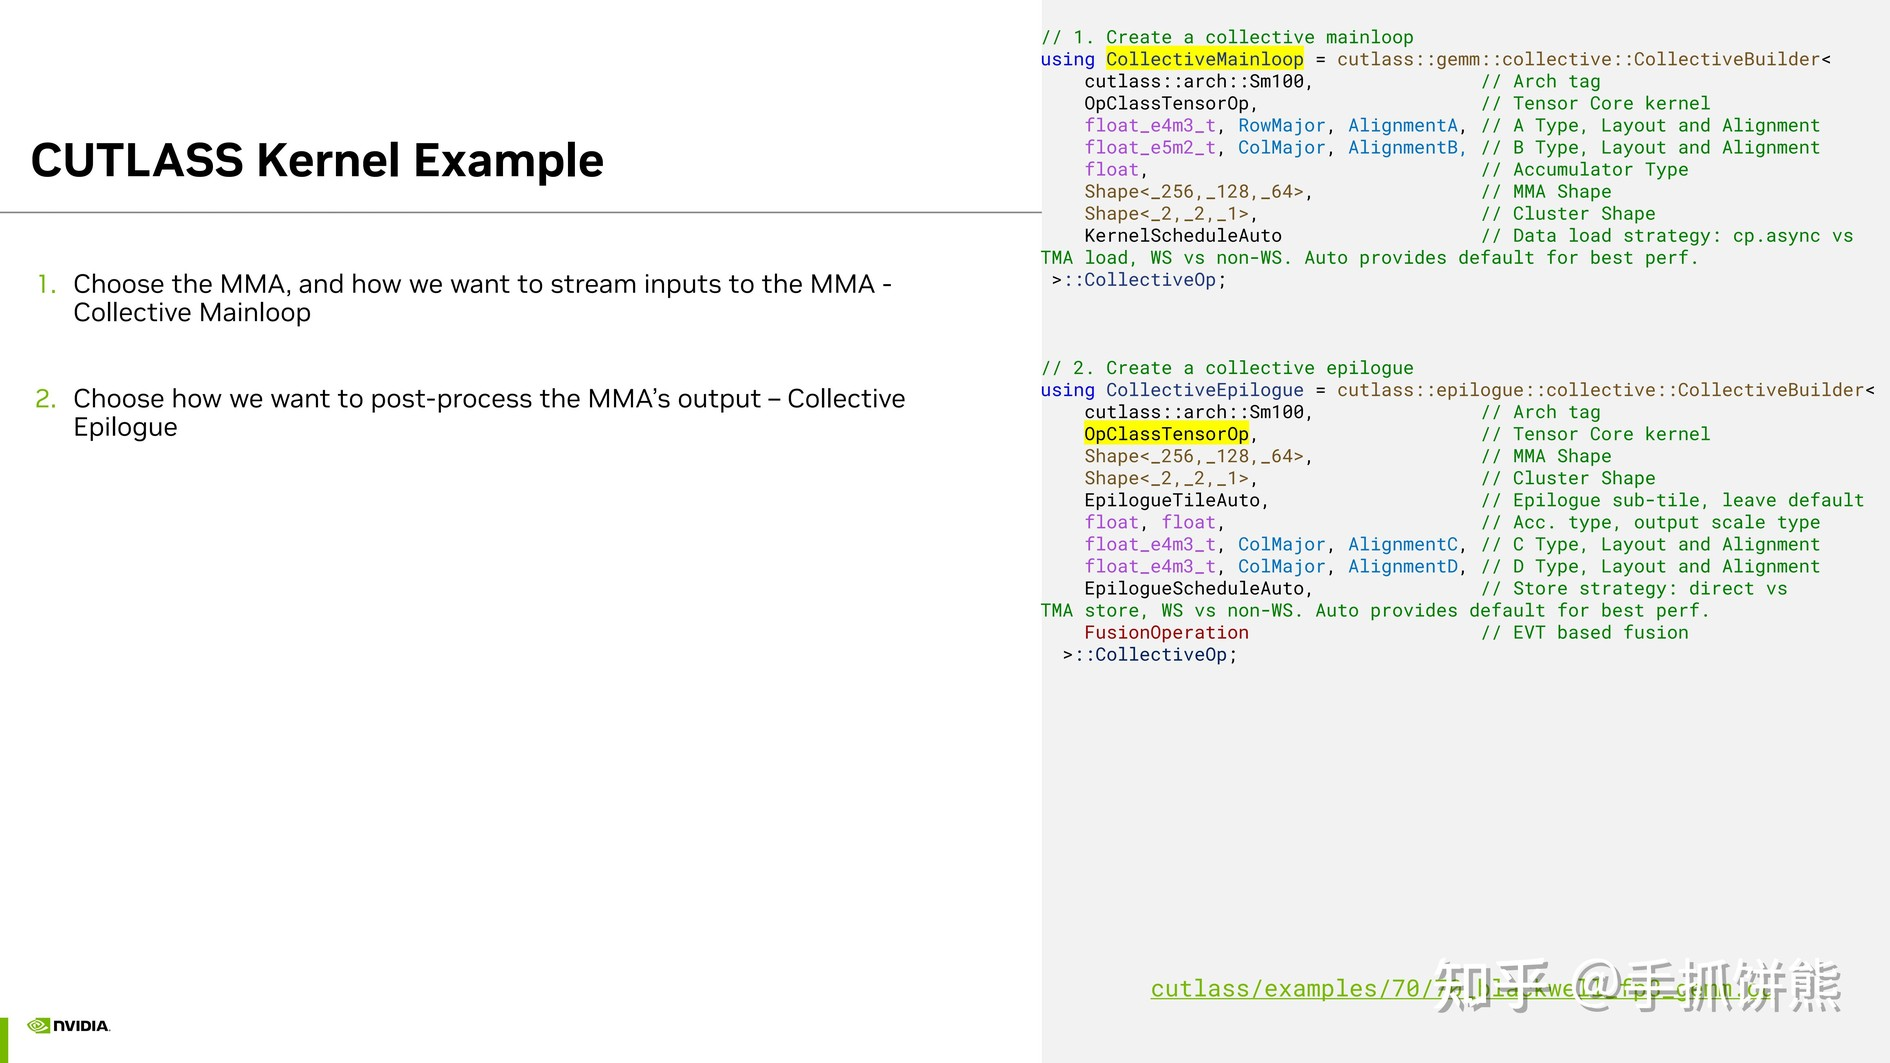
\includegraphics[width=0.9\textwidth]{figures/zhaoshangchun-01-tensor-core-programming/fig-54.jpg}
\end{figure}

\begin{itemize}
\item 同样使用 \texttt{c\allowbreak{}u\allowbreak{}t\allowbreak{}l\allowbreak{}a\allowbreak{}s\allowbreak{}s\allowbreak{}:\allowbreak{}:\allowbreak{}e\allowbreak{}p\allowbreak{}i\allowbreak{}l\allowbreak{}o\allowbreak{}g\allowbreak{}u\allowbreak{}e\allowbreak{}:\allowbreak{}:\allowbreak{}c\allowbreak{}o\allowbreak{}l\allowbreak{}l\allowbreak{}e\allowbreak{}c\allowbreak{}t\allowbreak{}i\allowbreak{}v\allowbreak{}e\allowbreak{}:\allowbreak{}:\allowbreak{}C\allowbreak{}o\allowbreak{}l\allowbreak{}l\allowbreak{}e\allowbreak{}c\allowbreak{}t\allowbreak{}i\allowbreak{}v\allowbreak{}e\allowbreak{}B\allowbreak{}u\allowbreak{}i\allowbreak{}l\allowbreak{}d\allowbreak{}e\allowbreak{}r}。
\item 传入与 Mainloop 匹配的架构、MMA Shape 和 Cluster Shape。
\item 指定输出 D 和 C 的类型、布局。
\item \texttt{Epilogue\allowbreak{}Schedule\allowbreak{}Auto}：让 CUTLASS 自动选择存储策略。
\item \texttt{Fusion\allowbreak{}Operation}：用于注入自定义 Epilogue 融合逻辑的钩子。
\end{itemize}

\textbf{第 56 页：一个完整的 CUTLASS 内核示例，组合成 Kernel}

\begin{figure}[H]\centering
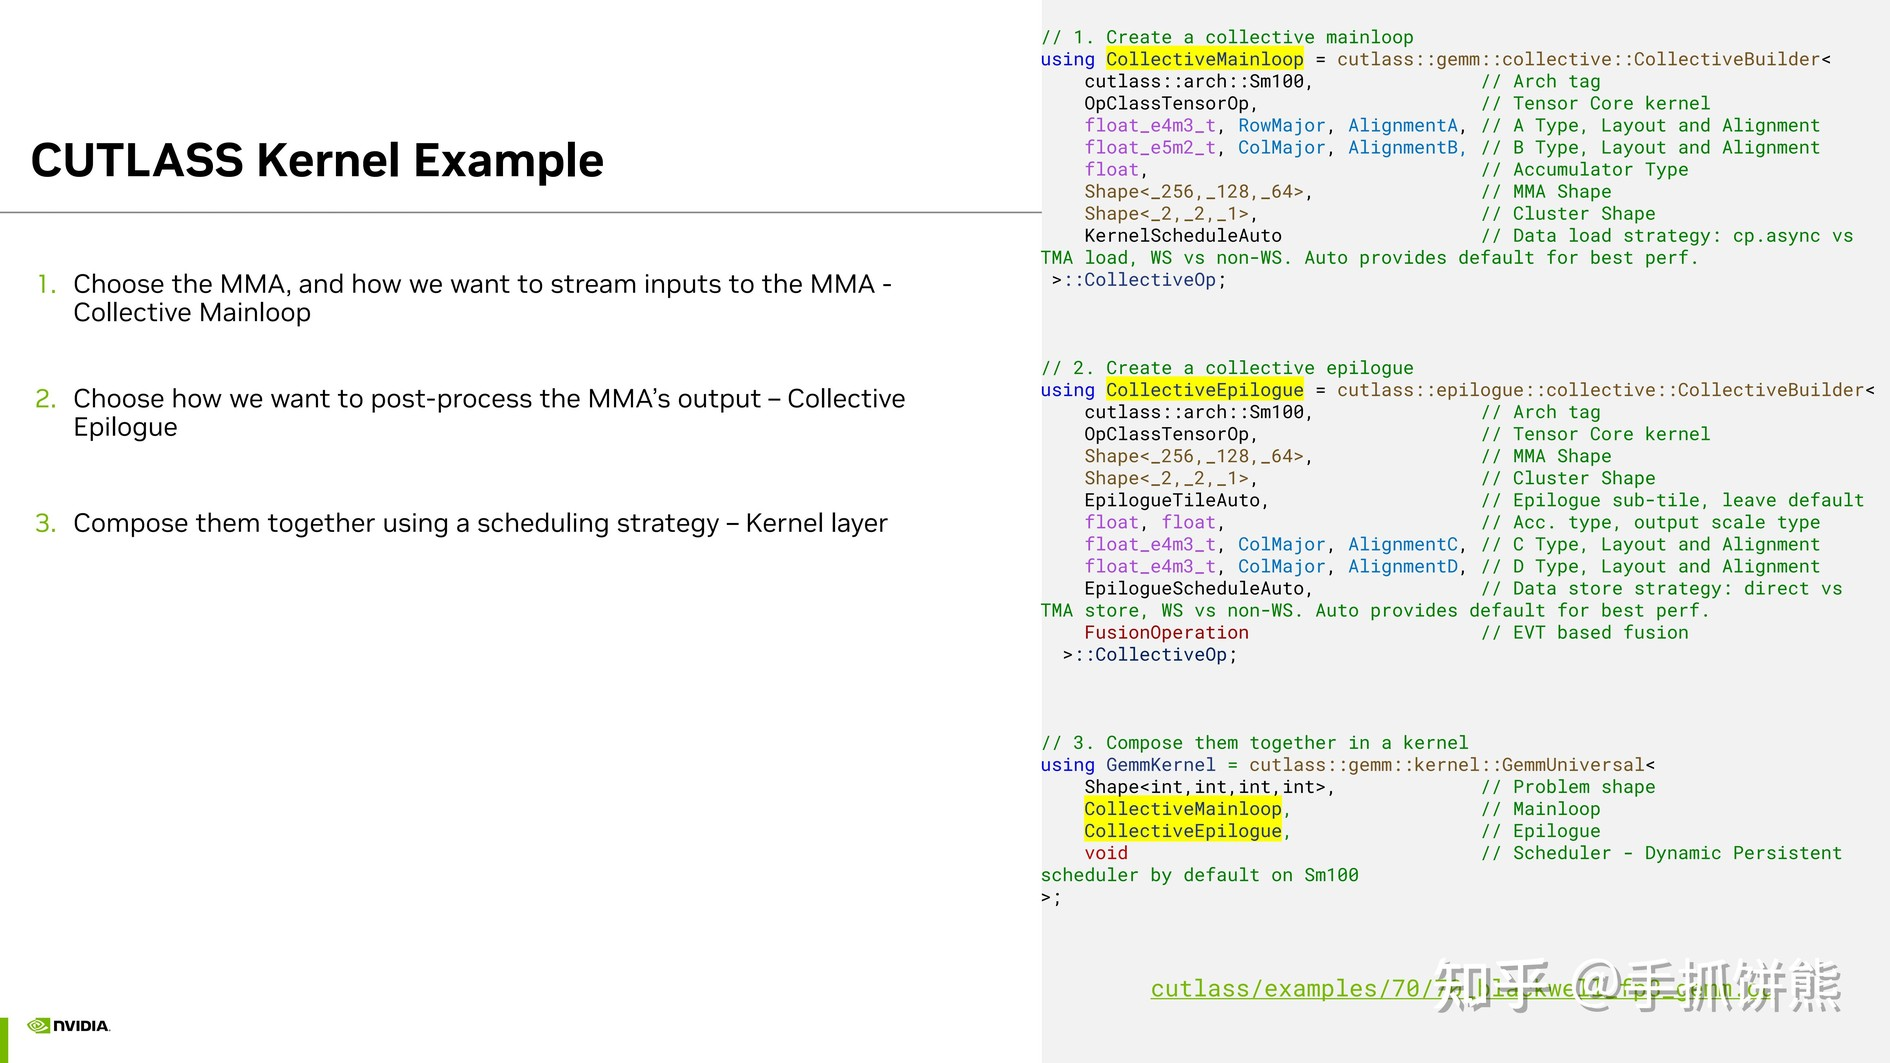
\includegraphics[width=0.9\textwidth]{figures/zhaoshangchun-01-tensor-core-programming/fig-55.jpg}
\end{figure}

\begin{itemize}
\item 使用 \texttt{c\allowbreak{}u\allowbreak{}t\allowbreak{}l\allowbreak{}a\allowbreak{}s\allowbreak{}s\allowbreak{}:\allowbreak{}:\allowbreak{}g\allowbreak{}e\allowbreak{}m\allowbreak{}m\allowbreak{}:\allowbreak{}:\allowbreak{}k\allowbreak{}e\allowbreak{}r\allowbreak{}n\allowbreak{}e\allowbreak{}l\allowbreak{}:\allowbreak{}:\allowbreak{}G\allowbreak{}e\allowbreak{}m\allowbreak{}m\allowbreak{}U\allowbreak{}n\allowbreak{}i\allowbreak{}v\allowbreak{}e\allowbreak{}r\allowbreak{}s\allowbreak{}a\allowbreak{}l}。
\item 将上面创建的 \texttt{Collective\allowbreak{}Mainloop} 和 \texttt{Collective\allowbreak{}Epilogue} 作为模板参数传入。
\item Scheduler 参数留空（\texttt{void}），在 Sm100 上会默认使用最高效的 \texttt{D\allowbreak{}y\allowbreak{}n\allowbreak{}a\allowbreak{}m\allowbreak{}i\allowbreak{}c\allowbreak{} \allowbreak{}P\allowbreak{}e\allowbreak{}r\allowbreak{}s\allowbreak{}i\allowbreak{}s\allowbreak{}t\allowbreak{}e\allowbreak{}n\allowbreak{}t\allowbreak{} \allowbreak{}S\allowbreak{}c\allowbreak{}h\allowbreak{}e\allowbreak{}d\allowbreak{}u\allowbreak{}l\allowbreak{}e\allowbreak{}r}。
\end{itemize}

CUTLASS Kernel 这个例子充分体现了 CUTLASS 3.x/\allowbreak{}4.x 声明式、面向意图的编程风格。

\begin{itemize}
\item \textbf{告别繁琐细节}：开发者只需要描述“我想要什么”（一个在 Sm100 上跑的、256x128 MMA、2x2 Cluster 的 FP8 GEMM），而无需关心“如何实现”（如何流水线、如何同步、如何管理 TMEM）。所有这些复杂性都被 Collective\allowbreak{}Builder 封装了。
\item \textbf{可读性与可维护性}：代码变得非常清晰。Mainloop、Epilogue、Kernel 的职责一目了然。当需要修改时，比如想换一种数据类型，或调整 MMA Shape，只需要修改相应的模板参数即可，无需重写整个内核。
\item \textbf{Auto 的威力}：Kernel\allowbreak{}Schedule\allowbreak{}Auto 和 Epilogue\allowbreak{}Schedule\allowbreak{}Auto 是非常有用的功能。它们背后是 NVIDIA 工程师的深度调优，可以为常见场景提供一个非常好的性能起点。只有在需要进行极限优化或处理特殊 case 时，我们才需要手动指定 Schedule。
\item \textbf{从 CTA Shape 到 MMA Shape}：注意，在 Sm100 的 Builder 中，我们指定的是 MMA Shape，而不是像 Sm90 (Hopper) 中那样指定 CTA Tile Shape。这是因为在 Blackwell 中，MMA 操作本身就可以跨越多个 CTA，MMA 的粒度比 CTA 更能反映计算的核心。
\end{itemize}

\textbf{第 57 页：一个完整的 CUTLASS 内核示例，从Hopper到Blackwell}

\begin{figure}[H]\centering
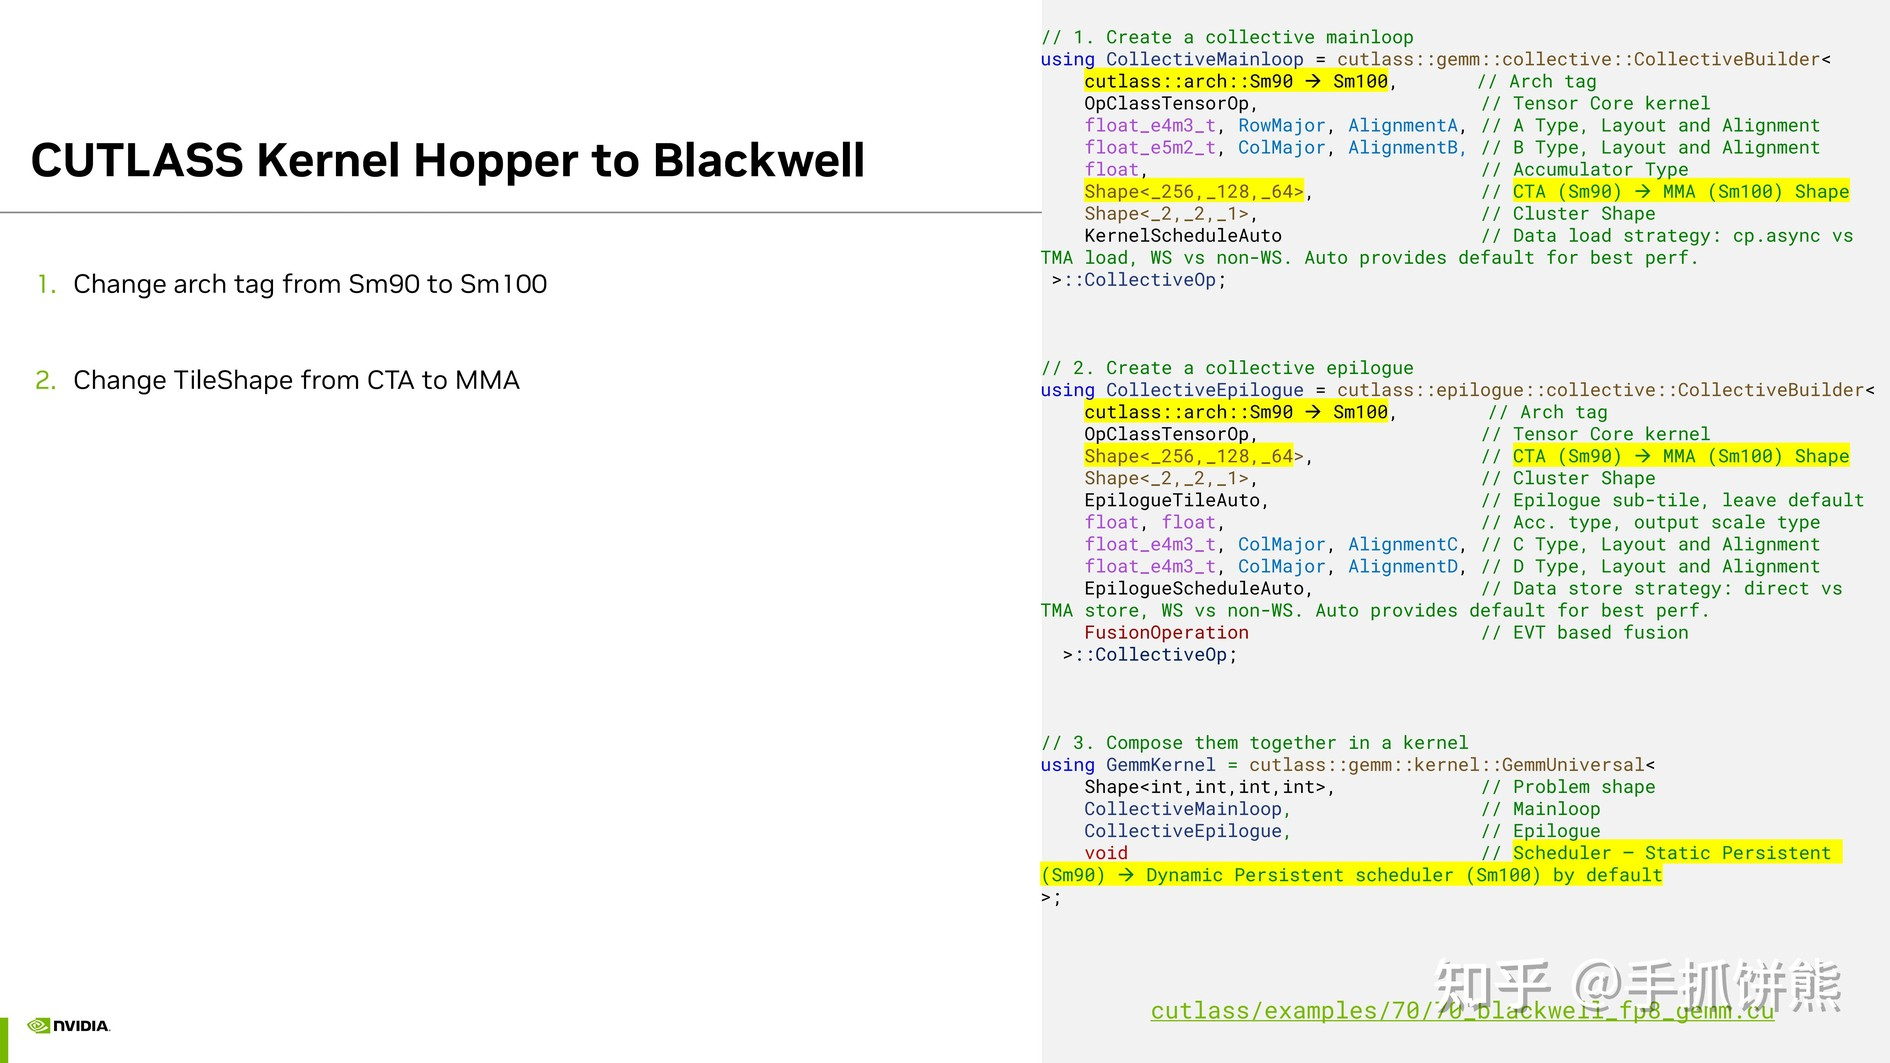
\includegraphics[width=0.9\textwidth]{figures/zhaoshangchun-01-tensor-core-programming/fig-56.jpg}
\end{figure}

这一页给出了将一个 Hopper (Sm90) CUTLASS 内核迁移到 Blackwell (Sm100) 的极简指南，只需两步：

\begin{enumerate}
\item \textbf{修改架构 Tag}：将 \texttt{cutlass::\allowbreak{}arch::\allowbreak{}Sm90} 改为 \texttt{cutlass::\allowbreak{}arch::\allowbreak{}Sm100}。
\item \textbf{修改 Tile Shape 语义}：在 \texttt{Collective\allowbreak{}Builder} 中，之前表示 \texttt{CTA Shape} 的 \texttt{Shape} 参数，现在语义变为了 \texttt{MMA Shape}。通常可以直接复用，因为 CUTLASS 会自动处理底层的差异。
\end{enumerate}

此外，调度器也会从 Sm90 默认的 \texttt{Static Persistent} 自动切换到 Sm100 默认的 \texttt{Dynamic Persistent}。

这展示了 CUTLASS 团队在保持 API 兼容性和平滑升级方面所做的巨大努力。

\begin{itemize}
\item \textbf{极低的迁移成本}：对于已经在使用 CUTLASS 3.x 的团队来说，升级到 Blackwell 的代码级工作量非常小。这使得我们可以快速地让现有应用享受到 Blackwell 带来的性能红利。
\item \textbf{抽象的力量}：之所以能实现如此平滑的迁移，是因为 CUTLASS 的高层抽象（\texttt{Collective\allowbreak{}Builder}）成功地将架构特异性（\texttt{Sm90} vs. \texttt{Sm100}）与通用逻辑（GEMM 算法）分离开来。当架构 tag 改变时，\texttt{Builder} 内部会切换到一套完全不同的、为 Blackwell 优化的底层实现，但对用户暴露的接口保持不变。
\item \textbf{性能“免费”午餐}：仅仅通过这两处简单的修改，内核就能自动用上 Blackwell 的新特性，如 \texttt{tcgen05.\allowbreak{}mma、TMEM} 累加器、动态调度等，从而获得接近 2 倍的性能提升。
\end{itemize}

\subsection{CUTLASS 的新features}

本小节将深入探索 CUTLASS 4.0 为 Blackwell 提供的预调优 “Collectives”，以及支持运行时动态配置等高级功能，展示其如何进一步提升性能和灵活性。

\textbf{第 58 页：Collective Mainloop and Builder}

\begin{figure}[H]\centering
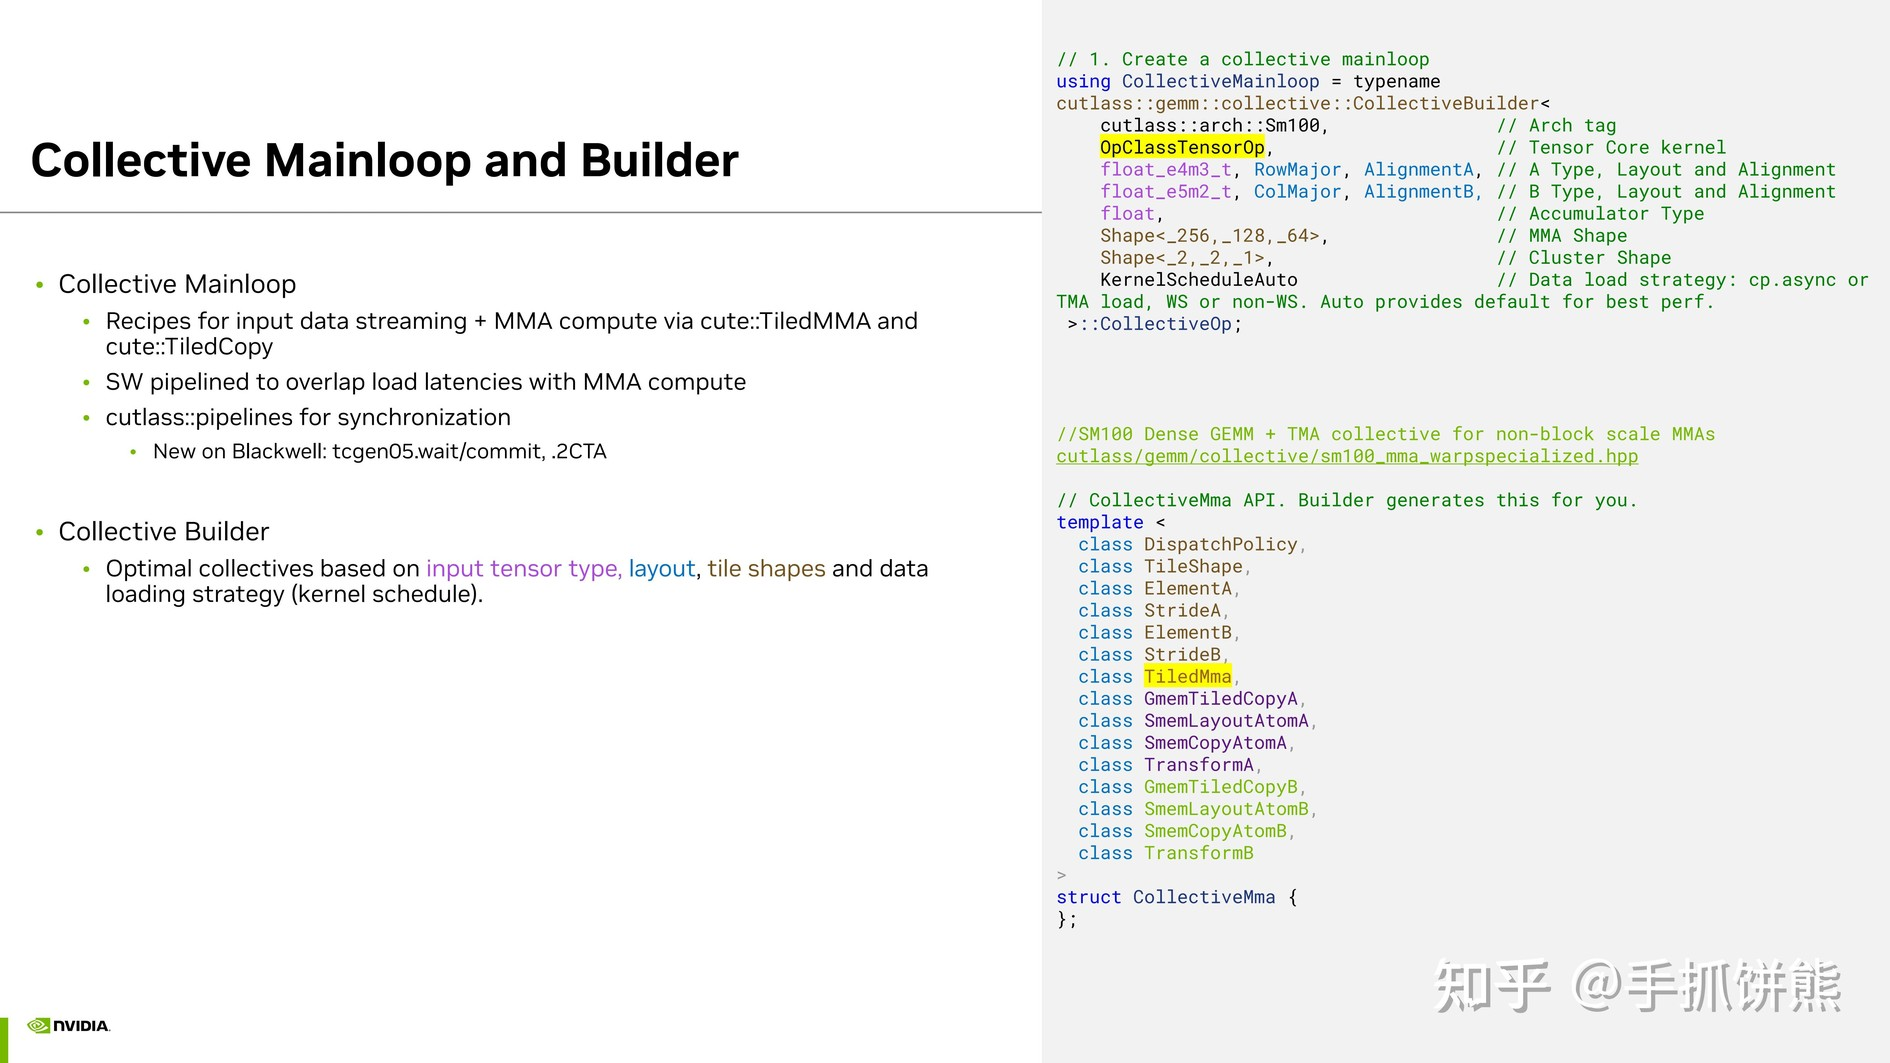
\includegraphics[width=0.9\textwidth]{figures/zhaoshangchun-01-tensor-core-programming/fig-57.jpg}
\end{figure}

这一页介绍了 CUTLASS 中\texttt{Collective\allowbreak{}Builder} 与 \texttt{Collective\allowbreak{}Mainloop}。其核心思想是\textbf{将复杂的高性能 GEMM（通用矩阵乘）主循环 (Mainloop) 的构建过程自动化、模板化}，让开发者从手动拼凑和调试复杂的 CUDA C++ 模板代码中解脱出来。以往，开发者需要像搭积木一样，手动选择数据加载、线程协作、MMA 指令等数十个模板参数来组成一个完整的 GEMM 内核，过程繁琐且极易出错。现在，\texttt{Collective\allowbreak{}Builder} 如同一个智能工厂，你只需要提供高级别的“规格需求”，它就能自动为你生成一个经过高度优化的 \texttt{Collective\allowbreak{}Mainloop} 实例。

深入来看 \texttt{Collective\allowbreak{}Builder} 的模板参数列表，这就像是在填写一张精密的“内核订单”。\texttt{cutlass::\allowbreak{}arch::\allowbreak{}Sm100} 明确了目标硬件是 Blackwell 架构，这使得 Builder 能够选用该架构专属的最新指令集和硬件单元，如第五代 Tensor Core (TCGen05)。数据类型（如 \texttt{float\_\allowbreak{}e4m3\_\allowbreak{}t}）和布局（\texttt{Row\allowbreak{}Major}）的指定，让 Builder 可以优化内存访问模式以最大化带宽。而 \texttt{MMA Shape}（如 \texttt{\_\allowbreak{}256,\allowbreak{}\_\allowbreak{}128,\allowbreak{}\_\allowbreak{}64}）和 \texttt{Cluster Shape}（如 \texttt{\_\allowbreak{}2,\allowbreak{}\_\allowbreak{}2,\allowbreak{}\_\allowbreak{}1}）则定义了内核的并行粒度，前者是单个线程块（Thread Block）处理的瓦块（Tile）大小，后者则利用 Blackwell 新增的\textbf{线程块集群 (Thread Block Cluster)} 特性，让多个线程块协同处理一个更大的计算任务，从而更好地摊分数据加载开销、提升算力利用率。最后，\texttt{Kernel\allowbreak{}Schedule\allowbreak{}Auto} 则将调度策略的选择权完全交给 CUTLASS，它会根据其他参数在 TMA（Tensor Memory Accelerator）和 \texttt{cp.\allowbreak{}async}、Warp-Specialized (WS) 和非 WS 之间做出最优选择，实现开箱即用的高性能。

\texttt{Collective\allowbreak{}Mma} 接口本身则是 CUTLASS 模块化设计的集中体现。它背后是由一系列遵循 Cu\allowbreak{}Te（CUDA Templates for Expressing Tensor Computations）编程模型的组件构成的“配方 (recipe)”。这些组件包括负责全局内存到共享内存数据搬运的 \texttt{Gmem\allowbreak{}Tiled\allowbreak{}Copy}、定义共享内存数据布局以避免 bank conflict 的 \texttt{Smem\allowbreak{}Layout\allowbreak{}Atom}、以及执行实际矩阵乘加运算的 \texttt{Tiled\allowbreak{}Mma} 等。整个 \texttt{Collective\allowbreak{}Mainloop} 通过精密的\textbf{软件流水线 (Software Pipelining)} 将数据加载 (load) 与计算 (compute) 深度重叠，有效隐藏了访存延迟。特别是在 Blackwell 架构上，新的同步原语 \texttt{tcgen05.\allowbreak{}wait/\allowbreak{}commit} 和支持多达 8 个 CTA 协作的 \texttt{mbarrier} 机制，让这种流水线可以扩展到整个 Cluster 层面，实现了前所未有的并行效率和性能。

\textbf{第 59 页：面向non-block scale MMA 的dense GEMM}

\begin{figure}[H]\centering
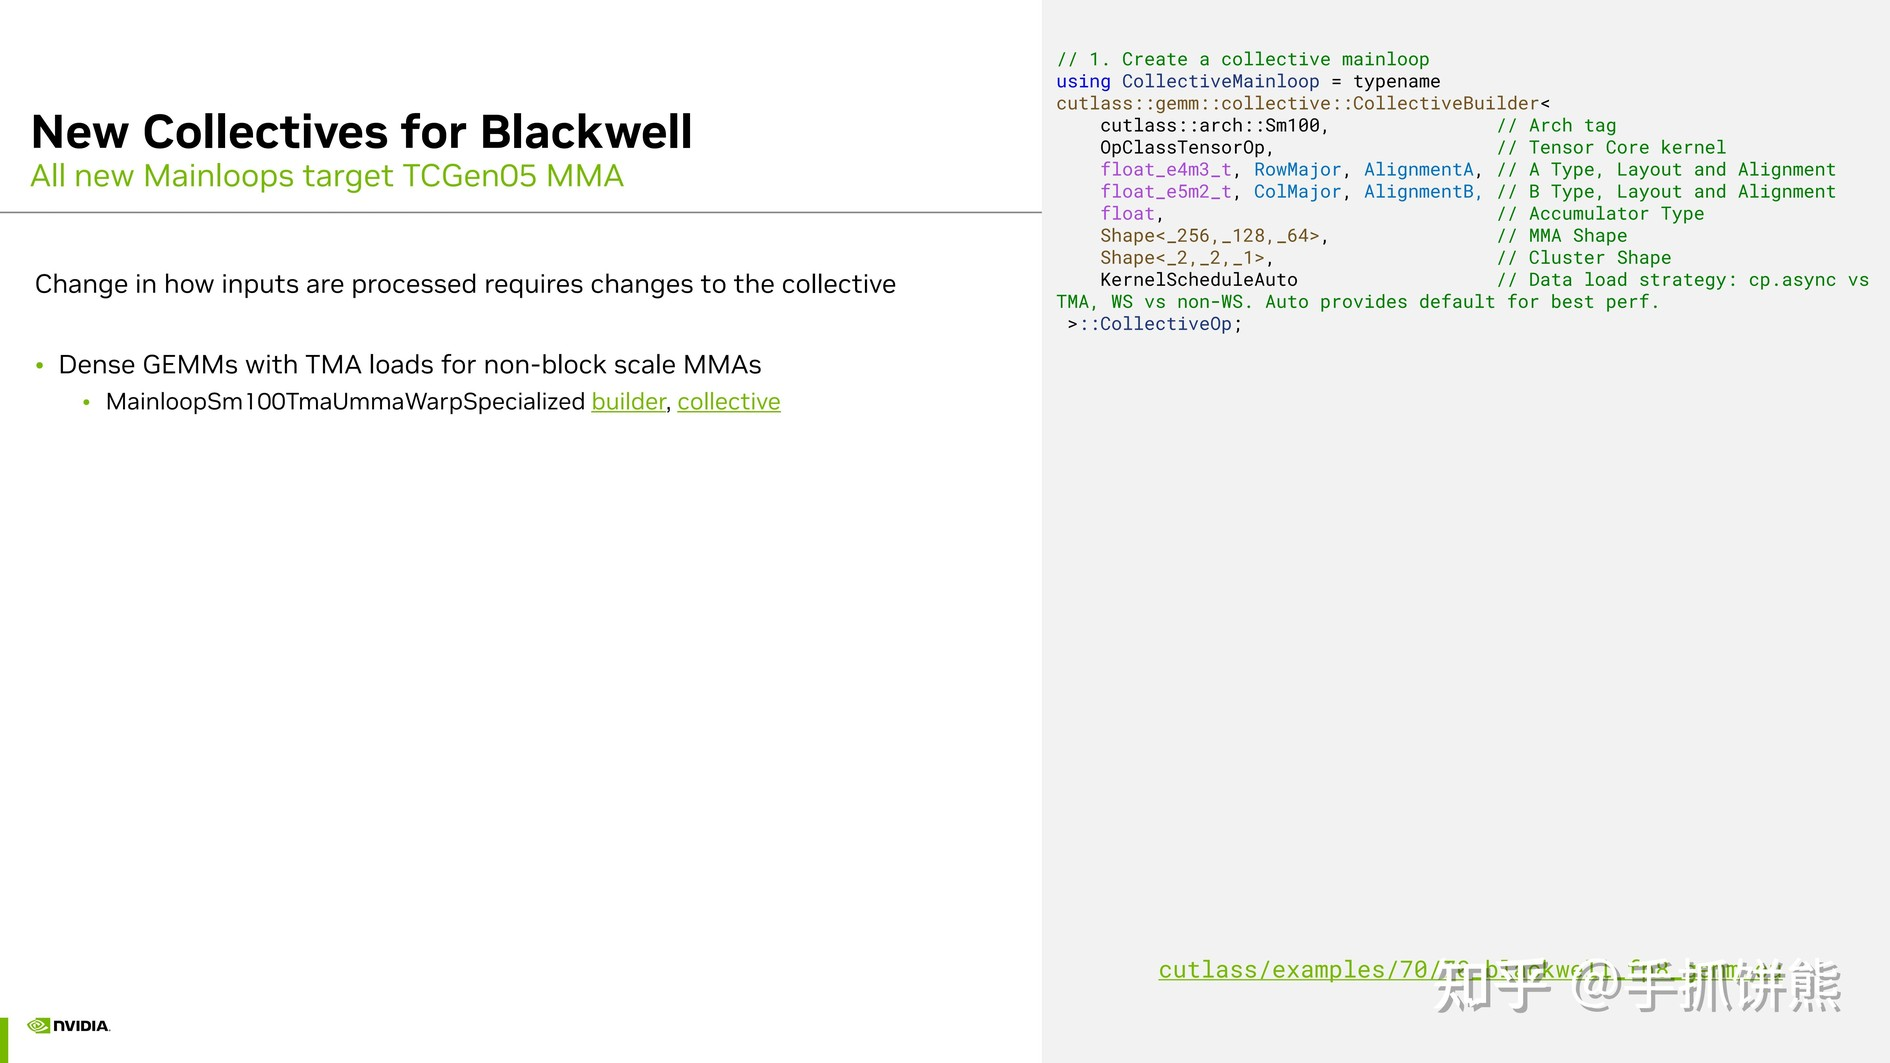
\includegraphics[width=0.9\textwidth]{figures/zhaoshangchun-01-tensor-core-programming/fig-58.jpg}
\end{figure}

这一页展示了 \texttt{Collective\allowbreak{}Builder} 的第一个具体应用场景：\textbf{为 non-block scale} \textbf{MMA 设计的Dense GEMM}。这里的 non-block scale 是相对于 Blackwell 架构新引入的硬件 block-scaling 特性而言的。它指的是那些缩放因子（scale）作用于per-tensor或某个维度 per-channel/\allowbreak{}per-token 的传统量化场景。例如，标准的 FP16、BF16 运算，以及大部分 per-tensor/\allowbreak{}per-channel 的 FP8/\allowbreak{}INT8 量化 GEMM，都属于这个范畴。在这类场景下，硬件执行的 MMA（Matrix Multiply-Accumulate）指令本身不直接处理缩放因子，相关的反量化操作通常在数据加载后、计算前由软件完成。

针对这一经典场景，CUTLASS 4.0 提供了一个预调优的 \texttt{collective} 实现，名为 \texttt{M\allowbreak{}a\allowbreak{}i\allowbreak{}n\allowbreak{}l\allowbreak{}o\allowbreak{}o\allowbreak{}p\allowbreak{}S\allowbreak{}m\allowbreak{}1\allowbreak{}0\allowbreak{}0\allowbreak{}T\allowbreak{}m\allowbreak{}a\allowbreak{}U\allowbreak{}m\allowbreak{}m\allowbreak{}a\allowbreak{}W\allowbreak{}a\allowbreak{}r\allowbreak{}p\allowbreak{}S\allowbreak{}p\allowbreak{}e\allowbreak{}c\allowbreak{}i\allowbreak{}a\allowbreak{}l\allowbreak{}i\allowbreak{}z\allowbreak{}e\allowbreak{}d}。这个命名本身就是一份详尽的技术规格书：\texttt{Sm100} 指明它为 Blackwell 优化；\texttt{Tma} 表示数据从全局内存到共享内存的加载路径采用了\textbf{硬件加速的 TMA (Tensor Memory Accelerator)}，这是 Blackwell 提升访存效率的核心武器；\texttt{Umma} (Unified MMA) 则代表内核的计算核心使用了 Blackwell 上统一的、面向第五代 Tensor Core (TCGen05) 的 MMA 指令接口；而 \texttt{Warp\allowbreak{}Specialized} (WS) 则是一种高效的\textbf{软件流水线调度策略}，它将线程块内的 warps 分为生产者（负责数据加载）和消费者（负责计算），两者通过共享内存和精巧的同步机制并行工作，以最大程度地隐藏访存延迟。

此页右侧的代码片段与上一页基本一致，但其意图在于强调，对于开发者而言，即使是这样一个看似传统的 GEMM 场景，其底层的 \texttt{collective} 实现也已全面升级，以充分利用 Blackwell 的新硬件特性。\texttt{70\_\allowbreak{}blackwell\_\allowbreak{}fp8\_\allowbreak{}gemm.\allowbreak{}cu} 这个示例工程就是最佳证明。它为开发者提供了一个标准的、高性能的 FP8 GEMM 实现范本，展示了如何配置 \texttt{Collective\allowbreak{}Builder} 来生成一个适用于稠密 FP8 推理或训练的内核。从工程实践角度看，这意味着开发者在 Blackwell 上处理标准 GEMM 任务时，无需从零开始，可以直接复用这个\textbf{官方“最佳实践”}，将其作为性能基线和二次开发的基础，从而大大加速研发进程。

\textbf{第 60 页：面向 block-scaling MMA 的 Dense GEMM}

\begin{figure}[H]\centering
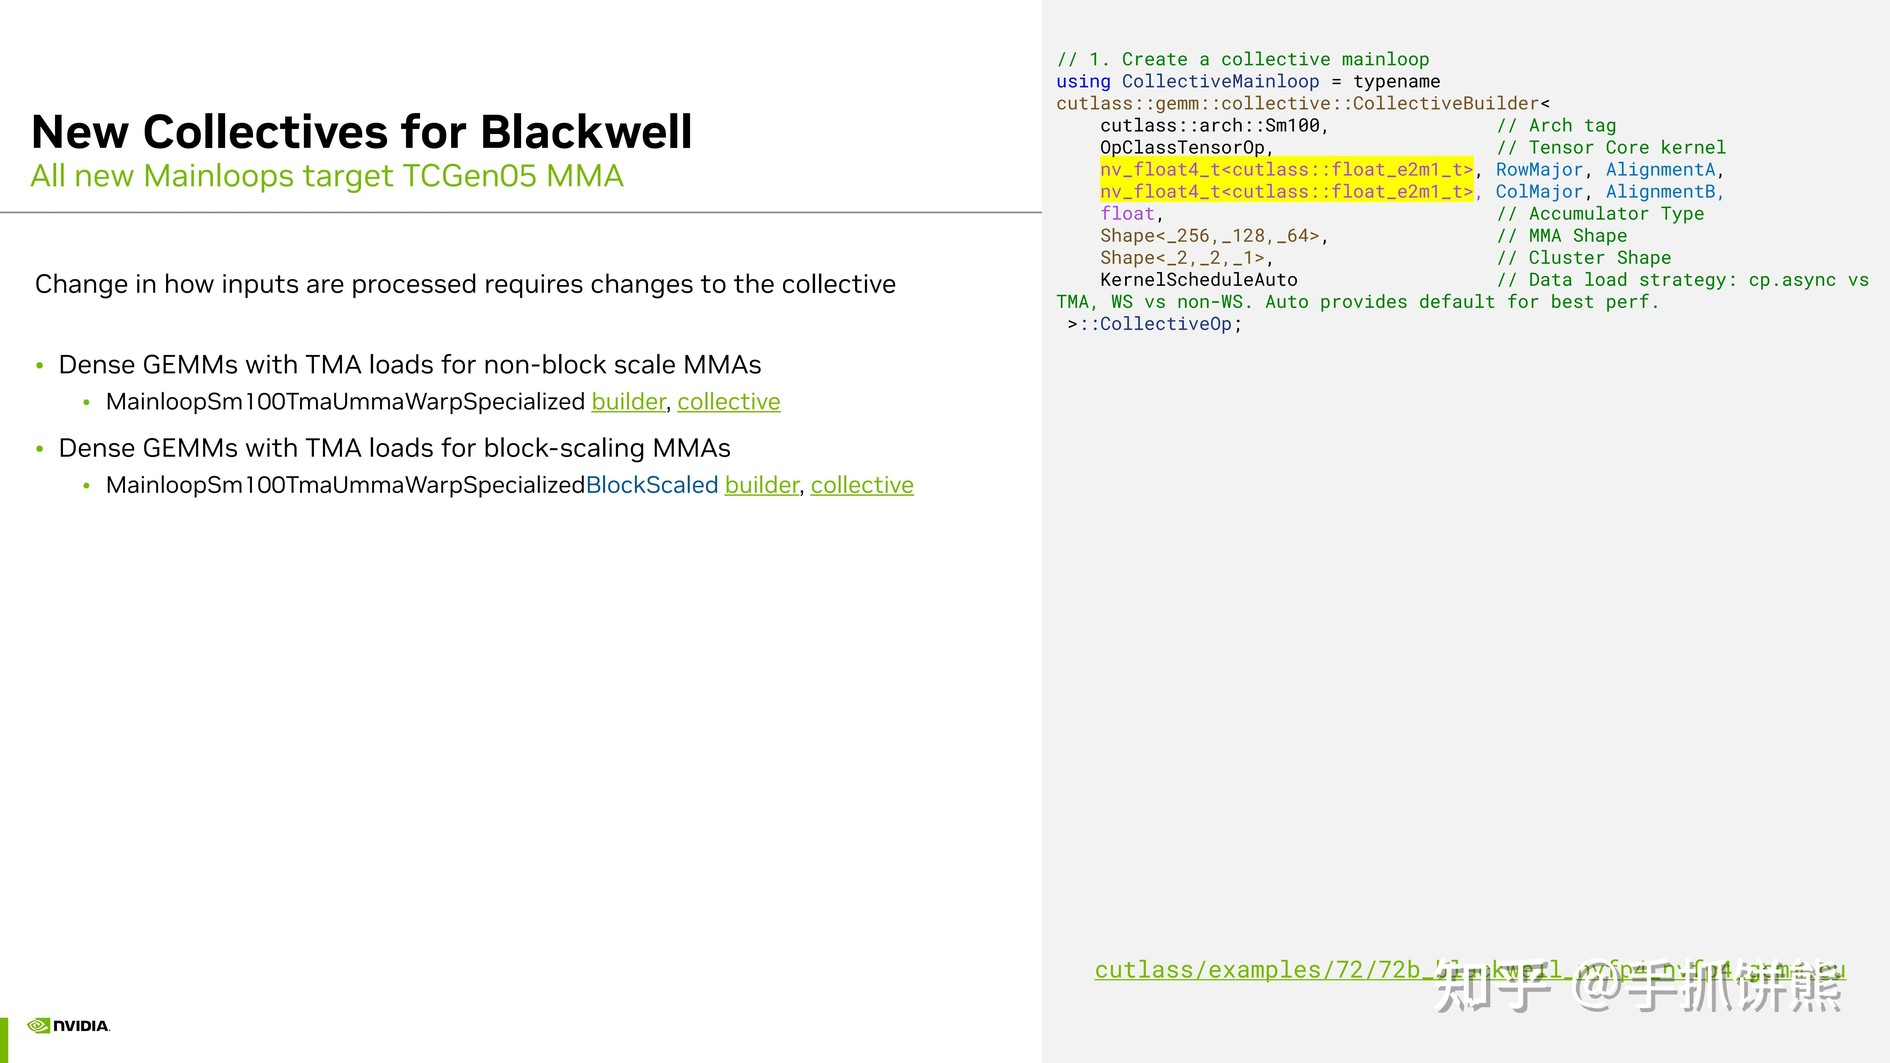
\includegraphics[width=0.9\textwidth]{figures/zhaoshangchun-01-tensor-core-programming/fig-59.jpg}
\end{figure}

本页聚焦于 \texttt{Collective\allowbreak{}Builder} 的第二个关键用例：\textbf{为支持硬件 block-scaling 的 MMA 设计的Dense GEMM}。这直接命中了 Blackwell 架构在低精度计算领域的一大核心升级。与上一代 Hopper 架构相比，Blackwell 的第五代 Tensor Core 引入了对\textbf{每个数据块（data block）独立的缩放因子（scale）的硬件原生支持}。这意味着在执行 FP8 或 FP4/\allowbreak{}NVFP4 这类超低精度矩阵乘法时，硬件可以在计算过程中直接、高效地处理与每个细粒度数据块相关联的元数据（即缩放因子），而无需软件在计算前进行显式的、代价高昂的反量化操作。这对于在极限压缩模型体积和内存带宽的同时，最大程度保持数值精度和动态范围至关重要。

为了无缝对接这一硬件特性，CUTLASS 4.0 提供了 \texttt{M\allowbreak{}a\allowbreak{}i\allowbreak{}n\allowbreak{}l\allowbreak{}o\allowbreak{}o\allowbreak{}p\allowbreak{}S\allowbreak{}m\allowbreak{}1\allowbreak{}0\allowbreak{}0\allowbreak{}T\allowbreak{}m\allowbreak{}a\allowbreak{}U\allowbreak{}m\allowbreak{}m\allowbreak{}a\allowbreak{}W\allowbreak{}a\allowbreak{}r\allowbreak{}p\allowbreak{}S\allowbreak{}p\allowbreak{}e\allowbreak{}c\allowbreak{}i\allowbreak{}a\allowbreak{}l\allowbreak{}i\allowbreak{}z\allowbreak{}e\allowbreak{}d\allowbreak{}B\allowbreak{}l\allowbreak{}o\allowbreak{}c\allowbreak{}k\allowbreak{}S\allowbreak{}c\allowbreak{}a\allowbreak{}l\allowbreak{}e\allowbreak{}d} 这一特定的 \texttt{collective}。这个 \texttt{collective} 的内部实现，特别是其 \texttt{Tiled\allowbreak{}Mma} 部分，被精心设计用来与 TCGen05 的块缩放功能协同工作。它会自动处理块缩放元数据的加载、分发和在 MMA 指令中的应用，将复杂的硬件交互细节完全封装起来，对上层开发者透明。这使得开发者能够像使用普通 GEMM 一样，轻松地利用这一强大的新硬件特性。

代码示例中，输入张量 A 和 B 的类型从 \texttt{float\_\allowbreak{}e4m3\_\allowbreak{}t} 变成了 \texttt{n\allowbreak{}v\allowbreak{}\_\allowbreak{}f\allowbreak{}l\allowbreak{}o\allowbreak{}a\allowbreak{}t\allowbreak{}4\allowbreak{}\_\allowbreak{}t\allowbreak{}<\allowbreak{}c\allowbreak{}u\allowbreak{}t\allowbreak{}l\allowbreak{}a\allowbreak{}s\allowbreak{}s\allowbreak{}:\allowbreak{}:\allowbreak{}f\allowbreak{}l\allowbreak{}o\allowbreak{}a\allowbreak{}t\allowbreak{}\_\allowbreak{}e\allowbreak{}2\allowbreak{}m\allowbreak{}1\allowbreak{}\_\allowbreak{}t\allowbreak{}>}，这表明我们正在处理 \textbf{NVFP4}（一种 4-bit 浮点格式）。这种数据类型每个字节可以存储两个 4-bit 数值，将内存占用和带宽需求压缩到了极致。\texttt{7\allowbreak{}2\allowbreak{}b\allowbreak{}\_\allowbreak{}b\allowbreak{}l\allowbreak{}a\allowbreak{}c\allowbreak{}k\allowbreak{}w\allowbreak{}e\allowbreak{}l\allowbreak{}l\allowbreak{}\_\allowbreak{}n\allowbreak{}v\allowbreak{}f\allowbreak{}p\allowbreak{}4\allowbreak{}\_\allowbreak{}n\allowbreak{}v\allowbreak{}f\allowbreak{}p\allowbreak{}4\allowbreak{}\_\allowbreak{}g\allowbreak{}e\allowbreak{}m\allowbreak{}m\allowbreak{}.\allowbreak{}c\allowbreak{}u} 这个示例工程的意义非凡，它揭示了 Blackwell 在大模型\textbf{推理场景下的巨大潜力}。通过 NVFP4 和硬件块缩放的结合，可以在可接受的精度损失下，将模型权重占用的显存减半（相较于 FP8），并显著提升访存密集型算子的执行效率。对于动辄数千亿甚至万亿参数的巨型模型而言，这意味着更低的部署成本和更高的推理吞吐量，是推动 AI 服务普惠化的关键技术之一。

\textbf{第 61 页：面向 Dense Grouped GEMM}

\begin{figure}[H]\centering
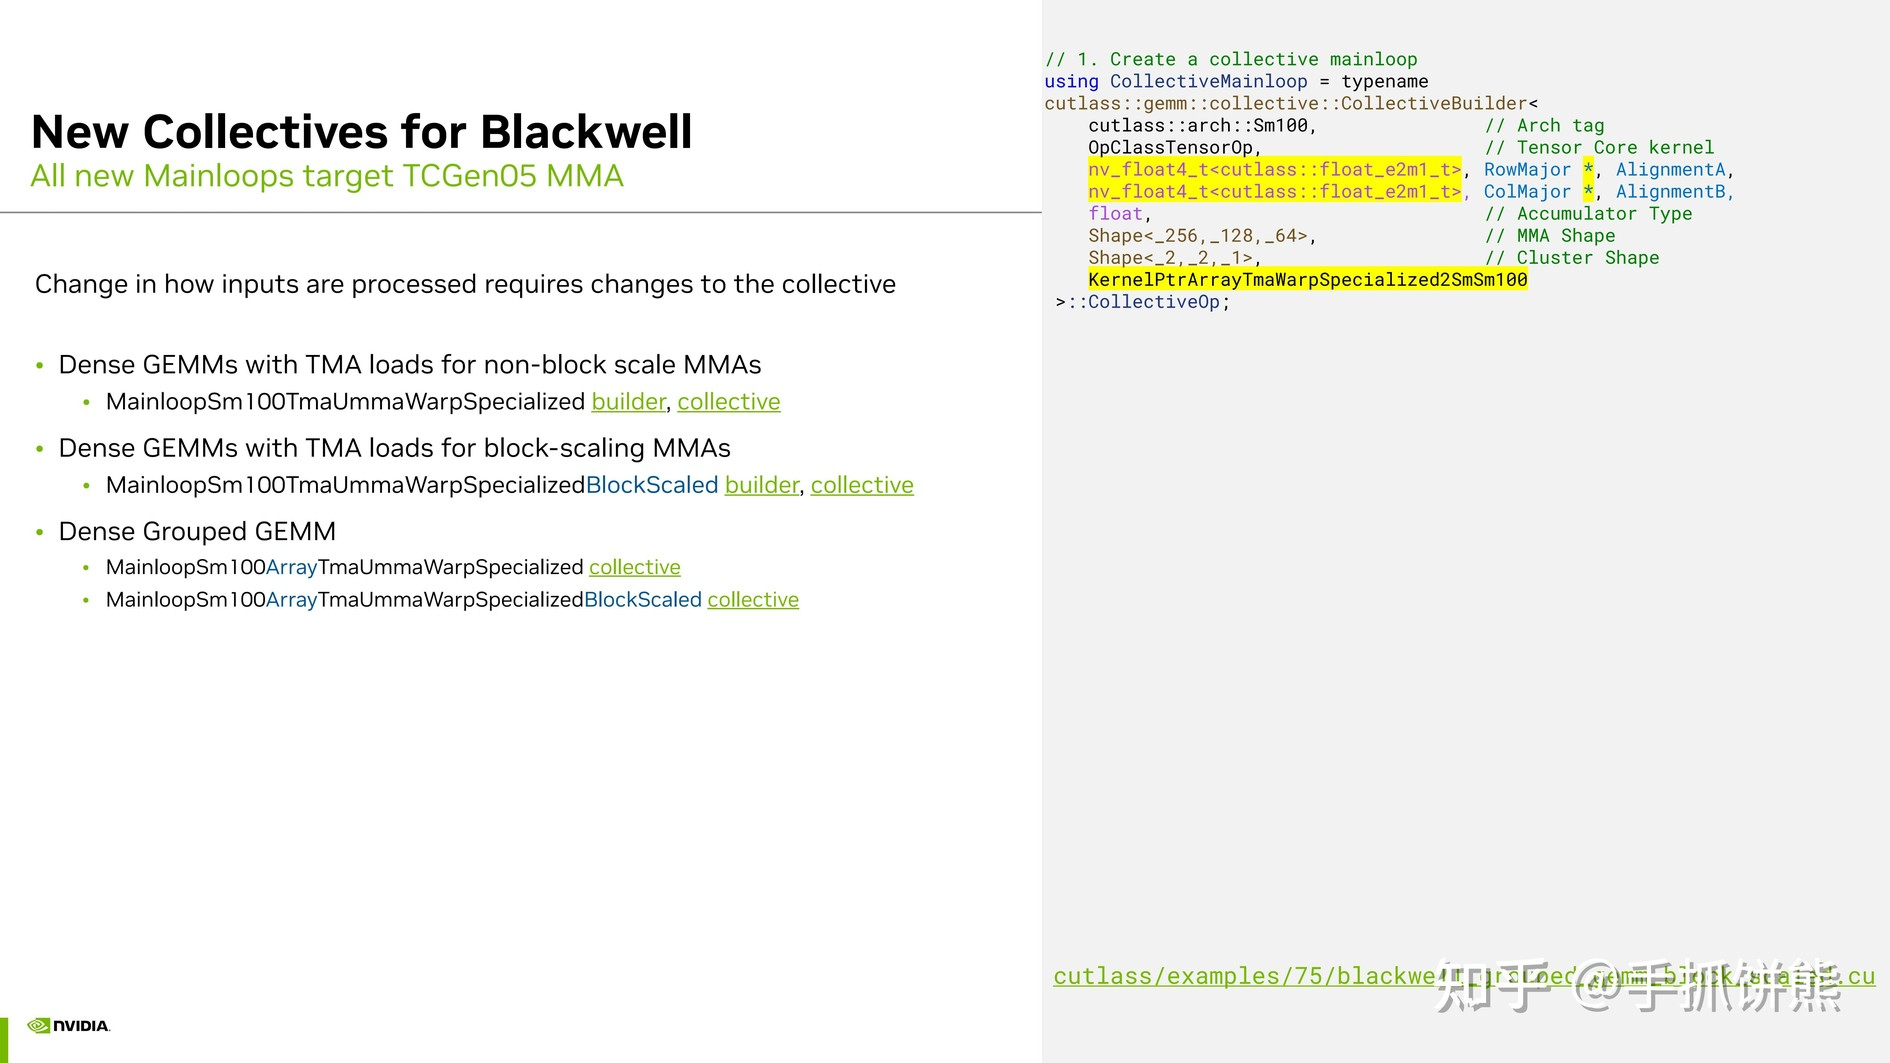
\includegraphics[width=0.9\textwidth]{figures/zhaoshangchun-01-tensor-core-programming/fig-60.jpg}
\end{figure}

幻灯片进入了第三个核心应用场景：Dense Grouped GEMM。这是一种在现代深度学习模型，尤其是 Transformer 架构中日益普及的计算模式。它专门解决“一次性执行大量形状各异的小型矩阵乘法”的问题。典型的应用包括：在\textbf{混合专家模型 (Mixture-of-Experts, Mo\allowbreak{}E)} 中，输入 token 被路由到不同的“专家”（每个专家都是一个小型前馈网络），导致了批处理维度上的 GEMM 被拆分成一组小 GEMM。如果为每个小 GEMM 单独启动一个 CUDA kernel，高昂的启动开销和 GPU 资源的低利用率将导致性能瓶颈。Grouped GEMM 则通过将这些小问题“打包”到一次 kernel 启动中，来摊销开销并提升整体吞吐。

CUTLASS 4.0 为此提供了 \texttt{M\allowbreak{}a\allowbreak{}i\allowbreak{}n\allowbreak{}l\allowbreak{}o\allowbreak{}o\allowbreak{}p\allowbreak{}S\allowbreak{}m\allowbreak{}1\allowbreak{}0\allowbreak{}0\allowbreak{}A\allowbreak{}r\allowbreak{}r\allowbreak{}a\allowbreak{}y\allowbreak{}T\allowbreak{}m\allowbreak{}a\allowbreak{}U\allowbreak{}m\allowbreak{}m\allowbreak{}a\allowbreak{}W\allowbreak{}a\allowbreak{}r\allowbreak{}p\allowbreak{}S\allowbreak{}p\allowbreak{}e\allowbreak{}c\allowbreak{}i\allowbreak{}a\allowbreak{}l\allowbreak{}i\allowbreak{}z\allowbreak{}e\allowbreak{}d} 和 \texttt{M\allowbreak{}a\allowbreak{}i\allowbreak{}n\allowbreak{}l\allowbreak{}o\allowbreak{}o\allowbreak{}p\allowbreak{}S\allowbreak{}m\allowbreak{}1\allowbreak{}0\allowbreak{}0\allowbreak{}A\allowbreak{}r\allowbreak{}r\allowbreak{}a\allowbreak{}y\allowbreak{}T\allowbreak{}m\allowbreak{}a\allowbreak{}U\allowbreak{}m\allowbreak{}m\allowbreak{}a\allowbreak{}W\allowbreak{}a\allowbreak{}r\allowbreak{}p\allowbreak{}S\allowbreak{}p\allowbreak{}e\allowbreak{}c\allowbreak{}i\allowbreak{}a\allowbreak{}l\allowbreak{}i\allowbreak{}z\allowbreak{}e\allowbreak{}d\allowbreak{}B\allowbreak{}l\allowbreak{}o\allowbreak{}c\allowbreak{}k\allowbreak{}S\allowbreak{}c\allowbreak{}a\allowbreak{}l\allowbreak{}e\allowbreak{}d} 两个版本的 \texttt{collective}。这里的关键词是 \texttt{Array}。它表示这个 \texttt{mainloop} 能够接收一个\textbf{问题描述符数组 (array of problem descriptors)} 作为输入，数组中的每个元素描述了一个独立的 GEMM 子问题（如矩阵的指针、维度、leading dimension 等）。内核的调度逻辑会遍历这个数组，让线程块（或线程块集群）动态地认领并执行这些子问题。这种设计极大地提升了灵活性和效率。同时，提供 \texttt{Block\allowbreak{}Scaled} 版本也意味着 Grouped GEMM 可以与 Blackwell 的硬件块缩放特性无缝结合，为量化版的 Mo\allowbreak{}E 等模型提供最优支持。

在代码层面，一个显著的变化是 A 和 B 矩阵的布局被指定为 \texttt{Row\allowbreak{}Major*} 和 \texttt{Col\allowbreak{}Major*}（注意星号），并且 \texttt{Kernel\allowbreak{}Schedule} 变成了 \texttt{K\allowbreak{}e\allowbreak{}r\allowbreak{}n\allowbreak{}e\allowbreak{}l\allowbreak{}P\allowbreak{}t\allowbreak{}r\allowbreak{}A\allowbreak{}r\allowbreak{}r\allowbreak{}a\allowbreak{}y\allowbreak{}T\allowbreak{}m\allowbreak{}a\allowbreak{}W\allowbreak{}a\allowbreak{}r\allowbreak{}p\allowbreak{}S\allowbreak{}p\allowbreak{}e\allowbreak{}c\allowbreak{}i\allowbreak{}a\allowbreak{}l\allowbreak{}i\allowbreak{}z\allowbreak{}e\allowbreak{}d\allowbreak{}2\allowbreak{}S\allowbreak{}m\allowbreak{}S\allowbreak{}m\allowbreak{}1\allowbreak{}0\allowbreak{}0}。这暗示了内核现在处理的是\textbf{指向不同矩阵的指针数组}，而非单个矩阵指针。示例 \texttt{7\allowbreak{}5\allowbreak{}\_\allowbreak{}b\allowbreak{}l\allowbreak{}a\allowbreak{}c\allowbreak{}k\allowbreak{}w\allowbreak{}e\allowbreak{}l\allowbreak{}l\allowbreak{}\_\allowbreak{}g\allowbreak{}r\allowbreak{}o\allowbreak{}u\allowbreak{}p\allowbreak{}e\allowbreak{}d\allowbreak{}\_\allowbreak{}g\allowbreak{}e\allowbreak{}m\allowbreak{}m\allowbreak{}\_\allowbreak{}b\allowbreak{}l\allowbreak{}o\allowbreak{}c\allowbreak{}k\allowbreak{}\_\allowbreak{}s\allowbreak{}c\allowbreak{}a\allowbreak{}l\allowbreak{}e\allowbreak{}d\allowbreak{}.\allowbreak{}c\allowbreak{}u} 完美地诠释了这种能力的强大之处。它将 Grouped GEMM 和 Block-Scaling 两大特性结合，为在 Blackwell 上高效运行大规模、超低精度的 Mo\allowbreak{}E 模型铺平了道路。这不仅是性能的提升，更是一种\textbf{编程范式的演进}，它允许开发者以更集合化、更高层的方式来描述和优化这类复杂的、异构的并行计算任务，显著降低了工程实现的复杂度。

\textbf{第 62 页：CUTLASS 预调优的 Mainloop Collectives 汇总}

\begin{figure}[H]\centering
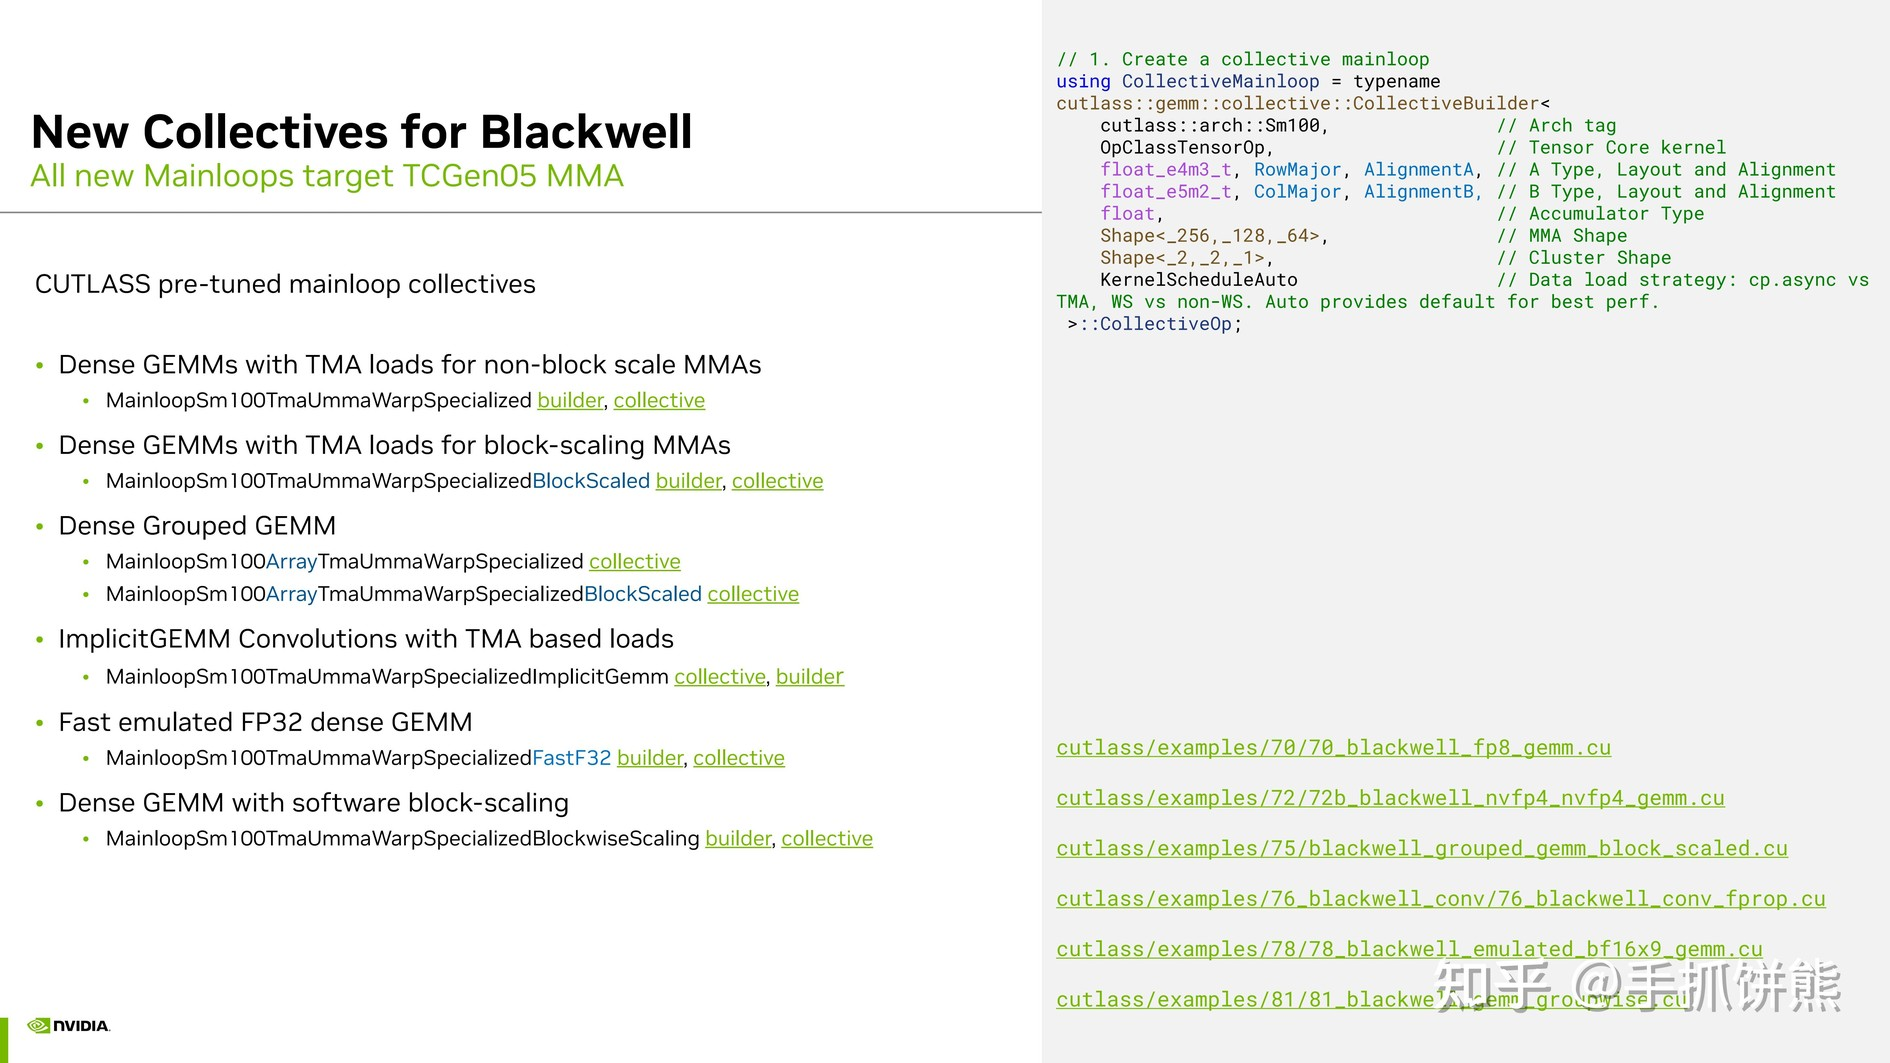
\includegraphics[width=0.9\textwidth]{figures/zhaoshangchun-01-tensor-core-programming/fig-61.jpg}
\end{figure}

这一页可以被视为 CUTLASS 4.0 在 Blackwell 架构上的\textbf{“能力清单”和“最佳实践指南”}。它系统性地汇总了为不同主流计算场景所设计的、经过预调优的 \texttt{mainloop collectives}。这传达出一个核心的工程信号：对于绝大多数在 Blackwell 上的高性能计算需求，开发者不再需要从零开始“造轮子”，而是应该首先从这里中挑选最匹配自己需求。

除了前面几页已经深入分析过的三个核心场景（Dense GEMM、block-scaling GEMM、Grouped GEMM），这张列表还揭示了 CUTLASS 对更多复杂应用的内置支持。例如，\textbf{\texttt{I\allowbreak{}m\allowbreak{}p\allowbreak{}l\allowbreak{}i\allowbreak{}c\allowbreak{}i\allowbreak{}t\allowbreak{}G\allowbreak{}E\allowbreak{}M\allowbreak{}M\allowbreak{} \allowbreak{}C\allowbreak{}o\allowbreak{}n\allowbreak{}v\allowbreak{}o\allowbreak{}l\allowbreak{}u\allowbreak{}t\allowbreak{}i\allowbreak{}o\allowbreak{}n\allowbreak{}s\allowbreak{} \allowbreak{}w\allowbreak{}i\allowbreak{}t\allowbreak{}h\allowbreak{} \allowbreak{}T\allowbreak{}M\allowbreak{}A\allowbreak{} \allowbreak{}b\allowbreak{}a\allowbreak{}s\allowbreak{}e\allowbreak{}d\allowbreak{} \allowbreak{}l\allowbreak{}o\allowbreak{}a\allowbreak{}d\allowbreak{}s}} 展示了 CUTLASS 如何通过 \texttt{im2col} 或 \texttt{im2col-like} 的技术，将卷积运算巧妙地转化为 GEMM 问题，从而让卷积算子也能充分利用为 GEMM 设计的、高度优化的 TMA 数据加载路径和 Tensor Core 计算流水线。\textbf{\texttt{F\allowbreak{}a\allowbreak{}s\allowbreak{}t\allowbreak{} \allowbreak{}e\allowbreak{}m\allowbreak{}u\allowbreak{}l\allowbreak{}a\allowbreak{}t\allowbreak{}e\allowbreak{}d\allowbreak{} \allowbreak{}F\allowbreak{}P\allowbreak{}3\allowbreak{}2\allowbreak{} \allowbreak{}d\allowbreak{}e\allowbreak{}n\allowbreak{}s\allowbreak{}e\allowbreak{} \allowbreak{}G\allowbreak{}E\allowbreak{}M\allowbreak{}M}} 则提供了一种性能与精度权衡的方案：利用低精度（如 FP16/\allowbreak{}BF16）硬件的高吞吐特性来模拟 FP32 运算，从而在某些对精度不极端敏感的场景下获得远超原生 FP32 性能的加速。

此外，\textbf{\texttt{D\allowbreak{}e\allowbreak{}n\allowbreak{}s\allowbreak{}e\allowbreak{} \allowbreak{}G\allowbreak{}E\allowbreak{}M\allowbreak{}M\allowbreak{} \allowbreak{}w\allowbreak{}i\allowbreak{}t\allowbreak{}h\allowbreak{} \allowbreak{}s\allowbreak{}o\allowbreak{}f\allowbreak{}t\allowbreak{}w\allowbreak{}a\allowbreak{}r\allowbreak{}e\allowbreak{} \allowbreak{}b\allowbreak{}l\allowbreak{}o\allowbreak{}c\allowbreak{}k\allowbreak{}-\allowbreak{}s\allowbreak{}c\allowbreak{}a\allowbreak{}l\allowbreak{}i\allowbreak{}n\allowbreak{}g}} 提供了硬件块缩放之外的另一种选择。当模型需要的缩放粒度或模式是硬件不直接支持的特殊情况时，这个 \texttt{collective} 允许开发者在软件层面实现自定义的块缩放逻辑。虽然这会带来一些额外的指令开销，但它提供了极致的灵活性，使得各种新颖的量化算法也能在 CUTLASS 框架下快速实现和验证。从一名 GPU 工程师的角度来看，这张幻灯片的价值在于它极大地\textbf{降低了在 Blackwell 上进行高性能内核开发的门槛}。它提供了一个极高的性能起点，开发者只需通过 \texttt{Collective\allowbreak{}Builder} 进行简单的“声明式”配置，就能获得接近手写汇编级别的优化效果，从而可以将更多精力聚焦于上层算法和模型的创新。

\textbf{第 63 页：Mainloop Builder 的新特性 — 运行时配置与组合}

\begin{figure}[H]\centering
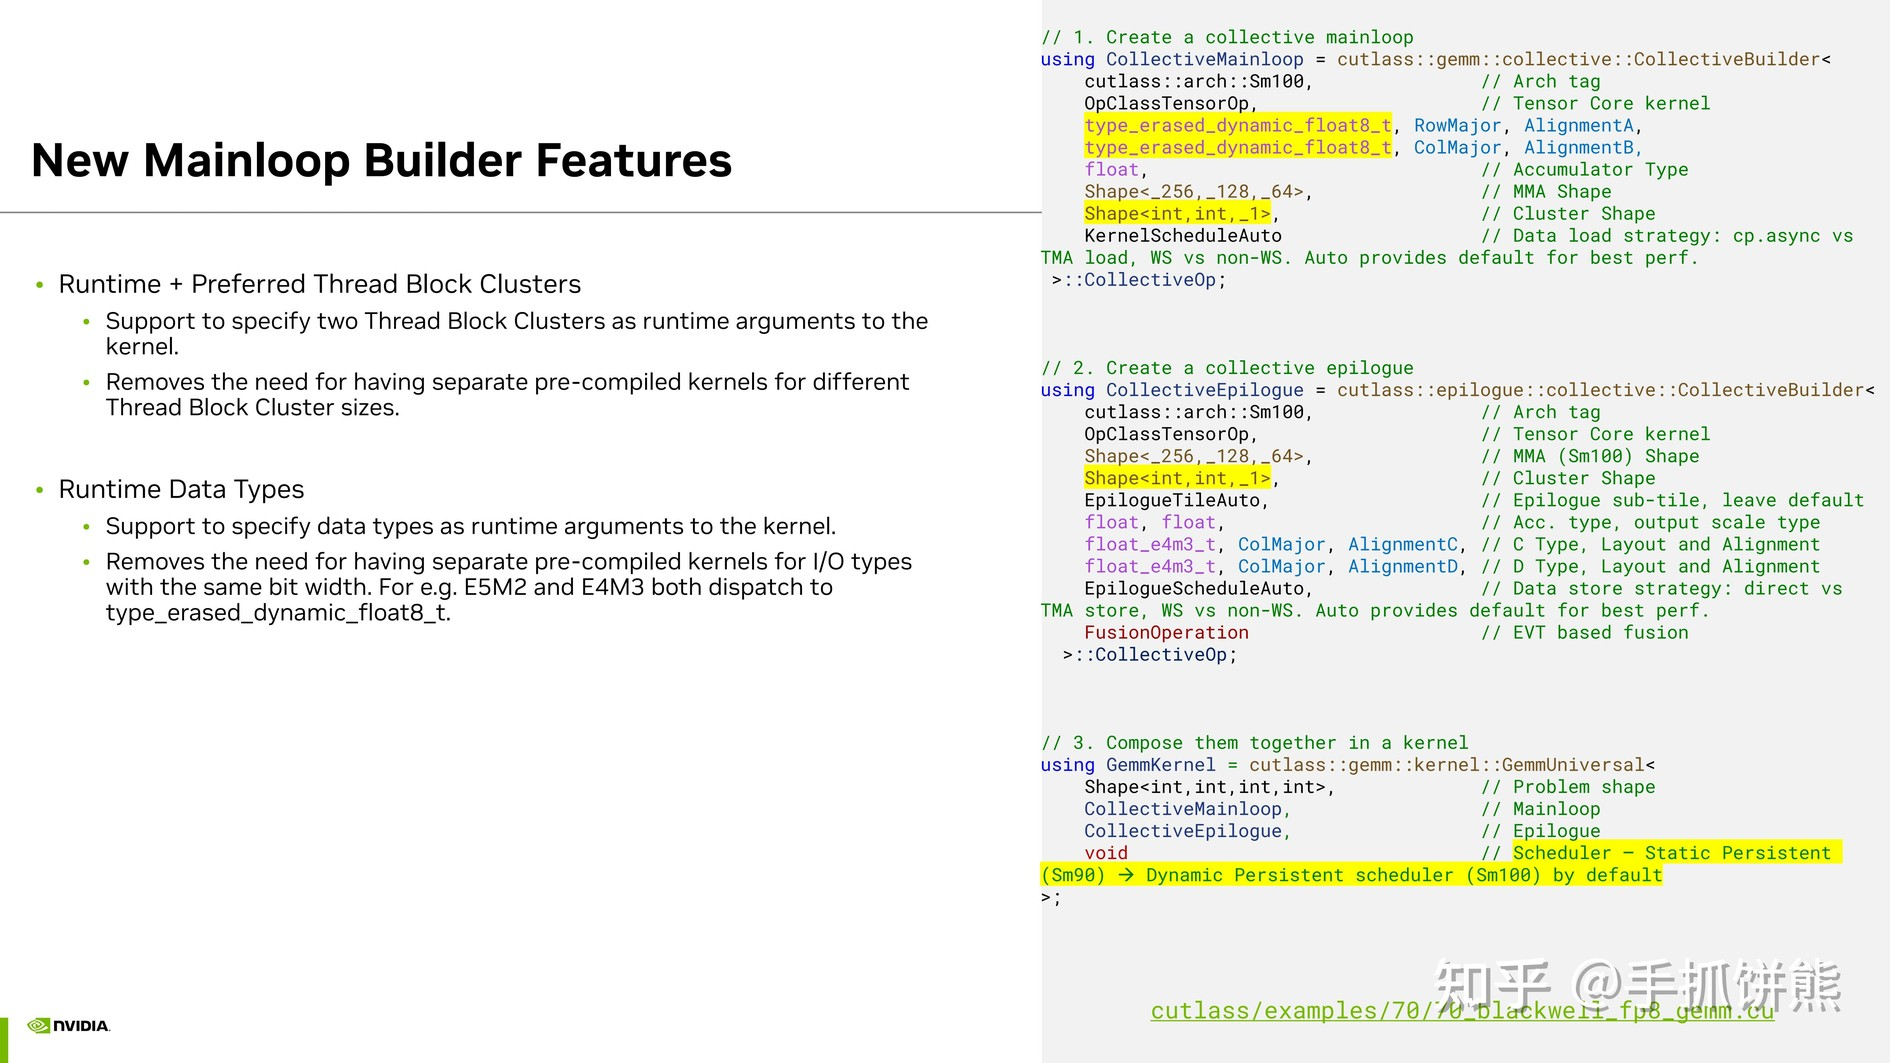
\includegraphics[width=0.9\textwidth]{figures/zhaoshangchun-01-tensor-core-programming/fig-62.jpg}
\end{figure}

本页揭示了 CUTLASS 4.0 在内核\textbf{灵活性和可组合性}方面的两项重大革新，旨在解决大规模模型部署中的一个核心痛点：内核编译爆炸 (kernel compilation explosion)。过去，不同的数据类型、线程块集群尺寸，甚至不同的后处理融合操作，都可能需要编译一个独立的内核版本，导致最终的二进制文件异常臃肿，增加了编译时间和部署管理的复杂性。

第一项革新是\textbf{将 Mainloop 与 Epilogue 分离并独立构建}。如代码所示，除了 \texttt{Collective\allowbreak{}Mainloop}，现在还有一个 \texttt{Collective\allowbreak{}Epilogue}，它专门负责 GEMM 计算完成后的处理阶段，包括数据写回、与激活函数（如 Re\allowbreak{}LU）或残差连接等操作的融合（Fusion）。这两者可以独立配置，最后在 \texttt{Gemm\allowbreak{}Universal} 内核模板中像积木一样“组装”起来。这种解耦设计极大地提升了代码的复用性和模块化程度。例如，同一个高性能的 \texttt{mainloop} 可以与十几种不同的 \texttt{epilogue} 自由组合，以应对各种复杂的融合需求，而无需为每种组合都重写一遍 \texttt{mainloop} 逻辑。

第二项，也是更具突破性的革新，是\textbf{引入了运行时配置能力}。幻灯片下半部分重点介绍了两个特性：\textbf{运行时线程块集群 (Runtime ... Thread Block Clusters)} 和 \textbf{运行时数据类型 (Runtime Data Types)}。前者意味着开发者不再需要在编译时写死 \texttt{Cluster Shape}，而是可以将其作为内核启动的运行时参数来传递。GPU 驱动和 CUTLASS 运行时将动态调整调度策略以适应传入的集群尺寸。这避免了为几种常见的 Cluster 尺寸（如 2x2, 4x2 等）预编译多个内核版本的窘境。后者则更进一步，通过 \texttt{t\allowbreak{}y\allowbreak{}p\allowbreak{}e\allowbreak{}\_\allowbreak{}e\allowbreak{}r\allowbreak{}a\allowbreak{}s\allowbreak{}e\allowbreak{}d\allowbreak{}\_\allowbreak{}d\allowbreak{}y\allowbreak{}n\allowbreak{}a\allowbreak{}m\allowbreak{}i\allowbreak{}c\allowbreak{}\_\allowbreak{}f\allowbreak{}l\allowbreak{}o\allowbreak{}a\allowbreak{}t\allowbreak{}8\allowbreak{}\_\allowbreak{}t} 这样的“类型擦除”技术，允许\textbf{用一个编译好的内核实例来处理所有位宽相同的 8-bit 浮点类型}（例如 E4\allowbreak{}M3 和 E5\allowbreak{}M2）。内核在运行时检查输入张量附带的元数据，动态地分发到正确的处理路径。这对大模型服务尤其重要，因为模型中的权重和激活可能使用不同的 FP8 变体，现在可以用一个统一的内核来高效处理，极大地简化了推理引擎的实现和部署。

\textbf{第 64 页：CUTLASS Kernel Example 组合}

\begin{figure}[H]\centering
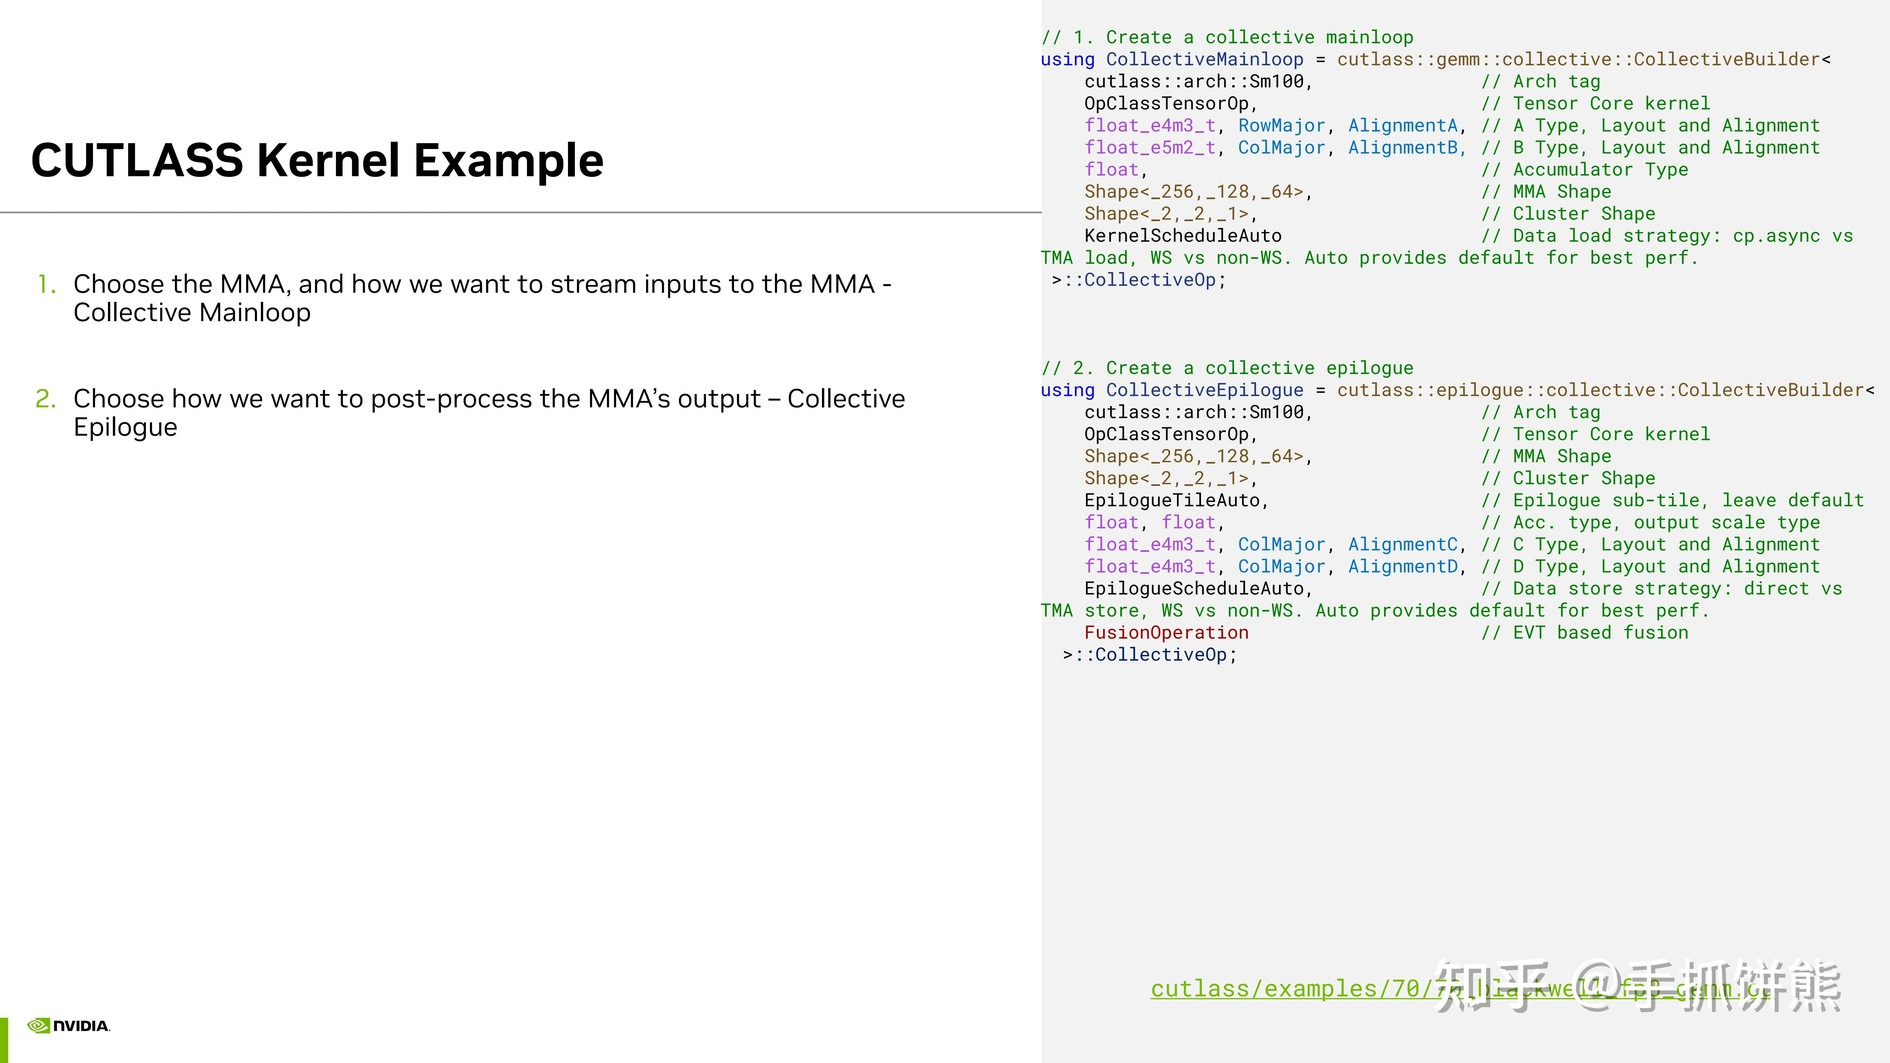
\includegraphics[width=0.9\textwidth]{figures/zhaoshangchun-01-tensor-core-programming/fig-63.jpg}
\end{figure}

这一页将定义 \texttt{Collective\allowbreak{}Mainloop} 和 \texttt{Collective\allowbreak{}Epilogue} 的代码并列展示，再次强调了 CUTLASS 的模块化和组合式思想。定义一个高性能 GEMM 内核的过程，被清晰地分解为两个独立的步骤：定义计算主循环，和定义后处理与写回。

这种解耦的设计带来了极大的灵活性。开发者可以独立地替换 Mainloop 或 Epilogue 的实现，例如，在同一个 Mainloop 的基础上，尝试不同的 Epilogue 融合策略（如 Re\allowbreak{}LU、GELU 等），或者在同一个 Epilogue 的基础上，试验不同的 Mainloop 调度策略。这种正交组合的能力，是 CUTLASS 成为一个强大而灵活的算子研发框架的基石。

\textbf{第 65 页：Collective Epilogue 与 Builder}

\begin{figure}[H]\centering
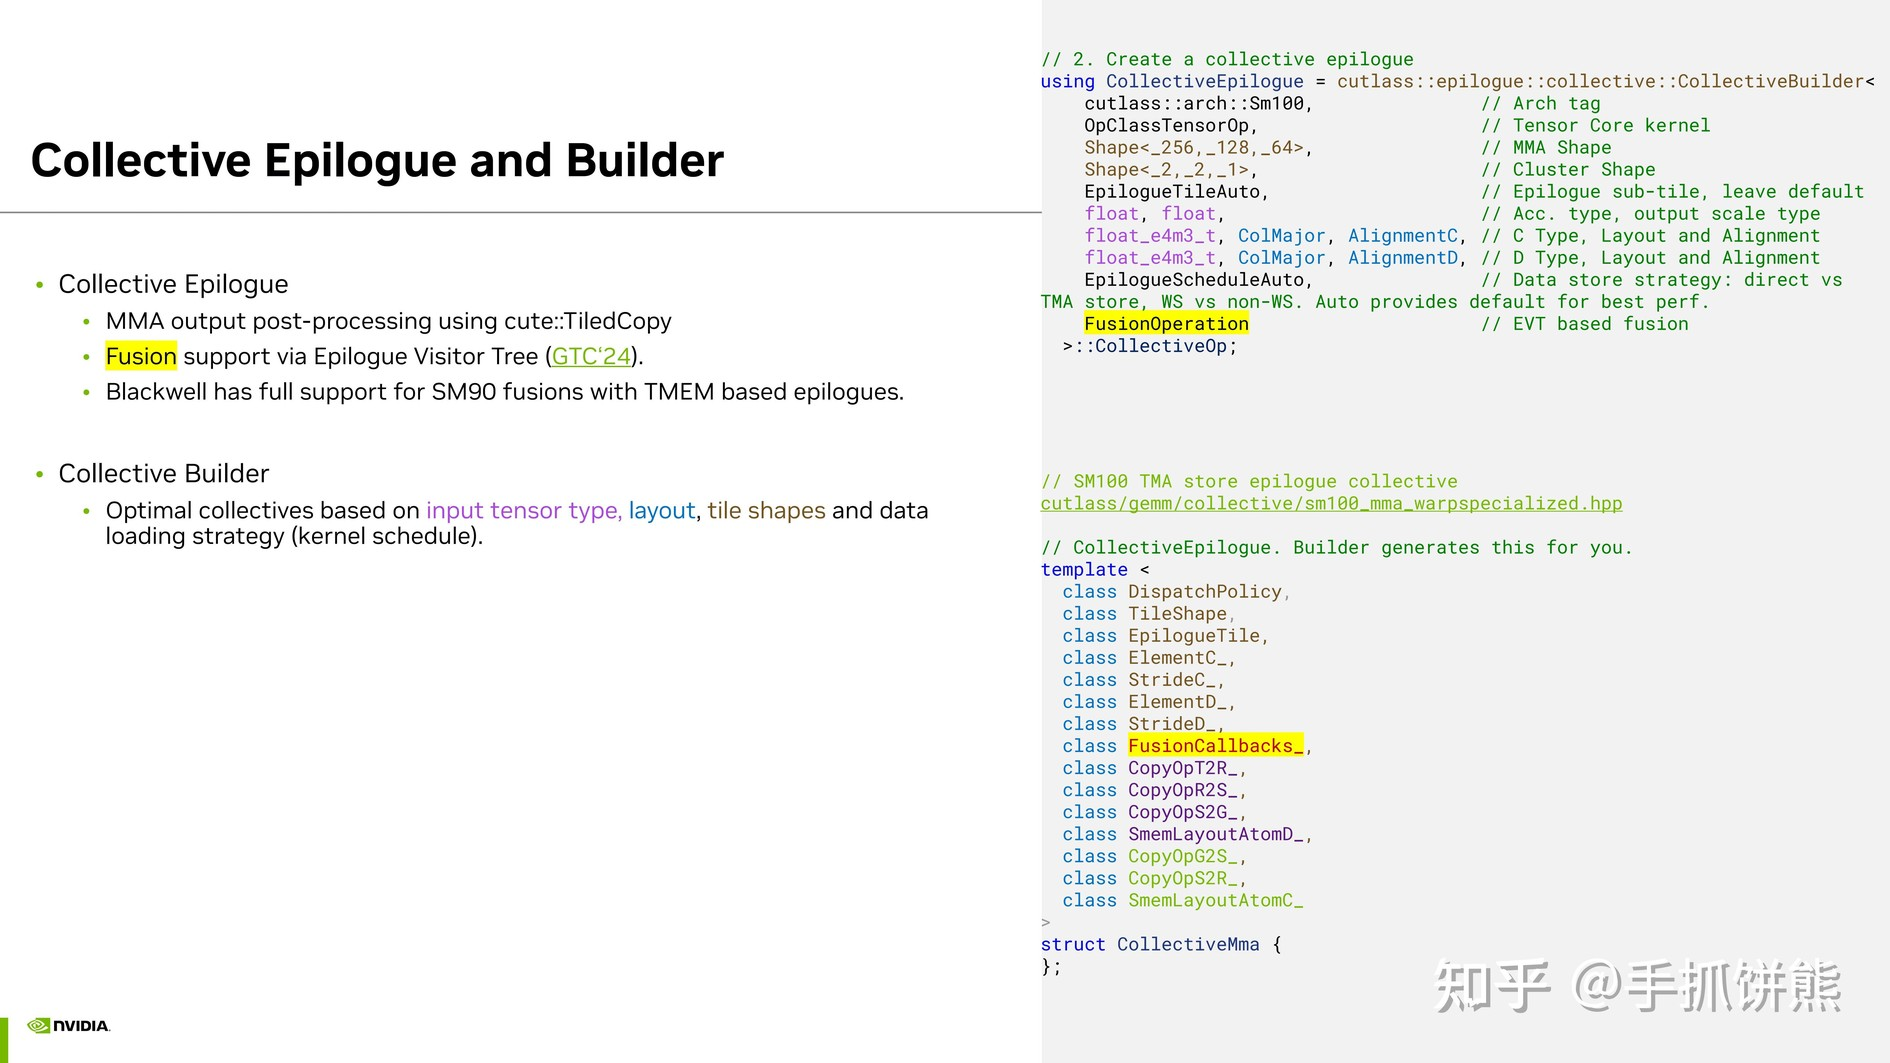
\includegraphics[width=0.9\textwidth]{figures/zhaoshangchun-01-tensor-core-programming/fig-64.jpg}
\end{figure}

这一页介绍了与 \texttt{Collective\allowbreak{}Mainloop} 配套的 \texttt{Collective\allowbreak{}Epilogue}，它是 CUTLASS 4.0 中 GEMM 计算流程的后半部分，负责处理 Tensor Core 计算完成后的数据后处理与写回。\texttt{Collective\allowbreak{}Epilogue} 的设计同样遵循了 \texttt{Collective\allowbreak{}Builder} 的思想，即通过一套高层抽象来自动生成针对 Blackwell 架构优化的 Epilogue（收尾）部分代码。

\texttt{Collective\allowbreak{}Epilogue} 的核心职责包括：\textbf{数据类型转换、可选的 Element-wise 融合操作、以及最终结果的写回}。在 Blackwell 架构上，MMA (Matrix Multiply-Accumulate) 的累加结果通常存放在寄存器（RMEM）或线程块内存（TMEM）中。Epilogue 需要将这些高精度的累加值（如 FP32）转换为目标输出格式（如 FP8），并应用可能的融合操作，比如 Bias、Re\allowbreak{}LU 激活或者与其他张量的逐元素相加。这张 PPT 特别强调了 \textbf{Fusion support via Epilogue Visitor Tree (EVT)}，这是从 Hopper 架构延续并强化的特性。EVT 允许开发者以一种可组合、可扩展的方式定义复杂的融合操作链，而无需手动编写繁琐的 C++ 模板代码。Blackwell 架构完全兼容基于 TMEM 的 SM90（Hopper）融合模式，保证了代码的可移植性。

实现原理：\texttt{Collective\allowbreak{}Epilogue} Builder 参数解析 与 \texttt{Collective\allowbreak{}Mainloop} 类似，\texttt{Collective\allowbreak{}Epilogue} 也是通过 \texttt{Collective\allowbreak{}Builder} 模板类来配置的。其关键模板参数包括：

\begin{itemize}
\item \textbf{\texttt{cutlass::\allowbreak{}arch::\allowbreak{}Sm100}}：架构标记，确保生成的代码适配 Blackwell 的新特性，例如 TMA（Tensor Memory Accelerator）用于数据存储。
\item \textbf{\texttt{Shape} (MMA Shape \& Cluster Shape)}：与 Mainloop 保持一致的 Tile 形状和 Cluster 形状，以确保数据在 Mainloop 和 Epilogue 之间正确传递。
\item \textbf{\texttt{C Type} /\allowbreak{} \texttt{D Type}}：分别定义了输入/\allowbreak{}输出张量 C 和最终输出张量 D 的数据类型、布局和对齐方式。这使得 Epilogue 可以处理 \texttt{D\allowbreak{} \allowbreak{}=\allowbreak{} \allowbreak{}a\allowbreak{}l\allowbreak{}p\allowbreak{}h\allowbreak{}a\allowbreak{} \allowbreak{}*\allowbreak{} \allowbreak{}A\allowbreak{} \allowbreak{}*\allowbreak{} \allowbreak{}B\allowbreak{} \allowbreak{}+\allowbreak{} \allowbreak{}b\allowbreak{}e\allowbreak{}t\allowbreak{}a\allowbreak{} \allowbreak{}*\allowbreak{} \allowbreak{}C} 这样的通用 GEMM 形式。
\item \textbf{\texttt{Epilogue\allowbreak{}Schedule\allowbreak{}Auto}}：这是一个关键的自动化策略。它让 CUTLASS 根据上下文自动选择最优的数据写回方式，例如是直接从寄存器写回（Direct Store），还是利用 TMA 进行异步存储。这大大降低了手动调优的复杂度。对于开发者而言，只需关注逻辑，而将硬件相关的调度细节交给库来处理。
\item \textbf{\texttt{Fusion\allowbreak{}Operation}}：这是一个占位符，用于传入通过 EVT 定义的融合操作。这使得 \texttt{Collective\allowbreak{}Epilogue} 成为一个高度可定制的计算节点。
\end{itemize}

\texttt{Collective\allowbreak{}Epilogue} 和 \texttt{Builder} 的设计对工程实践带来了巨大影响。首先，\textbf{它极大地简化了高性能融合算子的开发}。在过去，要实现一个高效的 \texttt{GEMM + Bias + Re\allowbreak{}LU} 内核，开发者需要深入了解 PTX 指令、共享内存布局和复杂的同步逻辑。现在，通过 \texttt{Collective\allowbreak{}Builder} 和 EVT，开发者可以像搭积木一样组合这些操作，代码更清晰，也更易于维护。其次，\textbf{性能得到了保证}。\texttt{Epilogue\allowbreak{}Schedule\allowbreak{}Auto} 和针对 \texttt{Sm100} 的优化确保了生成的代码能够充分利用 Blackwell 的硬件特性，如 TMA Store，以隐藏数据写回的延迟，从而提升整体的计算吞吐。最后，它\textbf{增强了代码的可复用性}。一旦定义好了一个 \texttt{Collective\allowbreak{}Epilogue}，它就可以在不同的 GEMM 内核中重复使用，只需调整模板参数即可适应不同的数据类型或融合需求。这与现代软件工程中“高内聚、低耦合”的设计原则不谋而合。

\textbf{第 66 页：为 Blackwell 预调优的新 Collective Epilogues}

\begin{figure}[H]\centering
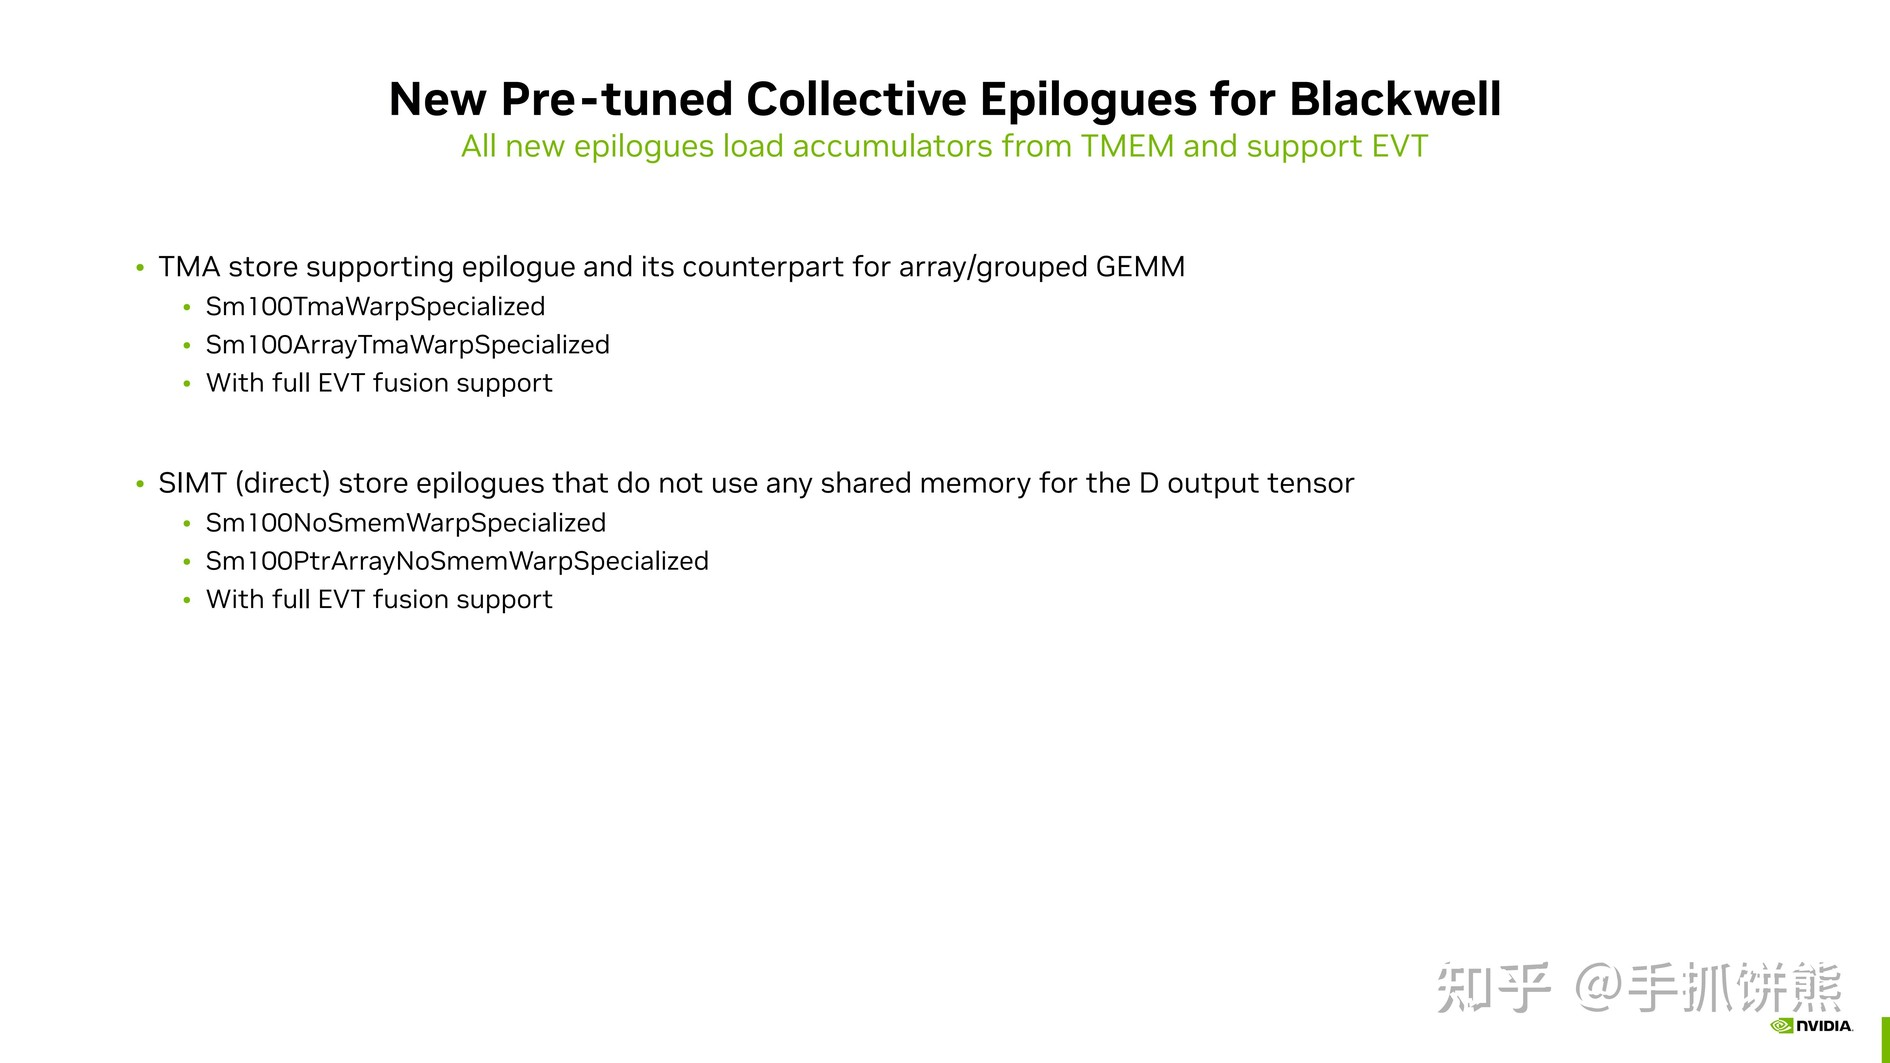
\includegraphics[width=0.9\textwidth]{figures/zhaoshangchun-01-tensor-core-programming/fig-65.jpg}
\end{figure}

这一页具体列出了 CUTLASS 为 Blackwell 架构预先调整和优化的几种 \texttt{Collective Epilogue} 实现。这些实现是 \texttt{C\allowbreak{}o\allowbreak{}l\allowbreak{}l\allowbreak{}e\allowbreak{}c\allowbreak{}t\allowbreak{}i\allowbreak{}v\allowbreak{}e\allowbreak{}E\allowbreak{}p\allowbreak{}i\allowbreak{}l\allowbreak{}o\allowbreak{}g\allowbreak{}u\allowbreak{}e\allowbreak{}:\allowbreak{}:\allowbreak{}B\allowbreak{}u\allowbreak{}i\allowbreak{}l\allowbreak{}d\allowbreak{}e\allowbreak{}r} 在 \texttt{Epilogue\allowbreak{}Schedule\allowbreak{}Auto} 模式下可能选择的具体策略，它们都支持 Epilogue Visitor Tree (EVT) 融合，并针对 Blackwell 的内存子系统进行了深度优化。

此页的核心在于区分两种主要的 Epilogue 写回策略：\textbf{TMA Store} 和 \textbf{SIMT (Direct) Store}。

\begin{itemize}
\item \textbf{\texttt{Sm100\allowbreak{}Tma\allowbreak{}Warp\allowbreak{}Specialized} 和 \texttt{S\allowbreak{}m\allowbreak{}1\allowbreak{}0\allowbreak{}0\allowbreak{}A\allowbreak{}r\allowbreak{}r\allowbreak{}a\allowbreak{}y\allowbreak{}T\allowbreak{}m\allowbreak{}a\allowbreak{}W\allowbreak{}a\allowbreak{}r\allowbreak{}p\allowbreak{}S\allowbreak{}p\allowbreak{}e\allowbreak{}c\allowbreak{}i\allowbreak{}a\allowbreak{}l\allowbreak{}i\allowbreak{}z\allowbreak{}e\allowbreak{}d}}：这两种 Epilogue 使用 Blackwell 引入的 \textbf{Tensor Memory Accelerator (TMA)} 来执行异步数据写回。TMA 是一个硬件加速单元，能够高效地处理 Global Memory 与 Shared Memory 之间的大块、多维张量数据传输。在 Epilogue 阶段使用 TMA，意味着可以将计算核心（Tensor Core）从繁琐的地址计算和数据写回指令中解放出来，让硬件去处理这些任务。这种方式特别适合处理大的输出 Tile，能够有效隐藏访存延迟，提升性能。\texttt{Array} 版本则专为 Grouped GEMM 设计，可以一次性处理多个 GEMM 的输出。
\item \textbf{\texttt{S\allowbreak{}m\allowbreak{}1\allowbreak{}0\allowbreak{}0\allowbreak{}N\allowbreak{}o\allowbreak{}S\allowbreak{}m\allowbreak{}e\allowbreak{}m\allowbreak{}W\allowbreak{}a\allowbreak{}r\allowbreak{}p\allowbreak{}S\allowbreak{}p\allowbreak{}e\allowbreak{}c\allowbreak{}i\allowbreak{}a\allowbreak{}l\allowbreak{}i\allowbreak{}z\allowbreak{}e\allowbreak{}d} 和 \texttt{S\allowbreak{}m\allowbreak{}1\allowbreak{}0\allowbreak{}0\allowbreak{}P\allowbreak{}t\allowbreak{}r\allowbreak{}A\allowbreak{}r\allowbreak{}r\allowbreak{}a\allowbreak{}y\allowbreak{}N\allowbreak{}o\allowbreak{}S\allowbreak{}m\allowbreak{}e\allowbreak{}m\allowbreak{}W\allowbreak{}a\allowbreak{}r\allowbreak{}p\allowbreak{}S\allowbreak{}p\allowbreak{}e\allowbreak{}c\allowbreak{}i\allowbreak{}a\allowbreak{}l\allowbreak{}i\allowbreak{}z\allowbreak{}e\allowbreak{}d}}：这两种 Epilogue 采用了更直接的写回方式，通常称为 “SIMT Store” 或 “Direct Store”。它们\textbf{不使用共享内存（Shared Memory）作为 D 矩阵输出的中转}，而是由 SIMT 核心（CUDA Core）直接将计算结果从寄存器写回到 Global Memory。这种策略的优势在于节省了共享内存资源，对于某些共享内存非常紧张的内核，或者输出 Tile 较小、TMA 开销不划算的场景，这种直接写回的方式可能效率更高。
\end{itemize}

所有这些新的 Epilogue 都采用了 \textbf{Warp-Specialized (WS)} 设计。在 WS 架构中，一个 Thread Block 内的 Warps 会被分成不同的角色。一些 Warps 专注于执行 MMA 计算，而另一些 Warps 则专门负责 Epilogue 的数据处理和写回。这种分工协作的模式，结合异步内存操作（如 TMA），可以构建出更深、更高效的软件流水线（Pipeline），使得计算和访存能够最大程度地重叠。例如，当 Epilogue Warps 正在处理上一个计算阶段的结果时，MMA Warps 已经开始计算下一个 Tile，从而掩盖了 Epilogue 的执行开销。

对于 CUDA 工程师来说，理解这两种 Epilogue 的差异至关重要。

\begin{itemize}
\item \textbf{性能优先，选择 TMA Store}：在大多数情况下，特别是对于大规模的 GEMM 计算，\texttt{Sm100\allowbreak{}Tma\allowbreak{}Warp\allowbreak{}Specialized} 是首选。它能最大化地利用 Blackwell 的硬件能力，获得最佳性能。当 \texttt{Epilogue\allowbreak{}Schedule\allowbreak{}Auto} 被启用时，CUTLASS 通常会优先选择它。
\item \textbf{资源受限或小矩阵，考虑 Direct Store}：如果你的内核非常复杂，占用了大量共享内存，导致 Occupancy 下降，那么可以尝试使用 \texttt{S\allowbreak{}m\allowbreak{}1\allowbreak{}0\allowbreak{}0\allowbreak{}N\allowbreak{}o\allowbreak{}S\allowbreak{}m\allowbreak{}e\allowbreak{}m\allowbreak{}W\allowbreak{}a\allowbreak{}r\allowbreak{}p\allowbreak{}S\allowbreak{}p\allowbreak{}e\allowbreak{}c\allowbreak{}i\allowbreak{}a\allowbreak{}l\allowbreak{}i\allowbreak{}z\allowbreak{}e\allowbreak{}d}。通过省去 Epilogue 使用的共享内存，可以为 Mainloop 阶段腾出更多资源，或者支持更大的 Thread Block 配置。此外，对于那些输出矩阵非常小、形状奇特的 GEMM，TMA 的设置开销可能超过其带来的收益，此时 Direct Store 可能是更明智的选择。
\item \textbf{Grouped GEMM 场景}：当你需要一次性处理大量小 GEMM 时（例如在 Mo\allowbreak{}E 模型中），\texttt{Array} 版本的 Epilogue (\texttt{S\allowbreak{}m\allowbreak{}1\allowbreak{}0\allowbreak{}0\allowbreak{}A\allowbreak{}r\allowbreak{}r\allowbreak{}a\allowbreak{}y\allowbreak{}T\allowbreak{}m\allowbreak{}a\allowbreak{}W\allowbreak{}a\allowbreak{}r\allowbreak{}p\allowbreak{}S\allowbreak{}p\allowbreak{}e\allowbreak{}c\allowbreak{}i\allowbreak{}a\allowbreak{}l\allowbreak{}i\allowbreak{}z\allowbreak{}e\allowbreak{}d} 或 \texttt{S\allowbreak{}m\allowbreak{}1\allowbreak{}0\allowbreak{}0\allowbreak{}P\allowbreak{}t\allowbreak{}r\allowbreak{}A\allowbreak{}r\allowbreak{}r\allowbreak{}a\allowbreak{}y\allowbreak{}N\allowbreak{}o\allowbreak{}S\allowbreak{}m\allowbreak{}e\allowbreak{}m\allowbreak{}W\allowbreak{}a\allowbreak{}r\allowbreak{}p\allowbreak{}S\allowbreak{}p\allowbreak{}e\allowbreak{}c\allowbreak{}i\allowbreak{}a\allowbreak{}l\allowbreak{}i\allowbreak{}z\allowbreak{}e\allowbreak{}d}) 是不二之选。它们通过批处理减少了 Kernel Launch 的开销，并能更有效地利用 GPU 资源。
\end{itemize}

总而言之，CUTLASS 提供的这些预调优 Epilogue 给了开发者一个清晰的选择光谱。通过 \texttt{Collective\allowbreak{}Builder}，开发者可以轻松地在这些策略间切换，快速找到最适合自己应用场景的方案，而无需从头实现复杂的硬件适配逻辑。

\textbf{第 67 页：CUTLASS Kernel 示例：组合 Mainloop 与 Epilogue}

\begin{figure}[H]\centering
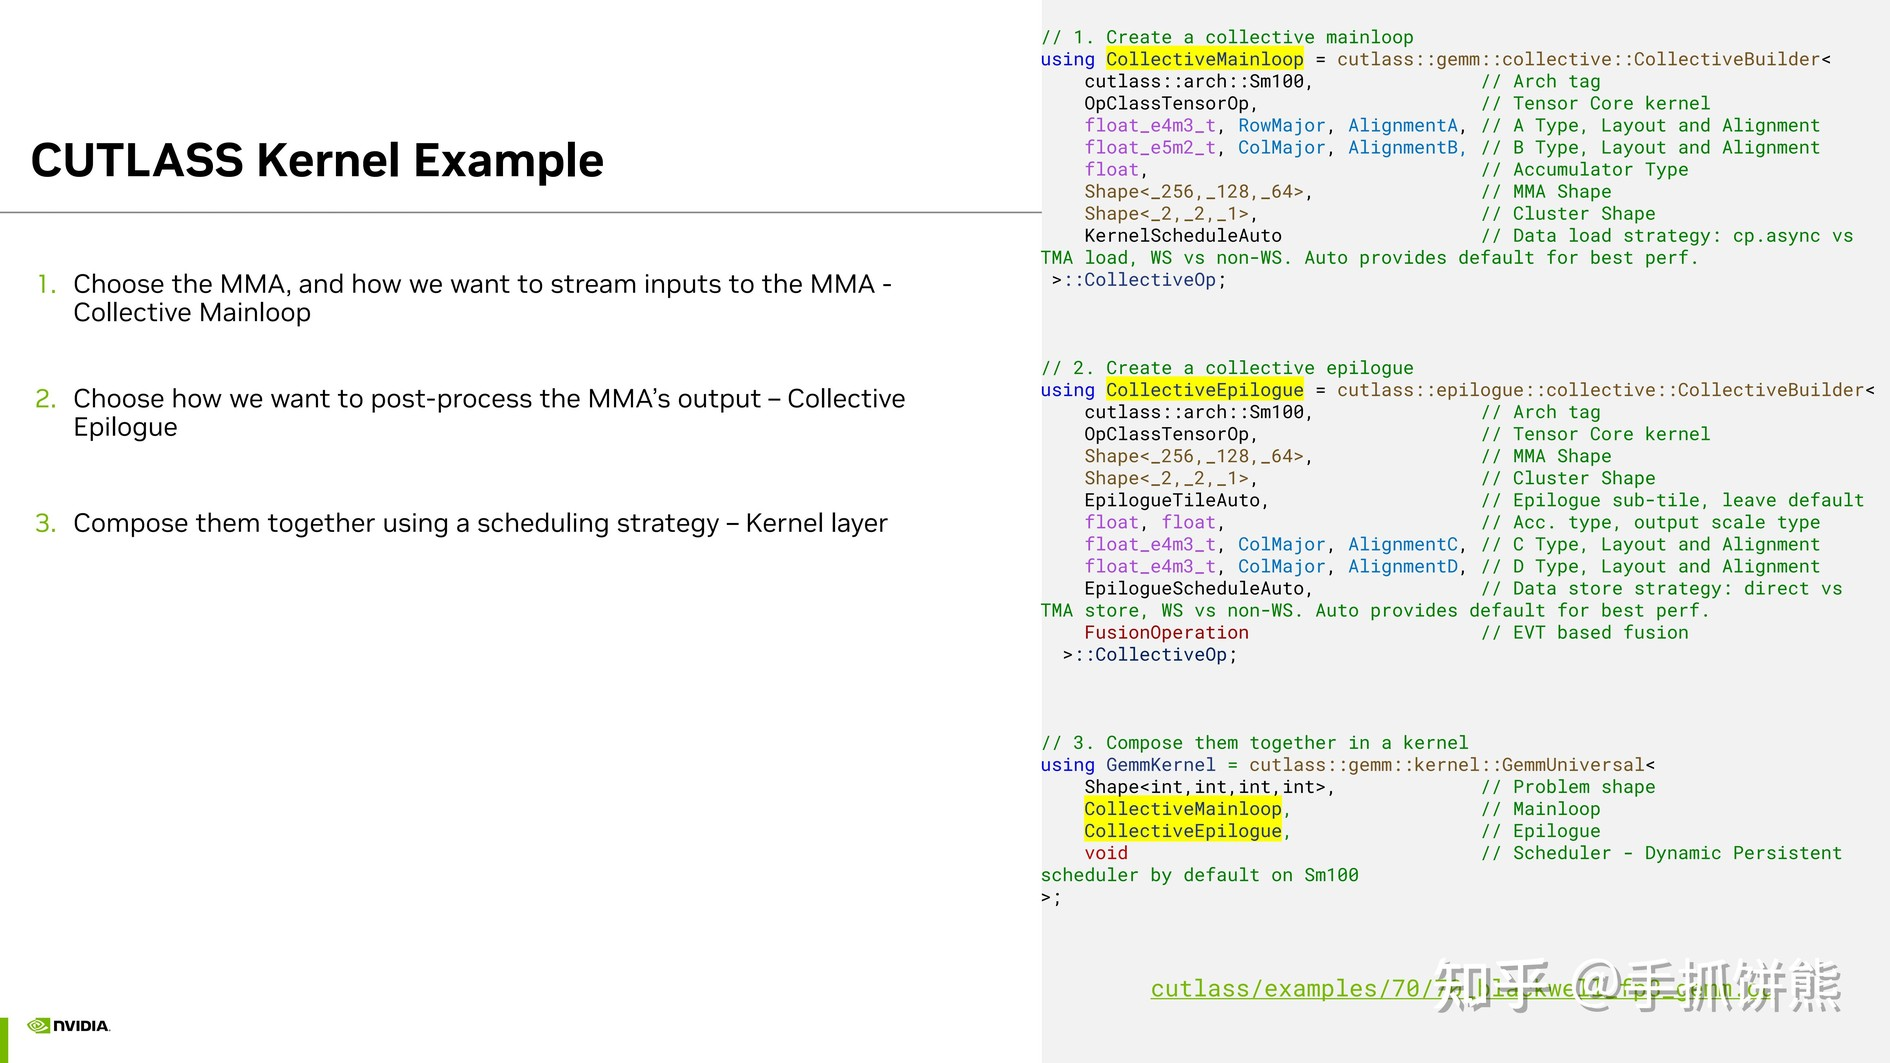
\includegraphics[width=0.9\textwidth]{figures/zhaoshangchun-01-tensor-core-programming/fig-66.jpg}
\end{figure}

这一页通过一个完整的代码示例，展示了 CUTLASS 4.0 中构建一个 GEMM Kernel 的“三步走”流程。它清晰地演示了如何将前面介绍的 \texttt{Collective\allowbreak{}Mainloop} 和 \texttt{Collective\allowbreak{}Epilogue} 像积木一样拼装起来，最终形成一个可执行的、高度优化的 \texttt{Gemm\allowbreak{}Universal} 内核。

构建一个完整的 GEMM 内核被分解为三个独立的、正交的步骤：

\begin{enumerate}
\item \textbf{创建 \texttt{Collective\allowbreak{}Mainloop}}：这一步定义了 GEMM 的核心计算部分，即 K 维度上的循环。如前所述，它负责数据的加载（A 和 B 矩阵）、软件流水线的调度以及 MMA 计算的执行。\texttt{Collective\allowbreak{}Builder} 在这里扮演了关键角色，它根据所选的架构、数据类型和 Tile 形状，自动生成最优化的 Mainloop 实现。
\item \textbf{创建 \texttt{Collective\allowbreak{}Epilogue}}：这一步定义了 GEMM 的收尾部分。它接收 Mainloop 计算出的累加值，并执行数据后处理，如类型转换、融合操作（Bias、Re\allowbreak{}LU 等）以及最终结果的写回。
\item \textbf{组合成 \texttt{Gemm\allowbreak{}Universal} Kernel}：最后一步是将 \texttt{Collective\allowbreak{}Mainloop} 和 \texttt{Collective\allowbreak{}Epilogue} 传递给 \texttt{c\allowbreak{}u\allowbreak{}t\allowbreak{}l\allowbreak{}a\allowbreak{}s\allowbreak{}s\allowbreak{}:\allowbreak{}:\allowbreak{}g\allowbreak{}e\allowbreak{}m\allowbreak{}m\allowbreak{}:\allowbreak{}:\allowbreak{}k\allowbreak{}e\allowbreak{}r\allowbreak{}n\allowbreak{}e\allowbreak{}l\allowbreak{}:\allowbreak{}:\allowbreak{}G\allowbreak{}e\allowbreak{}m\allowbreak{}m\allowbreak{}U\allowbreak{}n\allowbreak{}i\allowbreak{}v\allowbreak{}e\allowbreak{}r\allowbreak{}s\allowbreak{}a\allowbreak{}l} 模板。这个 \texttt{Gemm\allowbreak{}Universal} 类是一个高阶组件，它负责处理线程块（Thread Block）的调度、网格（Grid）的划分以及内核的启动和参数传递。本质上，它是一个框架，将计算的核心逻辑（Mainloop）和后处理逻辑（Epilogue）粘合在一起。
\end{enumerate}

\texttt{Gemm\allowbreak{}Universal} 的关键模板参数包括：

\begin{itemize}
\item \textbf{\texttt{Problem Shape}}：定义了输入矩阵的维度（M, N, K, L - L 用于 Grouped GEMM）。
\item \textbf{\texttt{Collective\allowbreak{}Mainloop}}：传入第一步中定义的 Mainloop 类型。
\item \textbf{\texttt{Collective\allowbreak{}Epilogue}}：传入第二步中定义的 Epilogue 类型。
\item \textbf{\texttt{Scheduler}}：这是一个非常重要的参数，它定义了\textbf{线程块调度策略}。在此示例中，它被设置为 \texttt{void}，表示使用 CUTLASS 在 SM100 上的\textbf{默认调度器}，即 \textbf{Dynamic Persistent Scheduler}。这个调度器是一种动态负载均衡策略，特别适合在 GPU 上处理不规则或大小不一的计算任务，能有效提升硬件利用率。
\end{itemize}

这种模块化的设计哲学对 CUDA 开发产生了深远影响。它允许开发者将关注点从繁琐的底层实现细节（“如何做”）转移到更高层次的算法策略（“做什么”）。

\begin{itemize}
\item \textbf{解耦与复用}：Mainloop 和 Epilogue 的解耦，使得两者可以独立演进和优化。例如，你可以为同一个 Mainloop 搭配不同的 Epilogue（一个带 Bias，一个不带），或者为同一个 Epilogue 搭配不同的 Mainloop（一个用 TMA，一个用 \texttt{cp.\allowbreak{}async}）。这种灵活性和可复用性是传统手工编写内核难以企及的。
\item \textbf{快速迭代与实验}：当需要测试不同策略时，开发者不再需要重写整个内核。只需更改 \texttt{Collective\allowbreak{}Builder} 的模板参数，或者在 \texttt{Gemm\allowbreak{}Universal} 中替换一个组件，就可以快速编译和测试一个新的内核变体。这大大缩短了性能调优的周期。
\item \textbf{降低入门门槛}：对于初学者或非 GPU 专家，他们无需理解 TMA 的所有细节或 \texttt{mbarrier} 的复杂用法，就可以通过这套高层抽象构建出性能卓越的内核。他们只需关心自己的算法逻辑，并将其表达为 CUTLASS 的组件组合。如 \texttt{70\_\allowbreak{}blackwell\_\allowbreak{}fp8\_\allowbreak{}gemm.\allowbreak{}cu} 示例所示，一个复杂的 FP8 GEMM 内核可以被浓缩为几行清晰的 C++ \texttt{using} 声明，极大地提升了代码的可读性和可维护性。
\end{itemize}

\textbf{第 68 页：深入 CUTLASS Kernel Layer}

\begin{figure}[H]\centering
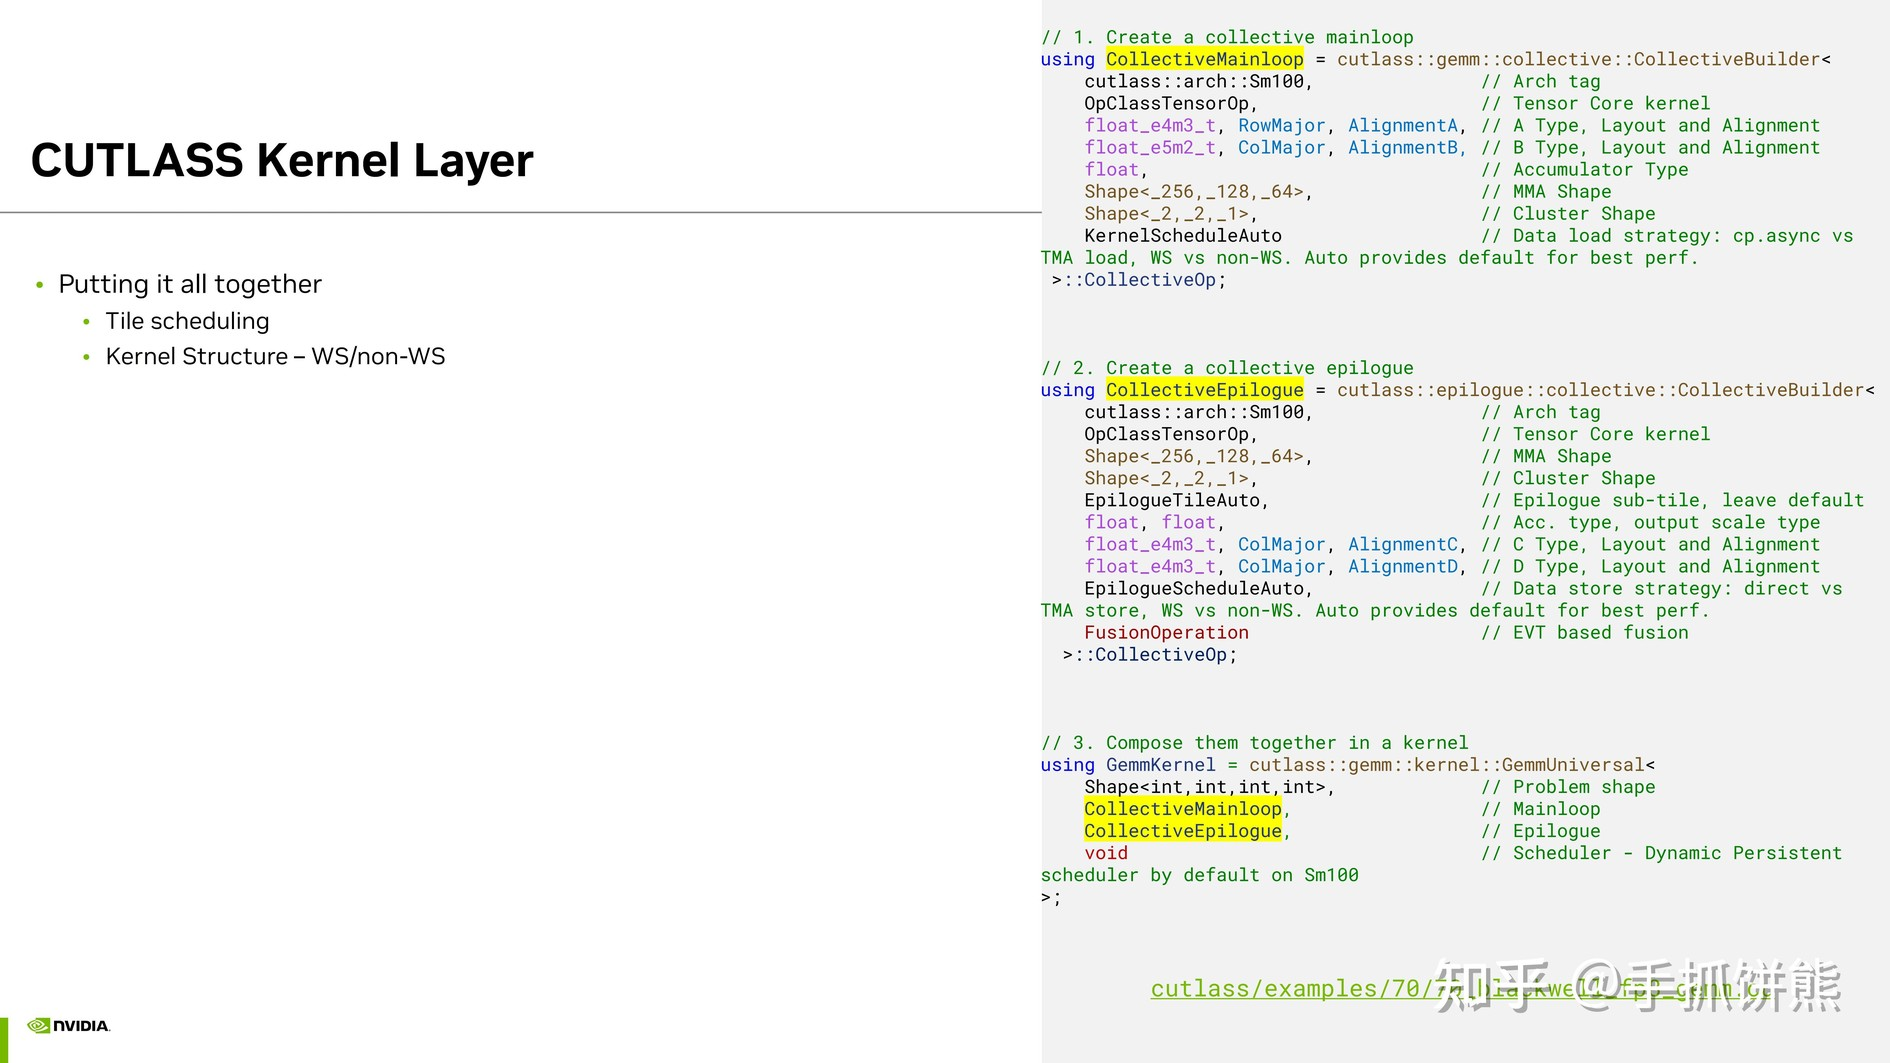
\includegraphics[width=0.9\textwidth]{figures/zhaoshangchun-01-tensor-core-programming/fig-67.jpg}
\end{figure}

这一页可以看作是第 67 页的进一步阐述，它重申了 \texttt{CUTLASS Kernel Layer} 的核心思想：\textbf{将所有部分组合在一起（Putting it all together）}。它强调了 Kernel Layer 的两个主要职责：\textbf{Tile 调度（Tile scheduling）} 和 \textbf{内核结构（Kernel Structure）} 的管理。

\texttt{Gemm\allowbreak{}Universal} 作为 Kernel Layer 的核心，其设计精髓在于将“计算任务的划分与分发”（调度）和“单个计算任务的具体执行方式”（结构）分离开来。

\begin{itemize}
\item \textbf{Tile 调度}：这是指如何将整个 GEMM 问题（一个巨大的 M x N 矩阵）分解成许多个小的 Tile，并将这些 Tile 分配给 GPU 上的线程块（Thread Blocks /\allowbreak{} CTAs）去处理。调度策略决定了哪个 CTA 计算哪个 Tile，以及计算的顺序。一个好的调度策略能够实现负载均衡，避免部分 SM 闲置，同时也能优化数据局部性，减少对 Global Memory 的访问。
\item \textbf{内核结构}：这是指单个线程块内部的工作方式。例如，是采用 Warp-Specialized（WS）还是非 WS 结构？软件流水线的深度是多少？共享内存如何划分？这些都属于内核结构的范畴。它决定了单个 CTA 执行其分配到的 Tile 的效率。
\end{itemize}

PPT 中再次高亮了 \texttt{Gemm\allowbreak{}Universal} 的第四个模板参数 \texttt{Scheduler}。当它被省略（或设为 \texttt{void}）时，CUTLASS 4.0 在 SM100 架构上会默认启用 \textbf{Dynamic Persistent Scheduler}

\begin{itemize}
\item \textbf{Persistent (持久化)}：这意味着一旦一个线程块被启动，它不会在完成一个 Tile 后就立即退出，而是会继续向调度器请求下一个 Tile 进行计算，直到所有 Tile 都被处理完毕。这种方式避免了反复启动和销毁线程块的开销，对于包含大量 Tile 的大矩阵尤其高效。
\item \textbf{Dynamic (动态)}：与静态调度（在编译时就确定好每个 CTA 的任务）不同，动态调度是在运行时进行的。每个持久化的 CTA 就像一个工作线程，完成任务后会去“任务队列”里领取新任务。这使得它能很好地适应不规则的矩阵尺寸和动态变化的工作负载，实现更好的负载均衡。Blackwell 架构中的 CLC（Compute-Local Cache，可能是某种用于快速同步或任务分发的硬件机制）可能为此提供了硬件层面的支持。
\end{itemize}

对于开发者而言，Kernel Layer 的设计意味着他们可以站在一个更高的维度上思考性能优化。

\begin{itemize}
\item \textbf{默认即最优（大部分情况）}：对于大多数标准的 GEMM 应用，直接使用 \texttt{Gemm\allowbreak{}Universal} 的默认配置（即 \texttt{D\allowbreak{}y\allowbreak{}n\allowbreak{}a\allowbreak{}m\allowbreak{}i\allowbreak{}c\allowbreak{} \allowbreak{}P\allowbreak{}e\allowbreak{}r\allowbreak{}s\allowbreak{}i\allowbreak{}s\allowbreak{}t\allowbreak{}e\allowbreak{}n\allowbreak{}t\allowbreak{} \allowbreak{}S\allowbreak{}c\allowbreak{}h\allowbreak{}e\allowbreak{}d\allowbreak{}u\allowbreak{}l\allowbreak{}e\allowbreak{}r}）就已经能获得非常接近最优的性能。这体现了 CUTLASS 的一个核心理念：将硬件的最佳实践封装到库中，让用户可以轻松受益。
\item \textbf{专注于“策略”而非“机制”}：开发者不再需要自己实现复杂的调度逻辑。他们可以将精力集中在更高层次的策略选择上，例如：我的应用场景是否适合 Stream-K？我的 Epilogue 是否需要特殊的融合逻辑？通过在 \texttt{Gemm\allowbreak{}Universal} 中插入不同的调度器或 Epilogue 组件，开发者可以快速验证这些策略的效果。
\item \textbf{提升代码的可读性和可维护性}：通过将调度逻辑从核心计算代码中剥离出来，整个内核的结构变得更加清晰。\texttt{Collective\allowbreak{}Mainloop} 和 \texttt{Collective\allowbreak{}Epilogue} 只关心数据处理的流程，而 \texttt{Gemm\allowbreak{}Universal} 和 \texttt{Scheduler} 则关心任务的组织和分发。这种关注点分离（Separation of Concerns）的设计使得代码更容易被理解和修改。
\end{itemize}

\textbf{第 69 页：Kernel Layer 的调度策略：Stream-K}

\begin{figure}[H]\centering
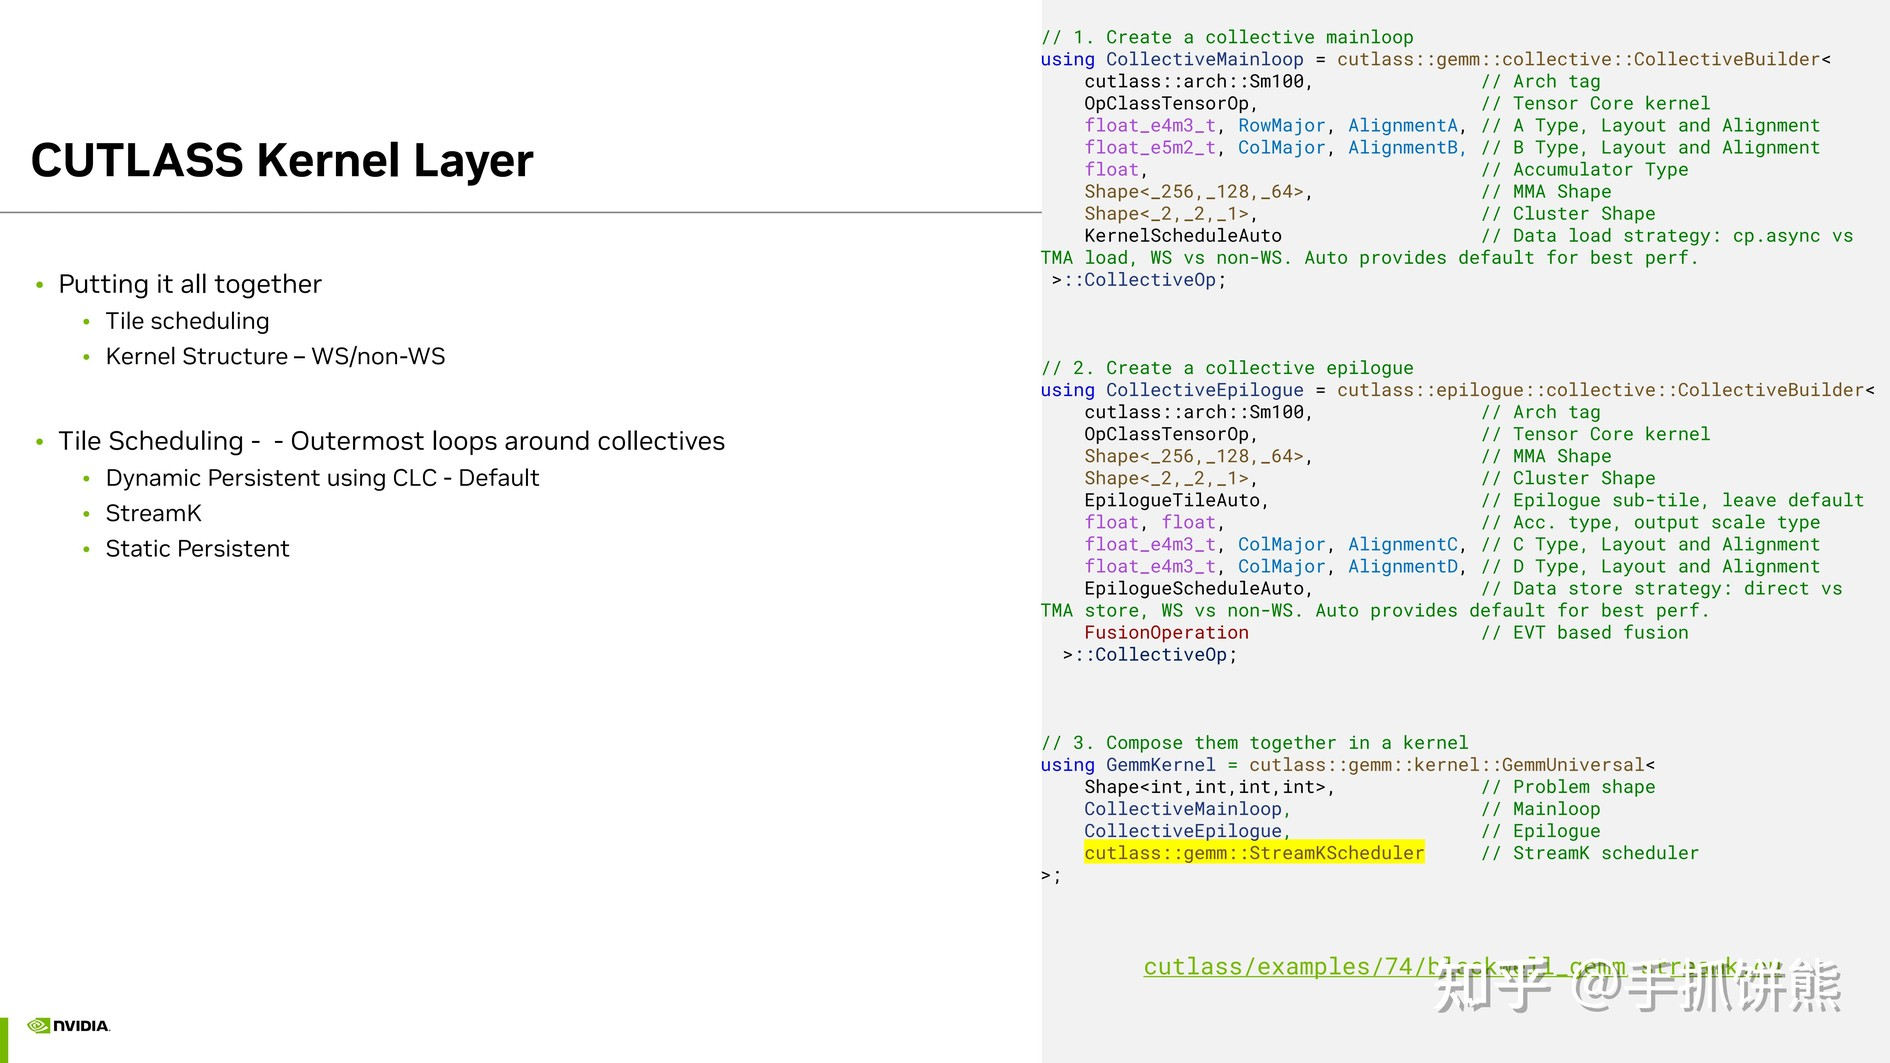
\includegraphics[width=0.9\textwidth]{figures/zhaoshangchun-01-tensor-core-programming/fig-68.jpg}
\end{figure}

这一页深入探讨了 \texttt{CUTLASS Kernel Layer} 的一个关键方面：\textbf{Tile 调度（Tile Scheduling）}。在 \texttt{Gemm\allowbreak{}Universal} 的组合示例中，第四个模板参数——\texttt{Scheduler}——被明确指定为 \texttt{c\allowbreak{}u\allowbreak{}t\allowbreak{}l\allowbreak{}a\allowbreak{}s\allowbreak{}s\allowbreak{}:\allowbreak{}:\allowbreak{}g\allowbreak{}e\allowbreak{}m\allowbreak{}m\allowbreak{}:\allowbreak{}:\allowbreak{}S\allowbreak{}t\allowbreak{}r\allowbreak{}e\allowbreak{}a\allowbreak{}m\allowbreak{}K\allowbreak{}S\allowbreak{}c\allowbreak{}h\allowbreak{}e\allowbreak{}d\allowbreak{}u\allowbreak{}l\allowbreak{}e\allowbreak{}r}。这标志着从默认的动态调度切换到了专门为处理 K 维度并行而设计的 \textbf{Stream-K 调度算法}。

传统的 GEMM 并行策略通常在 M 和 N 维度上划分 Tile，每个线程块（CTA）独立计算输出矩阵 C 的一个子块。这种方法在 M 和 N 很大时工作良好。但当 M 或 N 较小，而 K 维度很长时（即所谓的“瘦长”或“扁平”矩阵），仅在 M/\allowbreak{}N 维度上划分会导致并行度不足，大量 SM 闲置。

\textbf{Stream-K} 是一种专门解决这个问题的调度算法。它的核心思想是：\textbf{在 K 维度上进行切分，并将这些 K 维度的“块”分配给不同的 CTA Clusters 或 SMs}。计算完成后，不同 SM 上得到的中间累加结果需要进行一次并行的全局归约（Reduction），才能得到最终的 C 矩阵 Tile。

\begin{itemize}
\item \textbf{K 维度切分 (Splitting K)}：将 GEMM \texttt{C = A * B} 分解为多个子问题 \texttt{C\_\allowbreak{}i = A\_\allowbreak{}i * B\_\allowbreak{}i}，其中 \texttt{A\_\allowbreak{}i} 和 \texttt{B\_\allowbreak{}i} 是原始矩阵在 K 维度上的分片。
\item \textbf{并行计算}：多个 CTA 或 CTA 集群同时计算这些子问题。
\item \textbf{全局归约}：所有子问题计算完成后，需要一个额外的步骤将所有的 \texttt{C\_\allowbreak{}i} 相加（\texttt{C = sum(C\_\allowbreak{}i)}）。这个归约操作通常需要跨 SM 的同步和通信。
\end{itemize}

在 CUTLASS 中，\texttt{c\allowbreak{}u\allowbreak{}t\allowbreak{}l\allowbreak{}a\allowbreak{}s\allowbreak{}s\allowbreak{}:\allowbreak{}:\allowbreak{}g\allowbreak{}e\allowbreak{}m\allowbreak{}m\allowbreak{}:\allowbreak{}:\allowbreak{}S\allowbreak{}t\allowbreak{}r\allowbreak{}e\allowbreak{}a\allowbreak{}m\allowbreak{}K\allowbreak{}S\allowbreak{}c\allowbreak{}h\allowbreak{}e\allowbreak{}d\allowbreak{}u\allowbreak{}l\allowbreak{}e\allowbreak{}r} 封装了 Stream-K 算法的复杂调度和同步逻辑。

\begin{itemize}
\item \textbf{与 Mainloop/\allowbreak{}Epilogue 的协同}：Stream-K 调度器与 \texttt{Collective\allowbreak{}Mainloop} 和 \texttt{Collective\allowbreak{}Epilogue} 协同工作。Mainloop 负责处理 K 维度的单个分片，而 Epilogue 则可能需要处理局部的累加结果，或者在最终归约步骤中被调用。
\item \textbf{自动处理归约}：开发者只需在 \texttt{Gemm\allowbreak{}Universal} 中指定 \texttt{Stream\allowbreak{}KScheduler}，CUTLASS 就会自动生成归约所需的代码，包括跨 SM 的同步（可能利用 \texttt{mbarrier} 或其他原子操作）。这极大地降低了实现 Stream-K 的复杂度。
\item \textbf{性能提升}：对于 \texttt{GEMM} 中 \texttt{K} 维度远大于 \texttt{M} 和 \texttt{N} 维度的场景（例如某些 NLP 模型的特定层），使用 Stream-K 可以\textbf{显著提升 GPU 的利用率和整体吞吐}。它通过挖掘 K 维度的并行性，将原本受限于 M/\allowbreak{}N 维度的并行度扩展到了 K 维度，从而让更多的 SM 参与到计算中来。
\end{itemize}

此页还列出了 CUTLASS 支持的其他调度策略，形成了一个完整的调度器选项光谱：

\begin{itemize}
\item \textbf{\texttt{D\allowbreak{}y\allowbreak{}n\allowbreak{}a\allowbreak{}m\allowbreak{}i\allowbreak{}c\allowbreak{} \allowbreak{}P\allowbreak{}e\allowbreak{}r\allowbreak{}s\allowbreak{}i\allowbreak{}s\allowbreak{}t\allowbreak{}e\allowbreak{}n\allowbreak{}t\allowbreak{} \allowbreak{}u\allowbreak{}s\allowbreak{}i\allowbreak{}n\allowbreak{}g\allowbreak{} \allowbreak{}C\allowbreak{}L\allowbreak{}C\allowbreak{} \allowbreak{}-\allowbreak{} \allowbreak{}D\allowbreak{}e\allowbreak{}f\allowbreak{}a\allowbreak{}u\allowbreak{}l\allowbreak{}t}}：这是 Blackwell 上的默认选项，适用于大多数通用 GEMM 场景，提供良好的负载均衡。
\item \textbf{\texttt{Stream\allowbreak{}K}}：专门针对 K 维度并行设计的调度器，是解决“瘦长”矩阵性能问题的利器。
\item \textbf{\texttt{Static Persistent}}：一种静态调度策略，在编译时就确定好每个 CTA 的任务。它开销最小，但对负载均衡不友好，只适合那些形状非常规整、易于静态划分的 GEMM 问题。
\end{itemize}

对于 CUDA 工程师而言，这意味着在进行性能优化时，除了调整 Tile 形状和选择 Mainloop/\allowbreak{}Epilogue 策略外，\textbf{选择合适的调度器}也成为了一个重要的优化杠杆。通过 \texttt{7\allowbreak{}4\allowbreak{}/\allowbreak{}b\allowbreak{}l\allowbreak{}a\allowbreak{}c\allowbreak{}k\allowbreak{}w\allowbreak{}e\allowbreak{}l\allowbreak{}l\allowbreak{}\_\allowbreak{}g\allowbreak{}e\allowbreak{}m\allowbreak{}m\allowbreak{}\_\allowbreak{}s\allowbreak{}t\allowbreak{}r\allowbreak{}e\allowbreak{}a\allowbreak{}m\allowbreak{}k\allowbreak{}.\allowbreak{}c\allowbreak{}u} 这个示例，开发者可以学习如何在自己的代码中集成和测试 \texttt{Stream\allowbreak{}KScheduler}，以应对各种不同形状的矩阵乘法挑战。

\textbf{第 70 页：Kernel Layer 的结构：Warp-Specialized 内核}

\begin{figure}[H]\centering
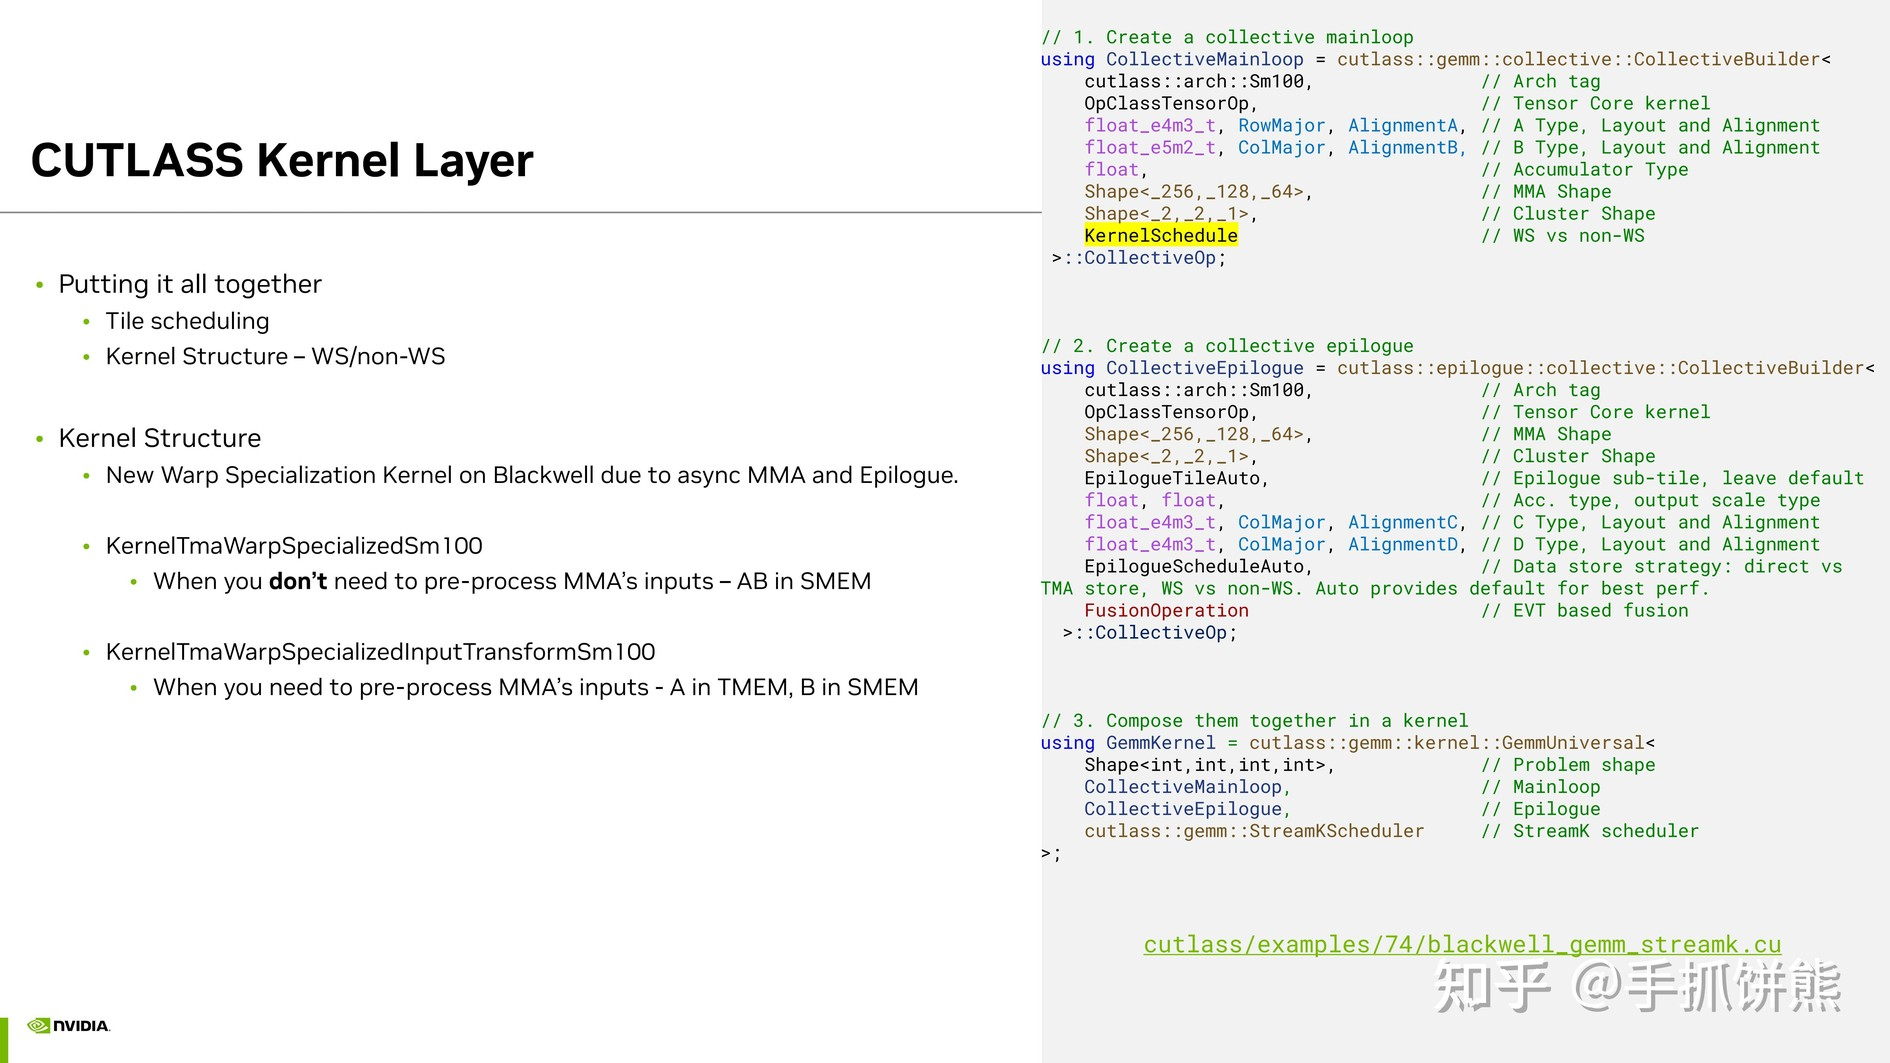
\includegraphics[width=0.9\textwidth]{figures/zhaoshangchun-01-tensor-core-programming/fig-69.jpg}
\end{figure}

继调度策略之后，这一页将焦点转向 \texttt{CUTLASS Kernel Layer} 的另一个核心职责：\textbf{内核结构（Kernel Structure）} 的选择。具体来说，它介绍了 Blackwell 架构上新的 Warp-Specialized (WS) 内核实现，这些实现是为了更好地适应异步 MMA 和 Epilogue 而设计的。

在 Blackwell 上，由于引入了 TMA（Tensor Memory Accelerator）以及更深层次的异步操作，传统的 WS 内核结构也随之演进。PPT 中提到了两种新的内核结构：

\begin{enumerate}
\item \textbf{\texttt{K\allowbreak{}e\allowbreak{}r\allowbreak{}n\allowbreak{}e\allowbreak{}l\allowbreak{}T\allowbreak{}m\allowbreak{}a\allowbreak{}W\allowbreak{}a\allowbreak{}r\allowbreak{}p\allowbreak{}S\allowbreak{}p\allowbreak{}e\allowbreak{}c\allowbreak{}i\allowbreak{}a\allowbreak{}l\allowbreak{}i\allowbreak{}z\allowbreak{}e\allowbreak{}d\allowbreak{}S\allowbreak{}m\allowbreak{}1\allowbreak{}0\allowbreak{}0}}：这是 Blackwell 上标准的 WS 内核结构。它假设 GEMM 的输入矩阵 A 和 B 都已经通过某种方式加载到了\textbf{共享内存（SMEM）}中。Mainloop 中的 MMA 指令直接从 SMEM 中读取数据进行计算。这种结构适用于\textbf{不需要对 MMA 的输入进行额外预处理}的场景。其流水线通常是：TMA 从 Global Memory (GMEM) 异步加载数据到 SMEM，然后 MMA Warps 从 SMEM 读取数据进行计算，同时 Epilogue Warps 处理前一轮的累加结果并写回。
\item \textbf{\texttt{K\allowbreak{}e\allowbreak{}r\allowbreak{}n\allowbreak{}e\allowbreak{}l\allowbreak{}T\allowbreak{}m\allowbreak{}a\allowbreak{}W\allowbreak{}a\allowbreak{}r\allowbreak{}p\allowbreak{}S\allowbreak{}p\allowbreak{}e\allowbreak{}c\allowbreak{}i\allowbreak{}a\allowbreak{}l\allowbreak{}i\allowbreak{}z\allowbreak{}e\allowbreak{}d\allowbreak{}I\allowbreak{}n\allowbreak{}p\allowbreak{}u\allowbreak{}t\allowbreak{}T\allowbreak{}r\allowbreak{}a\allowbreak{}n\allowbreak{}s\allowbreak{}f\allowbreak{}o\allowbreak{}r\allowbreak{}m\allowbreak{}S\allowbreak{}m\allowbreak{}1\allowbreak{}0\allowbreak{}0}}：这是一种更特殊的 WS 内核结构，它被设计用来处理\textbf{需要对 MMA 输入进行预处理}的场景。具体来说，它假设矩阵 A 的数据在\textbf{线程块内存（TMEM）}中，而矩阵 B 的数据在共享内存（SMEM）中。TMEM 是比 SMEM 更靠近计算核心的存储层次，通常用于存放需要频繁、低延迟访问的数据。这种结构可能用于需要对 A 矩阵进行实时（On-the-fly）转置、格式转换或其他复杂变换的场景，通过将 A 放在 TMEM 中可以加速这些预处理操作。
\end{enumerate}

Blackwell 架构的 WS 内核演进，其根本驱动力在于\textbf{最大化异步操作的重叠}。

\begin{itemize}
\item \textbf{异步 MMA (Async MMA)}：Blackwell 的 Tensor Core (TCGen05) 支持更深度的异步 MMA 操作。这意味着一旦发起了 MMA 指令，计算核心可以继续执行其他指令，而无需等待 MMA 完成。
\item \textbf{异步 Epilogue (Async Epilogue)}：如前所述，通过 TMA Store，Epilogue 的数据写回过程也是异步的。
\item \textbf{新的 WS 结构}：为了充分利用这两个层面的异步性，新的 WS 内核结构需要更精细地协调不同 Warp 组（数据加载 Warps、MMA Warps、Epilogue Warps）之间的工作。例如，通过 \texttt{mbarrier} 等同步原语，确保 MMA Warps 总能及时获取到加载完成的数据，同时 Epilogue Warps 也能在 MMA 计算出结果后立即开始工作。这种精细的流水线设计是 \texttt{K\allowbreak{}e\allowbreak{}r\allowbreak{}n\allowbreak{}e\allowbreak{}l\allowbreak{}T\allowbreak{}m\allowbreak{}a\allowbreak{}W\allowbreak{}a\allowbreak{}r\allowbreak{}p\allowbreak{}S\allowbreak{}p\allowbreak{}e\allowbreak{}c\allowbreak{}i\allowbreak{}a\allowbreak{}l\allowbreak{}i\allowbreak{}z\allowbreak{}e\allowbreak{}d\allowbreak{}S\allowbreak{}m\allowbreak{}1\allowbreak{}0\allowbreak{}0} 等新结构的核心。
\end{itemize}

对于开发者来说，这页内容提供了关于如何选择内核结构的具体指导。

\begin{itemize}
\item \textbf{默认选择 \texttt{Kernel\allowbreak{}Schedule\allowbreak{}Auto}}：在 \texttt{Collective\allowbreak{}Mainloop} 的构建过程中，\texttt{Kernel\allowbreak{}Schedule} 参数如果设为 \texttt{Kernel\allowbreak{}Schedule\allowbreak{}Auto}，CUTLASS 会根据上下文自动选择合适的内核结构（WS vs. non-WS）和数据加载策略（TMA vs. \texttt{cp.\allowbreak{}async})。在大多数情况下，这是最省心且高效的选择。
\item \textbf{手动选择以进行精细优化}：当自动选择的性能不理想，或者开发者有明确的硬件资源使用规划时，可以手动指定 \texttt{Kernel\allowbreak{}Schedule}。例如，如果你确定你的算法不需要对输入进行任何变换，且希望最大化利用 SMEM 进行数据缓冲，那么可以倾向于选择 \texttt{K\allowbreak{}e\allowbreak{}r\allowbreak{}n\allowbreak{}e\allowbreak{}l\allowbreak{}T\allowbreak{}m\allowbreak{}a\allowbreak{}W\allowbreak{}a\allowbreak{}r\allowbreak{}p\allowbreak{}S\allowbreak{}p\allowbreak{}e\allowbreak{}c\allowbreak{}i\allowbreak{}a\allowbreak{}l\allowbreak{}i\allowbreak{}z\allowbreak{}e\allowbreak{}d\allowbreak{}S\allowbreak{}m\allowbreak{}1\allowbreak{}0\allowbreak{}0} 相关的策略。
\item \textbf{处理复杂输入的场景}：如果你的算法需要在 GEMM 主循环中对输入数据（如 A 矩阵）进行复杂的、需要低延迟访存的预处理，那么 \texttt{K\allowbreak{}e\allowbreak{}r\allowbreak{}n\allowbreak{}e\allowbreak{}l\allowbreak{}T\allowbreak{}m\allowbreak{}a\allowbreak{}W\allowbreak{}a\allowbreak{}r\allowbreak{}p\allowbreak{}S\allowbreak{}p\allowbreak{}e\allowbreak{}c\allowbreak{}i\allowbreak{}a\allowbreak{}l\allowbreak{}i\allowbreak{}z\allowbreak{}e\allowbreak{}d\allowbreak{}I\allowbreak{}n\allowbreak{}p\allowbreak{}u\allowbreak{}t\allowbreak{}T\allowbreak{}r\allowbreak{}a\allowbreak{}n\allowbreak{}s\allowbreak{}f\allowbreak{}o\allowbreak{}r\allowbreak{}m\allowbreak{}S\allowbreak{}m\allowbreak{}1\allowbreak{}0\allowbreak{}0} 就提供了一个可能的优化方向。这在一些非标准的 GEMM 或计算密集型预处理场景中可能非常有用。
\end{itemize}

总而言之，CUTLASS 4.0 不仅提供了高层抽象，也保留了底层控制的灵活性。通过 \texttt{Kernel\allowbreak{}Schedule} 参数，高级用户可以深入到内核结构的层面，根据自己对算法和硬件的理解，进行更精细的性能调优。这体现了 CUTLASS 作为“专家级”工具库的设计哲学：既要易于上手，也要有足够的深度供专家挖掘。

\textbf{第 71 页：Warp-Specialized 持久化内核：Hopper vs. Blackwell}

\begin{figure}[H]\centering
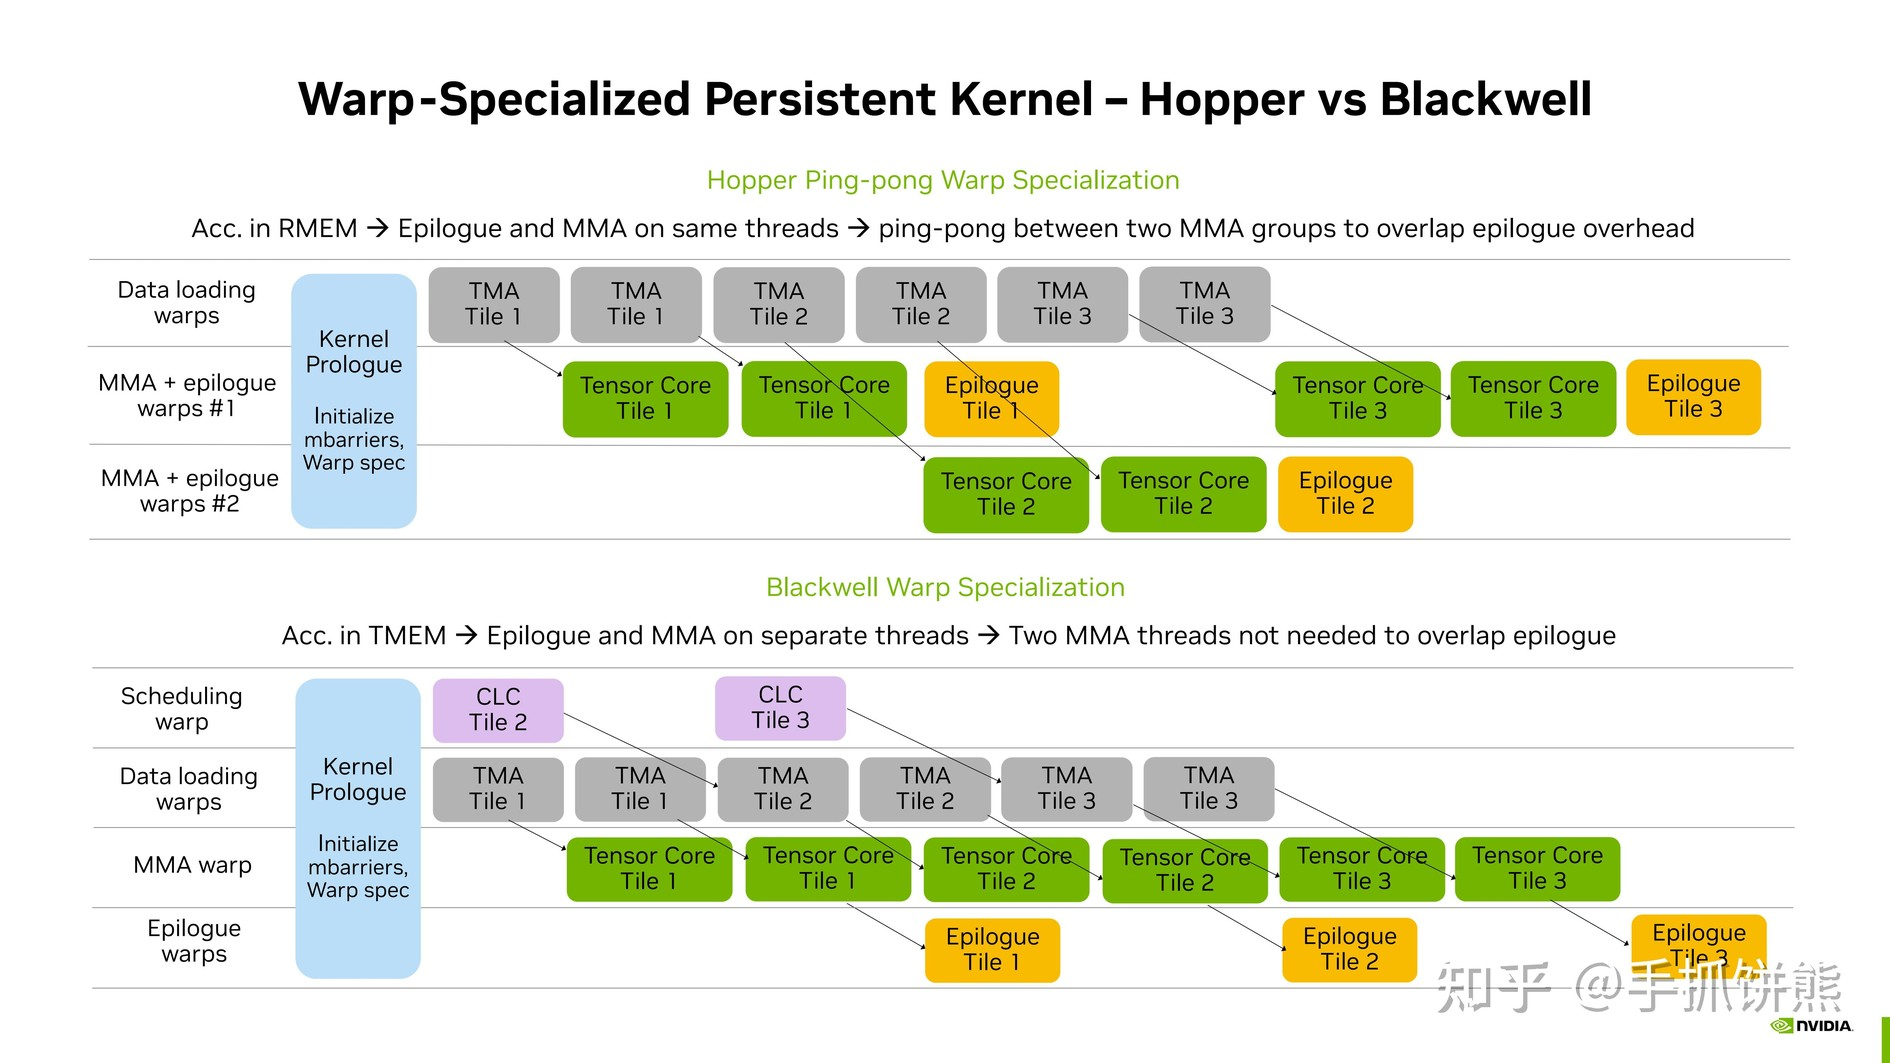
\includegraphics[width=0.9\textwidth]{figures/zhaoshangchun-01-tensor-core-programming/fig-70.jpg}
\end{figure}

这一页通过两张对比图，直观地展示了 Warp-Specialized (WS) 持久化内核在 Hopper 和 Blackwell 架构上的关键差异。这种对比深刻地揭示了 Blackwell 硬件特性的演进如何直接影响了软件层面的流水线设计和性能优化策略。

左图展示了 Hopper 架构上的 WS 内核流水线。其核心特点是：

\begin{itemize}
\item \textbf{累加结果在寄存器（RMEM）}：MMA 的累加结果（Accumulators）直接存放在 Warps 的寄存器文件中。
\item \textbf{MMA 和 Epilogue 由同一组线程执行}：执行 MMA 计算的 Warp（或 Warp 组）在计算完成后，需要“亲自”执行 Epilogue 操作。这意味着计算和后处理是串行的。
\item \textbf{Ping-pong 结构以重叠开销}：为了掩盖 Epilogue 的执行开销，Hopper 的 WS 内核采用了一种巧妙的“乒乓（Ping-pong）”策略。一个 CTA 内的 MMA Warps 被分为两组（\texttt{MMA + epilogue warps \#1} 和 \texttt{MMA + epilogue warps \#2}）。当第一组在执行 Tile 1 的 Epilogue 时，第二组可以开始计算 Tile 2 的 MMA。反之亦然。通过这种方式，Epilogue 的延迟被另一组的 MMA 计算所隐藏。
\item \textbf{调度}：\texttt{Data loading warps} 负责从 GMEM 加载数据，并通过 \texttt{mbarrier} 与 MMA/\allowbreak{}Epilogue Warps 同步。
\end{itemize}

这种设计的\textbf{优点}是结构相对清晰，且有效地重叠了计算和后处理。但\textbf{缺点}是它强迫 MMA 和 Epilogue 绑定在同一组线程上，并且需要两组 MMA Warps 来实现流水线，对寄存器和线程资源有一定压力。

右图展示了 Blackwell 架构上更为先进的 WS 内核流水线，其变化是革命性的：

\begin{itemize}
\item \textbf{累加结果在线程块内存（TMEM）}：这是最核心的变化。MMA 的累加结果被直接输出到 SM 内一块专用的、高速的线程块内存（TMEM）中。TMEM 对于整个线程块内的所有 Warps 都是可见的。
\item \textbf{MMA 和 Epilogue 角色彻底解耦}：由于累加结果位于共享的 TMEM 中，执行 Epilogue 的 Warp 不再需要是执行 MMA 的那一组 Warp。这使得 \textbf{MMA Warps} 和 \textbf{Epilogue Warps} 可以成为两个完全独立的、并行的角色。MMA Warps 只负责不停地计算，并将结果“扔”到 TMEM 中；而 Epilogue Warps 则独立地从 TMEM 中取出结果，进行后处理和写回。
\item \textbf{不再需要 Ping-pong}：因为 MMA 和 Epilogue 的执行者被解耦，它们可以自然地形成一个生产者-消费者流水线。MMA Warps 作为生产者，Epilogue Warps 作为消费者。不再需要两组 MMA Warps 来进行乒乓操作，\textbf{一组 MMA Warp 就足以和 Epilogue Warp 形成高效流水线}。
\item \textbf{调度}：流水线变得更长、更专业化。除了 \texttt{Data loading warps} 和 \texttt{MMA warp}，还出现了专门的 \texttt{Epilogue warps} 和一个可选的 \texttt{Scheduling warp}（可能用于 CLC 动态调度）。
\end{itemize}

从 Hopper 到 Blackwell 的演进，对 CUDA 性能优化工程师意味着：

\begin{itemize}
\item \textbf{更高的硬件利用率}：Blackwell 的设计释放了更多的线程资源。原本需要两组 MMA Warps 才能实现的流水线，现在一组就够了。这使得每个 CTA 可以容纳更多的活动 Warp，或者可以将省下来的资源用于更深的流水线缓冲（Pipelining Depth），从而更好地隐藏延迟，提升 SM 的利用率。
\item \textbf{更灵活的流水线设计}：角色的彻底解耦给予了开发者更大的灵活性。例如，可以根据计算和 Epilogue 的相对开销，动态地调整分配给 MMA Warps 和 Epilogue Warps 的线程数量，以达到最佳的平衡。
\item \textbf{简化的内核逻辑}：尽管流水线本身更复杂，但每个角色的逻辑却可能更简单。MMA Warp 只需关注计算，Epilogue Warp 只需关注后处理。这种“职责分离”使得代码更易于理解和维护，也降低了编写复杂融合内核的心智负担。
\item \textbf{对 CUTLASS 的依赖增强}：这种高度复杂的、依赖硬件特性的流水线调度，手动编写和调优的难度极大。这进一步凸显了 CUTLASS 这类高级库的价值。开发者通过 \texttt{Collective\allowbreak{}Builder} 和 \texttt{Gemm\allowbreak{}Universal}，实际上是在利用 NVIDIA 工程师对 Blackwell 架构的最佳理解，自动生成了如图所示的高效流水线代码。
\end{itemize}

总而言之，第 71 页的对比清晰地表明，Blackwell 不仅仅是增加了计算单元，更是从体系结构层面重新设计了 SM 内的数据流和协作方式，为实现更高效率的软件流水线铺平了道路。

\section{五、\textbf{总结与未来展望}}

经过前面几章的深度探索，我们已经了解了 Blackwell 架构的硬件革新，以及 Cu\allowbreak{}Te 和 CUTLASS 4.0 是如何让我们能够驾驭这些新能力的。本章将对 CUTLASS 4.0 带来的新功能做一个全面的总结，并展望其未来的发展方向，为我们的技术探索画上一个圆满的句号。

\textbf{第 72 页：章节议程过渡}

\begin{figure}[H]\centering
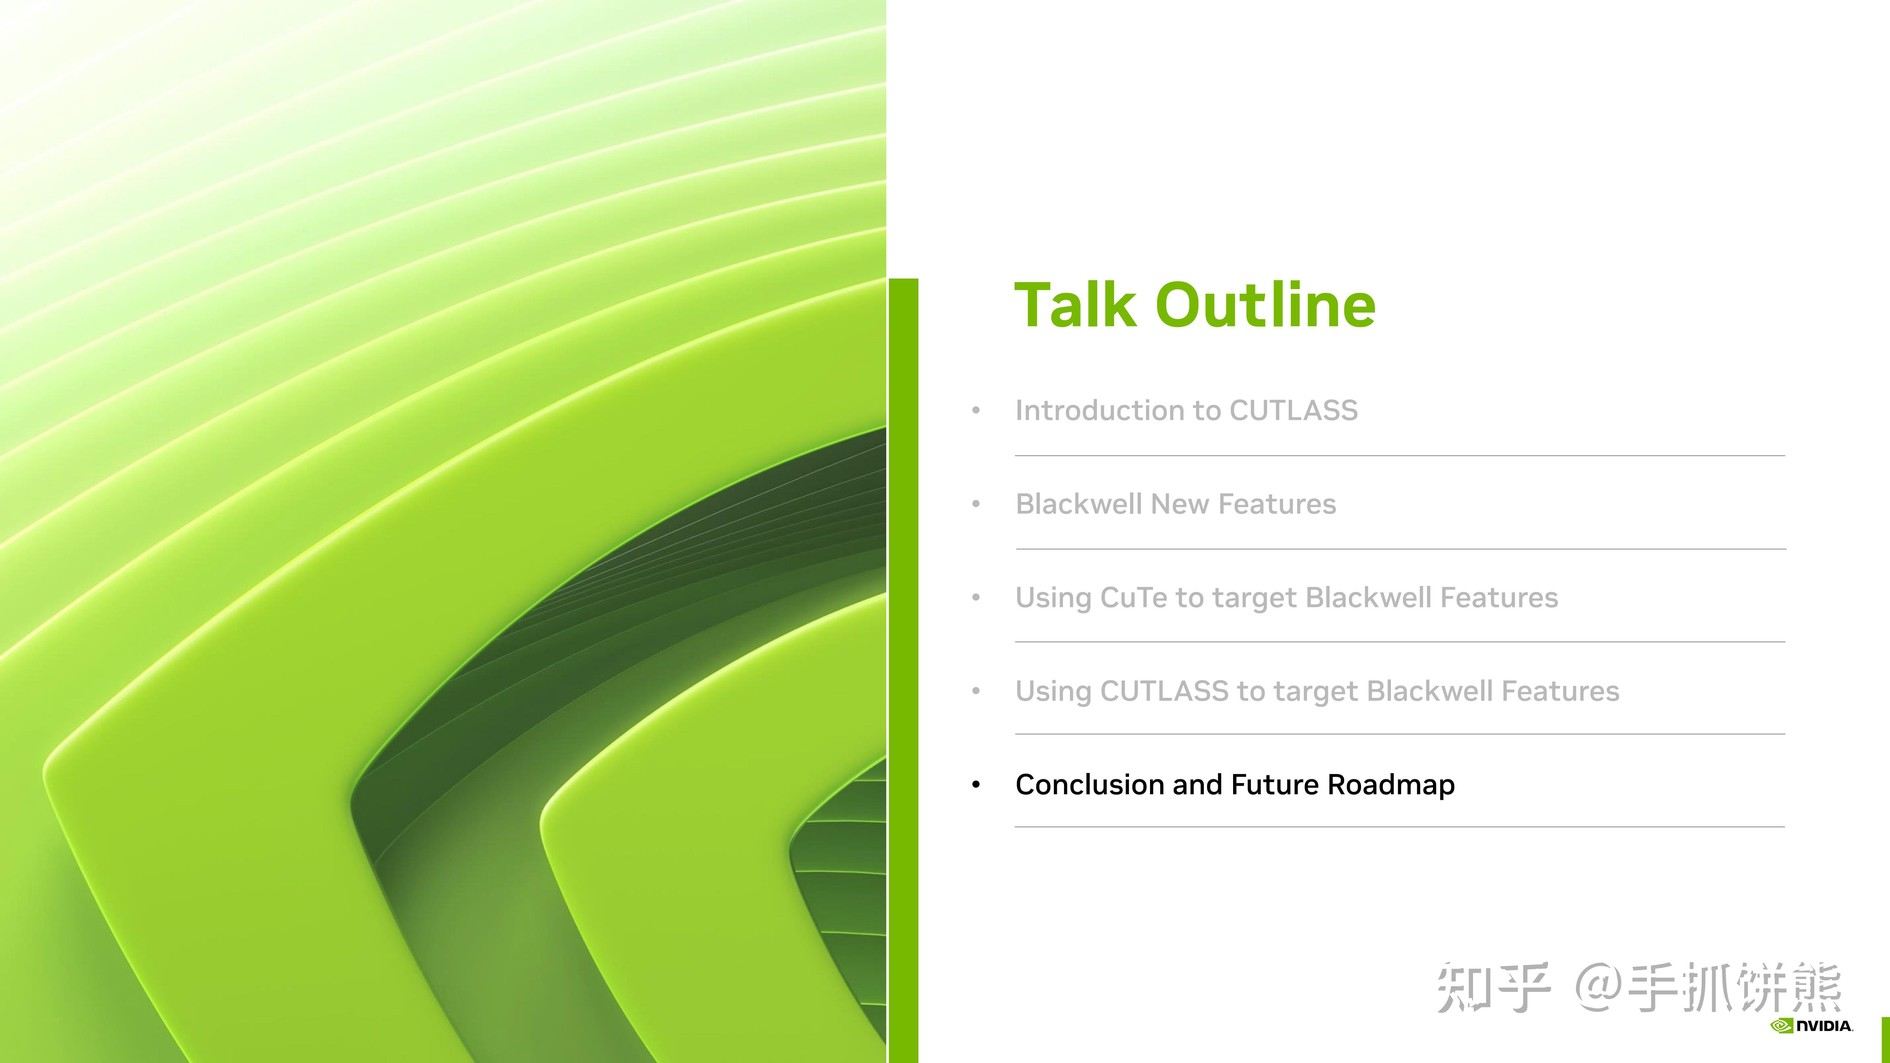
\includegraphics[width=0.9\textwidth]{figures/zhaoshangchun-01-tensor-core-programming/fig-71.jpg}
\end{figure}

这张大纲页高亮了最后一个主题“Conclusion and Future Roadmap”，标志着我们的技术探索之旅即将到达终点。在深入了解了 Blackwell 的硬件细节和 CUTLASS 的编程模型之后，现在是时候退后一步，从一个更高的视角来审视 CUTLASS 的现状和未来。

对于工程团队来说，技术选型的决策不仅要看当前的功能是否满足需求，更要看其未来的发展潜力和社区的活跃度。这一章的内容，将为我们评估是否持续投资于 CUTLASS 生态提供重要的决策依据。

\textbf{第 73 页：CUTLASS 3.8 的新特性总结}

\begin{figure}[H]\centering
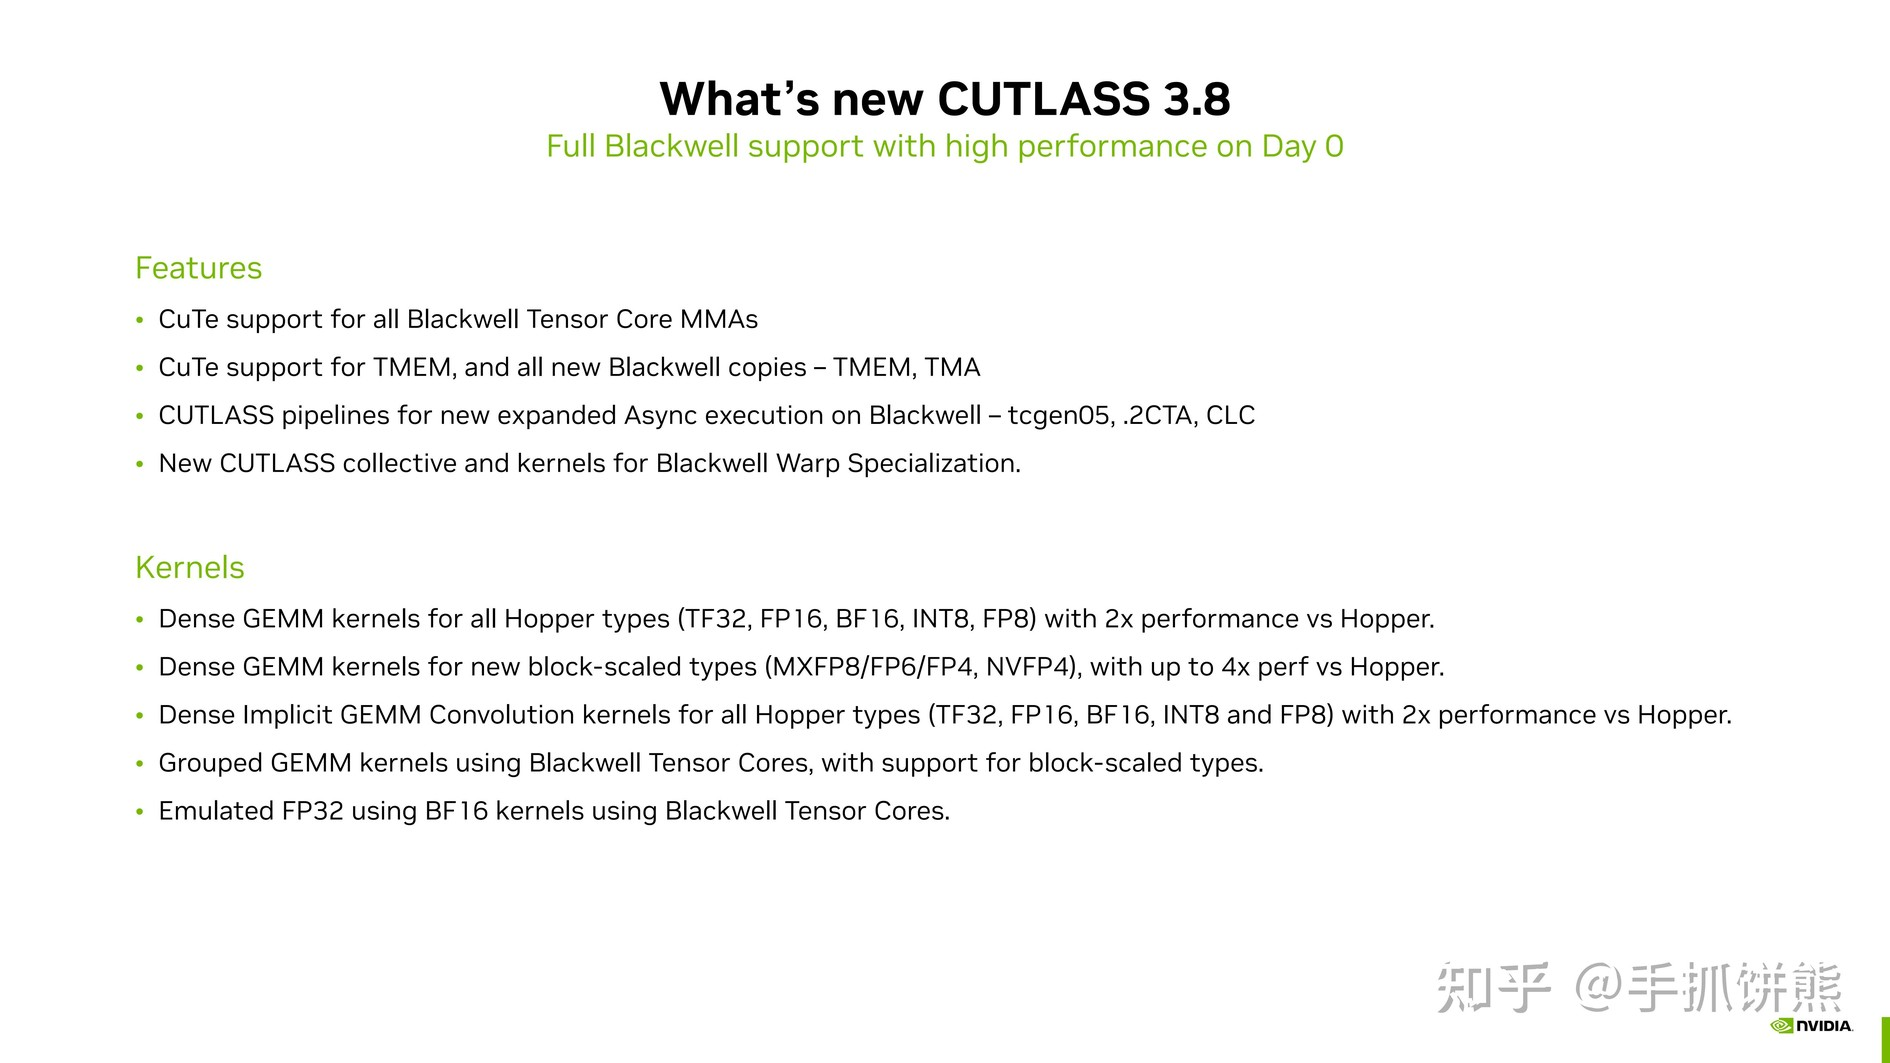
\includegraphics[width=0.9\textwidth]{figures/zhaoshangchun-01-tensor-core-programming/fig-72.jpg}
\end{figure}

这一页是对 CUTLASS 3.8 版本（即支持 Blackwell 的首个版本，可视为 CUTLASS 4.0 的前身）新功能的全面总结，它展示了 CUTLASS 对 Blackwell 架构的 \textbf{Day 0 高性能支持}。这包括对 \texttt{tcgen05} MMA 指令、TMEM 操作的全面适配，为 Blackwell 异步模型设计的全新软件流水线，以及一系列开箱即用的、性能翻倍的 GEMM、卷积、Grouped GEMM 等核函数。

特别值得注意的是，CUTLASS 为 Blackwell 新增的 MXFP8/\allowbreak{}FP6/\allowbreak{}FP4 等块缩放数据类型也提供了完整的支持，最高可达 Hopper FP8 性能的 4 倍。这对需要极致推理性能和模型压缩率的场景来说是巨大的福音。这一系列坚实的功能更新，确保了开发者从第一天起就能通过 CUTLASS 充分挖掘 Blackwell 的巨大潜力，体现了 NVIDIA 在软硬件协同设计上的深厚功力。

\textbf{第 74 页：2025 年及未来的路线图}

\begin{figure}[H]\centering
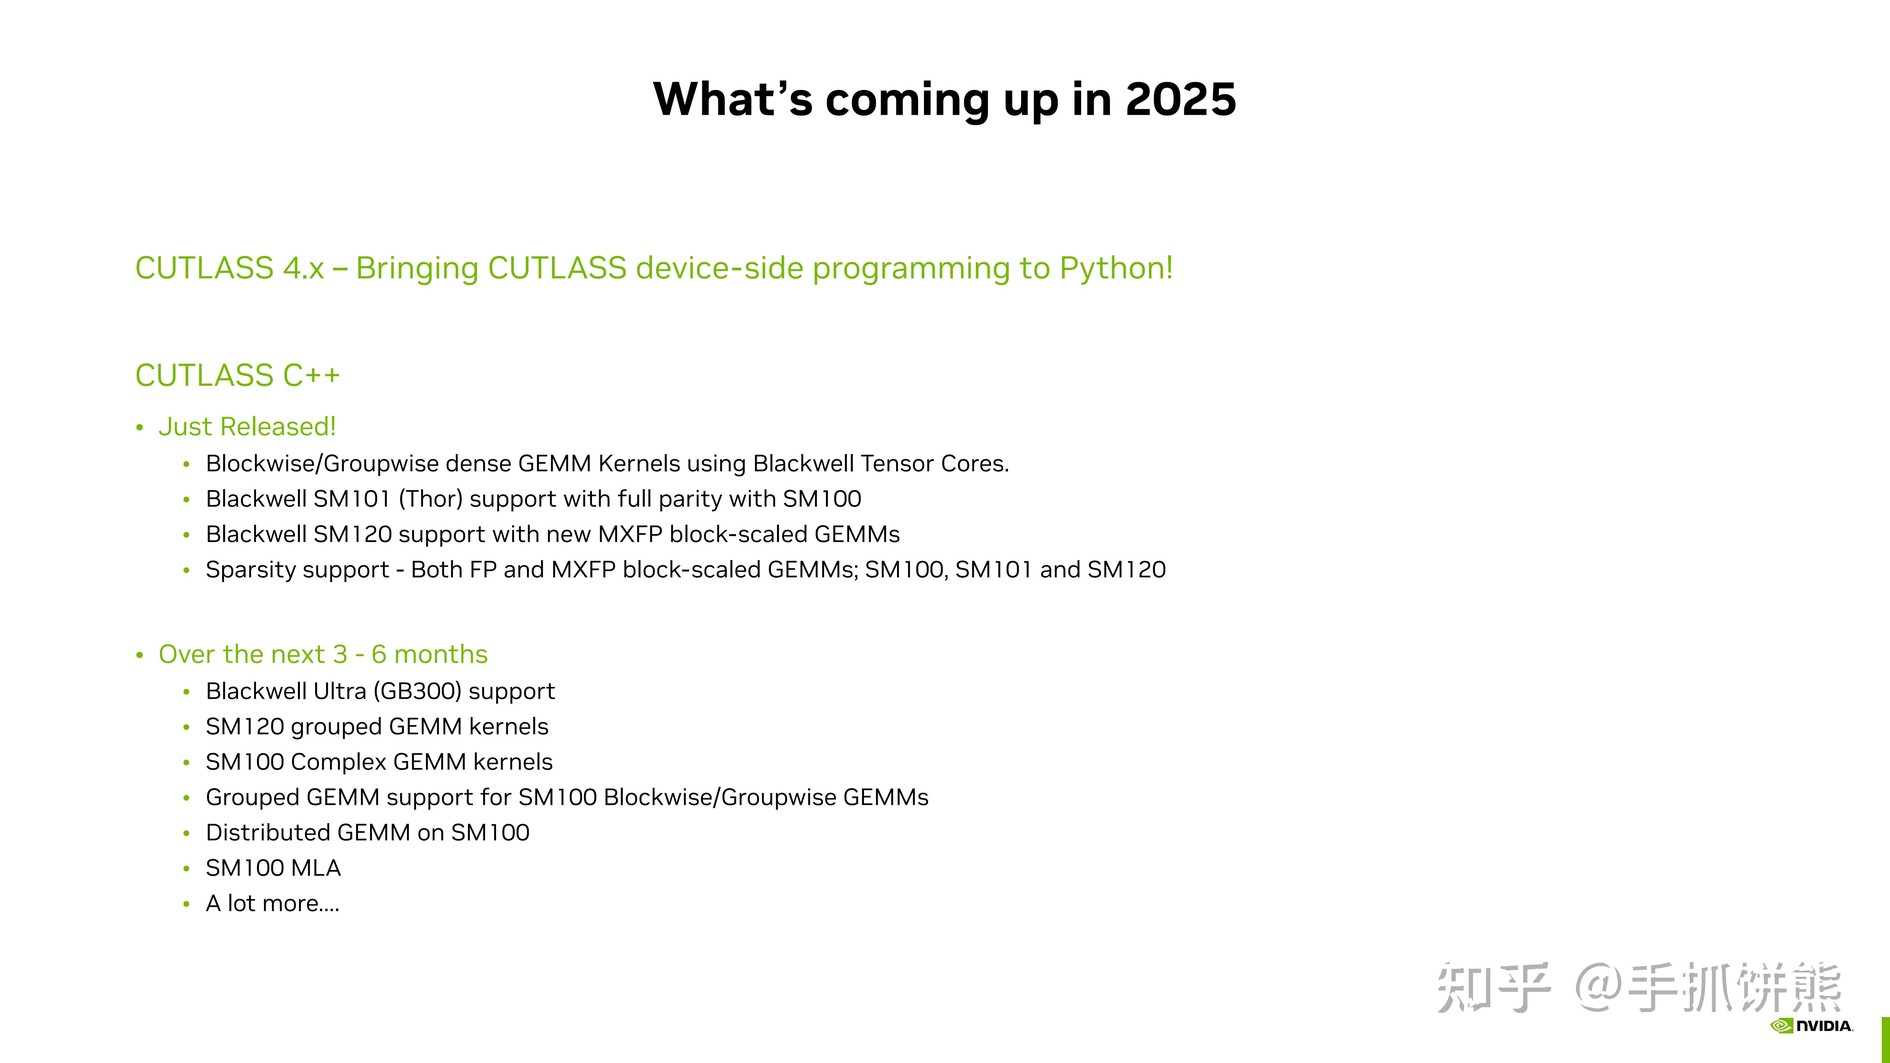
\includegraphics[width=0.9\textwidth]{figures/zhaoshangchun-01-tensor-core-programming/fig-73.jpg}
\end{figure}

这张幻灯片揭示了 CUTLASS 在 2025 年及以后的宏伟蓝图。最引人注目的莫过于 \textbf{CUTLASS 4.x 将引入 Python 编程接口}！这意味着开发者未来或许可以直接在 Python 中，以一种更简洁、更动态的方式来定义和生成高性能的 CUTLASS 核函数，这将极大地降低使用门槛，并加速研发迭代速度，让更多的算法工程师和研究者能够参与到算子优化的工作中来。

在具体功能方面，CUTLASS 的演进步伐并未停歇，计划支持 Blackwell Ultra (GB300)、分布式 GEMM (Distributed GEMM) 和混合精度 MLA (Mixed-Precision Low-Precision Accumulation) 等前沿领域。这表明 CUTLASS 社区展现了其旺盛的生命力和清晰的演进路径。它不仅紧跟 NVIDIA 硬件迭代的步伐，还在积极地向更易用、更强大的方向发展，持续投资于 CUTLASS 生态，无疑是保持技术领先的明智之举。

\textbf{第 75 页：致谢部分}

\begin{figure}[H]\centering
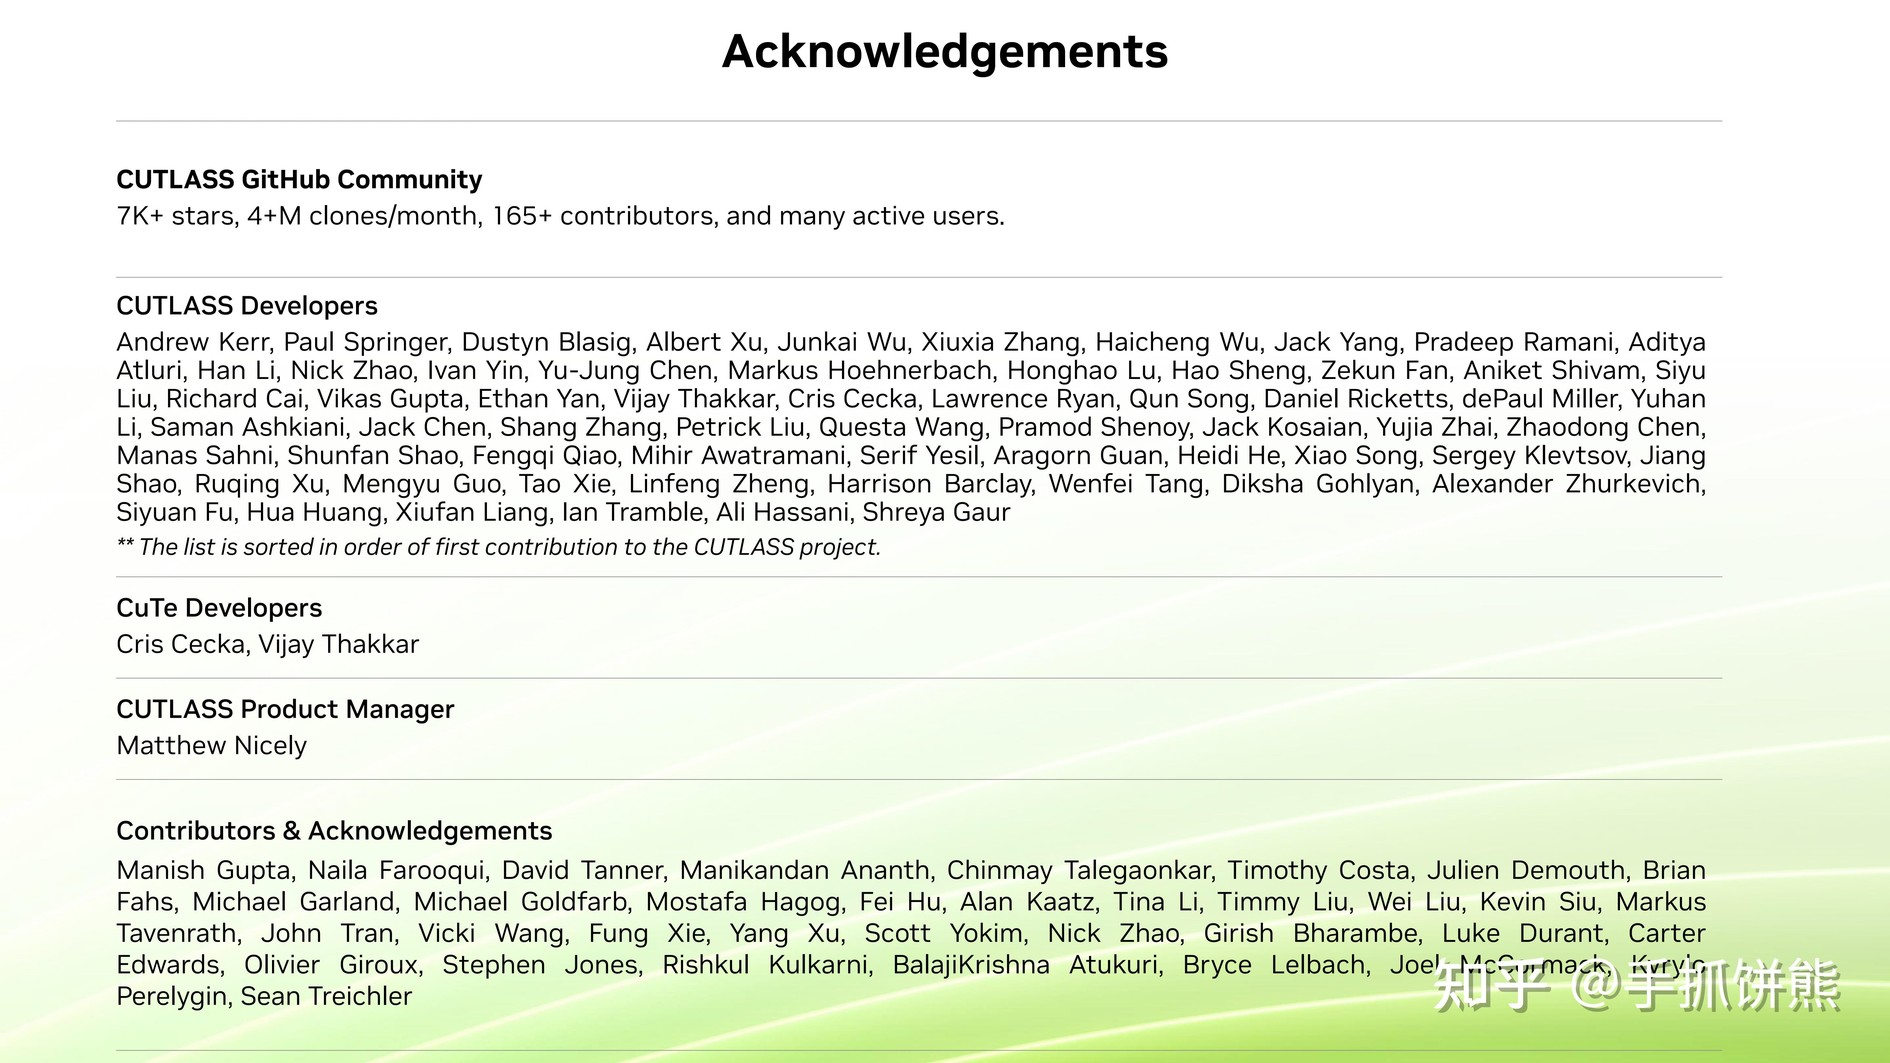
\includegraphics[width=0.9\textwidth]{figures/zhaoshangchun-01-tensor-core-programming/fig-74.jpg}
\end{figure}

最后的致谢页列出了为 CUTLASS 项目做出贡献的众多开发者、研究者和产品经理。

\endgroup
